%Este trabalho está licenciado sob a Licença Atribuição-CompartilhaIgual 4.0 Internacional Creative Commons. Para visualizar uma cópia desta licença, visite http://creativecommons.org/licenses/by-sa/4.0/deed.pt_BR ou mande uma carta para Creative Commons, PO Box 1866, Mountain View, CA 94042, USA.

\documentclass[12pt]{book}

\input ../preambulo.tex

\ifispython
\lstset { %
  language=Python,
}
\fi


\makeindex

\begin{document}

\frontmatter

\title{Matemática Numérica II}
\author{Pedro H A Konzen}
\date{\today}
\ifishtml
\else
\addcontentsline{toc}{chapter}{Capa}
\fi

\maketitle

%Este trabalho está licenciado sob a Licença Atribuição-CompartilhaIgual 4.0 Internacional Creative Commons. Para visualizar uma cópia desta licença, visite http://creativecommons.org/licenses/by-sa/4.0/ ou mande uma carta para Creative Commons, PO Box 1866, Mountain View, CA 94042, USA.

\chapter*{Licença}\label{licenca}
\addcontentsline{toc}{chapter}{Licença}

Este trabalho está licenciado sob a Licença Atribuição-CompartilhaIgual 4.0 Internacional Creative Commons. Para visualizar uma cópia desta licença, visite http://creativecommons.org/licenses/by-sa/4.0/deed.pt\_BR ou mande uma carta para Creative Commons, PO Box 1866, Mountain View, CA 94042, USA.

%Este trabalho está licenciado sob a Licença Atribuição-CompartilhaIgual 4.0 Internacional Creative Commons. Para visualizar uma cópia desta licença, visite http://creativecommons.org/licenses/by-sa/4.0/deed.pt_BR ou mande uma carta para Creative Commons, PO Box 1866, Mountain View, CA 94042, USA.

\chapter*{Prefácio}\label{prefacio}
\addcontentsline{toc}{chapter}{Prefácio}

O site \href{https://www.notaspedrok.com.br}{notaspedrok.com.br} é uma plataforma que construí para o compartilhamento de minhas notas de aula. Essas anotações feitas como preparação de aulas é uma prática comum de professoras/es. Muitas vezes feitas a rabiscos em rascunhos com validade tão curta quanto o momento em que são concebidas, outras vezes, com capricho de um diário guardado a sete chaves. Notas de aula também são feitas por estudantes - são anotações, fotos, prints, entre outras formas de registros de partes dessas mesmas aulas. Essa dispersão de material didático sempre me intrigou e foi o que me motivou a iniciar o site.

Com início em 2018, o site contava com apenas três notas incipientes. De lá para cá, conforme fui expandido e revisando os materais, o site foi ganhando acessos de vários locais do mundo, em especial, de países de língua portugusa. No momento, conta com 13 notas de aula, além de minicursos e uma coleção de vídeos e áudios.

As notas de \emph{Redes Neurais Artificiais} fazem uma introdução às redes neuraus artificiais com enfase na resolução de problemas de matemática. Como ferramenta de apoio computacional, códigos exemplos são trabalhos em linguagem {\python}, mais especificamente, com o pacote de aprendizagem de máquina {\pytorch}.

Aproveito para agradecer a todas/os que de forma assídua ou esporádica contribuem com correções, sugestões e críticas! ;)

\begin{flushright}
  Pedro H A Konzen

  \url{https://www.notaspedrok.com.br}
\end{flushright}



\tableofcontents
\addcontentsline{toc}{chapter}{Sumário}

\mainmatter

%%Este trabalho está licenciado sob a Licença Atribuição-CompartilhaIgual 4.0 Internacional Creative Commons. Para visualizar uma cópia desta licença, visite http://creativecommons.org/licenses/by-sa/4.0/deed.pt_BR ou mande uma carta para Creative Commons, PO Box 1866, Mountain View, CA 94042, USA.

\chapter{Introdução}\label{cap_intro}
\thispagestyle{fancy}

\begin{flushright}
  [Vídeo] | [Áudio] | \href{https://phkonzen.github.io/notas/contato.html}{[Contatar]}
\end{flushright}

\emconstrucao

%%Este trabalho está licenciado sob a Licença Atribuição-CompartilhaIgual 4.0 Internacional Creative Commons. Para visualizar uma cópia desta licença, visite http://creativecommons.org/licenses/by-sa/4.0/deed.pt_BR ou mande uma carta para Creative Commons, PO Box 1866, Mountain View, CA 94042, USA.

\chapter{Interpolação}\label{cap_interp}
\thispagestyle{fancy}

Neste capítulo, estudamos a \hl{resolução de problemas de interpolação} da forma: dados uma família de $n$ funções reais
\begin{equation}\hleq
  \mathcal{F} = \{f_1(x), f_2(x), \dotsc, f_n(x)\}
\end{equation}
e um conjunto de $n$ pontos $\{(x_i, y_i)\}_{i=1}^n$, com $x_i\neq x_j$ se $i\neq j$, encontrar a \emph{função interpoladora}
\begin{equation}\hleq
  f(x) = c_1f_1(x) + c_2f_2(x) + \cdots + c_nf_n(x),
\end{equation}
tal que
\begin{equation}\hleq
  y_i = f(x_i),\quad i=1, 2, \ldots, n.
\end{equation}

\section{Interpolação polinomial}\label{cap_interp_sec_interpoli}

\hl{Dado um conjunto de $n$ pontos $\{(x_i, y_i)\}_{i=1}^n$, o problema de interpolação consiste em encontrar o polinômio\footnote{Chamado de \emph{polinômio interpolador}.} de grau $n-1$}
\begin{equation}\label{cap_interp_sec_interpoli:eq:interpoli_poli}\hleq
  p(x) = p_1x^{n-1} + p_2x^{n-2} + \cdots + p_{n-1}x + p_n
\end{equation}
tal que
\begin{equation}\label{cap_interp_sec_interpoli:eq:interpoli_conds}\hleq
  y_i = p(x_i),
\end{equation}
para todo $i=1, 2, \dotsc, n$.

Das condições \eqref{cap_interp_sec_interpoli:eq:interpoli_poli}, temos
\begin{equation}
  \begin{aligned}\label{cap_interp_sec_interpoli:eq:interpoli_sis}
    p_1x_1^{n-1} + p_2x_1^{n-2} + \cdots + p_{n-1}x_1 + p_n &= y_1 \\
    p_1x_2^{n-1} + p_2x_2^{n-2} + \cdots + p_{n-1}x_2 + p_n &= y_2 \\
    &\vdots \\
    p_1x_n^{n-1} + p_2x_n^{n-2} + \cdots + p_{n-1}x_n + p_n &= y_n.
  \end{aligned}
\end{equation}
Isto é, \hl{os coeficientes do \emph{polinômio interpolador} {\eqref{cap_interp_sec_interpoli:eq:interpoli_poli}} satisfazem o sistema linear}
\begin{equation}\hleq
  A\pmb{p} = \pmb{y},
\end{equation}
onde $A$ é a \emph{matriz de Vandermonde}{\vandermonde}
\begin{equation}\hleq
  A =
  \begin{bmatrix}
    x_1^{n-1} & x_1^{n-2} & \ldots & x_1 & 1 \\
    x_2^{n-1} & x_2^{n-2} & \ldots & x_2 & 1 \\
    \vdots  & \vdots  & \vdots  & \vdots & \vdots \\
    x_n^{n-1} & x_n^{n-2} & \ldots & x_n & 1
  \end{bmatrix},
\end{equation}
$\pmb{p} = (p_1, p_2, \ldots, p_n)$ é o \emph{vetor das incógnitas} e $\pmb{y} = (y_1, y_2, \ldots, y_n)$ é o \emph{vetor dos termos constantes}.

\begin{ex}\label{cap_interp_sec_interpoli:ex:interpoli_intro}
  Consideramos o problema de encontrar o polinômio interpolador do conjunto de pontos $\{(-1,~-1), (0,~1), (1,~1/2)\}$. Como temos 3 pontos, o polinômio tem grau 2 e pode ser escrito na forma
  \begin{equation}
    p(x) = p_1x^2 + p_2x + p_3.
  \end{equation}
  Seguindo a abordagem acima, temos $\pmb{p}=(p_1, p_2, p_3)$, $\pmb{x} = (-1, 0, 1)$, $\pmb{y}=(-1, 1, 1/2)$ e
  \begin{equation}
    A =
    \begin{bmatrix}
      x_1^2 & x_1 & 1\\
      x_2^2 & x_2 & 1\\
      x_3^2 & x_3 & 1
    \end{bmatrix}.
  \end{equation}
  Então, resolvendo $A\pmb{p} = \pmb{y}$, obtemos o polinômio interpolador
  \begin{equation}
    p(x) = -1,25x^2 + 0,75x + 1.
  \end{equation}
A Figura \ref{cap_interp_sec_interpoli:fig:interpoli_intro} mostra os esboços do polinômio interpolador $p(x)$ e  dos pontos dados.

\begin{figure}[h!]
  \centering
  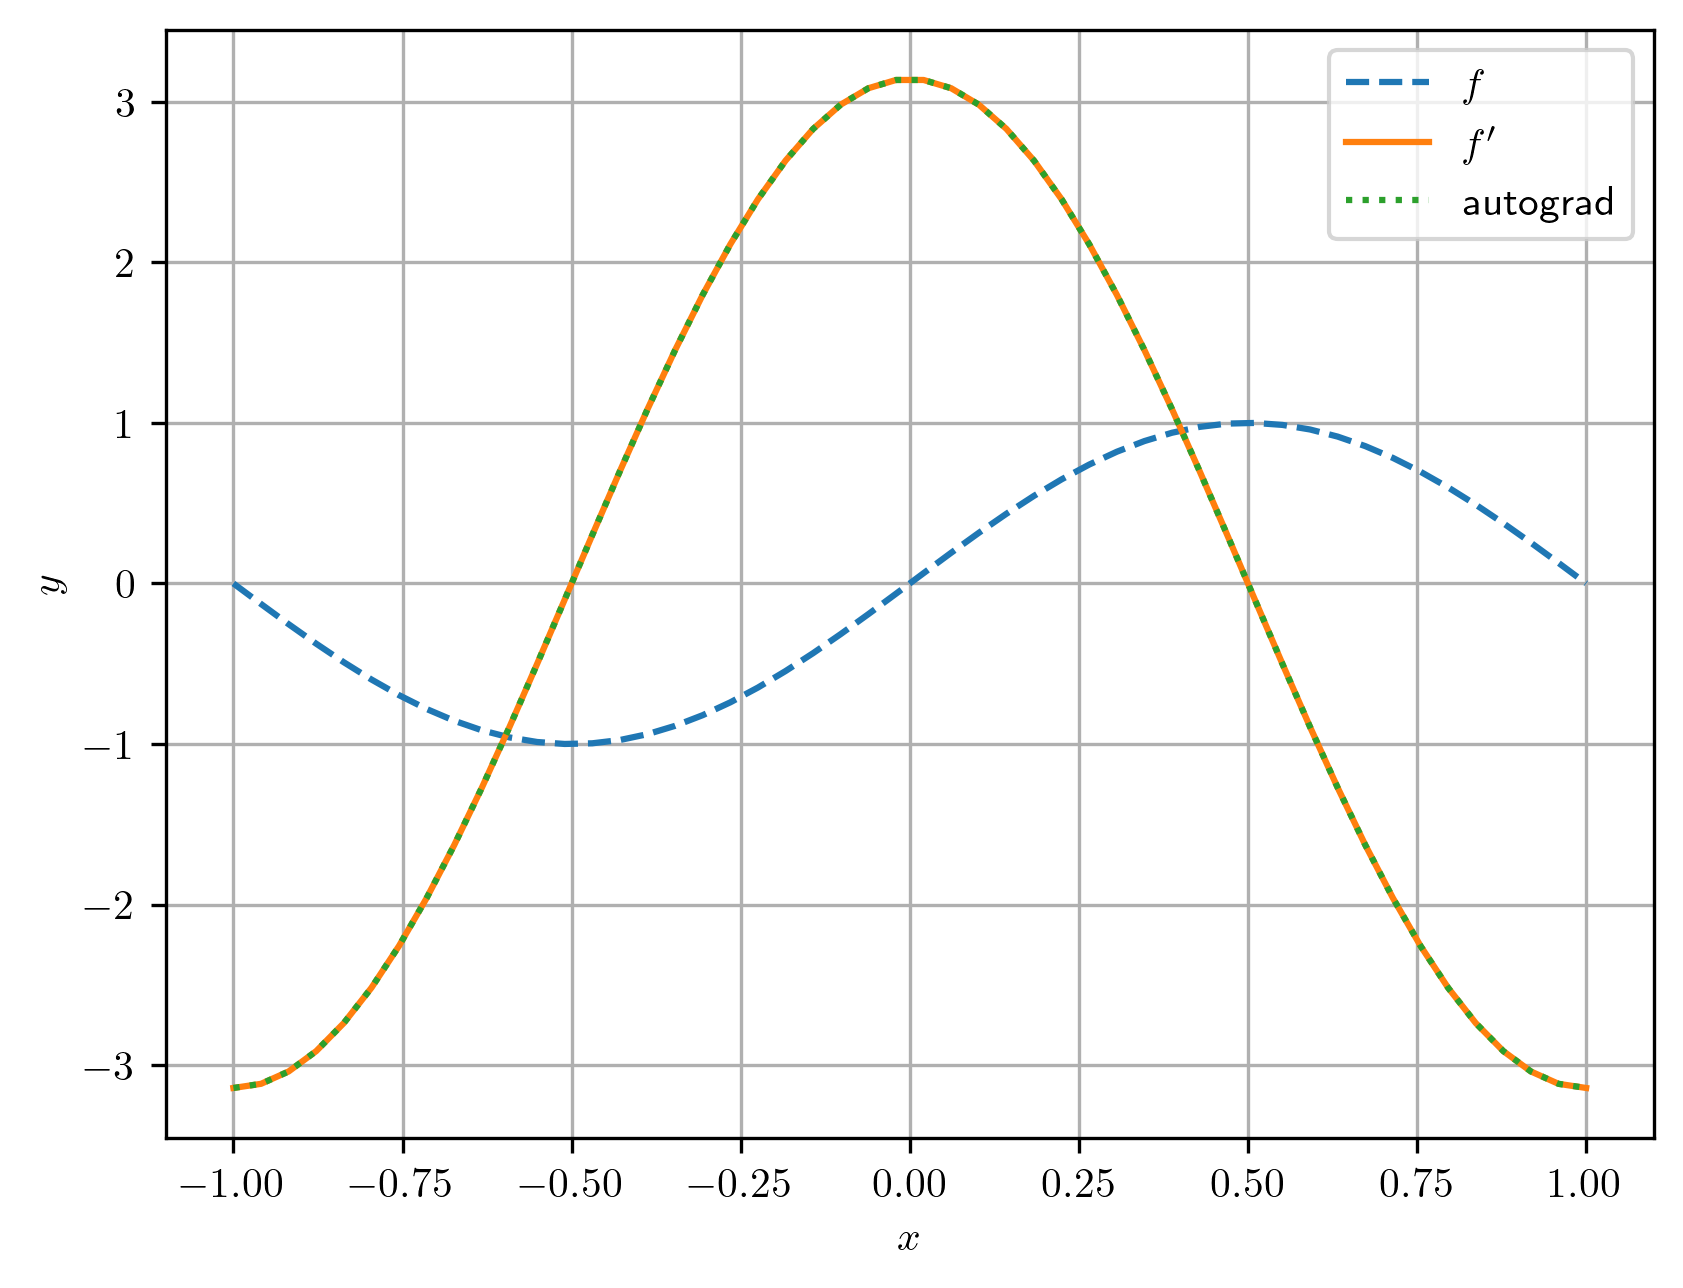
\includegraphics[width=0.7\textwidth]{./cap_interp/dados/fig_poliInterp/fig}
  \caption{Esboço do polinômio interpolador referente ao Exemplo \ref{cap_interp_sec_interpoli:ex:interpoli_intro}.}
  \label{cap_interp_sec_interpoli:fig:interpoli_intro}
\end{figure}

\begin{lstlisting}[caption=poliInterp.py]
import numpy as np
import numpy.linalg as npla

def poliInterp(x, y):
    # num. pts
    n = x.size
    # Vandermonde
    A = np.empty((n,n))
    for j in range(n):
        A[:,j] = x**(n-1-j)
    # coefs
    p = npla.solve(A, y)
    return p

# exemplo
x = np.array([-1., 0, 1])
y = np.array([-1., 1, 1/2])

# poli interp
p = poliInterp(x, y)

# verificação
print(np.polyval(p, x))
\end{lstlisting}
\end{ex}

\subsection{Exercícios}

\begin{exer}
  Obtenha o polinômio interpolador do conjunto de pontos $\{(-1, -1), (-0.5, 1), (1, 2)\}$.
\end{exer}
\begin{resp}
  $-1,\bar{6}x^2 + 1.5x + 2.1\bar{6}$
\end{resp}

\begin{exer}
  Obtenha o polinômio interpolador do conjunto de pontos $\{(-1, -1), (0, 1), (1, 1/2), (2, 1)\}$.
\end{exer}
\begin{resp}
  $0,58\bar{3}x^3 - 1,25x^2 + 0,1\bar{6}x + 1$. 
\end{resp}

\begin{exer}
  Obtenha o polinômio interpolador do conjunto de pontos $\{(-1,~-1), (0,~1), (1,~1/2), (2,~1), (2.5, 1)\}$.
\end{exer}
\begin{resp}
  $-0.26190476x^4  1.10714286x^3 -0.98809524x^2 -0.35714286x  1$.  
\end{resp}

\begin{exer}
  Considere a matriz de Vandermonde $V = [\pmb{x}^{n-j}]_{j=1}^{n}$, com $\pmb{x} = (x_1, x_2, \dotsc, x_n)$, sendo $x_i = (i-1)h$, $h=0.1$ e $i = 1, 2, \dotsc, n$. Compute o número de condicionamento de $V$ para $n=5, 10, 100$. De que forma os resultados obtidos impactam no problema de interpolação polinomial?
\end{exer}
\begin{resp}
  \begin{tabular}{ll}
    $n$ & $\kappa(V)$\\\hline
    $5$ & $1.03\E+4$\\
    $10$ & $2.57\E+7$\\
    $100$ & $9.11\E+109$\\\hline
  \end{tabular}
\end{resp}

\begin{exer}
  Aproxime a função $f(x) = \cos(x)$ por um polinômio interpolador $p$ no intervalo $[0, \pi]$. Escolhas pontos nesse intervalo de forma a obter $p$ que aproxime $f$ com boa precisão gráfica.
\end{exer}
\begin{resp}
  Dica: use os pontos $x_i = (i-1)\frac{\pi}{4}$, $i=1,2,3,4$.
\end{resp}

\section{Interpolação de Lagrange}\label{cap_interp_sec_lagrange}

\begin{flushleft}
  [[tag:revisar]]
\end{flushleft}

Interpolação de Lagrange\footnote{Joseph-Louis Lagrange, 1736 - 1813, matemático italiano. Fonte: \href{https://en.wikipedia.org/wiki/Joseph-Louis_Lagrange}{Wikipedia}.} é uma técnica para a computação do polinômio interpolador $p(x)$ de um conjunto de pontos $\{(x_i, y_i)\}_{i=1}^n$ dados. A ideia consiste em escrever o polinômio interpolador na forma
\begin{equation}
  p(x) = y_1L_1(x) + y_2L_2(x) + \cdots + y_nL_n(x),
\end{equation}
onde $L_i(x)$ é chamado de $i$-ésimo polinômio de Lagrange e é definido como o polinômio de grau $n-1$ que satisfaz
\begin{equation}
  L_i(x_j) = \left\{
    \begin{array}{ll}
      1 &, i=j\\
      0 &, i\neq j
    \end{array}
\right.
\end{equation}
Mais especificamente, temos que $L_i(x)$ tem raízes $\{x_1, \ldots, x_{i-1}, x_{i+1}, \ldots, x_n\}$ e, portanto, pode ser decomposto na forma
\begin{equation}
  L_i(x) = c_i(x-x_1)\cdots(x-x_{i-1})(x-x_i)\cdots(x-x_n).
\end{equation}
Além disso, como $L_i(x_i) = 1$, temos
\begin{equation}
  c_i = \frac{1}{(x_i-x_1)\cdots(x_i-x_{i-1})(x_i-x_i)\cdots(x_i-x_n)}.
\end{equation}
Assim sendo, podemos concluir que
\begin{equation}
  L_i(x) = \frac{(x-x_1)\cdots(x-x_{i-1})(x-x_{i+1})\cdots(x-x_n)}{(x_i-x_1)\cdots(x_i-x_{i-1})(x_i-x_{i+1})\cdots(x_i-x_n)}.
\end{equation}


\begin{ex}
  Consideremos o problema de encontrar o polinômio interpolador do conjunto de pontos $\{(-1,~-1), (0,~1), (1,~1/2)\}$. Como temos 3 pontos, o polinômio tem grau 2 e pode ser escrito na seguinte forma de Lagrange
  \begin{equation}
    p(x) = y_1L_1(x) + y_2L_2(x) + y_3L_3(x),
  \end{equation}
  onde $y_1 = -1$, $y_2 = 1$ e $y_3 = 1/2$. Os polinômios de Lagrange são dados por
  \begin{align}
    L_1(x) &= \frac{(x-x_2)(x-x_3)}{(x_1-x_2)(x_1-x_3)} = \frac{1}{2}x^2 - \frac{1}{2}x,\\
    L_2(x) &= \frac{(x-x_1)(x-x_3)}{(x_2-x_1)(x_2-x_3)} = -x^2 + 1,\\
    L_3(x) &= \frac{(x-x_1)(x-x_2)}{(x_3-x_1)(x_3-x_2)} = \frac{1}{2}x^2 + \frac{1}{2}x.\\
  \end{align}
  E, então, temos o polinômio interpolador
  \begin{equation}
    p(x) = -1,25x^2 + 0,75x + 1.
  \end{equation}

\ifisoctave
No \verb+GNU Octave+, podemos fazer as computações acima com o seguinte \href{https://github.com/phkonzen/notas/blob/master/src/MatematicaNumerica/cap_interp/dados/ex_interpoli_lagrange/ex_interpoli_lagrange.m}{código}:
\verbatiminput{./cap_interp/dados/ex_interpoli_lagrange/ex_interpoli_lagrange.m}
\fi
\end{ex}

\subsection{Aproximação de funções}

\begin{flushleft}
  [[tag:revisar]]
\end{flushleft}

Polinômio interpoladores podem ser usados para a aproximação de funções. Podemos aproximar uma dada função $f$ pelo polinômio interpolador de um conjunto de pontos selecionados $\{(x_i, y_i=f(x_i))\}_{i=1}^n$. De fato, o seguinte teorema nos fornece uma estimativa para o erro de uma tal interpolação.

\begin{teo}(\normalfont{Teorema de Lagrange})\label{teo:lagrange}
  Sejam dados uma função $f$ $n+1$-vezes continuamente diferenciável em um dado intervalo $[a, b]$ e $n$ pontos $\{x_i\}_{i=1}^n\subset [a, b]$. Então, o polinômio interpolador do conjunto de pontos $\{x_i, y_i=f(x_i)\}_{i=1}^n$ satisfaz
  \begin{equation}
    f(x) = p(x) + \frac{f^{(n+1)}(\xi)}{(n+1)!}(x-x_1)(x-x_2)\cdots (x-x_n).
  \end{equation}
\end{teo}
\begin{dem}
  \emconstrucao
\end{dem}

\begin{ex}\label{ex:interpoli_aprox}
  Considere o problema de aproxima $f(x) = \sen(x)$ pelo polinômio interpolador pelo conjunto de pontos $x_1=0$, $x_2=\pi/2$ e $x_3=\pi$. Isto, queremos determinar o polinômio $p(x)$ de grau $2$ que interpola os pontos $\{(0,0),~(\pi/2,~1),~(\pi,0)\}$. Usando a técnica de Lagrange, obtemos
  \begin{equation}
    p(x) = -0,41x^2 + 1,3x,
  \end{equation}
com seus coeficientes arredondados para dois dígitos significativos. A Figura \ref{fig:interpoli_aprox} mostra os esboços da função $f(x)=\sen(x)$, dos pontos dados e do polinômio interpolador $p(x)$.

\begin{figure}[h!]
  \centering
  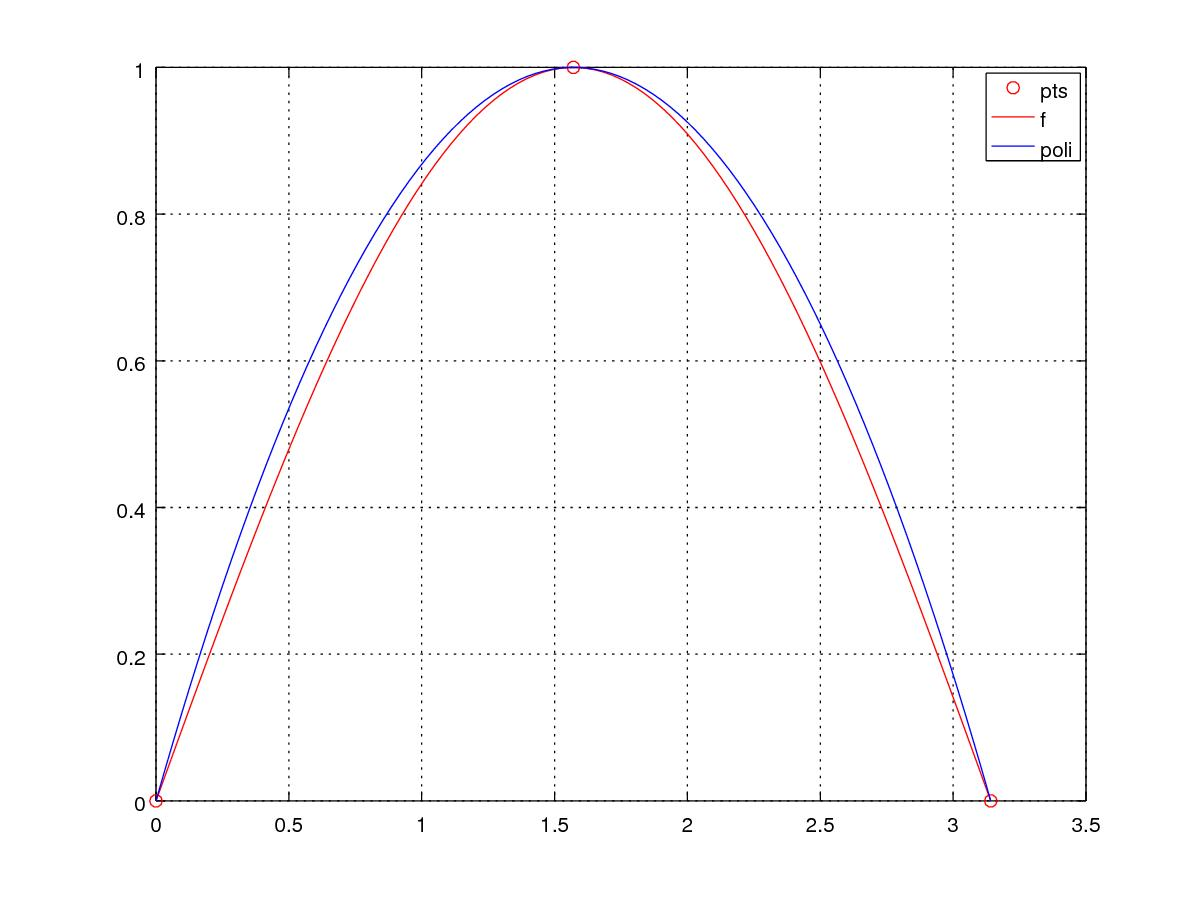
\includegraphics[width=0.7\textwidth]{./cap_interp/dados/ex_interpoli_aprox/fig_interpoli_aprox}
  \caption{Esboços dos gráficos da função, dos pontos e do polinômio interpolador computado no Exemplo \ref{ex:interpoli_aprox}.}
  \label{fig:interpoli_aprox}
\end{figure}

\ifisoctave
No \verb+GNU Octave+, podemos fazer as computações acima com o seguinte \href{https://github.com/phkonzen/notas/blob/master/src/MatematicaNumerica/cap_interp/dados/ex_interpoli_aprox/ex_interpoli_aprox.m}{código}:
\verbatiminput{./cap_interp/dados/ex_interpoli_aprox/ex_interpoli_aprox.m}
\fi
\end{ex}

\subsection*{Exercícios}

\begin{flushleft}
  [[tag:revisar]]
\end{flushleft}

\begin{exer}
  Use a técnica de interpolação de Lagrange para encontrar o polinômio interpolador que aproxima a função$f(x)=e^{x}$ pelos pontos $x_1=0$, $x_2=1$, $x_3=1,5$ e $x_4=2$.
\end{exer}
\begin{resp}
\ifisoctave
\href{https://github.com/phkonzen/notas/blob/master/src/MatematicaNumerica/cap_interp/dados/exer_interpoli_aprox1/exer_interpoli_aprox1.m}{Código}.
\fi
$0,54x^3 - 0,15x^2 + 1,3x + 1$.
\end{resp}

\section{Diferenças divididas de Newton}\label{cap_interp_difdiv}

\begin{flushleft}
  [[tag:revisar]]
\end{flushleft}

Dado um conjunto de pontos $\{(x_i, y_i)\}_{i=1}^n$, o método das diferenças divididas de Newton\footnote{Carl Gustav Jacob Jacobi, 1804 - 1851, matemático alemão. Fonte: \href{https://en.wikipedia.org/wiki/Carl_Gustav_Jacob_Jacobi}{Wikipedia}.} busca determinar o polinômio interpolar deste conjunto de pontos na forma
\begin{align}
  p(x) &= a_1 + a_2(x-x_1) + a_3(x-x_1)(x-x_2)\\
       &+ \cdots + a_{n}(x-x_1)\cdot \cdots \cdot (x-x_{n-1}).
\end{align}

Por uma abordagem direta, temos que $p(x_i)=y_i$, $i=1, 2, \dotsc, n$, o que nos leva ao seguinte sistema triangular inferior
\begin{align}
  a_1 &= y_1, \\
  a_1 + a_2(x_2-x_1) &= y_2, \\
  a_1 + a_2(x_3-x_1) + a_3(x_3-x_1)(x_3-x_2) &= y_3, \\
  &\vdots\\
  a_1 + a_2(x_n-x_1) + \cdots + a_{n}(x_n-x_1)\cdot\cdots\cdot(x_n-x_{n-1}) &= y_n.
\end{align}
Entretanto, existe uma forma mais eficiente de se determinar os coeficientes $a_i$, $i=1, 2, \dotsc, n$.

Denotemos por $p[x_j, x_{j+1}, \dotsc, x_{k}](x)$ o polinômio interpolador do conjunto de pontos $\{(x_i, y_i)\}_{i=j}^k$. Então, temos a seguinte recursão
\begin{equation} \label{eq:interp_parc1}
  p[x_j] = y_j,\quad j=1, 2, \dotsc, n,
\end{equation}
e
\begin{align}
  &p[x_j, x_{j+1}, \ldots, x_k](x) \nonumber\\
  &= \frac{(x-x_j)p[x_{j+1},\dotsc,x_k](x)-(x-x_k)p[x_j,\dotsc,x_{k-1}](x)}{x_k-x_j},\label{eq:interp_parc2}
\end{align}
para todo $n\geq k > j \geq 1$. De fato, \eqref{eq:interp_parc1} é trivial. Agora, denotando por $r(x)$ o lado direito da equação \eqref{eq:interp_parc2}, vemos que $r(x)$ tem grau menor ou igual a $k-j$, o mesmo de $p[x_j, x_{j+1}, \ldots, x_k](x)$. Desta forma, para mostrar \eqref{eq:interp_parc2}, basta verificarmos que $r(x)$ interpola o conjunto de pontos $\{(x_i, y_i)\}_{i=j}^k$. O que de fato ocorre:
\begin{align}
  r(x_j) &= \frac{-(x_j-x_k)y_j}{x_k-x_j} = y_j,\\
  r(x_{l}) &= \frac{(x_l-x_j)y_l-(x_l-x_k)y_l}{x_k-x_j}=y_l,~l=j+1,\dotsc,k-1,\\
  r(x_k) &= \frac{(x_k-x_j)y_k}{x_k-x_j}=y_k.
\end{align}
Logo, pela unicidade do polinômio interpolador, temos demonstrado \eqref{eq:interp_parc2}.

Observando que o polinômio interpolador $p(x)$ é igual a $p[x_1,\dotsc,x_n](x)$, temos que \eqref{eq:interp_parc1}-\eqref{eq:interp_parc2} nos fornece uma forma de computar $p(x)$ recursivamente\footnote{De fato, o método de Neville consistem em computar $p(x)$ por esta recursão.}. Além disso, observemos que $p[x_j,\dotsc,x_{k-1}](x)$ e $p[x_j,\dotsc,x_k]$ diferem por um polinômio de grau $k-j$ com zeros $x_j$, $x_{j+1}$, ..., $x_{k-1}$. Logo, temos
\begin{align}
  p[x_j,\dotsc,x_k](x) &= p[x_j,\dotsc,x_{k-1}](x) \nonumber \\
                       &+ f[x_j,\dotsc,x_k](x-x_j)\cdot\cdots\cdot(x-x_{k-1}),
\end{align}
onde $f[x_j,\dotsc,x_k]$ são coeficientes a determinar. Ainda, tomando $p[x_i]=f[x_i]$, temos
\begin{align}
  p[x_j,\dotsc,x_k](x) &= f[x_j] + f[x_j,x_{j+1}](x-x_j) \nonumber \\
                       &+ f[x_j,\dotsc,x_k](x-x_j)\cdot\cdots\cdot(x-x_{k-1}).
\end{align}
Por fim, a recursão \eqref{eq:interp_parc1}-\eqref{eq:interp_parc2} nos mostra que as diferenças divididas Newton podem ser obtidas de
\begin{align}
  &f[x_j] = y_j,\quad j=1,2,\dotsc,n,\label{eq:interp_difdiv1}\\
  &f[x_j,\dotsc,x_k] = \frac{f[x_{j+1},\dotsc,x_k]-f[x_j,\dotsc,x_{k-1}]}{x_k-x_j},\label{eq:interp_difdiv2}
\end{align}
para todo $n\geq k>j\geq 1$. E, temos o polinômio interpolador do conjunto de pontos $\{(x_i,y_i)\}_{i=1}^n$ dado por
\begin{align}\label{eq:interpoli_Newton}
  p[x_1,\dotsc,x_n](x) &= f[x_1] + f[x_1,x_2](x-x_1) \nonumber \\
                       &+\cdots + f[x_1,\dotsc,x_n](x-x_1)\cdot\cdots\cdot(x-x_n).  
\end{align}

\begin{obs}
  A recursão \eqref{eq:interp_difdiv1}-\eqref{eq:interp_difdiv2} pode ser adequadamente organizada em uma matriz da forma
  \begin{equation}
    \begin{bmatrix}
      \pmb{f[x_1]} & 0 & 0 & \ldots & 0 \\
      f[x_2] & \pmb{f[x_1,x_2]} & 0 & \ldots & 0 \\
      f[x_3] & f[x_2,x_3] & \pmb{f[x_1,x_2,x_3]} & \ldots & 0\\
      \vdots & \vdots & \vdots & \ldots & \vdots \\
      f[x_n] & f[x_{n-1},x_{n}] & f[x_{n-2},x_{n-1},x_n] & \ldots & \pmb{f[x_1,x_2,\dotsc,x_n]}
    \end{bmatrix}
  \end{equation}
onde os elementos da diagonal correspondem aos coeficientes do polinômio interpolador na forma \eqref{eq:interpoli_Newton}.
\end{obs}


\begin{ex}
  Consideremos o problema de encontrar o polinômio interpolador do conjunto de pontos $\{(-1,~-1), (0,~1), (1,~1/2)\}$. Usando o método das diferenças divididas de Newton, escrevemos o polinômio na forma
  \begin{equation}
    p(x) = f[x_1] + f[x_1,x_2](x-x_1) + f[x_1,x_2,x_3](x-x_1)(x-x_2).
  \end{equation}
  Então, computamos seus coeficientes pela recursão \eqref{eq:interp_difdiv1}-\eqref{eq:interp_difdiv2}. Ou seja, temos
  \begin{equation}
    f[x_1]=-1,~f[x_2]=1,~f[x_3]=1/2.
  \end{equation}
  Daí, segue
  \begin{align}
    f[x_1,x_2] &= \frac{f[x_2]-f[x_1]}{x_2-x_1} = 2\\
    f[x_2,x_3] &= \frac{f[x_3]-f[x_2]}{x_3-x_2} = -\frac{1}{2}\\
  \end{align}
  e, então,
  \begin{equation}
    f[x_1,x_2,x_3] = \frac{f[x_2,x_3]-f[x_1,x_2]}{x_3-x_1}=-1,25.
  \end{equation}
  Logo, o polinômio interpolador é
  \begin{equation}
    p(x) = 0,5 + 2(x+1) - 1,25(x+1)(x-1),
  \end{equation}
  ou, equivalentemente,
  \begin{equation}
    p(x) = -1,25x^2 + 0,75x + 1.
  \end{equation}

\ifisoctave
No \verb+GNU Octave+, podemos fazer as computações acima com o seguinte \href{https://github.com/phkonzen/notas/blob/master/src/MatematicaNumerica/cap_interp/dados/ex_interpoli_difdiv/ex_interpoli_difdiv.m}{código}:
\verbatiminput{./cap_interp/dados/ex_interpoli_difdiv/ex_interpoli_difdiv.m}
\fi
\end{ex}

\subsection*{Exercícios}

\begin{flushleft}
  [[tag:revisar]]
\end{flushleft}

\begin{exer}\label{exer_interpoli_difdiv1}
  Use o método das diferenças divididas de Newton para encontrar o polinômio interpolador que aproxima a função $f(x)=e^{x}$ pelos pontos $x_1=0$, $x_2=1$, $x_3=1,5$ e $x_4=2$.
\end{exer}
\begin{resp}
\ifisoctave
\href{https://github.com/phkonzen/notas/blob/master/src/MatematicaNumerica/cap_interp/dados/exer_interpoli_dfidiv1/exer_interpoli_difdiv1.m}{Código}.
\fi
$0,54x^3 - 0,15x^2 + 1,3x + 1$.
\end{resp}


\section{Spline cúbico}\label{cap_interp_splines}

\begin{flushleft}
  [[tag:revisar]]
\end{flushleft}

Dado um conjunto de pontos $\{(x_i,y_i)\}_{i=1}^n$, um spline cúbico é uma função duas vezes continuamente diferenciável da forma
\begin{equation}
  \begin{small}
    s(x)\!=\!\left\{
      \begin{array}{ll}
        \!s_{11}(x-x_1)^3 + s_{12}(x-x_1)^2 + s_{13}(x-x_1) + s_{14} &,x_1\!\leq\!x\!<\!x_2,\\
        \!s_{21}(x-x_2)^3 + s_{22}(x-x_2)^2 + s_{23}(x-x_2) + s_{24} &,x_2\!\leq\!x\!<\!x_3,\\
                                                                   &, \vdots \\
        \!s_{n-1,1}(x-x_2)^3\!+\!s_{n-1,2}(x-x_2)^2\!+\!s_{n-1,3}(x-x_2)\!+\!s_{n-1,4}\!&,x_{n-1}\!\leq\!x\!\leq\!x_n.
      \end{array}
    \right.
  \end{small}
\end{equation}
que satisfaz as seguintes propriedades
\begin{enumerate}
\item $s(x_i) = y_i$ para $i=1, 2, \dotsc, n$,
\item $s_j(x_j) = s_{j+1}(x_j)$ para todo $j=1,2,\dotsc,n-2$,
\item $s_j'(x_j) = s_{j+1}'(x_j)$ para todo $j=1,2,\dotsc,n-2$,  
\item $s_j''(x_j) = s_{j+1}''(x_j)$ para todo $j=1,2,\dotsc,n-2$.
\end{enumerate}

Observemos que o spline tem $4(n-1)$ coeficientes a determinar, enquanto que as condições acima nos fornecem $4n-6$ equações. Assim sendo, nota-se a determinação de um spline requer ainda 2 condições. Conforme a escolha destas condições, diferentes splines cúbicos são computados.

\subsection{Spline {\it Not-a-knot}}

\begin{flushleft}
  [[tag:revisar]]
\end{flushleft}

A condição {\it not-a-knot} exige que o spline cúbico tenha derivada terceira contínua nos pontos $x_2$ e $x_{n-1}$, i.e.
\begin{equation}
  s_1'''(x_2) = s_2'''(x_2)\quad\text{e}\quad s_{n-2}'''(x_{n-1}) = s_{n-1}'''(x_{n-1}).
\end{equation}

\begin{ex}\label{ex:interp_spline_nak}
  Consideremos o problema de aproximar a função $f(x)=\sen(x)$ pelo spline cúbico {\it not-a-knot} com pontos suporte $x_1=0$, $x_2=\pi/3$, $x_3=\pi/6$ e $x_4=\pi/2$. Na Figura \ref{fig:interp_spline_nak} temos os esboços de $f$ e do spline cúbico computado.

  \begin{figure}[h!]
    \centering
    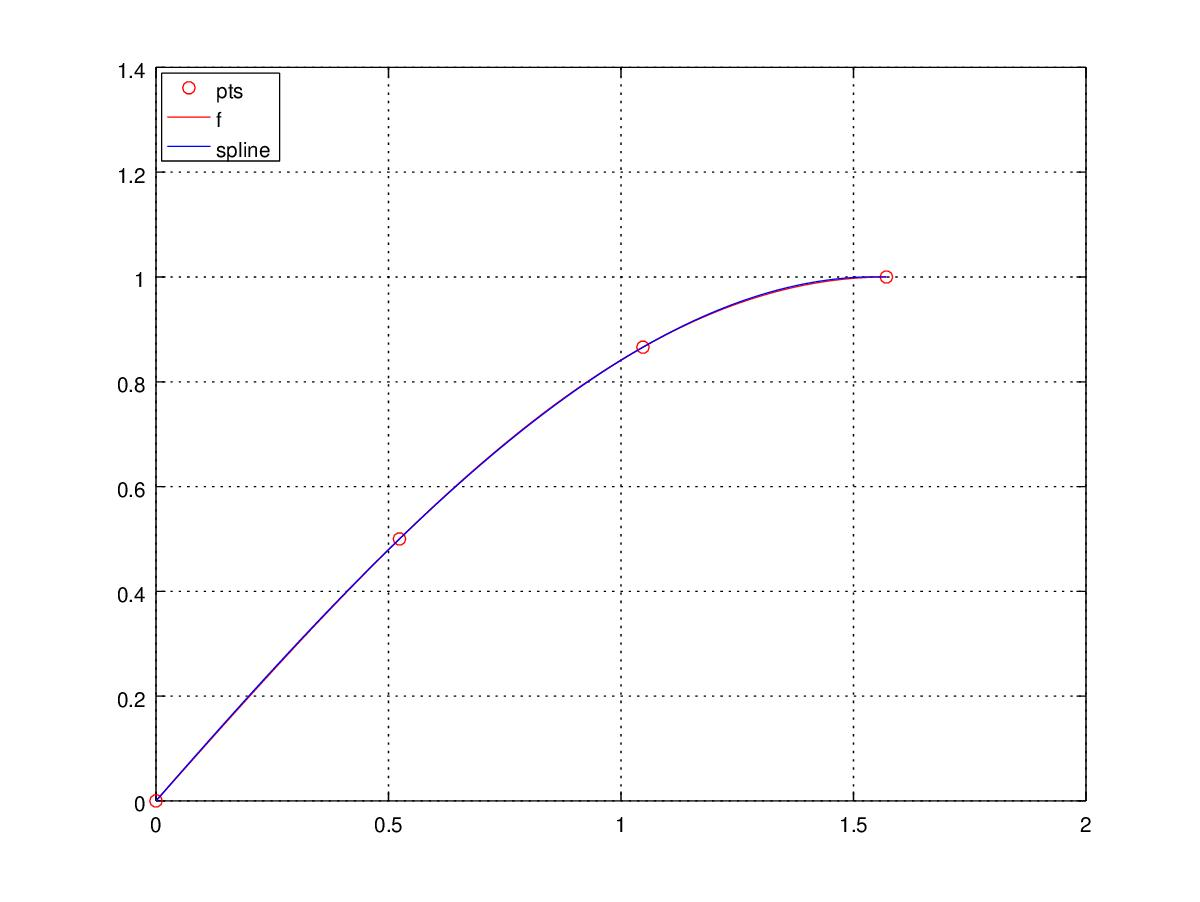
\includegraphics[width=0.7\textwidth]{./cap_interp/dados/ex_interp_spline_nak/fig_interp_spline_nak}
    \caption{Esboço dos gráficos da função $f(x)=\sen(x)$ e do spline cúbico computado no Exemplo \ref{ex:interp_spline_nak}.}
    \label{fig:interp_spline_nak}
  \end{figure}

\ifisoctave
No \verb+GNU Octave+, podemos fazer as computações acima com o seguinte \href{https://github.com/phkonzen/notas/blob/master/src/MatematicaNumerica/cap_interp/dados/ex_interp_spline_nak/ex_interp_spline_nak.m}{código}:
\verbatiminput{./cap_interp/dados/ex_interp_spline_nak/ex_interp_spline_nak.m}
\fi
\end{ex}

\subsection{Spline fixado}

\begin{flushleft}
  [[tag:revisar]]
\end{flushleft}

Os splines cúbicos fixados são obtidos com as condições de fronteira
\begin{equation}
  s'(x_1)=y_1',\quad\text{e}\quad s'(x_n)=y_n',
\end{equation}
onde $y_1'$ e $y_n'$ são escalares dados. Quando usamos splines para aproximarmos uma dada função $f$, usualmente, escolhemos $y_1'=f'(x_1)$ e $y_n'=f'(x_n)$.

\begin{ex}\label{ex:interp_spline_fixado}
  Consideremos o problema de aproximar a função $f(x)=\sen(x)$ pelo spline cúbico fixado com pontos suporte $x_1=0$, $x_2=\pi/3$, $x_3=\pi/6$ e $x_4=\pi/2$. Na Figura \ref{fig:interp_spline_fixado} temos os esboços de $f$ e do spline cúbico computado.

  \begin{figure}[h!]
    \centering
    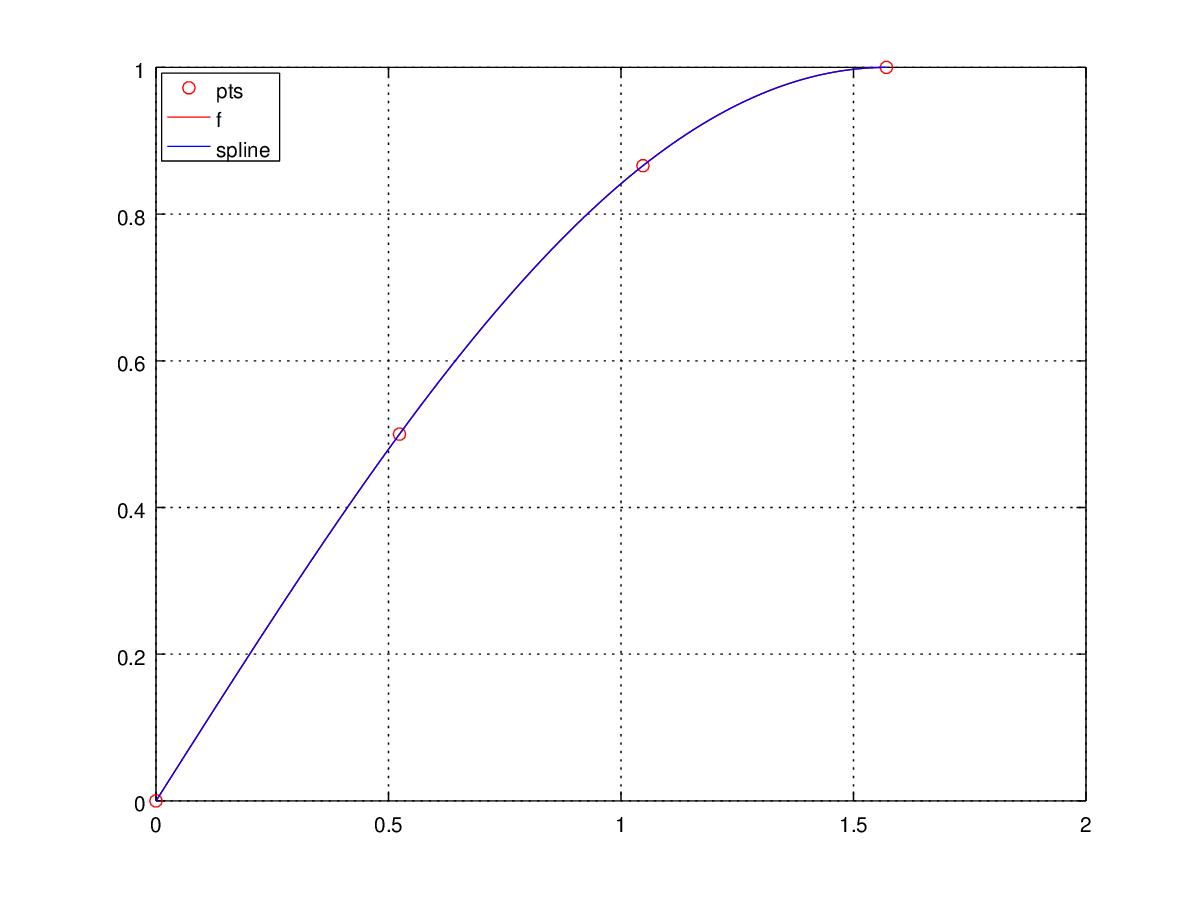
\includegraphics[width=0.7\textwidth]{./cap_interp/dados/ex_interp_spline_fixado/fig_interp_spline_fixado}
    \caption{Esboço dos gráficos da função $f(x)=\sen(x)$ e do spline cúbico computado no Exemplo \ref{ex:interp_spline_fixado}.}
    \label{fig:interp_spline_fixado}
  \end{figure}

\ifisoctave
No \verb+GNU Octave+, podemos fazer as computações acima com o seguinte \href{https://github.com/phkonzen/notas/blob/master/src/MatematicaNumerica/cap_interp/dados/ex_interp_spline_fixado/ex_interp_spline_fixado.m}{código}:
\verbatiminput{./cap_interp/dados/ex_interp_spline_fixado/ex_interp_spline_fixado.m}
\fi
\end{ex}

\subsection*{Exercícios}

\begin{flushleft}
  [[tag:construcao]]
\end{flushleft}

%%Este trabalho está licenciado sob a Licença Atribuição-CompartilhaIgual 4.0 Internacional Creative Commons. Para visualizar uma cópia desta licença, visite http://creativecommons.org/licenses/by-sa/4.0/ ou mande uma carta para Creative Commons, PO Box 1866, Mountain View, CA 94042, USA.

\chapter{Aproximação por mínimos quadrados}\label{cap_ajuste}
\thispagestyle{fancy}

\begin{flushleft}
  [[tag:revisar]]
\end{flushleft}

\section{Problemas lineares}\label{cap_ajuste_sec_prob_lin}

\begin{flushleft}
  [[tag:revisar]]
\end{flushleft}

Dado um conjunto de $n$ pontos $\{(x_i,y_i)\}_{i=1}^n$, $x_i\neq x_j$ para $i\neq j$, e uma família de $m \leq n$ funções $\{f_i(x)\}_{i=1}^m$, o problema linear de aproximação por mínimos quadrados consiste em determinar os $m$ coeficientes $\{c_i\}_{i=1}^m$ tal que a função
\begin{align}    
  f(x;c) &= \sum_{j=1}^m c_jf_j(x) \\
         &= c_1f_1(x) + c_2f_2(x) + c_3f_3(x) + \cdots + c_mf_m(x)
\end{align}
aproxime o conjunto de pontos dados no sentido de mínimos quadrados, i.e. o vetor dos coeficientes $c = (c_1, c_2, \dotsc, c_m)$ é solução do seguinte problema linear de minimização
\begin{equation}
  \min_{c} \left\{E:= \sum_{i=1}^n (y_i - f(x_i;c))^2\right\}.
\end{equation}

A fim de trabalharmos com uma notação mais compacta, definimos o resíduo $r(c) = (r_1(c), r_2(c), \dotsc, r_n(c))$, onde $r_i(c) := y_i - f(x_i)$ e $c = (c_1, c_2, \dotsc, c_m)$. Com esta notação, o problema de mínimos quadrados se resume a resolver
\begin{equation}\label{eq:pmq}
  \min_{c} \{E := \|r(c)\|_2^2\}.
\end{equation}

\subsection{Método das equações normais}

\begin{flushleft}
  [[tag:revisar]]
\end{flushleft}

A fim de resolver o problema de mínimos quadrados~\eqref{eq:pmq}, observamos que o erro quadrático
\begin{align}
  E &= \|r(c)\|_2^2 \\
    &= \sum_{i=1}^n r_i(c)^2 \\
    &= \sum_{i=1}^n \left(y_i - f(x_i;c)\right)^2 \\
    &= \sum_{i=1}^n \left(y_i - \sum_{j=1}^m c_jf_j(x_i)\right)^2 \\
    &= \|y - Ac\|_2^2,
\end{align}
onde $y = (y_1, y_2, \dotsc, y_n)$ e
\begin{equation}
  A :=
  \begin{bmatrix}
    f_1(x_1) & f_2(x_1) & \cdots & f_m(x_1) \\
    f_1(x_2) & f_2(x_2) & \cdots & f_m(x_2) \\
    \vdots & \vdots & \vdots & \vdots \\
    f_1(x_n) & f_2(x_n) & \cdots & f_m(x_n)
  \end{bmatrix}.
\end{equation}

Os parâmetros $c_j$ que minimizam o erro $E$ são solução do seguinte sistema de equações
\begin{equation}
  \frac{\p E}{\p c_j} = 2\sum_{i=0}^n r_i(c)\frac{\p}{\p c_j}r_i(c) = 0,
\end{equation}
onde $j=1, 2, \dotsc, m$. Ou, em uma notação mais apropriada,
\begin{align}
  \nabla_c E = 0 &\Leftrightarrow A^Tr(c) = 0\\
  &\Leftrightarrow A^T(y - Ac) = 0\\
  &\Leftrightarrow A^TAc = A^Ty.
\end{align}

Portanto, o problema linear de mínimos quadrados se resume em resolver as chamadas \emph{equações normais}\index{equações normais}
\begin{equation}\label{eq:equacoes_normais}
  A^TAc= A^Ty.
\end{equation}

Logo, o problema linear de mínimos quadrados~\eqref{eq:pmq} reduz-se a resolver o sistema linear \eqref{eq:equacoes_normais} para $c$. Isto nos leva a questão de verificar se $A^TA$ é invertível. De sorte, da disciplina de álgebra linear temos o seguinte teorema.

\begin{teo}
  A matriz $A^TA$ é positiva definida se, e somente se, as colunas de $A$ são linearmente independentes (i.e. $\text{posto}(A)=n$).
\end{teo}
\begin{dem}
  Se as colunas de $A$ são linearmente independentes, então $x\neq 0$ implica $Ax\neq 0$ e, equivalentemente, $x^TA^T\neq 0$. Portanto, $x\neq 0$ implica $x^TA^TAx = \|Ax\|_2^2 > 0$, o que mostra que $A^TA$ é positiva definida.

  Suponhamos, agora, que as colunas de $A$ não são linearmente independentes. Então, existe $x_0\neq 0$ tal que $Ax_0 = 0$. Mas, então, $x_0^TA^TAx_0=0$, o que mostra que $A^TA$ não é positiva definida. 
\end{dem}

Este teorema nos fornece uma condição suficiente para a existência (e unicidade) de solução do problema linear de mínimos quadrados. Mais especificamente, se as colunas da matriz $A$ são linearmente independentes, então os coeficientes da função $f(x)$ que melhor ajustam os pontos dados são
\begin{equation}
  c = (A^TA)^{-1}A^Ty.
\end{equation}

\begin{ex}\normalfont{(Ajuste de polinômios)}\label{ex:ajuste_de_polinomios}
  Considere o problema de ajustar o conjunto de pontos
  \begin{center}
    \begin{tabular}{l|rrrr}
      $i$ & $1$ & $2$ & $3$ & $4$ \\\hline
      $x_i$ & $-1$ & $0$ & $1$ & $1,5$\\
      $y_i$ & $1,2$ & $-0,1$ & $0,7$ & $2,4$\\\hline
    \end{tabular}
  \end{center}
  por um polinômio quadrático da forma
  \begin{equation}
    p(x) = p_1x^2 + p_2x + p_3
  \end{equation}
  no sentido de mínimos quadrados.  

  \begin{figure}[h]
    \centering
    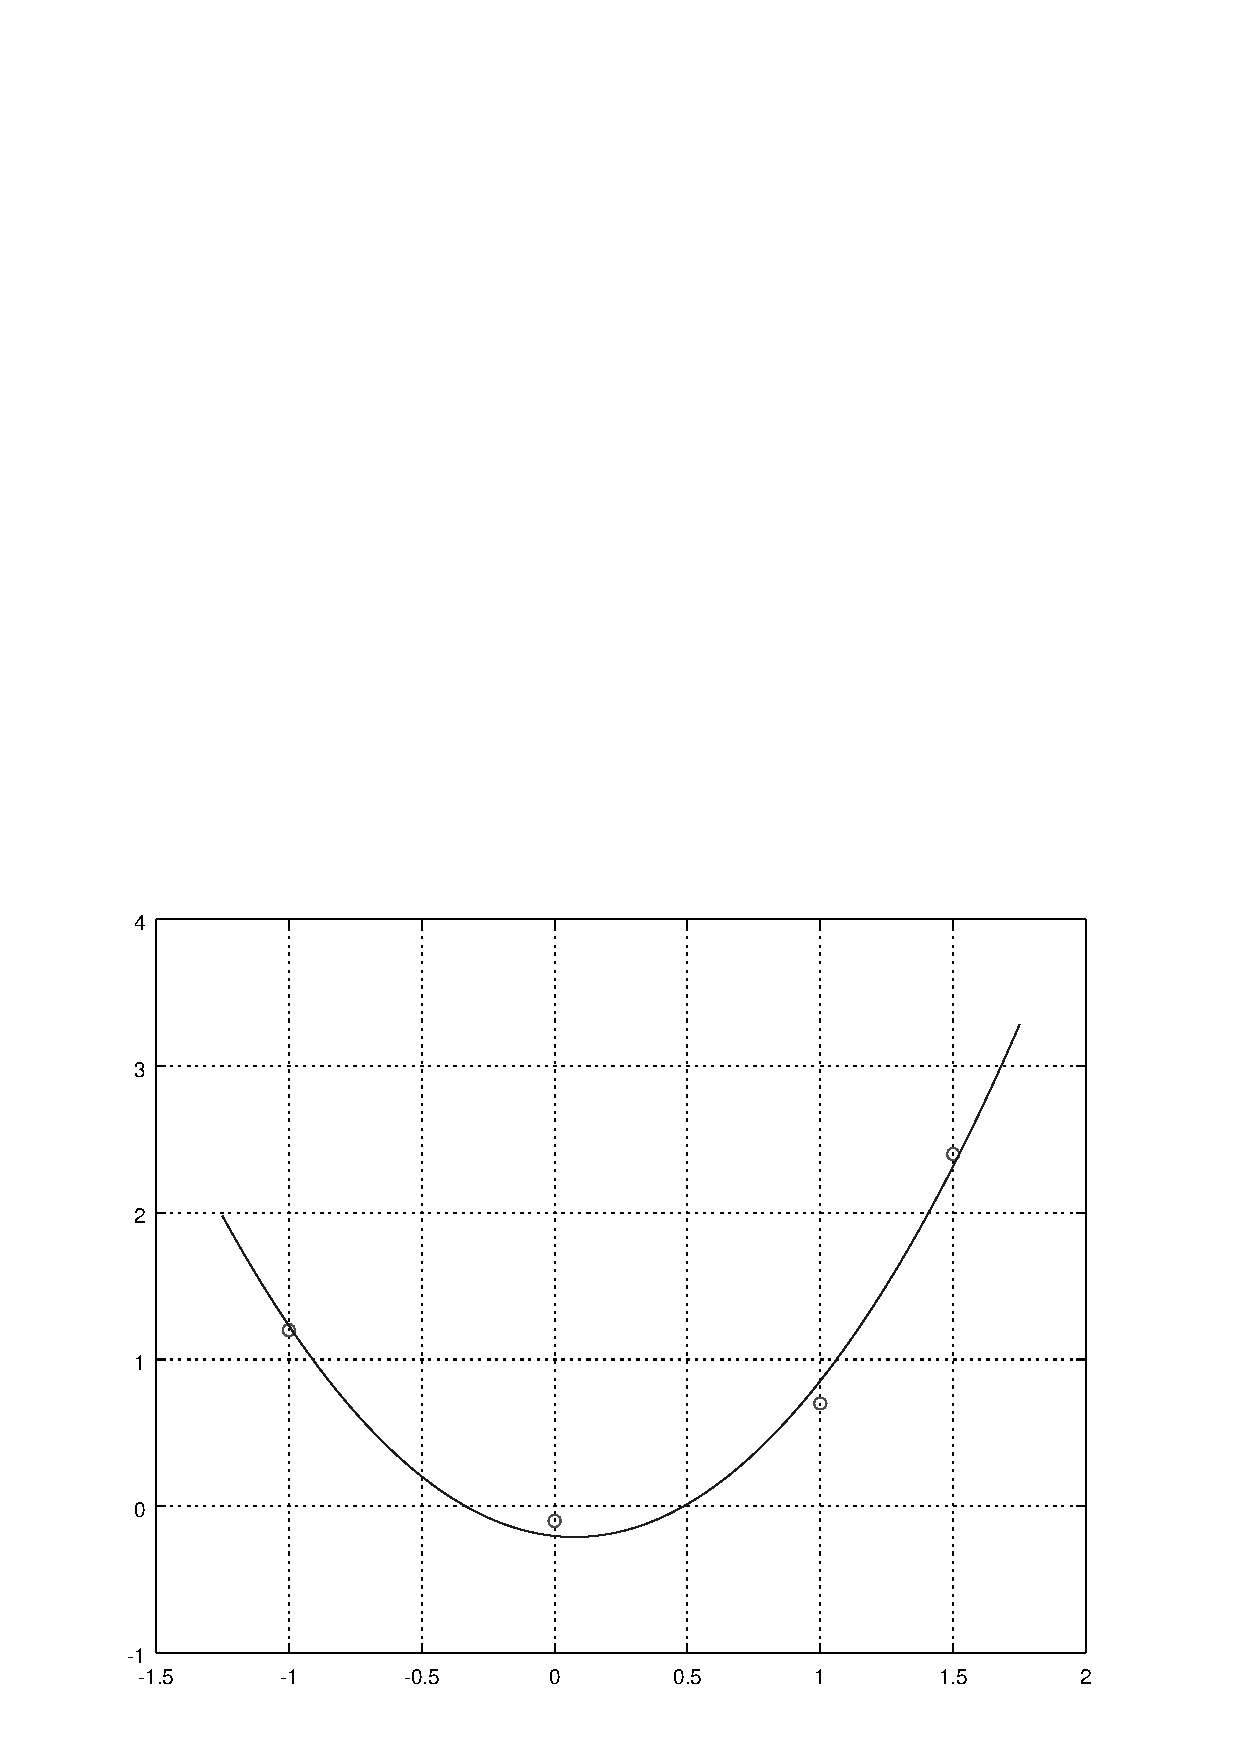
\includegraphics[width=\textwidth]{cap_ajuste/dados/ex_mq_poli/ex_mq_poli}
    \caption{Esboço do polinômio ajustado no Exemplo~\ref{ex:ajuste_de_polinomios}.}
    \label{fig:ex_mq_poli}
  \end{figure}
  
  
  Neste caso, a família de funções do problema de mínimos quadrados é $f_1(x) = x^2$, $f_2(x) = x$ e $f_3(x) = 1$. Assim sendo, os coeficientes $p = (p_1, p_2, p_3)$ são solução do seguinte sistema linear
  \begin{equation}\label{eq:aux3_md}
    A^TAp = A^Ty,
  \end{equation}
  onde $y = (y_1, y_2, y_3)$ e
  \begin{equation}
    A :=
    \begin{bmatrix}
      x_1^2 & x_1 & 1 \\
      x_2^2 & x_2 & 1 \\
      x_3^2 & x_3 & 1 \\
      x_4^2 & x_4 & 1
    \end{bmatrix}.
  \end{equation}
  Emfim, resolvendo as equações normais~\eqref{eq:aux3_md}, obtemos
  \begin{equation}
    p(x) = 1,25x^2 -0,188x - 0,203.
  \end{equation}
  A Figura~\ref{fig:ex_mq_poli} mostra um esboço dos pontos (em vermelho) e do polinômio ajustado (em azul).
  
%   \ifisoctave
%   Os coeficientes e um esboço do polinômio ajustado podem ser obtidos no \verb+GNU Octave+ com o seguinte código:
% \begin{verbatim}
% #pontos
% x = [-1 0 1 1.5]';
% y = [1.2, -0.1, 0.7, 2.4]';

% #resol. as eqs. normais
% A = [x.^2 x.^1 x.^0];
% p = inv(A'*A)*A'*y

% #esboco do pol. ajustado
% xx = linspace(-1.25,1.75);
% plot(x,y,'ro',...
%      xx,polyval(p,xx));grid
% \end{verbatim}
%   \fi
  
\end{ex}


\begin{ex}\normalfont{(Ajuste de curvas)}\label{ex:ajuste_de_curvas}
  Consideremos o mesmo conjunto de pontos do exemplo anterior (Exemplo~\ref{ex:ajuste_de_polinomios}). Aqui, vamos ajustar uma curva da forma
  \begin{equation}
    f(x) = c_1\sen(x) + c_2\cos(x) + c_3
  \end{equation}
no sentido de mínimos quadrados. Para tanto, formamos a matriz
\begin{equation}
  A :=
  \begin{bmatrix}
    \sen(x_1) & \cos(x_1) & 1 \\
    \sen(x_2) & \cos(x_2) & 1 \\
    \sen(x_3) & \cos(x_3) & 1 \\
    \sen(x_4) & \cos(x_4) & 1
  \end{bmatrix}
\end{equation}
  e, então, resolvemos as equações normais $A^TAc = A^Ty$ para o vetor de coeficientes $c=(c_1, c_2)$. Fazendo isso, obtemos $c_1=-0,198$, $c_2=-2,906$ e $c_3=2,662$. A Figura~\ref{fig:ex_ajuste_de_curvas} mostra um esboço da curva ajustada (linha azul) aos pontos dados (círculos vermelhos).

  \begin{figure}[h]
    \centering
    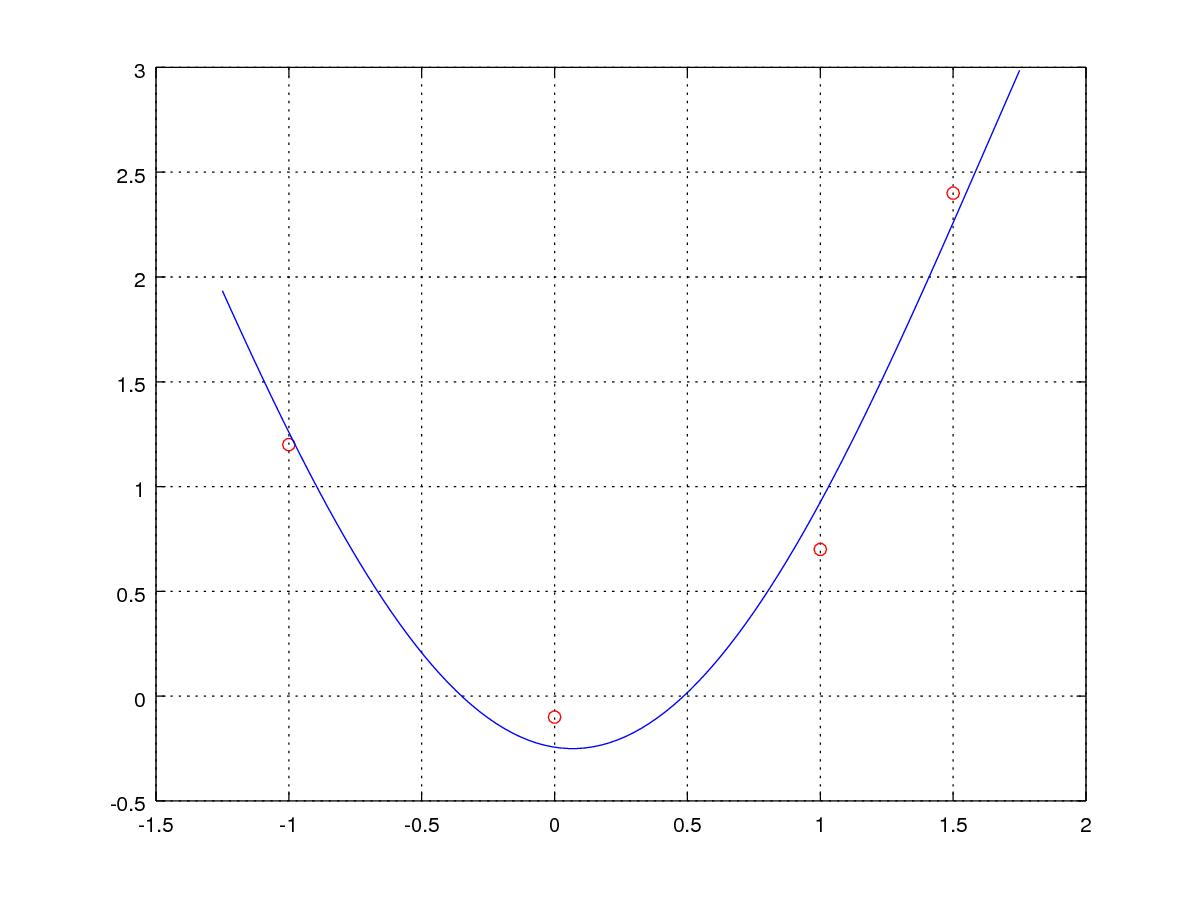
\includegraphics[width=\textwidth]{cap_ajuste/dados/ex_mq_curvas/ex_mq_curvas}
    \caption{Esboço da curva ajustada no Exemplo~\ref{ex:ajuste_de_curvas}.}
    \label{fig:ex_ajuste_de_curvas}
  \end{figure}

% \ifisoctave
% Os coeficientes e um esboço do polinômio ajustado podem ser obtidos no \verb+GNU Octave+ com o seguinte código:
% \begin{verbatim}
% #pontos
% x = [-1 0 1 1.5]';
% y = [1.2, -0.1, 0.7, 2.4]';

% #resol. as eqs. normais
% A = [sin(x) cos(x) ones(4,1)];
% c = inv(A'*A)*A'*y

% #curva ajustada
% f = @(x) c(1)*sin(x) + c(2)*cos(x) + c(3)

% #esboco da fun. ajustada
% xx = linspace(-1.25,1.75);
% plot(x,y,'ro',...
%      xx,f(xx));grid
% \end{verbatim}
% \fi

\end{ex}

\begin{ex}\normalfont{(Um problema não linear)}\label{ex:mq_nlin0}
  Consideremos o problema de ajustar, no sentido de mínimos quadrados, à função
  \begin{equation}
    f(x) = c_1e^{c_2x}
  \end{equation}
ao seguinte conjunto de pontos
\begin{center}
  \begin{tabular}{l|rrrr}
    $i$ & $1$ & $2$ & $3$ & $4$ \\\hline
    $x_i$ & $-1$ & $0$ & $1$ & $1,5$\\
    $y_i$ & $8,0$ & $1,5$ & $0,2$ & $0,1$\\\hline
  \end{tabular}
\end{center}

Aqui, temos um problema não linear de mínimos quadrados que pode ser transformado em um problema linear fazendo-se
\begin{align}
  y = c_1e^{c_2x} &\Rightarrow \ln y = \ln c_1e^{c_2x}\\
                  &\Rightarrow \ln y = \ln c_1 + c_2x.
\end{align}
Isto é, denotando $d_1 := \ln c_1$ e $d_2 := c_2$, o problema se resume a ajustar uma reta $r(x) = d_1 + d_2x$ ao conjunto de pontos $\{(x_i, \ln y_i)\}_{i=1}^4$. 

Para resolver o problema transformado, formamos a matriz
\begin{equation}
  A :=
  \begin{bmatrix}
    1 & x_1 \\
    1 & x_2 \\
    1 & x_3 \\
    1 & x_4
  \end{bmatrix}
\end{equation}
e, então, resolvemos as equações normais $A^TAd = A^T\ln y$, com $\ln y = (\ln y_1, \ln y_2, \ln y_3, \ln y_4)$, donde obtemos $d_1=0,315$ e $d_2=-1,792$. Das definições de $d_1$ e $d_2$, temos $c_2 = d_2 = -1,792$ e $c_1 = e^{d_1} = 1,371$. A Figura~\ref{fig:ex_mq_nlin0} mostra um esboço da curva $f(x) = c_1e^{c_2x}$ ajustada (linha azul) aos pontos dados (círculos vermelhos).

\begin{figure}[h]
  \centering
  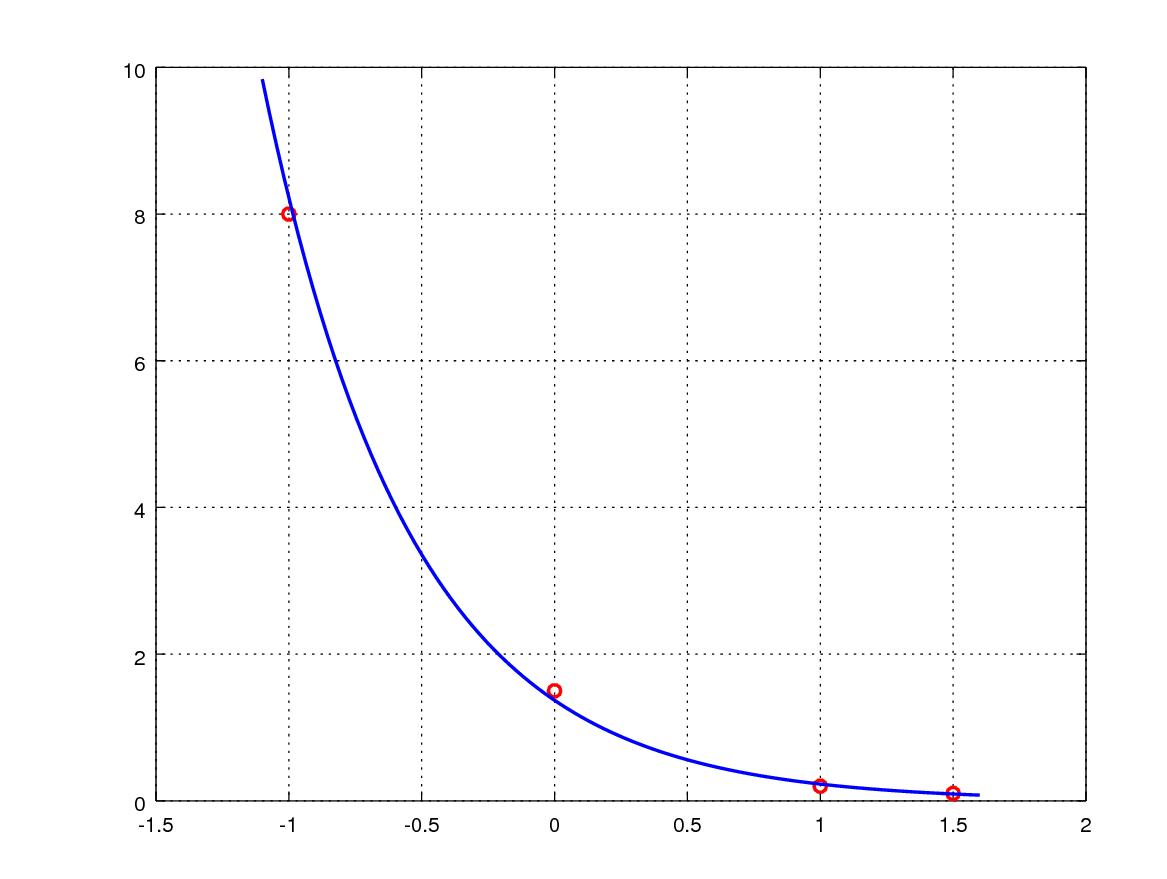
\includegraphics[width=\textwidth]{cap_ajuste/dados/ex_mq_nlin0/ex_mq_nlin0}
  \caption{Esboço da curva ajustada no Exemplo~\ref{ex:mq_nlin0}.}
  \label{fig:ex_mq_nlin0}
\end{figure}

% \ifisoctave
% O ajuste e um esboço da função ajustada podem ser feitos no \verb+GNU Octave+ com o seguinte código:
% \begin{verbatim}
% #pontos
% x = [-1 0 1 1.5]';
% y = [8.0 1.5 0.2 0.1]';

% #resol. as eqs. normais
% A = [ones(4,1) x];
% d = inv(A'*A)*A'*log(y)

% #fun. ajustada
% c = [exp(d(1)); d(2)]
% f = @(x) c(1)*exp(c(2)*x);

% #esboco da fun. ajustada
% xx = linspace(-1.1,1.6);
% plot(x,y,'ro','linewidth',1.5,...
%      xx,f(xx),'b-','linewidth',1.5);grid
% \end{verbatim}
% \fi

\end{ex}

\subsection*{Exercícios}

\begin{flushleft}
  [[tag:revisar]]
\end{flushleft}

\begin{exer}\label{exer:mq_reta}
  Determine a reta $y = c_1x + c_2$ que melhor se ajusta, no sentido de mínimos quadrados, aos pontos
  \begin{center}
    \begin{tabular}{l|ccccc}
      $i$ & $1$ & $2$ & $3$ & $4$ & $5$ \\\hline
      $x_i$ & $-2,5$ & $-1,3$ & $0,2$ & $1,7$ & $2,3$\\
      $y_i$ & $3,8$ & $1,5$ & $-0,7$ & $-1,5$ & $-3,2$\\\hline
    \end{tabular}
  \end{center}
Por fim, compute a norma $L^2$ do resíduo, i.e. $\|r(c)\|_2 = \|y - (c_1x - c_2)\|_2$ para os pontos dados.
\end{exer}
\begin{resp}
  % \ifisoctave 
  % \href{https://github.com/phkonzen/notas/blob/master/src/MatematicaNumerica/cap_ajuste/dados/exer_mq_reta/exer_mq_reta.m}{Código.} 
  % \fi
  $c_1 = -1,3259$, $c_2 = 8,66071\E-2$, $\|r(c)\|_2 = 1,01390$.
\end{resp}

\begin{exer}\label{exer:mq_poli}
  Determine o polinômio $y = c_1x^3 + c_2x^2 + c_3x + c_4$ que melhor se ajusta, no sentido de mínimos quadrados, aos pontos
  \begin{center}
    \begin{tabular}{l|ccccc}
      $i$ & $1$ & $2$ & $3$ & $4$ & $5$ \\\hline
      $x_i$ & $-2,5$ & $-1,3$ & $0,2$ & $1,7$ & $2,3$\\
      $y_i$ & $3,8$ & $0,5$ & $2,7$ & $1,2$ & $-1,3$\\\hline
    \end{tabular}
  \end{center}
Por fim, compute a norma $L^2$ do resíduo, i.e. $\|r(c)\|_2$.
\end{exer}
\begin{resp}
  % \ifisoctave 
  % \href{https://github.com/phkonzen/notas/blob/master/src/MatematicaNumerica/cap_ajuste/dados/exer_mq_poli/exer_mq_poli.m}{Código.} 
  % \fi
  $c_1 = -4,50361\E-1$, $c_2 = -2,78350\E-1$, $c_3 = 1,46291$, $c_4 = 2,09648$, $\|r(c)\|_2 = 5,71346$
\end{resp}

\begin{exer}\label{exer:mq_curva}
  Determine a curva $y = c_1\sen x + c_2\cos x + c_3$ que melhor se ajusta, no sentido de mínimos quadrados, aos pontos
  \begin{center}
    \begin{tabular}{l|ccccc}
      $i$ & $1$ & $2$ & $3$ & $4$ & $5$ \\\hline
      $x_i$ & $-2,5$ & $-1,3$ & $0,2$ & $1,7$ & $2,3$\\
      $y_i$ & $3,8$ & $0,5$ & $2,7$ & $1,2$ & $-1,3$\\\hline
    \end{tabular}
  \end{center}
Por fim, compute a norma $L^2$ do resíduo, i.e. $\|r(c)\|_2$.
\end{exer}
\begin{resp}
  % \ifisoctave 
  % \href{https://github.com/phkonzen/notas/blob/master/src/MatematicaNumerica/cap_ajuste/dados/exer_mq_curva/exer_mq_curva.m}{Código.} 
  % \fi
  $c_1 = -2,76842$, $c_2 = -7,17935\E-1$, $c_3 = 1,37014\E-1$, $\|r(c)\|_2 = 2,48880\E+1$
\end{resp}

\begin{exer}\label{exer:mq_nlin0}
  Use a transformação $z = \ln y$ para ajustar, no sentido de mínimos quadrados, a curva $y = c_1e^{c_2(x-c_3)^2}$ aos pontos
  \begin{center}
    \begin{tabular}{l|cccccc}
      $i$ & $1$ & $2$ & $3$ & $4$ & $5$ & $6$ \\\hline
      $x_i$ & $-0,5$ & $0,5$ & $1,3$ & $2,1$ & $2,7$ & $3,1$ \\
      $y_i$ & $0,1$ & $1,2$ & $2,7$ & $0,9$ & $0,2$ & $0,1$ \\\hline
    \end{tabular}
  \end{center}
\end{exer}
\begin{resp}
  % \ifisoctave 
  % \href{https://github.com/phkonzen/notas/blob/master/src/MatematicaNumerica/cap_ajuste/dados/exer_mq_nlin0/exer_mq_nlin0.m}{Código.} 
  % \fi
  $c_1 = 2,10131\E+0$, $c_2 = -9,73859\E-1$, $c_3 = 1.25521\E+0$
\end{resp}
   
\section{Problemas não lineares}\label{cap_ajuste_sec_prob_nlin}

\begin{flushleft}
  [[tag:revisar]]
\end{flushleft}

Um problema não linear de mínimos quadrados consiste em ajustar uma dada função $f(x;c)$ que dependa não linearmente dos parâmetros $c = (c_1, c_2, \dotsc, c_m)$, $m\geq 1$, a um dado conjunto de $n\geq m$ pontos $\{(x_i, y_i)\}_{i=1}^n$. Mais especificamente, buscamos resolver o seguinte problema de minimização
\begin{equation}\label{eq:prob_nlin_mq}
  \min_{\{c_1, c_2, \dotsc, c_m\}} \left[E := \sum_{i=1}^n \left(y_i - f(x_i;c)\right)^2\right].
\end{equation}
Aqui, denotaremos por $r(c) := (r_1(c), r_2(c), \dotsc, r_n(c))$ o vetor dos resíduos $r_i(c) := y_i - f(x_i,c)$. Com isso, o problema se resume a encontrar o vetor de parâmetros $c$ que minimiza
\begin{equation}
  E = \|r(c)\|_2^2.
\end{equation}
Tais parâmetros são solução do seguinte sistema de equações
\begin{equation}
  \frac{\p E}{\p c_j} = 2\sum_{i=1}^n r_i(c)\frac{\p}{\p c_j}r_i(c) = 0
\end{equation}
ou, equivalentemente, da equação
\begin{equation}\label{eq:grad_E}
  \nabla E = 0 \Leftrightarrow J_R^T(c)r(c) = 0,
\end{equation}
onde
\begin{equation}
  J_R(c) :=
  \begin{bmatrix}
    \frac{\p r_1}{\p c_1} & \frac{\p r_1}{\p c_2} & \cdots & \frac{\p r_1}{\p c_m}\\
    \frac{\p r_2}{\p c_1} & \frac{\p r_2}{\p c_2} & \cdots & \frac{\p r_2}{\p c_m}\\
    \vdots  & \vdots & \vdots & \vdots \\
    \frac{\p r_n}{\p c_1} & \frac{\p r_n}{\p c_2} & \cdots & \frac{\p r_n}{\p c_m}
  \end{bmatrix}
\end{equation}
é a jacobiana do resíduo $r$ em relação aos parâmetros $c$.

Podemos usar o método de Newton para resolver~\eqref{eq:grad_E}. Para tanto, escolhemos uma aproximação inicial para $c^{(1)} = (c_1^{(1)}, c_2^{(1)}, \dotsc, c_m^{(1)})$ e iteramos
\begin{align}
  H_R(c^{(k)})\delta^{(k)} &= -J_R^T(c)r(c) \label{eq:mqnl_newton1}\\
  c^{(k+1)} &= c^{(k)} + \delta^{(k)} \label{eq:mqnl_newton2},
\end{align}
onde $\delta^{(k)} = (\delta_1^{(k)}, \delta_2^{(k)}, \delta_m^{(k)})$ é a atualização de Newton (ou direção de busca) e $H_R(c) := [h_{p,q}(c)]_{p,q=1}^{m,m}$ é a matriz hessiana, cujos elementos são
\begin{equation}
  h_{p,q} := \sum_{i=1}^n\left\{\frac{\p r_i}{\p c_q}\frac{\p r_i}{\p c_p} + r_i\frac{\p^2 r_i}{\p c_q\p c_p}\right\}.
\end{equation}

\begin{ex}\label{ex:mqnl_newton}
  Consideremos o problema de ajustar, no sentido de mínimos quadrados, a função
  \begin{equation}
    f(x;c) = c_1e^{c_2x}
  \end{equation}
ao seguinte conjunto de pontos
\begin{center}
  \begin{tabular}{l|rrrr}
    $i$ & $1$ & $2$ & $3$ & $4$ \\\hline
    $x_i$ & $-1$ & $0$ & $1$ & $1,5$\\
    $y_i$ & $8,0$ & $1,5$ & $0,2$ & $0,1$\\\hline
  \end{tabular}
\end{center}

Aqui, vamos utilizar a iteração de Newton para o problema de mínimos quadrados, i.e. a iteração dada em \eqref{eq:mqnl_newton1}-\eqref{eq:mqnl_newton2}. Para tanto, para cada $i=1, 2, 3, 4$, precisamos das seguintes derivadas parciais do resíduo $r_i(c) := y_i - c_1e^{c_2x_i}$:
\begin{align}
  &\frac{\p}{\p c_1}r_i(c) = - e^{c_2x_i},\\
  &\frac{\p}{\p c_2}r_i(c) = - c_1x_ie^{c_2x_i},\\
  &\frac{\p^2}{\p c_1^2}r_i(c) = 0,\\
  &\frac{\p^2}{\p c_1\p c_2}r_i(c) = \frac{\p^2}{\p c_2\p c_1}r_i(c) = - x_ie^{c_2x_i},\\
  &\frac{\p^2}{\p c_2^2}r_i(c) = - c_1x_i^2e^{c_2x_i}.
\end{align}

\begin{figure}[h]
  \centering
  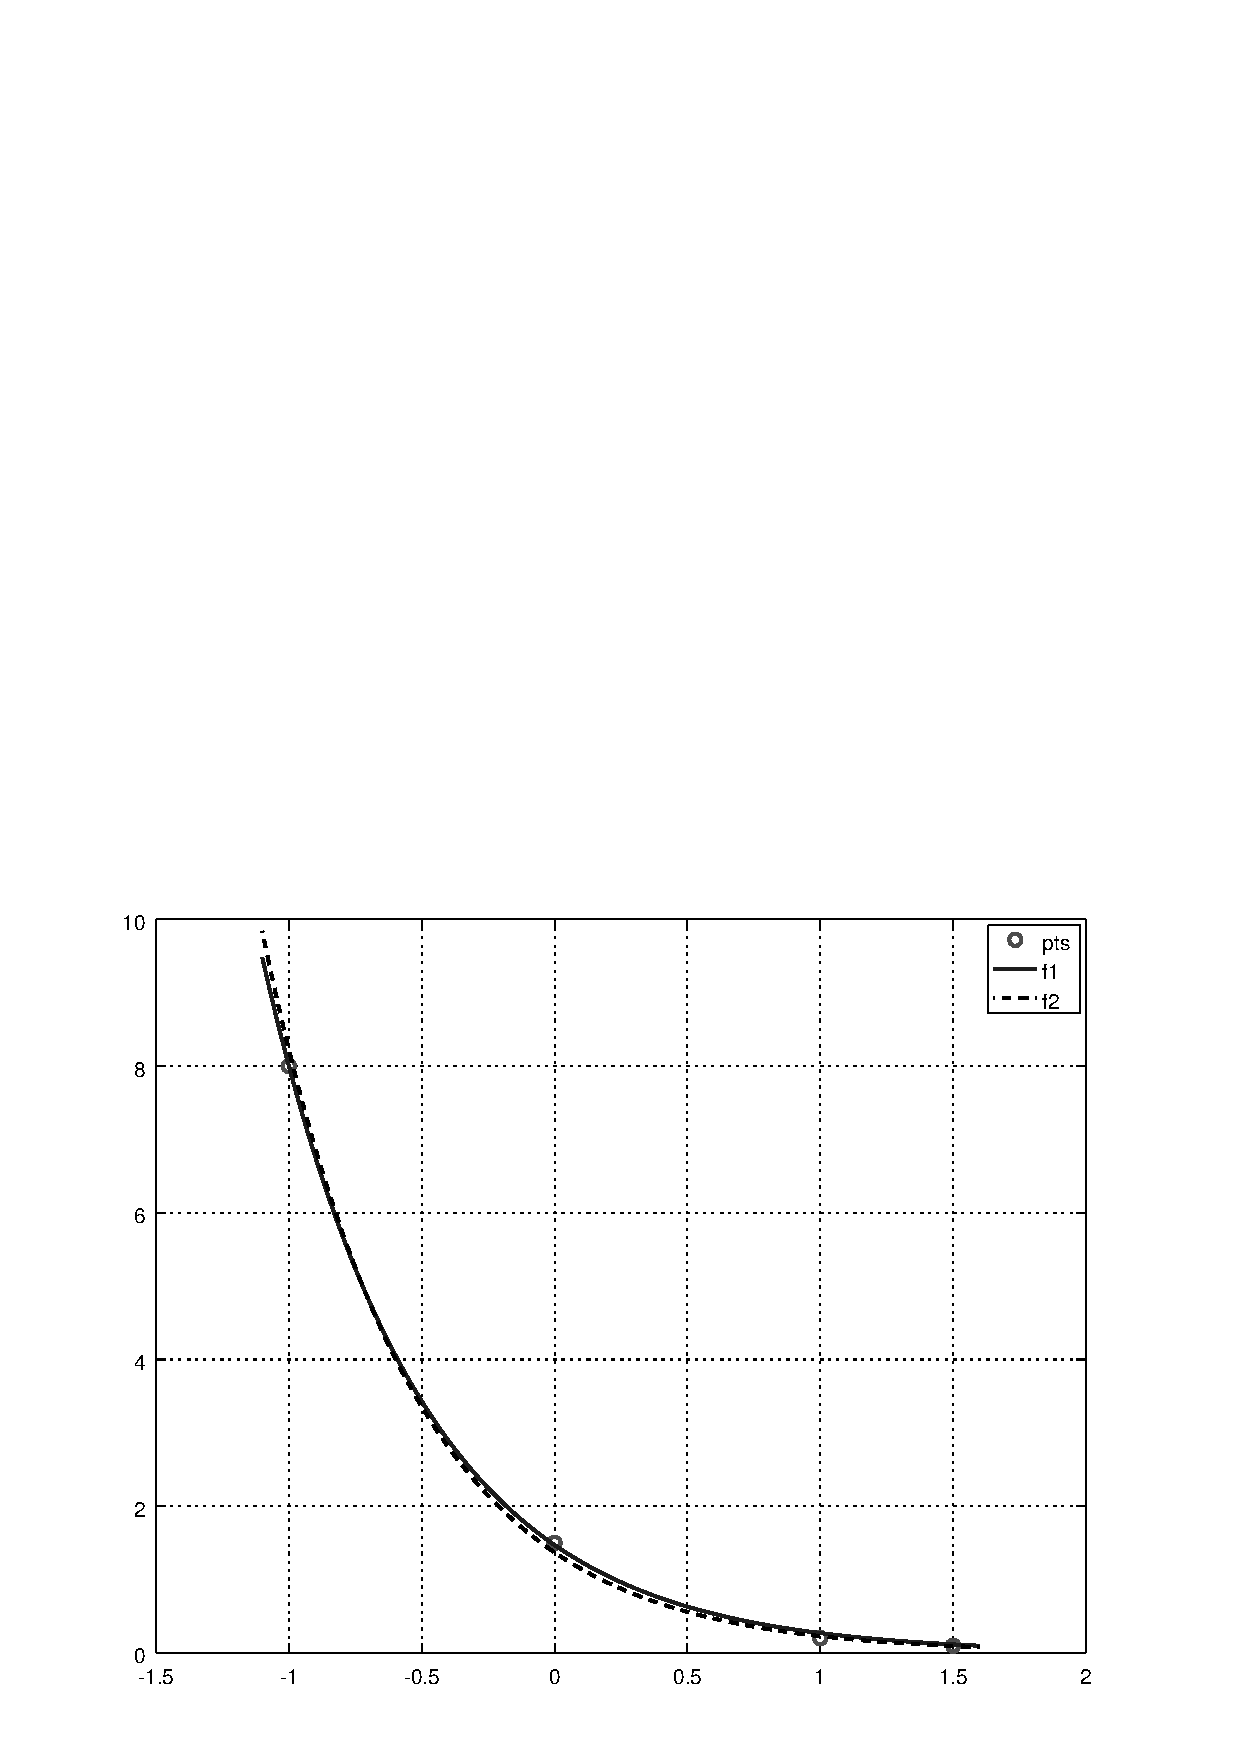
\includegraphics[width=\textwidth]{cap_ajuste/dados/ex_mqnl_N/ex_mqnl_N}
  \caption{Esboço da curva ajustada no Exemplo~\ref{ex:mqnl_newton}.}
  \label{fig:ex_mqnl_newton}
\end{figure}

Com isso e tomando $c^{(1)} = (1,4, ~-1,8)$ (motivado do Exemplo~\ref{ex:mq_nlin0}), computamos as iterações de Newton~\eqref{eq:mqnl_newton1}-\eqref{eq:mqnl_newton2}. Iterando até a precisão de $TOL = 10^{-4}$, obtemos a solução $c_1 = 1,471$ e $c_2 = -1,6938$. Na Figura~\ref{fig:ex_mqnl_newton} vemos uma comparação entre a curva aqui ajustada ($-$) e aquela obtida no Exemplo~\ref{ex:mq_nlin0} ($--$).

% \ifisoctave
% O ajuste discutido neste exemplo pode ser computado no \verb+GNU Octave+ com o seguinte código:
% \begin{verbatim}
% #pontos
% global x = [-1 0 1 1.5]';
% global y = [8.0 1.5 0.2 0.1]';

% #fun. objetivo
% f = @(x,c) c(1)*exp(c(2)*x);

% #residuo
% r = @(c) y - f(x,c);

% #jacobiana
% function A = J(c)
%   global x
%   A = zeros(4,2);
%   A(:,1) = - exp(c(2)*x);
%   A(:,2) = - c(1)*x.*exp(c(2)*x);
% endfunction

% #hessiana
% function A = H(c)
%   global x
%   global y
%   A = zeros(2,2);
%   A = J(c)'*J(c);
%   for i=1:4
%     A(1,1) += 0;
%     A(1,2) += (y(i) - c(1)*exp(c(2)*x(i))) * ...
%               (- x(i)*exp(c(2)*x(i)));
%     A(2,1) += (y(i) - c(1)*exp(c(2)*x(i))) * ...
%               (- x(i)*exp(c(2)*x(i)));
%     A(2,2) += (y(i) - c(1)*exp(c(2)*x(i))) * ...
%               (- c(1)*x(i)^2*exp(c(2)*x(i)));
%   endfor
% endfunction

% #aprox. inicial
% c = [1.4 -1.8]';

% #iteracoes de Newton
% k=0;
% do
%   k+=1;
%   delta = - inv(H(c))*J(c)'*r(c);
%   c = c + delta;
%   [k,c',norm(delta)]
% until ((k>10) | (norm(delta)<1e-4))
% \end{verbatim}
% \fi
\end{ex}

Observamos que a solução obtida no exemplo anterior (Exemplo~\ref{ex:mqnl_newton}) difere da previamente encontrada no Exemplo~\ref{ex:mq_nlin0}. Naquele exemplo, os parâmetros obtidos nos fornecem $E = 6,8\E-2$, enquanto que a solução do exemplo anterior fornece $E = 6,1\E-3$. Isto é esperado, pois naquele exemplo resolvemos um problema aproximado, enquanto no exemplo anterior resolvemos o problema por si.

O emprego do método de Newton para o problema de mínimos quadrados tem a vantagem da taxa de convergência quadrática, entretanto requer a computação das derivadas parciais de segunda ordem do resíduo. Na sequência discutimos alternativas comumente empregadas.

\subsection{Método de Gauss-Newton}

\begin{flushleft}
  [[tag:revisar]]
\end{flushleft}

O método de Gauss-Newton é uma técnica iterativa que aproxima o problema não linear de mínimos quadrados \eqref{eq:prob_nlin_mq} por uma sequência de problemas lineares. Para seu desenvolvimento, começamos de uma aproximação inicial $c^{(1)} = (c_1^{(1)}, c_2^{(1)}, \dotsc, c_m^{(1)})$ dos parâmetros que queremos ajustar. Também, assumindo que a $n$-ésima iterada $c^{(k)}$ é conhecida, faremos uso da aproximação de primeira ordem de $f(x,c)$ por polinômio de Taylor, i.e.
\begin{equation}
  f(x;c^{(k+1)}) \approx f(x;c^{(k)}) + \nabla_c f(x;c^{(k)})(c^{(k+1)}-c^{(k)}),
\end{equation}
onde
\begin{equation}
  \nabla_c f(x;c) = \left[\frac{\p}{\p c_1}f(x;c) ~\frac{\p}{\p c_2}f(x;c) ~\cdots ~\frac{\p}{\p c_m}f(x;c)\right].
\end{equation}

O método consiste em obter a solução do problema não linear \eqref{eq:prob_nlin_mq} pelo limite dos seguintes problemas lineares de mínimos quadrados
\begin{align}
  \min_{\delta^{(k)}} &\left[\tilde{E} := \sum_{i=1}^n (y_i - f(x_i,c^{(k)}) - \nabla_c f(x_i;c^{(k)})\delta^{(k)})^2\right] \label{eq:mq_gn0}\\
  &c^{(k+1)} = c^{(k)} + \delta^{(k)}.
\end{align}

Agora, usando a notação de resíduo $r(c) = y - f(x;c)$, observamos que \eqref{eq:mq_gn0} consiste no problema linear de mínimos quadrados
\begin{equation}
  \min_{\delta^{(k)}} \|r(c^{(k)}) + J_R(c^{(k)})\delta^{(k)}\|_2^2,
\end{equation}
o qual é equivalente a resolver as equações normais
\begin{equation}
  J_R^T(c^{(n)})J_R(c^{(n)})\delta^{(n)} = -J_R^T(c)r(c).
\end{equation}

Com isso, dada uma aproximação inicial $c^{(1)}$, a \emph{iteração do método de Gauss-Newton} consiste em
\begin{align}
  &J_R^T(c^{(k)})J_R(c^{(k)})\delta^{(k)} = -J_R^T(c)r(c)\\
  &c^{(k+1)} = c^{(k)} + \delta^{(k)}.
\end{align}

\begin{ex}
  A aplicação da iteração de Gauss-Newton ao problema de mínimos quadrados discutido no Exemplo~\ref{ex:mqnl_newton} nos fornece a mesma solução obtida naquele exemplo (preservadas a aproximação inicial e a tolerância de precisão).

% \ifisoctave
% A implementação do método de Gauss-Newton para este problema no \verb+GNU Octave+ pode ser feita com o seguinte código:
% \begin{verbatim}
% #pontos
% global x = [-1 0 1 1.5]';
% y = [8.0 1.5 0.2 0.1]';

% #fun. objetivo
% f = @(x,c) c(1)*exp(c(2)*x);

% #residuo
% r = @(c) y - f(x,c);

% #jacobiana
% function A = J(c)
%   global x
%   A = zeros(4,2);
%   A(:,1) = - exp(c(2)*x);
%   A(:,2) = - c(1)*x.*exp(c(2)*x);
% endfunction

% #aprox. inicial
% c = [1.4 -1.8]';

% #iteracoes de Gauss-Newton
% k=0;
% do
%   k+=1;
%   delta = - inv(J(c)'*J(c))*J(c)'*r(c);
%   c = c + delta;
%   [k,c',norm(delta)]
% until ((k>10) | (norm(delta)<1e-4))
% \end{verbatim}
% \fi
\end{ex}

O método de Gauss-Newton pode ser lentamente convergente para problemas muito não lineares ou com resíduos grandes. Nesse caso, métodos de Gauss-Newton com amortecimento são alternativas robustas~\cite{Bjorck1996a,Nocedal2006a}. Na sequência, introduziremos um destes métodos, conhecido como método de Levenberg-Marquardt.

\subsection{Método de Levenberg-Marquardt}

\begin{flushleft}
  [[tag:revisar]]
\end{flushleft}

O método de Levenberg-Marquardt é uma variação do método de Gauss-Newton no qual a direção de busca $\delta^{(n)}$ é obtida da solução do seguinte problema regularizado
\begin{equation} \label{eq:mq_gn0}
  \min_{\delta^{(k)}} \{\|r(c^{(k)}) + J_R(c^{(k)})\delta^{(k)}\|_2^2 + \mu^{(k)}\|\delta^{(k)}\|_2^2\}
\end{equation}
ou, equivalentemente,
\begin{equation} \label{eq:mq_gn0}
  \min_{\delta^{(k)}} \left\|
    \begin{bmatrix}
      r(c^{(k)})\\
      0
    \end{bmatrix} +
    \begin{bmatrix}
      J_R(c^{(k)})\\
      \mu^{(k)}I
    \end{bmatrix}
    \delta^{(k)}\right\|_2^2
\end{equation}

A taxa de convergência das iterações de Levenberg-Marquardt é sensível a escolha do parâmetro $\mu^{(k)}\geq 0$. Aqui, faremos esta escolha por tentativa e erro. O leitor pode aprofundar-se mais sobre esta questão na literatura especializada (veja, por exemplo, \cite{Bjorck1996a,Nocedal2006a}).

\begin{obs}
  Quando $\mu^{(k)} \equiv 0$ para todo $n$, o método de Levenberg-Marquardt é equivalente ao método de Gauss-Newton.
\end{obs}

\begin{ex}\label{ex:mqnl_LM}
  Consideremos o problema de mínimos quadrados discutido no Exemplo~\ref{ex:mqnl_newton}. O método de Gauss-Newton falha para este problema se escolhermos, por exemplo, $c^{(1)} = (0, 0)$. Isto ocorre pois, para esta escolha de $c^{(1)}$, a jacobiana $J(c^{(1)})$ não tem posto completo. Entretanto, o método de Levenberg-Marquardt com $\mu^{(k)} = 0,1$ é convergente, mesmo para esta escolha de $c^{(1)}$.

% \ifisoctave
% A implementação no \verb+GNU Octave+ do método de Levenberg-Marquardt (com $\mu^{(k)}=0,1$ constante) para este problema pode ser feita com o seguinte código:
% \begin{verbatim}
% #pontos
% global x = [-1 0 1 1.5]';
% y = [8.0 1.5 0.2 0.1]';

% #fun. objetivo
% f = @(x,c) c(1)*exp(c(2)*x);

% #residuo
% r = @(c) y - f(x,c);

% #jacobiana
% function A = JR(c)
%   global x;
%   A = zeros(4,2);
%   A(:,1) = - exp(c(2)*x);
%   A(:,2) = - c(1)*x.*exp(c(2)*x);
% endfunction

% #aprox. inicial
% c = [0 0]';

% #param. de amortecimento
% mu = 0.1;

% #iteracoes de Gauss-Newton
% k=0;
% do
%   k+=1;
%   JJ = [JR(c);mu*eye(2,2)];
%   delta = - inv(JJ'*JJ)*JJ'*[r(c);zeros(2,1)];
%   c = c + delta;
%   printf("%d %1.1e %1.3e %1.3e\n", k,norm(delta),c')
% until ((k>10) | (norm(delta)<1e-4))
% \end{verbatim}
% \fi
\end{ex}

\subsection*{Exercícios}

\begin{flushleft}
  [[tag:revisar]]
\end{flushleft}

\begin{exer}\label{exer:mqnl_GN}
  Use o método de Gauss-Newton para ajustar, no sentido de mínimos quadrados e com precisão de $10^{-4}$, a curva $y = c_1e^{c_2(x-c_3)^2}$ aos pontos
  \begin{center}
    \begin{tabular}{l|cccccc}
      $i$ & $1$ & $2$ & $3$ & $4$ & $5$ & $6$ \\\hline
      $x_i$ & $-0,5$ & $0,5$ & $1,3$ & $2,1$ & $2,7$ & $3,1$ \\
      $y_i$ & $0,1$ & $1,2$ & $2,7$ & $0,9$ & $0,2$ & $0,1$ \\\hline
    \end{tabular}
  \end{center}
Use as condições iniciais:
\begin{enumerate}[a)]
\item $c_1 = 2,1$, $c_2=-1$ e $c_3=1,3$.
\item $c_1=1$, $c_2=-1$ e $c_3=-1$.
\end{enumerate}
\end{exer}
\begin{resp}
  % \ifisoctave 
  % \href{https://github.com/phkonzen/notas/blob/master/src/MatematicaNumerica/cap_ajuste/dados/exer_mqnl_GN/exer_mqnl_GN.m}{Código.} 
  % \fi
  a) $c_1 = 2,69971\E+0$, $c_2 = -1,44723\E+0$, $c_3 = 1.24333\E+0$; b) divergente.
\end{resp}

\begin{exer}
  Resolva o exercício anterior (Exercício~\ref{exer:mqnl_GN}) usando o método de Levenberg-Marquardt com amortecimento constante $\mu=0,2$.
\end{exer}
\begin{resp}
  % \ifisoctave 
  % \href{https://github.com/phkonzen/notas/blob/master/src/MatematicaNumerica/cap_ajuste/dados/exer_mqnl_LM/exer_mqnl_LM.m}{Código.} 
  % \fi
  a)  $c_1 = 2,69971\E+0$, $c_2 = -1,44723\E+0$, $c_3 = 1.24333\E+0$; b) $c_1 = 2,69971\E+0$, $c_2 = -1,44723\E+0$, $c_3 = 1.24333\E+0$
\end{resp}

%Este trabalho está licenciado sob a Licença Atribuição-CompartilhaIgual 4.0 Internacional Creative Commons. Para visualizar uma cópia desta licença, visite http://creativecommons.org/licenses/by-sa/4.0/deed.pt_BR ou mande uma carta para Creative Commons, PO Box 1866, Mountain View, CA 94042, USA.

\chapter{Derivação}\label{cap_deriv}
\thispagestyle{fancy}

Neste capítulo, discutimos os métodos fundamentais de derivação numérica de funções.

\section{Derivadas de primeira ordem}\label{cap_deriv_sec_df}

A derivada de uma função $f$ num ponto $x$ é, por definição,
\begin{equation}
  f'(x) = \lim_{h\to 0} \frac{f(x+h) - f(x)}{h}.
\end{equation}
Assim sendo e assumindo $h>0$\footnote{Para fixar notação, assumiremos $h>0$ ao longo deste capítulo.} próximo de zero, temos que $f'(x)$ pode ser aproximada pela razão fundamental, i.e.
\begin{equation}\label{eq_razao_fundamental}
  f'(x) \approx \underbrace{\frac{f(x+h) - f(x)}{h}}_{D_hf(x)}.
\end{equation}
Analisando a Figura~\ref{fig:intro_deriv} vemos que, geometricamente, isto é análogo a aproximar a declividade da reta tangente ao gráfico da função $f$ no ponto $(x,f(x))$ pela declividade da reta secante ao gráfico da função $f$ pelos pontos $(x,f(x))$ e $(x+h,f(x+h))$.

\begin{figure}[hp]
  \centering
  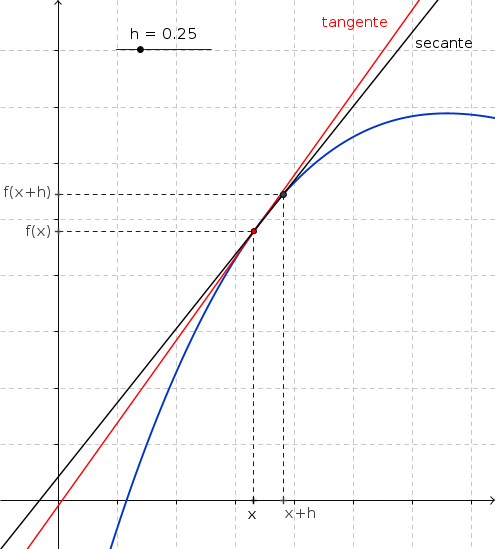
\includegraphics[width=0.7\textwidth]{cap_deriv/dados/fig_intro_deriv/fig_intro_deriv}
  \caption{Interpretação geométrica da aproximação da derivada pela razão fundamental. Veja no \href{https://github.com/phkonzen/notas/blob/master/src/MatematicaNumerica/cap_deriv/dados/fig_intro_deriv/fig_intro_deriv.ggb}{Geogebra}.}
  \label{fig:intro_deriv}
\end{figure}

\begin{ex}\label{ex_intro_deriv}
  A derivada de $f(x) = \sen(x)$ no ponto $\pi/3$ é $f'(\pi/3) = \cos(\pi/3)=0,5$. Agora, usando a aproximação pela razão fundamental~\eqref{eq_razao_fundamental}, temos
  \begin{align}
    f'\left(\frac{\pi}{3}\right) \approx D_hf(x) &= \frac{f\left(\frac{\pi}{3}+h\right)-f\left(\frac{\pi}{3}\right)}{h}\\
          &= \frac{\sen\left(\frac{\pi}{3}\right)-\sen\left(\frac{\pi}{3}\right)}{h}. 
  \end{align}
Na Tabela~\ref{tab:ex_intro_deriv} temos os valores desta aproximação para diferentes escolhas da passo $h$.

\begin{table}[hp]
  \centering
  \begin{tabular}{l|c}
    $h$ & $Df(\pi/3)$ \\ \hline
    $10^{-1}$ & $4,55902\E-1$ \\
    $10^{-2}$ & $4,95662\E-1$ \\
    $10^{-3}$ & $4,99567\E-1$ \\
    $10^{-5}$ & $4,99996\E-1$ \\
    $10^{-10}$ & $5.00000\E-1$ \\\hline
  \end{tabular}
  \caption{Valores aproximados da derivada de $f(x)=\sen(x)$ no ponto $x=\pi/6$ usado a expressão~\eqref{eq_razao_fundamental}.}
  \label{tab:ex_intro_deriv}
\end{table}

No \verb+GNU Octave+, podemos fazer estes cálculos com o seguinte código:
\begin{verbatim}
f = @(x) sin(x);
Df = @(x,h) (f(x+h)-f(x))/h;
x=pi/3;
h=1e-1;
printf('%1.5e\n',Df(x,h))
\end{verbatim}
\end{ex}

A aproximação~\eqref{eq_razao_fundamental} é uma \emph{fórmula de diferenças finitas}\index{fórmula de diferenças finitas}. Existem várias aproximações deste tipo que podem ser derivadas. Além disso, tais derivações nos permitem estimar o erro na utilização de tais fórmulas para a aproximação de derivadas. Na sequência, discutiremos o desenvolvimento de fórmulas de diferenças finitas usando polinômios de Taylor.

\subsection{Desenvolvimento por polinômio de Taylor}

Aqui, discutimos a obtenção de fórmulas de diferenças finitas via polinômio de Taylor.

\subsubsection{Diferenças finitas progressiva de ordem $h$}

A aproximação por polinômio de Taylor de grau 1 de uma dada função $f$ em torno no ponto $x$ é
\begin{equation}\label{eq:poli_Taylor_grau_1}
  f(x+h) = f(x) + hf'(x) + O(h^2).
\end{equation}
Agora, isolando $f'(x)$, obtemos
\begin{equation}
  f'(x) = \frac{f(x+h) - f(x)}{h} + O(h).
\end{equation}
Isto nos fornece a chamada fórmula de diferenças finitas progressiva de ordem $h$\index{fórmula de diferenças finitas!progressiva de ordem $h$}
\begin{equation}\label{eq:dfp_h}
  D_{+,h}f(x) := \frac{f(x+h) - f(x)}{h}.
\end{equation}
Observemos que a ordem da fórmula se refere a ordem do \emph{erro de truncamento}\index{erro de!truncamento} com respeito ao passo $h$.

\begin{ex}\label{ex:dfp_h}
  Consideremos o problema de aproximar a derivada da função $f(x) = \sen(x)$ no ponto $\pi/3$. Usando a fórmula de diferenças finitas progressiva de ordem $h$ obtemos
  \begin{align}
    f'\left(\frac{\pi}{3}\right) \approx D_{+,h}f(x) &= \frac{f\left(\frac{\pi}{3}+h\right)-f\left(\frac{\pi}{3}\right)}{h}\\
          &= \frac{\sen\left(\frac{\pi}{3}+h\right)-\sen\left(\frac{\pi}{3}\right)}{h}. 
  \end{align}
Na Tabela~\ref{tab:ex_dfp_h} temos os valores desta aproximação para diferentes escolhas de $h$, bem como, o erro absoluto da aproximação de $f'(\pi/3)$ por $D_{+,h}f(\pi/3)$.

\begin{table}[h!]
  \centering
  \caption{Resultados referente ao Exemplo~\ref{ex:dfp_h}.}
  \begin{tabular}{l|c|c}
    $h$ & $D_{+,h}f(\pi/3)$ & $|f'(\pi/3)-D_{+,h}f(\pi/3)|$\\ \hline
    $10^{-1}$ & $4,55902\E-1$ & $4,4\E-2$ \\
    $10^{-2}$ & $4,95662\E-1$ & $4,3\E-3$ \\
    $10^{-3}$ & $4,99567\E-1$ & $4,3\E-4$ \\
    $10^{-5}$ & $4,99996\E-1$ & $4,3\E-6$ \\
    $10^{-10}$ & $5.00000\E-1$ & $4,1\E-8$ \\\hline
  \end{tabular}
  \label{tab:ex_dfp_h}
\end{table}

No \verb+GNU Octave+, podemos fazer estes cálculos com o seguinte código:
\begin{verbatim}
f = @(x) sin(x);
Df = @(x,h) (f(x+h)-f(x))/h;
x=pi/3;
h=1e-1;
printf('%1.5e %1.1e\n',Df(x,h),abs(cos(x)-Df(x,h)))
\end{verbatim}
\end{ex}

\begin{obs}
  No exemplo acima (Exemplo~\ref{ex:dfp_h}), podemos observar que o erro absoluto na aproximação de $f'(x)$ por $D_{+,h}f(x)$ decresce conforme a ordem do erro de truncamento para valores moderados de $h$ (veja, Tabela~\ref{tab:ex_dfp_h}). Agora, para valores de $h$ muito pequenos (por exemplo, $h=10^{-10}$), o erro $|f'(x)-D_{+,h}f(x)|$ não segue mais a tendência de decaimento na mesma do de truncamento. Isto se deve a dominância dos erros de arredondamento para valores muito pequenos de $h$. 

  Para mais informações sobre o comportamento do erro de arredondamento em fórmulas de diferenças finitas, veja, por exemplo, \href{https://www.ufrgs.br/reamat/CalculoNumerico/livro-oct/dn-diferencas_finitas.html}{REAMAT - Cálculo Numérico - Versão GNU Octave - Diferenças Finitas - Erro de arredondamento}.
\end{obs}

\subsubsection{Diferenças finitas regressiva de ordem $h$}

Substituindo $h$ por $-h$ na equação~\eqref{eq:poli_Taylor_grau_1}, obtemos
\begin{equation}
  f(x-h) = f(x) - hf'(x) + O(h^2),
\end{equation}
donde obtemos a fórmula de diferenças finitas regressiva de ordem $h$\index{fórmula de diferenças finitas!regressiva de ordem $h$}
\begin{equation}\label{eq:dfr_h}
  D_{-,h}f(x) = \frac{f(x) - f(x-h)}{h}.
\end{equation}

\begin{ex}\label{ex:dfr_h}
  Consideremos o problema de aproximar a derivada da função $f(x) = \sen(x)$ no ponto $\pi/3$. Usando a fórmula de diferenças finitas regressiva de ordem $h$ obtemos
  \begin{align}
    f'\left(\frac{\pi}{3}\right) \approx D_{-,h}f(x) &= \frac{f\left(\frac{\pi}{3}\right)-f\left(\frac{\pi}{3}-h\right)}{h}\\
          &= \frac{\sen\left(\frac{\pi}{3}\right)-\sen\left(\frac{\pi}{3}-h\right)}{h}. 
  \end{align}
Na Tabela~\ref{tab:ex_dfr_h} temos os valores desta aproximação para diferentes escolhas de $h$, bem como, o erro absoluto da aproximação de $f'(\pi/3)$ por $D_{-,h}f(\pi/3)$.

\begin{table}[h!]
  \centering
  \caption{Resultados referente ao Exemplo~\ref{ex:dfr_h}.}
  \begin{tabular}{l|c|c}
    $h$ & $D_{-,h}f(\pi/3)$ & $|f'(\pi/3)-D_{-,h}f(\pi/3)|$\\ \hline
    $10^{-1}$ & $5,42432\E-1$ & $4,2\E-2$ \\
    $10^{-2}$ & $5,04322\E-1$ & $4,3\E-3$ \\
    $10^{-3}$ & $5,00433\E-1$ & $4,3\E-4$ \\
    $10^{-5}$ & $5,00004\E-1$ & $4,3\E-6$ \\
    $10^{-10}$ & $5.00000\E-1$ & $4,1\E-8$ \\\hline
  \end{tabular}
  \label{tab:ex_dfr_h}
\end{table}

No \verb+GNU Octave+, podemos fazer estes cálculos com o seguinte código:
\begin{verbatim}
f = @(x) sin(x);
Df = @(x,h) (f(x)-f(x-h))/h;
x=pi/3;
h=1e-1;
printf('%1.5E %1.1E\n',Df(x,h),abs(cos(x)-Df(x,h)))
\end{verbatim}
\end{ex}

\subsubsection{Diferenças finitas central de ordem $h^2$}

Usando o polinômio de Taylor de grau 2 para aproximar a função $f(x)$ em torno de $x$, obtemos
\begin{align}
  f(x+h) &= f(x) + hf'(x) + \frac{h}{2}f''(x) + O(h^3)\\
  f(x-h) &= f(x) - hf'(x) + \frac{h}{2}f''(x) + O(h^3).
\end{align}
Então, subtraindo esta segunda equação da primeira, temos
\begin{equation}
  f(x+h)-f(x-h) = 2hf'(x) + O(h^3).
\end{equation}
Agora, isolando $f(x)$
\begin{equation}
  f'(x) = \frac{f(x+h)-f(x-h)}{2h} + O(h^2),
\end{equation}
o que nos fornece a chamada fórmula de diferenças finitas central de ordem $h^2$\index{fórmula de diferenças finitas!central de ordem $h^2$}
\begin{equation}\label{eq:dfc_h2}
  D_{0,h^2}f(x) := \frac{f(x+h)-f(x-h)}{2h}.
\end{equation}

\begin{ex}\label{ex:dfc_h2}
  Consideremos o problema de aproximar a derivada da função $f(x) = \sen(x)$ no ponto $\pi/3$. Usando a fórmula de diferenças finitas central de ordem $h^2$ obtemos
  \begin{align}
    f'\left(\frac{\pi}{3}\right) \approx D_{0,h^2}f(x) &= \frac{f\left(\frac{\pi}{3}+h\right)-f\left(\frac{\pi}{3}-h\right)}{2h}\\
          &= \frac{\sen\left(\frac{\pi}{3}+h\right)-\sen\left(\frac{\pi}{3}-h\right)}{2h}. 
  \end{align}

\begin{table}[h!]
  \centering
  \caption{Resultados referente ao Exemplo~\ref{ex:dfc_h2}.}
  \begin{tabular}{l|c|c}
    $h$ & $D_{0,h^2}f(\pi/3)$ & $|f'(\pi/3)-D_{0,h^2}f(\pi/3)|$\\ \hline
    $10^{-1}$ & $4,99167\E-1$ & $8,3\E-04$ \\
    $10^{-2}$ & $4,99992\E-1$ & $8,3\E-06$ \\
    $10^{-3}$ & $5,00000\E-1$ & $8,3\E-08$ \\
    $10^{-5}$ & $5,00000\E-1$ & $8,3\E-10$ \\
    $10^{-10}$ & $5.00000\E-1$ & $7,8\E-12$ \\\hline
  \end{tabular}
  \label{tab:ex_dfc_h2}
\end{table}

Na Tabela~\ref{tab:ex_dfc_h2} temos os valores desta aproximação para diferentes escolhas de $h$, bem como, o erro absoluto da aproximação de $f'(\pi/3)$ por $D_{0,h^2}f(\pi/3)$.

No \verb+GNU Octave+, podemos fazer estes cálculos com o seguinte código:
\begin{verbatim}
f = @(x) sin(x);
Df = @(x,h) (f(x+h)-f(x-h))/(2*h);
x=pi/3;
h=1e-1;
printf('%1.5E %1.1E\n',Df(x,h),abs(cos(x)-Df(x,h)))
\end{verbatim}
\end{ex}


\subsection*{Exercícios}

\begin{exer}\label{exer:df_fun}
  Calcule aproximações da derivada de
  \begin{equation}
    f(x) = \frac{\sen(x+2) - e^{-x^2}}{x^2 + \ln(x+2)}+x
  \end{equation}
no ponto $x=2,5$ dadas pelas seguintes fórmulas de diferenças finitas com $h=10^{-2}$:
\begin{enumerate}[a)]
\item progressiva de ordem $h$.
\item regressiva de ordem $h$.
\item central de ordem $h^2$.
\end{enumerate}
\end{exer}
\begin{resp}
  % \ifisoctave 
  % \href{https://github.com/phkonzen/notas/blob/master/src/MatematicaNumerica/cap_deriv/dados/exer_df_fun/exer_df_fun.m}{Código.} 
  % \fi
  a)~$D_{+,h}f(2,5)=1,05949$; b)~$D_{-,h}f(2,5)=1,05877$; c)~$D_{0,h^2}f(2,5)=1,05913$;
\end{resp}

\begin{exer}\label{exer:df_tab}
  Considere a seguinte tabela de pontos
  \begin{center}
    \begin{tabular}{l|cccccc}
      $i$ & $1$ & $2$ & $3$ & $4$ & $5$ & $6$ \\\hline
      $x_i$ & $2,0$ & $2,1$ & $2,2$ & $2,3$ & $2,4$ & $2,5$ \\
      $y_i$ & $1,86$ & $1,90$ & $2,01$ & $2,16$ & $2,23$ & $2,31$ \\\hline
    \end{tabular}
  \end{center}
Calcule aproximações de $dy/dx$ usando diferenças finitas centrais de ordem $h^2$ quando possível e, caso contrário, diferenças finitas progressiva ou regressiva conforme o caso.
\end{exer}
\begin{resp}
  % \ifisoctave 
  % \href{https://github.com/phkonzen/notas/blob/master/src/MatematicaNumerica/cap_deriv/dados/exer_df_tab/exer_df_tab.m}{Código.} 
  % \fi
  \begin{center}
    \begin{tabular}{l|cccccc}\hline
      $i$ & $1$ & $2$ & $3$ & $4$ & $5$ & $6$ \\
      $dy/dx$ & $4,0\E-1$ & $7,5\E-1$ & $1,3\E+0$ & $1,1\E+0$ & $7,5\E-1$ & $8,0\E-1$ \\\hline
    \end{tabular}
  \end{center}
\end{resp}

\section{Derivadas de segunda ordem}\label{cap_deriv_sec_d2f}\index{fórmula de diferenças finitas!derivada segunda}

Diferentemente do que é costumeiro em técnicas analíticas, no âmbito da matemática numérica é preferível obter aproximações diretas de derivadas de segunda ordem, em vez de utilizar aproximações sucessivas de derivadas de primeira ordem. Na sequência, desenvolveremos e aplicaremos uma fórmula de diferenças finitas central para a aproximação de derivadas de segunda ordem.

Consideremos os seguintes polinômios de Taylor de grau 3 de $f(x)$ em torno do ponto x
\begin{align}
  f(x+h) &= f(x) + hf'(x) + \frac{h^2}{2}f''(x) + \frac{h^3}{3!}f'''(x) + O(h^4),\\
  f(x-h) &= f(x) - hf'(x) + \frac{h^2}{2}f''(x) - \frac{h^3}{3!}f'''(x) + O(h^4).\\
\end{align}
Somando estas duas equações, obtemos
\begin{equation}
  f(x+h)+f(x-h) = 2f(x) + h^2f''(x) + O(h^4).
\end{equation}
Então, isolando $f''(x)$ temos
\begin{equation}
  f''(x) = \frac{f(x+h) - 2f(x) + f(x-h)}{h^2} + O(h^2).
\end{equation}
Isto nos leva a definição da \emph{fórmula de diferenças finitas de ordem $h^2$ para a derivada segunda}
\begin{equation}
  D_{0,h^2}^2 f(x) := \frac{f(x+h) - 2f(x) + f(x-h)}{h^2}.
\end{equation}

\begin{ex}\label{ex:d2fc_h2}
  Consideremos o problema de computar a derivada segunda de $f(x) = x^2 + \sen x$ no ponto $x=\pi/6$. Analiticamente, $f''(\pi/6) = 2 - \sen(\pi/6) = 1,5$. Numericamente, vamos explorar as seguintes duas aproximações:
  \begin{enumerate}
  \item[a)] Aplicação de sucessivas diferenças finitas centrais de ordem $h^2$ para derivada primeira, i.e.
    \begin{equation}\label{eq:ddf}
      f''(x) \approx D_{0,h^2}D_{0,h^2}f(x) = \frac{D_{0,h^2}f(x+h) - D_{0,h^2}f(x-h)}{2h}
    \end{equation}
  \item[b)] Aplicação da fórmula de diferenças finitas central de ordem $h^2$ para a derivada segunda, i.e.
    \begin{equation}
      f''(x) \approx D_{0,h^2}^2 f(x) = \frac{f(x+h) - 2f(x) + f(x-h)}{h^2}.
    \end{equation}
  \end{enumerate}

\begin{table}[h!]
  \centering
  \caption{Resultados referente ao Exemplo~\ref{ex:d2fc_h2}. Notação: $\delta_{DD}:=|f''(\pi/6)-D_{0,h^2}D_{0,h^2}f(\pi/6)|$ e $\delta_{D^2}:=|f''(\pi/6)-D^2_{0,h^2}f(\pi/6)|$.}
  \begin{tabular}{l|cc|cc}
    $h$ & $D_{0,h^2}D_{0,h^2}f(\pi/6)$ & $\delta_{DD}$ & $D^2_{0,h^2}f(\pi/6)$ & $\delta_{D^2}$ \\ \hline
    $10^{-1}$ &  $1,50166$ & $1,7\E-03$ & $1,50042$ & $4,2\E-04$ \\
    $10^{-2}$ &  $1,50002$ & $1,7\E-05$ & $1,50000$ & $4,2\E-06$ \\
    $10^{-3}$ &  $1,50000$ & $1,7\E-07$ & $1,50000$ & $4,2\E-08$ \\
    $10^{-5}$ &  $1,50000$ & $1,2\E-07$ & $1,50000$ & $1,2\E-07$ \\\hline
  \end{tabular}
  \label{tab:ex_d2fc_h2}
\end{table}

Na Tabela~\ref{tab:ex_d2fc_h2} temos os valores computados em ambos os casos e seus respectivos erros absolutos para diversas escolhas de $h$. Observamos que a aplicação da diferença finita $D^2_{0,h^2}$ fornece resultados mais precisos (para valores moderados de $h$) do que as sucessivas aplicações de $D_{0,h^2}$. De fato, uma rápida inspeção de \eqref{eq:ddf} mostra que
\begin{equation}
  D_{0,h^2}D_{0,h^2}f(x) = \underbrace{\frac{f(x+2h) - 2f(x) + f(x-2h)}{4h^2}}_{D^2_{0,(2h)^2}f(x)}.
\end{equation}

No \verb+GNU Octave+, podemos fazer estes cálculos com o seguinte código:
\begin{verbatim}
f = @(x) sin(x) + x^2;
Df = @(x,h) (f(x+h)-f(x-h))/(2*h);
DDf = @(x,h) (Df(x+h,h)-Df(x-h,h))/(2*h);
D2f = @(x,h) (f(x+h) - 2*f(x) + f(x-h))/(h^2);
x=pi/6;
h=1e-1;
printf('%1.5E %1.1E %1.5E %1.1E\n',...
  DDf(x,h),abs(1.5-DDf(x,h)),...
  D2f(x,h),abs(1.5-D2f(x,h)))
\end{verbatim}
\end{ex}

\subsection*{Exercícios}

\begin{exer}\label{exer:d2fc_fun}
  Use a fórmula de diferenças finitas central de ordem $h^2$ para computar aproximações da segunda derivada de
  \begin{equation}
    f(x) = \frac{\sen(x+2) - e^{-x^2}}{x^2 + \ln(x+2)}+x
  \end{equation}
no ponto $x=2,5$. Para tanto, use os passos
\begin{enumerate}[a)]
\item $h=10^{-1}$
\item $h=10^{-2}$
\item $h=10^{-3}$
\item $h=10^{-4}$
\end{enumerate}
Por fim, com base nos resultados obtidos, qual foi o maior passo que forneceu a aproximação com precisão de pelo menos $5$ dígitos significativos? Justifique sua resposta.
\end{exer}
\begin{resp}
  % \ifisoctave 
  % \href{https://github.com/phkonzen/notas/blob/master/src/MatematicaNumerica/cap_deriv/dados/exer_d2fc_fun/exer_d2fc_fun.m}{Código.} 
  % \fi
  a)~$7,25162\E-2$; b)~$7.24701\E-2$; c)~$7,24696\E-2$; d)~$7,24696\E-2$; $h=10^{-2}$;
\end{resp}

\begin{exer}\label{exer:d2fc_tab}
  Considere a seguinte tabela de pontos
  \begin{center}
    \begin{tabular}{l|cccccc}
      $i$ & $1$ & $2$ & $3$ & $4$ & $5$ & $6$ \\\hline
      $x_i$ & $2,0$ & $2,1$ & $2,2$ & $2,3$ & $2,4$ & $2,5$ \\
      $y_i$ & $1,86$ & $1,90$ & $2,01$ & $2,16$ & $2,23$ & $2,31$ \\\hline
    \end{tabular}
  \end{center}
Calcule a aproximação $d^2y/dx^2$ no ponto $x=2,2$ usando a fórmula de diferenças finitas central de ordem $h^2$.
\end{exer}
\begin{resp}
  % \ifisoctave 
  % \href{https://github.com/phkonzen/notas/blob/master/src/MatematicaNumerica/cap_deriv/dados/exer_d2fc_tab/exer_d2fc_tab.m}{Código.} 
  % \fi
  $4,0$; 
\end{resp}

\section{Diferenças finitas por polinômios interpoladores}\label{cap_deriv_sec_df_pi}

Aqui, discutimos a obtenção de fórmulas de diferenças finitas por polinômios interpoladores. Seja $p(x)$ o polinômio interpolador dos pontos $\{(x_i,f(x_i))\}_{i=1}^{n+1}$ de uma dada função $f(x)$, com $x_1 < x_2 < \cdots < x_{n+1}$. Então, pelo teorema de Lagrange temos
\begin{equation}
  f(x) = p(x) + R_{n+1}(x),
\end{equation}
onde $R(x)$ é o erro na aproximação de $f(x)$ por $p(x)$ e tem a forma
\begin{equation}
  R_{n+1}(x) = \frac{f^{(n+1)}(\xi)}{(n+1)!}\prod_{j=1}^{n+1}(x-x_j).
\end{equation}
onde $\xi = \xi(x)$.

Deste modo, a ideia para obtermos as fórmulas de diferenças é aproximarmos $f'(x)$ por $p'(x)$. Entretanto, isto nos coloca a questão de estimarmos o erro $|f'(x) - p'(x)|$. Por sorte temos os seguinte teorema.

\begin{teo}\label{teo:erro_de_Lagrange_deriv}
  Seja $p(x)$ o polinômio interpolador de uma dada função $f(x)$ pelo pontos $\{(x_i, f(x_i))\}_{i=1}^{n+1}$, com $x_1<x_2<\cdots<x_{n+1}$. Se $f(x)$ é $(n+1)$ continuamente diferenciável, então o resíduo $R_{n+1}^{(k)}(x) = f^{(k)}(x) - p^{(k)}(x)$ é
  \begin{equation}
    R_{n+1}^{(k)} = \frac{f^{(n+1)}(\eta) }{(n+1-k)!}\prod_{j=1}^{n+1-k}(x-\xi_j),
  \end{equation}
onde $\xi_j$ é um ponto tal que $x_j < \xi_j < x_{j+k}$, $j=1, 2, \dotsc, n+1+k$, e $\eta = \eta(x)$ é algum ponto no intervalo de extremos $x$ e $\xi_j$. 
\end{teo}
\begin{dem}
  Veja \cite[Ch.6, Sec.5]{Isaacson1994a}.
\end{dem}

\subsection{Fórmulas de dois pontos}

Seja $p(x)$ o polinômio interpolador de Lagrange de $f(x)$ pelos pontos $(x_1, f(x_1))$ e $(x_2, f(x_2))$, com $x_1 < x_2$, i.e.
\begin{align}
  f(x) &= p(x) + R_{2}(x)\\
  &= f(x_1)\frac{x-x_2}{x_1-x_2} + f(x_2)\frac{x-x_1}{x_2-x_1} + R_2(x).
\end{align}
Denotando $h=x_2-x_1$, temos
\begin{equation}
  f(x) = f(x_1)\frac{x-x_2}{-h} + f(x_2)\frac{x-x_1}{h} + R_2(x).
\end{equation}
e, derivando com respeito a $x$
\begin{equation}
  f'(x) = \frac{f(x_2)-f(x_1)}{h} + R_2^{(1)}(x),
\end{equation}
onde $ R_2^{(1)}(x)$ é dado conforme o teorema~\ref{teo:erro_de_Lagrange_deriv}.

Agora, escolhendo $x=x_1$, temos $x_2 = x_1 + h = x + h$ e, obtemos a \emph{fórmula de diferenças finitas progressiva de ordem $h$}
\begin{equation}
  f(x) = \underbrace{\frac{f(x+h) - f(x)}{h}}_{D_{+,h}f(x)} + O(h).
\end{equation}

Se escolhermos $x=x_2$, temos $x_1 = x_2 - h = x - h$, obtemos a \emph{fórmula de diferenças finitas regressiva de ordem $h$}
\begin{equation}
  f(x) = \underbrace{\frac{f(x) - f(x-h)}{h}}_{D_{-,h}f(x)} + O(h).
\end{equation}

\subsubsection{Fórmulas de três pontos}

Para obtermos fórmulas de diferenças finitas de três pontos consideramos o polinômio interpolador de Lagrange de $f(x)$ pelos pontos $(x_1, f(x_1))$, $(x_2, f(x_2))$ e $(x_3, f(x_3))$, $x_1<x_2<x_3$, i.e.
\begin{align}
  f(x) &= f(x_1)\frac{(x-x_2)(x-x_3)}{(x_1-x_2)(x_1-x_3)} \\
  &+ f(x_2)\frac{(x-x_1)(x-x_3)}{(x_2-x_1)(x_2-x_3)} \\
  &+ f(x_3)\frac{(x-x_1)(x-x_2)}{(x_3-x_1)(x_3-x_2)} + R_3(x).
\end{align}
Derivando em relação a $x$, obtemos
\begin{align}\label{eq:aux_deriv1}
  f'(x) &= f{\left (x_{1} \right )}\frac{\left(x_{2} - x_{3}\right) \left(2 x- x_{2} - x_{3}\right)}{\left(x_{1} - x_{2}\right) \left(x_{1} - x_{3}\right) \left(x_{2} - x_{3}\right)} \\
  &+ f{\left (x_{2} \right )}\frac{\left(x_{1} - x_{3}\right) \left(- 2 x + x_{1} + x_{3}\right)}{\left(x_{1} - x_{2}\right) \left(x_{1} - x_{3}\right) \left(x_{2} - x_{3}\right)}\\
  &+ f\left(x_{3} \right)\frac{\left(x_{1} - x_{2}\right)\left(2 x - x_{1} - x_{2}\right)}{\left(x_{1} - x_{2}\right) \left(x_{1} - x_{3}\right) \left(x_{2} - x_{3}\right)} + R_3^{(1)}(x).
\end{align}

Aqui, podemos escolher por obter fórmulas de diferenças com passo constante ou não. Por exemplo, denotando $h_1=x_2-x_1$ e $h_2=x_3-x_2$ e escolhendo $x=x_1$, temos $x_2 = x+h_1$ e $x_3 = x+h_1+h_2$. Fazendo estas substituições na expressão acima, obtemos seguinte fórmula de diferenças finitas progressiva
\begin{align}
  D_{+,h1,h2}f(x) &= \frac{1}{h_{1} h_{2} \left(h_{1} + h_{2}\right)} \left(- h_{2} \left(2 h_{1} + h_{2}\right) f{\left (x \right )} \right.\\
    &+ \left. \left(h_{1} + h_{2}\right)^{2} f{\left (x + h_{1} \right )} \right.\\
    &- \left. h_{1}^{2} f{\left (x + h_{1} + h_{2} \right )} \right).
\end{align}
Agora, assumindo um passo constante $h=h_1=h_2$, obtemos a \emph{fórmula de diferenças progressiva de ordem $h^2$}\index{fórmula de diferenças finitas!progressiva de ordem $h^2$}
\begin{equation}
  D_{+,h^2}f(x) = \frac{1}{2 h} \left[- 3 f{\left (x \right )} + 4 f{\left (x + h \right )} - f{\left (x + 2 h \right )}\right].\label{eq:dfp_3pts}
\end{equation}

Escolhendo $x=x_2$, $x_1=x-h$ e $x_3=x+h$ na equação~\eqref{eq:aux_deriv1}, obtemos a \emph{fórmula de diferenças finitas central de ordem $h^2$}\index{fórmula de diferenças finitas!central de ordem $h^2$}
\begin{equation}
  D_{0,h^2} = \frac{1}{2 h} \left[f{\left (x + h \right )} - f{\left (x - h \right )}\right].
\end{equation}

Por fim, escolhendo $x=x_3$, $x_1=x-2h$ e $x_2=x-h$ na equação~\eqref{eq:aux_deriv1}, obtemos a \emph{fórmula de diferenças finitas regressiva de ordem $h^2$}\index{fórmula de diferenças finitas!regressiva de ordem $h^2$}
\begin{equation}
  D_{-,h^2} = \frac{1}{2 h} \left[3 f{\left (x \right )} - 4 f{\left (x - h \right )}  + f{\left (x - 2 h\right )}\right].
\end{equation}

\subsection{Fórmulas de cinco pontos}

Aqui, usamos o polinômio interpolador de Lagrange da função $f(x)$ pelos pontos $(x_1, f(x_1)$, $(x_2, f(x_2))$, $(x_3, f(x_3))$ e $(x_5, f(x_5))$, com $x_1 < x_2 < x_3 < x_4 < x_5$. Isto nos fornece
\begin{equation}
  f(x) = \sum_{i=1}^5 f(x_i)\left(\prod_{j=1, j\neq i}^{5} \frac{x-x_j}{x_i-x_j}\right) + R_5(x).
\end{equation}
Calculando a derivada em relação a $x$, temos
\begin{equation}\label{eq:aux_deriv2}
  f'(x) = \sum_{i=1}^5 f(x_i)\left(\sum_{\overset{j=1}{j\neq i}}^5\prod_{\overset{k=1}{k\neq i, k\neq j}}^{5} \frac{x-x_k}{x_i-x_k}\right) + R^{(1)}_5(x).
\end{equation}

Por exemplo, substituindo $x_1=x-2h$, $x_2=x-h$, $x_3=x$, $x_4=x+h$ e $x_5=x+2h$ na equação acima, obtemos fórmula de diferenças finitas central de ordem $h^4$
\begin{align}
  D_{+,h^4}f(x) := \frac{1}{12h} &\left[f{\left (x - 2 h\right )} - 8 f{\left(x - h \right )} \right. \nonumber \\
  &+ \left. 8 f{\left (x + h \right )} - f{\left (x + 2 h \right )}\right].\label{eq:dfc_5pts}
\end{align}

\subsection*{Exercícios}

\begin{exer}\label{exer:dfch4_fun}
  Use a fórmula de diferenças finitas central de ordem $h^4$ para computar a aproximação da derivada de
  \begin{equation}
    f(x) = \frac{\sen(x+2) - e^{-x^2}}{x^2 + \ln(x+2)}+x
  \end{equation}
no ponto $x=2,5$ com passo $h=0,1$.
\end{exer}
\begin{resp}
  % \ifisoctave 
  % \href{https://github.com/phkonzen/notas/blob/master/src/MatematicaNumerica/cap_deriv/dados/exer_dfch4_fun/exer_dfch4_fun.m}{Código.} 
  % \fi
  $1,05913$
\end{resp}

\begin{exer}\label{exer:df_5pts_pi}
  Obtenha as seguintes fórmulas de diferenças finitas de $5$ pontos com passo $h$ constante e com:
  \begin{enumerate}
  \item[a)] $4$ pontos para frente.
  \item[b)] $1$ ponto para traz e $3$ pontos para frente.
  \item[c)] $2$ pontos para traz e $2$ pontos para frente.
  \item[d)] $3$ pontos para traz e $1$ pontos para frente.
  \item[e)] $4$ pontos para traz.
  \end{enumerate}
\end{exer}
\begin{resp}
  % \ifisoctave 
  % \href{https://github.com/phkonzen/notas/blob/master/src/MatematicaNumerica/cap_deriv/dados/exer_df_5pts_pi/exer_df_5pts_pi.m}{Código.} 
  % \fi
  \begin{tiny}
    \begin{align*}
      \text{a)}&~\frac{1}{12 h} \left[3 f{\left (x- 4h \right )} - 16 f{\left (x- 3 h \right )} + 36 f{\left (x- 2 h \right )} - 48 f{\left (x- h \right ) + 25 f{\left (x \right )}}\right]\\
      \text{b)}&~\frac{1}{12 h} \left[- f{\left (x- 3 h \right )} + 6 f{\left ( x- 2 h \right )} - 18 f{\left (x- h \right )} + 10 f{\left (x \right )} + 3 f{\left (x+h \right )}\right]\\
      \text{c)}&~\frac{1}{12h} \left[f{\left (x - 2 h\right )} - 8 f{\left(x - h \right )} + 8 f{\left (x + h \right )} - f{\left (x + 2 h \right )}\right]\\
      \text{d)}&~\frac{1}{12 h} \left[- 3 f{\left ( x-h \right )} - 10 f{\left (x \right )} + 18 f{\left (x+h \right )} - 6 f{\left (x+2 h \right )} + f{\left ( x+3 h \right )}\right]\\
      \text{d)}&~\frac{1}{12 h} \left[- 25 f{\left (x \right )} + 48 f{\left ( x+h \right )} - 36 f{\left ( x+2 h \right )} + 16 f{\left ( x+3 h \right )} - 3 f{\left ( x+4 h \right )}\right]
    \end{align*}
  \end{tiny}
\end{resp}


\begin{exer}\label{exer:dfh4_tab}
  Considere a seguinte tabela de pontos
  \begin{center}
    \begin{tabular}{l|cccccc}
      $i$ & $1$ & $2$ & $3$ & $4$ & $5$ & $6$ \\\hline
      $x_i$ & $2,0$ & $2,1$ & $2,2$ & $2,3$ & $2,4$ & $2,5$ \\
      $y_i$ & $1,86$ & $1,90$ & $2,01$ & $2,16$ & $2,23$ & $2,31$ \\\hline
    \end{tabular}
  \end{center}
Calcule a aproximação $dy/dx$ nos pontos tabelados usando as fórmulas de diferenças finitas obtidas no exercício anteriores (Exercício~\ref{exer:df_5pts_pi}). Para tanto, dê preferência para fórmulas centrais sempre que possível.
\end{exer}
\begin{resp}
  % \ifisoctave 
  % \href{https://github.com/phkonzen/notas/blob/master/src/MatematicaNumerica/cap_deriv/dados/exer_dfh4_tab/exer_dfh4_tab.m}{Código.} 
  % \fi
  \begin{tiny}
    \begin{center}
      \begin{tabular}{l|cccccc}\hline
        $i$ & $1$ & $2$ & $3$ & $4$ & $5$ & $6$ \\
        $dy/dx$ & $1,7500\E-1$ & $7,2500\E-1$ & $1,4250\E+0$ & $1,1250\E+0$ & $4,2500\E-1$ & $1,6750\E+0$ \\\hline
      \end{tabular}
    \end{center}
  \end{tiny}
\end{resp}

%Este trabalho está licenciado sob a Licença Atribuição-CompartilhaIgual 4.0 Internacional Creative Commons. Para visualizar uma cópia desta licença, visite http://creativecommons.org/licenses/by-sa/4.0/deed.pt_BR ou mande uma carta para Creative Commons, PO Box 1866, Mountain View, CA 94042, USA.

\chapter{Técnicas de extrapolação}\label{cap_extrapl}
\thispagestyle{fancy}

Neste capítulo, estudamos algumas técnicas de extrapolação, as quais serão usadas nos próximos capítulos.

\section{Extrapolação de Richardson}\label{cap_extrapl_sec_Richardson}

Seja $F_1(h)$ uma aproximação de $I$ tal que
\begin{equation}\label{eq:extrapl_aux1}
  I = F_1(h) + \underbrace{k_1h + k_2h^2 + k_3h^3 + O(h^4)}_{\text{erro de truncamento}}.
\end{equation}
Então, dividindo $h$ por $2$, obtemos
\begin{equation}\label{eq:extrapl_aux2}
  I = F_1\left(\frac{h}{2}\right) + k_1\frac{h}{2} + k_2\frac{h^2}{4} + k_3\frac{h^3}{8} + O(h^4).
\end{equation}
Agora, de forma a eliminarmos o termo de ordem $h$ das expressões acima, subtraímos \eqref{eq:extrapl_aux1} de $2$ vezes~\eqref{eq:extrapl_aux2}, o que nos leva a
\begin{equation}\label{eq:extrapl_aux3}
  I = \underbrace{\left[F_1\left(\frac{h}{2}\right) + \left(F_1\left(\frac{h}{2}\right) - F_1(h)\right)\right]}_{F_2(h)} - k_2\frac{h^2}{2} - k_3\frac{3h^3}{4} + O(h^4).
\end{equation}
Ou seja, denotando
\begin{equation}
  F_2(h) := F_1\left(\frac{h}{2}\right) + \left(F_1\left(\frac{h}{2}\right) - F_1(h)\right)
\end{equation}
temos que $N_2(h)$ é uma aproximação de $I$ com erro de truncamento da ordem de $h^2$, uma ordem a mais de $N_1(h)$. Ou seja, esta combinação de aproximações de ordem de truncamento $h$ nos fornece uma aproximação de ordem de truncamento $h^2$.

Analogamente, consideremos a aproximação de $I$ por $N_2(h/2), i.e.$
\begin{equation}\label{eq:extrapl_aux4}
  I = F_2\left(\frac{h}{2}\right) - k_2\frac{h^2}{8} - k_2\frac{3h^3}{32} + O(h^4)
\end{equation}
Então, subtraindo~\eqref{eq:extrapl_aux3} de $4$ vezes~\eqref{eq:extrapl_aux4} de, obtemos
\begin{equation}\label{eq:extrapl_aux5}
  I = \underbrace{\left[3F_2\left(\frac{h}{2}\right) + \left(F_2\left(\frac{h}{2}\right) - F_2(h)\right)\right]}_{F_3(h)} + k_3\frac{3h^3}{8} + O(h^4).
\end{equation}
Observemos, ainda, que $N_3(h)$ pode ser reescrita na forma
\begin{equation}
  F_3(h) = F_2\left(\frac{h}{2}\right) + \frac{F_2\left(\frac{h}{2}\right) - F_2(h)}{3},
\end{equation}
a qual é uma aproximação de ordem $h^3$ para $I$.

Para fazermos mais um passo, consideramos a aproximação de $I$ por $F_3(h/2)$, i.e.
\begin{equation}\label{eq:extrapl_aux6}
  I = F_3\left(\frac{h}{2}\right) + k_3\frac{3h^3}{64} + O(h^4).
\end{equation}
E, então, subtraindo~\eqref{eq:extrapl_aux5} de $8$ vezes~\eqref{eq:extrapl_aux6}, temos
\begin{equation}
  I = \underbrace{\left[F_3\left(\frac{h}{2} \right)+ \left(\frac{F_3\left(\frac{h}{2}\right)-F_3(h)}{7}\right)\right]}_{F_4(h)} + O(h^4).
\end{equation}
Ou seja,
\begin{equation}
  F_4(h) = \left[F_3\left(\frac{h}{2}\right) + \frac{F_3\left(\frac{h}{2}\right)-F_3(h)}{7}\right]
\end{equation}
é uma aproximação de $I$ com erro de truncamento da ordem $h^4$. Estes cálculos nos motivam o seguinte teorema.

\begin{teo}\label{teo:Richardson}
  Seja $F_1(h)$ uma aproximação de $I$ com erro de truncamento da forma
  \begin{equation}
    I-F_1(h) = \sum_{i=1}^n k_1h^i + O(h^{n+1}).
  \end{equation}
Então, para $j\geq 2$,
\begin{equation}
  F_j(h) := F_{j-1}\left(\frac{h}{2}\right) + \frac{F_{j-1}\left(\frac{h}{2}\right) - F_{j-1}(h)}{2^{j-1}-1}
\end{equation}
é uma aproximação de $I$ com erro de truncamento da forma
\begin{align}
  I-F_{j}(h) &= \sum_{i=j}^n (-1)^{j-1}\frac{\left(2^{i-1}-1\right)\prod_{l=1}^{j-2}\left(2^{i-l-1}-1\right)}{2^{(j-1)(i-j+1)}d_j}k_ih^i \nonumber \\
           & + O(h^{n+1}),
\end{align}
onde $d_{j}$ é dado recursivamente por $d_{j+1}=2^{j-1}d_j$, com $d_2=1$.
\end{teo}
\begin{dem}
  Fazemos a demonstração por indução. O resultado para $j=2$ segue de~\eqref{eq:extrapl_aux3}. Assumimos, agora, que vale
  \begin{align}
    I-F_{j}(h) &= (-1)^{j-1}\frac{\left(2^{j-1}-1\right)\prod_{l=1}^{j-2}\left(2^{j-l-1}-1\right)}{2^{(j-1)}d_j}k_jh^j \nonumber \\
              &+ \sum_{i=j+1}^n (-1)^{j-1}\frac{\left(2^{i-1}-1\right)\prod_{l=1}^{j-2}\left(2^{i-l-1}-1\right)}{2^{(j-1)(i-j+1)}d_j}k_ih^i \nonumber \\
              & + O(h^{n+1}).\label{eq:extrapl_aux7}
  \end{align}
para $j\geq 2$. Então, tomamos
\begin{align}
  I-F_{j}\left(\frac{h}{2}\right) &= (-1)^{j-1}\frac{\left(2^{j-1}-1\right)\prod_{l=1}^{j-2}\left(2^{j-l-1}-1\right)}{2^{(j-1)}d_j}k_j\frac{h^j}{2^j} \nonumber \\
              &+ \sum_{i=j+1}^n (-1)^{j-1}\frac{\left(2^{i-1}-1\right)\prod_{l=1}^{j-2}\left(2^{i-l-1}-1\right)}{2^{(j-1)(i-j+1)}d_j}k_i\frac{h^i}{2^i} \nonumber \\
              & + O(h^{n+1}). \label{eq:extrapl_aux8}
\end{align}
Agora, subtraímos~\eqref{eq:extrapl_aux7} de $2^{j}$ vezes~\eqref{eq:extrapl_aux8}, o que nos fornece
\begin{align}
  I &= \left[F_{j}\left(\frac{h}{2}\right) + \frac{F_{j}\left(\frac{h}{2}\right) - F_{j}(h)}{2^{j}-1}\right] \nonumber\\
    &+ \sum_{i=j+1}^n (-1)^{(j+1)-1}\frac{\left(2^{i-1}-1\right)\prod_{l=1}^{(j+1)-2}\left(2^{i-l-1}-1\right)}{2^{((j+1)-1)(i-(j+1)+1)}2^{j-1}d_j}k_ih^i\nonumber \\
              & + O(h^{n+1}).
\end{align}
\end{dem}

\begin{corol}
  Seja $F_1(h)$ uma aproximação de $I$ com erro de truncamento da forma
  \begin{equation}
    I-F_1(h) = \sum_{i=1}^n k_1h^{2i} + O(h^{2n+2}).
  \end{equation}
Então, para $j\geq 2$,
\begin{equation}
  F_j(h) := F_{j-1}\left(\frac{h}{2}\right) + \frac{F_{j-1}\left(\frac{h}{2}\right) - F_{j-1}(h)}{4^{j-1}-1}
\end{equation}
é uma aproximação de $I$ com erro de truncamento da forma
\begin{align}
  I-F_{j}(h) &= \sum_{i=j}^n (-1)^{j-1}\frac{\left(4^{i-1}-1\right)\prod_{l=1}^{j-2}\left(4^{i-l-1}-1\right)}{4^{(j-1)(i-j+1)}d_j}k_ih^{2i} \nonumber \\
           & + O(h^{n+1}),
\end{align}
onde $d_{j}$ é dado recursivamente por $d_{j+1}=4^{j-1}d_j$, com $d_2=1$.
\end{corol}
\begin{dem}
  A demonstração é análoga ao do Teorema~\ref{teo:Richardson}.
\end{dem}

\begin{ex}
  Dada uma função $f(x)$, consideremos sua aproximação por diferenças finitas progressiva de ordem $h$, i.e.
  \begin{align}
    \underbrace{f'(x)}{I} &= \underbrace{\frac{f(x+h)-f(x)}{h}}_{F_1(h)}\nonumber\\
    &+ \frac{f''(x)}{2}h + \frac{f'''(x)}{6}h^2 + O(h^3).
  \end{align}
Estão, considerando a primeira extrapolação de Richardson, temos
\begin{align}
  F_2(h) &= F_1\left(\frac{h}{2}\right) + \left(F_1\left(\frac{h}{2}\right) - F_1(h)\right)\\
  &= 4\frac{f(x+h/2)-f(x)}{h} - \frac{f(x+h)-f(x)}{h}\\
  &= \frac{-f(x+h)+4f(x+h/2)-3f(x)}{h},
\end{align}
a qual é a fórmula de diferenças finitas progressiva de três pontos com passo $h/2$, i.e. $D_{+,(h/2)^2}f(x)$ (veja, Fórmula~\eqref{eq:dfp_3pts}).
\end{ex}

\begin{ex}
  Dada uma função $f(x)$, consideremos sua aproximação por diferenças finitas central de ordem $h^2$, i.e.
  \begin{align}
    \underbrace{f'(x)}{I} &= \underbrace{\frac{f(x+h)-f(x-h)}{2h}}_{F_1(h)} \nonumber \\
                          &- \frac{f'''}{6}h^2 - \frac{f^{(5)}(x)}{120}h^4 + O(h^6).
  \end{align}
Estão, considerando a primeira extrapolação de Richardson, temos
\begin{align}
  F_2(h) &= F_1\left(\frac{h}{2}\right) + \frac{\left(F_1\left(\frac{h}{2}\right) - F_1(h)\right)}{3}\\
  &= \frac{1}{6h}\left[f(x-h)-8f(x-h/2)+8f(x+h/2)-f(x+h)\right]
\end{align}
a qual é a fórmula de diferenças finitas central de cinco pontos com passo $h/2$, i.e. $D_{+,(h/2)^4}f(x)$ (veja, Fórmula~\eqref{eq:dfc_5pts}).
\end{ex}

\subsection{Sucessivas extrapolações}

Sucessivas extrapolações de Richardson podem ser computadas de forma robusta com o auxílio de uma tabela. Seja $F_1(h)$ uma dada aproximação de uma quantidade de interesse $I$ com erro de truncamento da forma
\begin{equation}
  I-F_1(h) = k_1h + k_2h^2 + k_3h^3 + \cdots + k_nh^n + O(h^{n+1}).
\end{equation}
Então, as sucessivas extrapolações $F_2(h)$, $F_3(h)$, $\dotsc$, $F_n(h)$ podem ser organizadas na seguinte forma tabular
\begin{equation}
  T = \left[\begin{array}{lllll}
    F_1(h)\\
    F_1(h/2) & F_2(h) \\
    F_1(h/2^2) & F_2(h/2) & F_3(h) \\
    \vdots & \vdots & \vdots \\
    F_1(h/2^n) & F_2(h/2^{n-1}) & F_3(h/2^{n-2}) & \cdots & F_n(h)
  \end{array}\right]
\end{equation}
Desta forma, temos que
\begin{equation}
  F_j\left(\frac{h}{2^{i-1}}\right) = t_{i,j-1} + \frac{t_{i,j-1}-t_{i-1,j-1}}{2^{j-1}-1}
\end{equation}
com $j=2, 3, \dotsc, n$ e $j\geq i$, onde $t_{i,j}$ é o elemento da $i$-ésima linha e $j$-ésima coluna da matriz $T$.

\begin{ex}\label{ex:Richardson_suc_h}
  Consideremos o problema de aproximar a derivada da função $f(x) = \sen(x)$ no ponto $\pi/3$. Usando a fórmula de diferenças finitas progressiva de ordem $h$ obtemos
  \begin{align}
    f'\left(\frac{\pi}{3}\right) &= \underbrace{\frac{f\left(\frac{\pi}{3}+h\right)-f\left(\frac{\pi}{3}\right)}{h}}_{F_1(h) := D_{+,h}f(\pi/3)} \nonumber\\
          &+ \frac{f''(x)}{2}h + \frac{f'''(x)}{6}h^2 + \cdots \label{eq:ex_Richardson_suc_h}
  \end{align}
Na Tabela~\ref{tab:ex_Richardson_suc_h} temos os valores das aproximações de $f'(\pi/3)$ computadas via sucessivas extrapolações de Richardson a partir de \eqref{eq:ex_Richardson_suc_h} com $h=0.1$.

\begin{table}[h!]
  \centering
  \caption{Resultados referente ao Exemplo~\ref{ex:Richardson_suc_h}.}
  \begin{tabular}{cccc}\hline
    $O(h)$ & $O(h^2)$ & $O(h^3)$ & $O(h^4)$\\ \hline
    $4,55902\E-1$ \\
    $4,78146\E-1$ & $5,00389\E-1$ \\
    $4,89123\E-1$ & $5,00101\E-1$ & $5,00005\E-1$ \\
    $4,94574\E-1$ & $5,00026\E-1$ & $5,00001\E-1$ & $5,00000\E-1$ \\\hline
  \end{tabular}
  \label{tab:ex_Richardson_suc_h}
\end{table}

% \ifisoctave
% No \verb+GNU Octave+, podemos fazer estes cálculos com o seguinte código:
% \begin{verbatim}
% #funcao
% f = @(x) sin(x);
% x=pi/3;

% #aproximacao de ordem 1
% dfp = @(x,h) (f(x+h)-f(x))/h;
% h=0.1;

% #tabela c/ sucessivas extrapolacoes
% T=zeros(4,4);
% for i=1:4
%   T(i,1) = dfp(x,h/2^(i-1));
% endfor
% for j=2:4
%   for i=j:4
%     T(i,j) = T(i,j-1) ... 
%            + (T(i,j-1)-T(i-1,j-1))/(2^(j-1)-1);
%   endfor
% endfor
% \end{verbatim}
% \fi
\end{ex}

\begin{ex}\label{ex:Richardson_suc_h2}
  Novamente, consideremos o problema de aproximar a derivada da função $f(x) = \sen(x)$ no ponto $\pi/3$. A fórmula de diferenças finitas central de ordem $h^2$ tem a forma
  \begin{align}
    f'\left(\frac{\pi}{3}\right) &= \underbrace{\frac{f\left(\frac{\pi}{3}+h\right)-f\left(\frac{\pi}{3}-h\right)}{2h}}_{F_1(h) := D_{0,h^2}f(\pi/3)} \nonumber\\
          &- \frac{f'''(x)}{6}h^2 + \frac{f^{(5)}(x)}{120}h^4 - \cdots \label{eq:ex_Richardson_suc_h2}
  \end{align}
Na Tabela~\ref{tab:ex_Richardson_suc_h2} temos os valores das aproximações de $f'(\pi/3)$ computadas via sucessivas extrapolações de Richardson a partir de \eqref{eq:ex_Richardson_suc_h2} com $h=1$.

\begin{table}[h!]
  \centering
  \caption{Resultados referente ao Exemplo~\ref{ex:Richardson_suc_h2}.}
  \begin{tabular}{cccc}\hline
    $O(h^2)$ & $O(h^4)$ & $O(h^6)$ & $O(h^8)$\\ \hline
    $4,20735\E-1$ \\
    $4,79426\E-1$ & $4,98989\E-1$ \\
    $4,94808\E-1$ & $4,99935\E-1$ & $4,99998\E-1$ \\
    $4,98699\E-1$ & $4,99996\E-1$ & $5,00000\E-1$ & $5,00000\E-1$ \\\hline
  \end{tabular}
  \label{tab:ex_Richardson_suc_h2}
\end{table}

% \ifisoctave
% No \verb+GNU Octave+, podemos fazer estes cálculos com o seguinte código:
% \begin{verbatim}
% #funcao obj.
% f = @(x) sin(x);
% x=pi/3;

% #aprox. O(h^2)
% h=1;
% dfp = @(x,h) (f(x+h)-f(x-h))/(2*h);

% #tabela c/ sucessivas extrapolacoes
% T=zeros(4,4);
% for i=1:4
%   T(i,1) = dfp(x,h/2^(i-1));
% endfor
% for j=2:4
%   for i=j:4
%     T(i,j) = T(i,j-1) ... 
%            + (T(i,j-1)-T(i-1,j-1))/(4^(j-1)-1);
%   endfor
% endfor
% \end{verbatim}
% \fi
\end{ex}

\subsection{Exercícios}

\begin{exer}
  Mostre que a primeira extrapolação de Richardson de
  \begin{equation}
    D_{-,h}f(x) = \frac{f(x)-f(x-h)}{h}
  \end{equation}
é igual a
\begin{equation}
  D_{-,(h/2)^2}f(x) = \frac{3f(x)-4f(x-h)+f(x-2h)}{h}.
\end{equation}
\end{exer}

\begin{exer}\label{exer:df_fun}
  Considere o problema de aproximar a derivada de 
  \begin{equation}
    f(x) = \frac{\sen(x+2) - e^{-x^2}}{x^2 + \ln(x+2)}+x
  \end{equation}
no ponto $x=2,5$. Para tanto, use de sucessivas extrapolações de Richardson a partir da aproximação por diferenças finitas:
\begin{enumerate}[a)]
\item progressiva de ordem $h$, com $h=0,5$.
\item regressiva de ordem $h$, com $h=0,5$.
\item central de ordem $h^2$, com $h=0,5$.
\end{enumerate}
Nas letras a) e b), obtenha as aproximações de ordem $h^3$ e, na letra $c)$ obtenha a aproximação de ordem $h^6$.
\end{exer}
\begin{resp}
  % \ifisoctave 
  % \href{https://github.com/phkonzen/notas/blob/master/src/MatematicaNumerica/cap_deriv/dados/exer_Richardson_fun/exer_Richardson_fun.m}{Código.} 
  % \fi
  a)~$1,05919$; b)~$1,05916$; c)~$1,05913$
\end{resp}

%Este trabalho está licenciado sob a Licença Atribuição-CompartilhaIgual 4.0 Internacional Creative Commons. Para visualizar uma cópia desta licença, visite http://creativecommons.org/licenses/by-sa/4.0/deed.pt_BR ou mande uma carta para Creative Commons, PO Box 1866, Mountain View, CA 94042, USA.

\chapter{Integração}\label{cap_integr}
\thispagestyle{fancy}

Neste capítulo, discutimos os métodos numéricos fundamentais para a aproximação de integrais definidas de funções. Tais métodos são chamados de \emph{quadraturas numéricas} e têm a forma
\begin{equation}
  \int_a^b f(x)\,dx \approx \sum_{i=1}^n f(x_i)w_i,
\end{equation}
onde $x_i$ e $w_i$ são, respectivamente, o $i$-ésimo nodo e o $i$-ésimo peso da quadratura, $i=1, 2, \dotsc, n$.

\section{Regras de Newton-Cotes}\label{cap_integr_sec_NC}

Dada uma função $f(x)$ e um intervalo $[a, b]$, denotamos por
\begin{equation}
  I := \int_a^b f(x)\,dx.
\end{equation}
a integral de $f(x)$ no intervalo $[a, b]$. A ideia das regras de Newton-Cotes e aproximar $I$ pela integral de um polinômio interpolador de $f(x)$ por pontos previamente selecionados.

Seja, então, $p(x)$ o polinômio interpolador de grau $n$ de $f(x)$ pelos dados pontos $\{(x_i, f(x_i))\}_{i=1}^{n+1}$, com $x_1 < x_2 < \cdots < x_{n+1}$ e $x_i\in [a, b]$ para todo $i=1, 2, \dotsc, n+1$. Então, pelo teorema de Lagrange, temos
\begin{equation}
  f(x) = p(x) + R_{n+1}(x),
\end{equation}
onde
\begin{equation}
  p(x) = \sum_{i=1}^{n+1} f(x_i)\prod_{\overset{j=1}{j\neq i}}^{n+1} \frac{(x-x_j)}{x_i-x_j}
\end{equation}
e
\begin{equation}
  R_{n+1}(x) = \frac{f^{(n+1)}(\xi)}{(n+1)!}\prod_{j=1}^{n+1}(x-x_j),
\end{equation}
onde $\xi = \xi(x)$ pertencente ao intervalo $[x_1, x_{n+1}]$. Deste modo, temos
\begin{align}
  I &:= \int_a^b f(x)\\
  &= \int_a^b p(x)\,dx + \int_a^b R_{n+1}(x)\,dx\\
  &= \underbrace{\sum_{i=1}^{n+1} f(x_i)\int_a^b \prod_{\overset{j=1}{j\neq i}}^{n+1} \frac{(x-x_j)}{x_i-x_j)}\,dx}_{\text{quadratura}} + \underbrace{\int_a^b R_{n+1}(x)\,dx}_{\text{erro de truncamento}}
\end{align}
Ou seja, nas quadraturas (regras) de Newton-Cotes, os nodos são as abscissas dos pontos interpolados e os pesos são as integrais dos polinômios de Lagrange associados.

Na sequência, abordaremos as regras de Newton-Cotes mais usuais e estimaremos o erro de truncamento caso a caso. Para uma abordagem mais geral, recomenda-se consultar~\cite[Cap. 7,Sec. 1.1]{Isaacson1994a}.

\subsection{Regras de Newton-Cotes fechadas}

As regras de Newton-Cotes fechadas são aqueles que a quadratura incluem os extremos do intervalo de integração, i.e. os nodos extremos são $x_1=a$ e $x_{n+1}=b$.

\subsubsection{Regra do trapézio}

A regra do trapézio é obtida tomando-se os nodos $x_1=a$ e $x_2=b$. Então, denotando $h:=b-a$\footnote{Neste capítulo, $h$ é escolhido como a distância entre os nodos.}, os pesos da quadratura são:
\begin{align}
  w_1 &= \int_a^b \frac{x-b}{a-b}\,dx \\
  &= \frac{(b-a)}{2} = \frac{h}{2}
\end{align}
e
\begin{align}
  w_2 &= \int_a^b \frac{x-a}{b-a}\,dx \\
  &= \frac{(b-a)}{2} = \frac{h}{2}.
\end{align}
Agora, estimamos o erro de truncamento com
\begin{align}
  E &:= \int_a^b R_2(x)\,dx\\
  &= \int_a^b \frac{f''(\xi(x))}{2}(x-a)(x-b)\,dx\\
  &\leq C\left|\int_a^b (x-a)(x-b)\,dx\right|\\
  &= C\frac{(b-a)^3}{6} = O(h^3).
\end{align}

Portanto, a \emph{regra do trapézio}\index{regra do!trapézio} é dada por
\begin{equation}
  \int_a^b f(x)\,dx = \frac{h}{2}(f(a) + f(b)) + O(h^3).
\end{equation}

\begin{ex}\label{ex:int_trap}
  Consideremos o problema de computar a integral de $f(x)=xe^{-x^2}$ no intervalo $[0, 1/4]$. Analiticamente, temos
  \begin{align}
    I = \int_0^{1/4} xe^{-x^2}\,dx &= \left. -\frac{e^{-x^2}}{2} \right|_0^{1/4}\\
    &= \frac{1-e^{-1/4}}{2} = 3,02935\E-2.
  \end{align}
Agora, usando a regra do trapézio, obtemos a seguinte aproximação para $I$
\begin{align}
  I &\approx \frac{h}{2}(f(0) + f(1/2))\\
  &= \frac{1/4}{2}\left(0 + \frac{1}{4}e^{-(1/4)^2}\right) = 2,93567\E-2.
\end{align}

\ifisoctave
Podemos obter a aproximação dada pela regra do trapézio no \verb+GNU Octave+ com o seguinte código:
\begin{verbatim}
f = @(x) x*exp(-x^2);
a=0;
b=0.25;
h=b-a;
Itrap = (h/2)*(f(a)+f(b));
printf("%1.5E\n",Itrap)
\end{verbatim}
\fi
\end{ex}

\subsubsection{Regra de Simpson}

A regra de Simpson é obtida escolhendo-se os nodos $x_1=a$, $x_2=(a+b)/2$ e $x_3=b$. Com isso e denotando $h=(b-a)/2$, calculamos os seguintes pesos:
\begin{align}
  w_1 &= \int_a^b\frac{(x-x_2)(x-x_3)}{(x_1-x_2)(x_1-x_3)}\,dx\\
  &= \frac{(b-a)}{6} = \frac{h}{3},
\end{align}
\begin{align}
  w_2 &= \int_a^b\frac{(x-x_1)(x-x_3)}{(x_2-x_1)(x_2-x_3)}\,dx\\
  &= 4\frac{(b-a)}{6} = 4\frac{h}{3}
\end{align}
e
\begin{align}
  w_3 &= \int_a^b\frac{(x-x_1)(x-x_2)}{(x_3-x_1)(x_3-x_2)}\,dx\\
  &= \frac{(b-a)}{6} = \frac{h}{3}.
\end{align}
Isto nos fornece a chamada \emph{regra de Simpson}\index{regra de Simpson}
\begin{equation}\label{eq:aux_Simpson}
  I \approx \frac{h}{3}\left[f(a) + 4f\left(\frac{a+b}{2}\right) + f(b)\right]
\end{equation}

Nos resta estimar o erro de truncamento da regra de Simpson. Para tanto, consideramos a expansão em polinômio de Taylor de grau 3 de $f(x)$ em torno do ponto $x_2$, i.e.
\begin{align}
  f(x) &= f(x_2) + f'(x_2)(x-x_2) + \frac{f''(x_2)}{2}(x-x_2)^2 \nonumber\\
  &+ \frac{f'''(x_2)}{6}(x-x_2)^3 \nonumber\\
  &+ \frac{f^{(4)}(\xi_1(x))}{24}(x-x_2)^4,
\end{align}
donde
\begin{align}
  \int_a^b f(x)\,dx &= 2hf(x_2) + \frac{h^3}{3}f''(x_2) \nonumber\\
  &+ \frac{1}{24}\int_a^bf^{(4)}(\xi_1(x))(x-x_2)^4\,dx.\label{eq:aux_int_sim1}
\end{align}
Daí, usando da fórmula de diferenças finitas central de ordem $h^2$, temos
\begin{equation}\label{eq:aux_int_sim2}
  f''(x_2) = \frac{f(x_1) - 2f(x_2) + f(x_3)}{h^2} + O(h^2).
\end{equation}
Ainda, o último termo da equação~\eqref{eq:aux_int_sim1} pode ser estimado por
\begin{align}
  \left|\frac{1}{24}\int_a^bf^{(4)}(\xi_1(x))(x-x_2)^4\,dx\right| &\leq C\left|\int_a^b (x-x_2)^4\,dx\right|\\
  &= C(b-a)^5 = O(h^5).\label{eq:aux_int_sim3}
\end{align}\label{eq:aux_int_sim3}
Então, de \eqref{eq:aux_int_sim1}, \eqref{eq:aux_int_sim2} e \eqref{eq:aux_int_sim3}, temos
\begin{equation}
  \int_a^b f(x)\,dx = \frac{h}{3}\left[f(a) + 4f\left(\frac{a+b}{2}\right) + f(b)\right] + O(h^5),
\end{equation}
o que mostra que a \emph{regra de Simpson tem erro de truncamento da ordem $h^5$}.

\begin{ex}\label{ex:int_simp}
  Aproximando a integral dada no Exemplo~\ref{ex:int_trap} pela a regra de Simpson, temos
  \begin{align}
    \int_0^{1/4} f(x)\,dx &\approx \frac{1/8}{3}\left[f(0) + 4f\left(\frac{1}{8}\right) + f\left(\frac{1}{4}\right)\right]\\
    &= \frac{1}{24}\left[\frac{1}{2}e^{-(1/8)^2} + \frac{1}{4}e^{-(1/4)^2}\right]\\
    &= 3,02959\E-2.
  \end{align}

\ifisoctave
Podemos computar a aproximação dada pela regra de Simpson no \verb+GNU Octave+ com o seguinte código:
\begin{verbatim}
f = @(x) x*exp(-x^2);
a=0;
b=1/4;
h=(b-a)/2;
Isimp = (h/3)*(f(a)+4*f((a+b)/2)+f(b));
printf("%1.5E\n",Isimp)
\end{verbatim}
\fi
\end{ex}

\subsection{Regras de Newton-Cotes abertas}

As regras de Newton-Cotes abertas não incluem os extremos dos intervalos como nodos das quadraturas.

\subsubsection{Regra do ponto médio}

A regra do ponto médio\index{regra do!ponto médio} é obtida usando apenas o nodo $x_1=(a+b)/2$. Desta forma, temos
\begin{equation}
  \int_a^b f(x)\,dx = \int_a^b f(x_1)\,dx + \int_a^b f'(\xi(x))(x-x_1)\,dx,
\end{equation}
donde, denotando $h:=(b-a)$, temos
\begin{equation}
  \int_a^b f(x),dx = hf\left(\frac{a+b}{2}\right) + O(h^3).
\end{equation}
Deixa-se para o leitor a verificação do erro de truncamento (veja, Exercício~\ref{exer:trunc_pto_medio}).

\begin{ex}\label{ex:int_pto_medio}
  Aproximando a integral dada no Exemplo~\ref{ex:int_trap} pela a regra do ponto médio, temos
  \begin{align}
    \int_0^{1/4} f(x)\,dx &\approx \frac{1}{4}f\left(\frac{1}{8}\right)\\
    &= \frac{1}{32}e^{-(1/8)^2}\\
    &= 3,07655\E-2
  \end{align}

\ifisoctave
Podemos computar a aproximação dada pela regra do ponto médio no \verb+GNU Octave+ com o seguinte código:
\begin{verbatim}
f = @(x) x*exp(-x^2);
a=0;
b=0.25;
h=b-a;
Ipmd = h*f((a+b)/2);
printf("%1.5E\n",Ipmd)
\end{verbatim}
\fi
\end{ex}

\subsection*{Exercício}

\begin{exer}\label{exer:int_NC_fun}
  Aproxime
  \begin{equation}
    \int_{-1}^0 \frac{\sen(x+2)-e^{-x^2}}{x^2+\ln(x+2)}\,dx
  \end{equation}
usando a:
\begin{enumerate}[a)]
\item regra do ponto médio.
\item regra do trapézio.
\item regra de Simpson.
\end{enumerate}
\end{exer}
\begin{resp}
  \ifisoctave 
  \href{https://github.com/phkonzen/notas/blob/master/src/MatematicaNumerica/cap_integr/dados/exer_int_NC_fun/exer_int_NC_fun.m}{Código.} 
  \fi
  a)~$3,33647\E-1$; b)~$1,71368\E-1$; c)~$2,79554\E-1$
\end{resp}

\begin{exer}\label{exer:int_NC_tab}
  Considere a seguinte tabela de pontos
  \begin{center}
    \begin{tabular}{l|cccccc}
      $i$ & $1$ & $2$ & $3$ & $4$ & $5$ & $6$ \\\hline
      $x_i$ & $2,0$ & $2,1$ & $2,2$ & $2,3$ & $2,4$ & $2,5$ \\
      $y_i$ & $1,86$ & $1,90$ & $2,01$ & $2,16$ & $2,23$ & $2,31$ \\\hline
    \end{tabular}
  \end{center}
Assumindo que $y = f(x)$, calcule:
\begin{enumerate}[a)]
\item $\displaystyle \int_{2,1}^{2,3} f(x)\,dx$ usando a regra do ponto médio.
\item $\displaystyle \int_{2,0}^{2,5} f(x)\,dx$ usando a regra do trapézio.
\item $\displaystyle \int_{2,0}^{2,4} f(x)\,dx$ usando a regra de Simpson.
\end{enumerate}
\end{exer}
\begin{resp}
  \ifisoctave 
  \href{https://github.com/phkonzen/notas/blob/master/src/MatematicaNumerica/cap_integr/dados/exer_int_NC_tab/exer_int_NC_tab.m}{Código.} 
  \fi
  a)~$4,02000\E-1$; b)~$1,04250E+0$; c)~$8,08667\E-1$
\end{resp}

\begin{exer}\label{exer:trunc_pto_medio}
  Mostre que o erro de truncamento da regra do ponto médio é da ordem de $h^3$, onde $h$ é o tamanho do intervalo de integração.
\end{exer}
\begin{resp}
  Use um procedimento semelhante aquele usado para determinar a ordem do erro de truncamento da regra de Simpson.
\end{resp}

\begin{exer}\label{exer:NC_aberta_2pts}
  Obtenha a regra de Newton-Cotes aberta de $2$ pontos e estime seu erro de truncamento.
\end{exer}
\begin{resp}
  \begin{align}
    \displaystyle \int_a^bf(x)\,dx &= \frac{3h}{2}\left[f\left(a+\frac{1}{3}(b-a)\right)\right. \\
    &+ \left. f\left(a + \frac{2}{3}(b-a)\right)\right] + O(h^3), ~h=\frac{(b-a)}{3}
  \end{align}
\end{resp}

\section{Regras compostas de Newton-Cotes}\label{cap_integr_sec_int_comp}

Regras de integração numérica compostas (ou quadraturas compostas\index{quadratura composta}) são aquelas obtidas da composição de quadraturas aplicadas as subintervalos do intervalo de integração. Mais especificamente, a integral de uma dada função $f(x)$ em um dado intervalo $[a, b]$ pode ser reescrita como uma soma de integrais em sucessivos subintervalos de $[a, b]$, i.e.
\begin{equation}
  \int_a^b f(x)\,dx = \sum_{i=1}^{n} \int_{x_i}^{x_{i+1}}f(x)\,dx,
\end{equation}
onde $a=x_1 < x_2 < \cdots < x_{n+1}=b$. Então, a aplicação de uma quadratura em cada integral em $[x_i, x_{i+1}]$, $i=1, 2, \dotsc, n$, nos fornece uma regra composta.

\subsection{Regra composta do ponto médio}

Consideremos uma partição uniforme do intervalo de integração $[a, b]$ da forma $a=\tilde{x}_1 < \tilde{x}_2 < \cdots < \tilde{x}_{n+1}=b$, com $h=x_{i+1}-x_{i}$, $i=1, 2, \dotsc, n$. Então, aplicando a regra do ponto médio a cada integral nos subintervalos $[\tilde{x}_i, \tilde{x}_{i+1}]$, temos
\begin{align}
  \int_a^b f(x)\,dx &= \sum_{i=1}^{n}\int_{\tilde{x}_i}^{\tilde{x}_{i+1}}f(x)\,dx\\
  &= \sum_{i=1}^n \left[hf\left(\frac{\tilde{x}_i+\tilde{x}_{i+1}}{2}\right) + O(h^3)\right].
\end{align}
Agora, observando que $h:=(b-a)/n$ e escolhendo os nodos $x_i = a + (i-1/2)h$, $i=1, 2, \dotsc, n$, obtemos a \emph{regra composta do ponto médio com $n$ subintervalos}
\begin{equation}
  \int_a^b f(x)\,dx = \sum_{i=1}^n hf(x_i) + O(h^2).
\end{equation}

\begin{ex}\label{ex:int_comp_pm}
  Consideremos o problema de computar a integral de $f(x)=xe^{-x^2}$ no intervalo $[0, 1]$. Usando a regra composta do ponto médio com $n$ subintervalos, obtemos a aproximação
  \begin{equation}
    \underbrace{\int_a^b f(x)\,dx}_{I} \approx \underbrace{\sum_{i=1}^n hf(x_i)}_{S},
  \end{equation}
onde $h=1/(4n)$ e $x_i = (i-1/2)h$, $i=1, 2, \dotsc, n$. Na Tabela~\ref{tab:ex_int_comp_pm}, temos as aproximações computadas com diversos números de subintervalos, bem como, seus erros absolutos.

\begin{table}[h!]
  \centering
  \caption{Resultados referentes ao Exemplo~\ref{ex:int_comp_pm}.}
  \begin{tabular}{l|cc}
    $n$ & $S$ & $|I-S|$ \\\hline
    1   & $3,89400\E-1$ & $7,3\E-2$ \\
    10  & $3,16631\E-1$ & $5,7\E-4$ \\
    100 & $3,16066\E-1$ & $5,7\E-6$ \\
    1000& $3.16060\E-1$ & $5,7\E-8$ \\\hline
  \end{tabular}
  \label{tab:ex_int_comp_pm}
\end{table}

\ifisoctave
Podemos fazer estas computações com o auxílio do seguinte código \verb+GNU Octave+:
\begin{verbatim}
f = @(x) x*exp(-x^2);
a=0;
b=1;
n=10;
h=(b-a)/n;
s=0;
for i=1:n
  x=a+(i-1/2)*h;
  s+=h*f(x);
endfor
printf("%1.5E %1.1E\n",s,abs((1-e^(-1))/2-s))
\end{verbatim}
\fi
\end{ex}

\subsection{Regra composta do trapézio}

Para obtermos a regra composta do trapézio, consideramos uma partição uniforme do intervalo de integração $[a, b]$ da forma $a=x_1 < x_2 < \cdots < x_{n+1}=b$ com $h=x_{i+1}-x_{i}$, $i=1, 2, \dotsc, n$. Então, aplicando a regra do trapézio em cada integração nos subintervalos, obtemos
\begin{align}
  \int_a^bf(x)\,dx &= \sum_{i=1}^n \int_{x_i}^{x_{i+1}} f(x)\,dx\\
  &= \sum_{i=1}^n \left\{\frac{h}{2}\left[f(x_i)+f(x_{i+1})\right] + O(h^3)\right\}\\
  &= f(x_1)\frac{h}{2} + \sum_{i=2}^{n} hf(x_i) + f(x_{n+1})\frac{h}{2} + O(h^2). 
\end{align}
Desta forma, a regra composto do trapézio\index{regra composta!do trapézio} com $n$ subintervalos é
\begin{equation}
  \int_a^b f(x)\,dx = \frac{h}{2}\left[f(x_1) + \sum_{i=2}^{n} 2f(x_i) + f(x_{n+1})\right] + O(h^2),
\end{equation}
onde $h=(b-a)/n$ e $x_i = a + (i-1)h$, $i=1, 2, \dotsc, n$.

\begin{ex}\label{ex:int_comp_trap}
  Consideremos o problema de computar a integral de $f(x)=xe^{-x^2}$ no intervalo $[0, 1]$. Usando a regra composta do trapézio com $n$ subintervalos, obtemos a aproximação
  \begin{equation}
    \underbrace{\int_a^b f(x)\,dx}_{I} \approx \underbrace{\frac{h}{2}\left[f(x_1) + 2\sum_{i=2}^{n} f(x_i) + f(x_{n+1})\right]}_{S},
  \end{equation}
onde $h=1/(4n)$ e $x_i = (i-1)h$, $i=1, 2, \dotsc, n$. Na Tabela~\ref{tab:ex_int_comp_trap}, temos as aproximações computadas com diversos números de subintervalos, bem como, seus erros absolutos.

\begin{table}[h!]
  \centering
  \caption{Resultados referentes ao Exemplo~\ref{ex:int_comp_trap}.}
  \begin{tabular}{l|cc}
    $n$ & $S$ & $|I-S|$ \\\hline
    1   & $1,83940\E-1$ & $1,3\E-1$ \\
    10  & $3,14919\E-1$ & $1,1\E-3$ \\
    100 & $3.16049\E-1$ & $1,1\E-5$ \\
    1000& $3,16060\E-1$ & $1,1\E-7$ \\\hline
  \end{tabular}
  \label{tab:ex_int_comp_trap}
\end{table}

\ifisoctave
Podemos fazer estas computações com o auxílio do seguinte código \verb+GNU Octave+:
\begin{verbatim}
f = @(x) x*exp(-x^2);
a=0;
b=1;
n=1000;
h=(b-a)/n;
s=f(a);
for i=2:n
  x=a+(i-1)*h;
  s+=2*f(x);
endfor
s+=f(b);
s*=h/2;
printf("%1.5E %1.1E\n",s,abs((1-e^(-1))/2-s))
\end{verbatim}
\fi
\end{ex}

\subsection{Regra composta de Simpson}

A fim de obtermos a regra composta de Simpson, consideramos uma partição uniforme do intervalo de integração $[a, b]$ da forma $a=\tilde{x}_1 < \tilde{x}_2 < \cdots < \tilde{x}_{n+1}=b$, com $h=(\tilde{x}_{i+1}-\tilde{x}_{i})/2$, $i=1, 2, \dotsc, n$. Então, aplicando a regra de Simpson a cada integral nos subintervalos $[\tilde{x}_i, \tilde{x}_{i+1}]$, temos
\begin{align}
  \int_a^b f(x)\,dx &= \sum_{i=1}^{n}\int_{\tilde{x}_i}^{\tilde{x}_{i+1}}f(x)\,dx\\
  &= \sum_{i=1}^n \left\{\frac{h}{3}\left[f(\tilde{x_i}) + 4f\left(\frac{\tilde{x}_i+\tilde{x}_{i+1}}{2}\right) + f(\tilde{x_{i+1}})\right] + O(h^5)\right\}.
\end{align}
Então, observando que $h=(b-a)/(2n)$ e tomando $x_i=a+(i-1)h$, $i=1, 2, \dotsc, n$, obtemos a regra composta de Simpson\index{regra composta!de Simpson} com $n$ subintervalos
\begin{align}
  \int_a^b f(x)\,dx &= \frac{h}{3}\left[f(x_1) + 2\sum_{i=2}^{n} f(x_{2i-1}) + 4\sum_{i=1}^{n} f(x_{2i}) + f(x_{n+1})\right] \nonumber\\
  &+ O(h^4)
\end{align}

\begin{ex}\label{ex:int_comp_sim}
  Consideremos o problema de computar a integral de $f(x)=xe^{-x^2}$ no intervalo $[0, 1]$. Usando a regra composta de Simpson com $n$ subintervalos, obtemos a aproximação
  \begin{equation}
    \underbrace{\int_a^b f(x)\,dx}_{I} \approx \underbrace{\frac{h}{3}\left[f(x_1) + 2\sum_{i=2}^{n} f(x_{2i-1}) + 4\sum_{i=1}^{n} f(x_{2i}) + f(x_{n+1})\right]}_{S},
  \end{equation}
onde $h=1/(8n)$ e $x_i = (i-1)h$, $i=1, 2, \dotsc, n$. Na Tabela~\ref{tab:ex_int_comp_sim}, temos as aproximações computadas com diversos números de subintervalos, bem como, seus erros absolutos.

\begin{table}[h!]
  \centering
  \caption{Resultados referentes ao Exemplo~\ref{ex:int_comp_sim}.}
  \begin{tabular}{l|cc}
    $n$ & $S$ & $|I-S|$ \\\hline
    1   & $3,20914\E-1$ & $4,9\E-3$ \\
    10  & $3,16061\E-1$ & $3,4\E-7$ \\
    100 & $3,16060\E-1$ & $3,4\E-11$ \\
    1000& $3,16060\E-1$ & $4,2\E-15$ \\\hline
  \end{tabular}
  \label{tab:ex_int_comp_sim}
\end{table}

\ifisoctave
Podemos fazer estas computações com o auxílio do seguinte código \verb+GNU Octave+:
\begin{verbatim}
f = @(x) x*exp(-x^2);
a=0;
b=1;
n=1000;
h=(b-a)/(2*n);
s=f(a);
for i=2:n
  x=a+(2*i-2)*h;
  s+=2*f(x);
endfor
for i=1:n
  x=a+(2*i-1)*h;
  s+=4*f(x);
endfor
s+=f(b);
s*=h/3;
printf("%1.5E %1.1E\n",s,abs((1-e^(-1))/2-s))
\end{verbatim}
\fi
\end{ex}

\subsection*{Exercícios}

\begin{exer}\label{exer:int_comp_fun}
  Aproxime
  \begin{equation}
    \int_{-1}^0 \frac{\sen(x+2)-e^{-x^2}}{x^2+\ln(x+2)}\,dx
  \end{equation}
usando a:
\begin{enumerate}[a)]
\item regra composta do ponto médio com $10$ subintervalos.
\item regra composta do trapézio com $10$ subintervalos.
\item regra composta de Simpson com $10$ subintervalos.
\end{enumerate}
\end{exer}
\begin{resp}
  \ifisoctave 
  \href{https://github.com/phkonzen/notas/blob/master/src/MatematicaNumerica/cap_integr/dados/exer_int_comp_fun/exer_int_comp_fun.m}{Código.} 
  \fi
  a)~$2,69264\E-1$; b)~$2,68282\E-1$; c)~$2,68937\E-1$
\end{resp}

\begin{exer}\label{exer:int_comp_tab}
  Considere a seguinte tabela de pontos
  \begin{center}
    \begin{tabular}{l|cccccc}
      $i$ & $1$ & $2$ & $3$ & $4$ & $5$ & $6$ \\\hline
      $x_i$ & $2,0$ & $2,1$ & $2,2$ & $2,3$ & $2,4$ & $2,5$ \\
      $y_i$ & $1,86$ & $1,90$ & $2,01$ & $2,16$ & $2,23$ & $2,31$ \\\hline
    \end{tabular}
  \end{center}
Assumindo que $y = f(x)$, e usando o máximo de subintervalos possíveis, calcule:
\begin{enumerate}[a)]
\item $\displaystyle \int_{2,0}^{2,4} f(x)\,dx$ usando a regra do ponto médio composta.
\item $\displaystyle \int_{2,0}^{2,5} f(x)\,dx$ usando a regra do trapézio composta.
\item $\displaystyle \int_{2,0}^{2,4} f(x)\,dx$ usando a regra de Simpson composta.
\end{enumerate}
\end{exer}
\begin{resp}
  \ifisoctave 
  \href{https://github.com/phkonzen/notas/blob/master/src/MatematicaNumerica/cap_integr/dados/exer_int_comp_tab/exer_int_comp_tab.m}{Código.} 
  \fi
  a)~$8,12000\E-1$; b)~$1,03850$; c)~$8,11667\E-1$
\end{resp}

\section{Quadratura de Romberg}\label{cap_integr_sec_Romberg}

A quadratura de Romberg é construída por sucessivas extrapolações de Richardson da regra do trapézio composta. Sejam $h_k = (b-a)/(2k)$, $x_i = a + (i-1)h_k$ e
\begin{equation}
  R_{k,1} := \frac{h_k}{2}\left[f(a) + 2\sum_{i=2}^{2k}f(x_i) + f(b)\right]
\end{equation}
a regra do trapézio composta com $2k$ subintervalos de
\begin{equation}
  I := \int_a^b f(x)\,dx.
\end{equation}
Por sorte, o erro de truncamento de aproximar $I$ por $R_{k,1}$ tem a seguinte forma
\begin{equation}
  I - R_{k,1} = \sum_{i=1}^\infty k_ih_k^{2i},
\end{equation}
o que nos permite aplicar a extrapolação de Richardson para obter aproximações de mais alta ordem.

Mais precisamente, para obtermos uma aproximação de $I$ com erro de truncamento da ordem $h^{2n}$, $h=(b-a)$, computamos $R_{k,1}$ para $k=1, 2, \dotsc, n$. Então, usamos das sucessivas extrapolações de Richardson
\begin{equation}
  R_{k,j} := R_{k,j-1} + \frac{R_{k,j-1}-R_{k-1,j-1}}{4^{j-1}-1},
\end{equation}
$j=2, 3, \dotsc, n$, de forma a computarmos $R_{n,n}$, a qual fornece a aproximação desejada.

\begin{ex}\label{ex:Romberg}
  Consideremos o problema de aproximar a integral de $f(x)=xe^{-x^2}$ no intervalo $[0, 1]$. Para obtermos uma quadratura de Romberg de ordem $4$, calculamos
  \begin{align}
    R_{1,1} &:= \frac{1}{2}[f(0) + f(1)] = 1,83940\E-1\\
    R_{2,1} &:= \frac{1}{4}[f(0) + 2f(1/2) + f(1)] = 2,86670\E-1.
  \end{align}
Então, calculando
\begin{equation}
  R_{2,2} = R_{2,1} + \frac{R_{2,1}-R_{1,1}}{3} = 3,20914\E-1,
\end{equation}
a qual é a aproximação desejada.

\begin{table}[h!]
  \centering
  \caption{Resultados referentes ao Exemplo~\ref{ex:Romberg}.}
  \begin{tabular}{l|cccc}
    k & $R_{k,1}$ & $R_{k,2}$ & $R_{k,3}$ & $R_{k,4}$ \\\hline
    1 & $1,83940\E-1$ \\
    2 & $2,86670\E-1$ & $3,20914\E-1$ \\
    3 & $3,08883\E-1$ & $3,16287\E-1$ & $3,15978\E-1$ \\
    4 & $3,14276\E-1$ & $3,16074\E-1$ & $3,16059\E-1$ &  $3,16061\E-1$\\\hline
  \end{tabular}
  \label{tab:ex_Romberg}
\end{table}

Na Tabela~\ref{tab:ex_Romberg}, temos os valores de aproximações computadas pela quadratura de Romberg até ordem $8$.

\ifisoctave
Podemos fazer estas computações com o auxílio do seguinte código \verb+GNU Octave+:
\begin{verbatim}
#integral
f = @(x) x*exp(-x^2);
a=0;
b=1;

#ordem 2n
n=4;

R = zeros(n,n);
#R(k,1)
for k=1:n
  h = (b-a)/(2^(k-1));
  R(k,1) = f(a);
  for i=2:2^(k-1)
    x = a + (i-1)*h;
    R(k,1) += 2*f(x);
  endfor
  R(k,1) += f(b);
  R(k,1) *= h/2;
endfor
#extrapola
for j=2:n
  for k=j:n
    R(k,j) = R(k,j-1) + (R(k,j-1)-R(k-1,j-1))/(4^(j-1)-1);
  endfor
endfor
#sol.
for i = 1:n 
  printf("%1.5E ",R(i,:))
  printf("\n")
end
\end{verbatim}
\fi
\end{ex}

\subsection*{Exercícios}

\begin{exer}\label{exer:int_comp_fun}
  Aproxime
  \begin{equation}
    \int_{-1}^0 \frac{\sen(x+2)-e^{-x^2}}{x^2+\ln(x+2)}\,dx
  \end{equation}
usando a quadratura de Romberg de ordem 4.
\end{exer}
\begin{resp}
  \ifisoctave 
  \href{https://github.com/phkonzen/notas/blob/master/src/MatematicaNumerica/cap_integr/dados/exer_Romberg_fun/exer_Romberg_fun.m}{Código.} 
  \fi
  $2,68953\E-1$
\end{resp}

\section{Grau de exatidão}\label{cap_integr_sec_grau_exat}

O grau de exatidão é uma medida de exatidão de uma quadratura numérica. Mais precisamente, dizemos que uma dada quadratura numérica de nodos e pesos $\{(x_i, w_i)\}_{i=1}^n$ tem grau de exatidão $m$, quando
\begin{equation}
  \int_a^b p(x)\,dx = \sum_{i=1}^n p(x_i)w_i
\end{equation}
para todo polinômio $p(x)$ de grau menor $m$. Ou ainda, conforme descrito na definição a seguir.

\begin{defn}\index{grau de exatidão}
  Dizemos que uma dada quadratura numérica de pontos e nodos $\{x_i, w_i\}_{i=1}^n$ tem \emph{grau de exatidão} $m$, quando
  \begin{equation}
    \int_a^b x^k\,dx = \sum_{i=1}^n x_i^kw_i,~\forall k\leq m.
  \end{equation}
\end{defn}

\begin{ex}
  Determinemos o grau de exatidão da regra do ponto médio. Para tanto, verificamos para quais $k$ vale
  \begin{equation}
    \int_a^b x^k\,dx = (b-a)\left(\frac{a+b}{2}\right)^k.
  \end{equation}
Vejamos:
\begin{itemize}
\item $k=0$:
  \begin{align}
    &\int_a^b x^0\,dx = \left. x\right|_a^b = b-a,\\
    &(b-a)\left(\frac{a+b}{2}\right)^0 = b-a.
  \end{align}
\item $k=1$:
  \begin{align}
    &\int_a^b x^1\,dx = \left. \frac{x^2}{2}\right|_a^b = \frac{b^2}{2}-\frac{a^2}{2},\\
    &(b-a)\left(\frac{a+b}{2}\right)^1 = (b-a)\frac{(a+b)}{2} = \frac{b^2}{2}-\frac{a^2}{2}.
  \end{align}
\item $k=2$:
  \begin{align}
    &\int_a^b x^2\,dx = \left. \frac{x^3}{3}\right|_a^b = \frac{b^3}{3}-\frac{a^3}{3},\\
    &(b-a)\left(\frac{a+b}{2}\right)^2 \neq \frac{b^3}{3}-\frac{a^3}{3}.
  \end{align}
\end{itemize}
Ou seja, a regra do ponto média tem grau de exatidão $1$.
\end{ex}

\begin{ex}
  Determinemos o grau de exatidão da regra de Simpson. Para tanto, verificamos para quais $k$ vale
  \begin{equation}
    \int_a^b x^k\,dx = \frac{(b-a)}{6}\left(f(a) + 4f\left(\frac{a+b}{2}\right) + f(b)\right)^k.
  \end{equation}
Vejamos:
\begin{itemize}
\item $k=0$:
  \begin{align}
    &\int_a^b x^0\,dx = \left. x\right|_a^b = b-a,\\
    &\frac{(b-a)}{6}\left(a^0 + 4\left(\frac{a+b}{2}\right)^0 + b^0\right) = b-a.
  \end{align}
\item $k=1$:
  \begin{align}
    &\int_a^b x^1\,dx = \left. \frac{x^2}{2}\right|_a^b = \frac{b^2}{2}-\frac{a^2}{2},\\
    &\frac{(b-a)}{6}\left(a^1 + 4\left(\frac{a+b}{2}\right)^1 + b^1\right) = \frac{(b-a)}{2}(a+b) \\
    &\qquad = \frac{b^2}{2}-\frac{a^2}{2}.
  \end{align}
\item $k=2$:
  \begin{align}
    &\int_a^b x^2\,dx = \left. \frac{x^3}{3}\right|_a^b = \frac{b^3}{3} - \frac{a^3}{3},\\
    &\frac{(b-a)}{6}\left(a^2 + 4\left(\frac{a+b}{2}\right)^2 + b^2\right) = \frac{(b-a)}{3}(a^2 + ab + b^2)\\
    &\qquad = \frac{b^3}{3} - \frac{a^3}{3}.
  \end{align}
\item $k=3$:
  \begin{align}
    &\int_a^b x^3\,dx = \left. \frac{x^4}{4}\right|_a^b = \frac{b^4}{4}-\frac{a^4}{4},\\
    &\frac{(b-a)}{6}\left(a^3 + 4\left(\frac{a+b}{2}\right)^3 + b^3\right) \\
    &\qquad = \frac{(b-a)}{6}\left[\frac{3 a^{3}}{2} + \frac{3 b}{2} a^{2} + \frac{3 a}{2} b^{2} + \frac{3 b^{3}}{2}\right]\\
    &\qquad = \frac{b^4}{4}-\frac{a^4}{4}.
  \end{align}
\item $k=4$:
  \begin{align}
    &\int_a^b x^4\,dx = \left. \frac{x^5}{5}\right|_a^b = \frac{b^5}{5}-\frac{a^5}{5},\\
    &\frac{(b-a)}{6}\left(a^4 + 4\left(\frac{a+b}{2}\right)^4 + b^4\right) \neq \frac{b^5}{5}-\frac{a^5}{5}.
  \end{align}
\end{itemize}
Ou seja, a regra de Simpson tem grau de exatidão $3$.
\end{ex}

\subsection*{Exercícios}

\begin{exer}
  Determine o grau de exatidão da regra do trapézio.
\end{exer}
\begin{resp}
  $1$
\end{resp}

\begin{exer}
  Determine o nodo e o peso da quadratura numérica de um único nodo e de grau de exatidão $1$ para o intervalo de integração $[-1, 1]$.
\end{exer}
\begin{resp}
  $x_1=0$, $w_1=2$
\end{resp}

\section{Quadratura Gauss-Legendre}\label{cap_integr_sec_Gauss-Legendre}

Quadraturas gaussianas são quadraturas numéricas de máximo grau de exatidão. Especificamente, quadraturas de Gauss-Legendre são quadraturas gaussianas para integrais da forma
\begin{equation}
  \int_{-1}^1 f(x)\,dx.
\end{equation}

Consideremos o problema de determinar a quadratura de Gauss-Legendre de apenas um ponto. Começamos por exigir o grau de exatidão $0$, o que nos leva a
\begin{equation}
  w_1x_1^0 = \int_{-1}^1 x^0\,dx \Rightarrow w_1 = x|_{-1}^1 = 2.
\end{equation}
Agora, exigindo o grau de exatidão $1$, obtemos
\begin{align}
  w_1x_1^1 = \int_{-1}^1 x^1\,dx &\Rightarrow 2x_1 = \left.\frac{x^2}{2}\right|_{-1}^1 = 0\\
  &\Rightarrow x_1=0.
\end{align}
Com isso, concluímos que a quadratura de apenas um nodo de maior grau de exatidão para tais integrais é a de nodo $x_1=0$ e $w_1=2$. A qual é, por acaso, a regra do ponto médio.

Observamos, também, que cada grau de exatidão nos fornece uma condição para determinarmos os nodos e os pesos da desejada quadratura. Mais precisamente, seguindo o raciocínio anterior, para determinarmos a quadratura de $n$ pontos com maior grau de exatidão possível para integrais no intervalo $[-1, 1]$, acabaremos tendo que resolver um sistema de equações
\begin{equation}\label{eq:quad_gauss_sys}
  \sum_{i=1}^n x_i^kw_i = \int_{-1}^1 x^k\,dx,~k=0,1,2,\ldots, 2n-1.
\end{equation}
Isto é, como teremos $2n$ incógnitas ($n$ nodos e $n$ pesos) a determinar, poderemos exigir o grau de exatidão máximo de $2n-1$.

O sistema~\eqref{eq:quad_gauss_sys} é um sistema não linear para os nodos e a determinação de soluções para $n$ grande não é uma tarefa trivial. Alternativamente, veremos que os pontos da quadratura de Gauss-Legendre de $n$ nodos são as raízes do polinômio de Legendre de grau $n$. Por definição, o polinômio de Legendre de grau $n$, denotado por $P_n(x)$, satisfaz a seguinte propriedade de ortogonalidade
\begin{equation}\label{eq:ortogonalidade_pol_Legendre}
  \int_{-1}^1 p(x)P_n(x)\,dx = 0,
\end{equation}
para todo polinômio $p(x)$ de grau menor que $n$. Com isso, estabelecemos o seguinte resultado.

\begin{teo}\label{teo:Gauss-Legendre}
  A quadratura de Gauss-Legendre de $n$ nodos tem as raízes do polinômio de Legendre de grau $n$ como seus nodos e seus pesos são dados por
  \begin{equation}\label{eq:pesos_Gauss-Legendre_1}
    w_i = \int_{-1}^1 \prod_{\overset{j=1}{j\neq i}}^n \frac{x-x_j}{x_i-x_j}\,dx.
  \end{equation}
\end{teo}
\begin{dem}
  Sejam $x_1, x_2, \dotsc, x_n$ as raízes do polinômio de Legendre de grau $n$. Queremos mostrar que
  \begin{equation}
    \int_{-1}^1 p(x)\,dx = \sum_{i=1}^n p(x_i)w_i,
  \end{equation}
para todo polinômio $p(x)$ de grau menor ou igual $2n-1$. Primeiramente, suponhamos que $p(x)$ seja um polinômio de grau menor que $n$. Então, tomando sua representação por polinômio de Lagrange nos nodos $x_i$, $i=1, 2, \ldots, n$, temos
\begin{align}
  \int_{-1}^1 p(x)\,dx &= \int_{-1}^1 \sum_{i=1}^n p(x_i)\prod_{\overset{j=1}{j\neq i}}^n \frac{x-x_j}{x_i-x_j}\,dx\\
  &= \sum_{i=1}^n p(x_i) \int_{-1}^1 \prod_{\overset{j=1}{j\neq i}}^n \frac{x-x_j}{x_i-x_j}\,dx\\
  &= \sum_{i=1}^n p(x_i)w_i.
\end{align}
Isto mostra o resultado para polinômios $p(x)$ de grau menor que $n$. Agora, suponhamos que $p(x)$ é um polinômio de grau maior ou igual que $n$ e menor ou igual a $2n-1$. Dividindo $p(x)$ pelo polinômio de Legendre de grau $n$, $P_n(x)$,  obtemos
\begin{equation}
  p(x) = q(x)P_n(x) + r(x),
\end{equation}
onde $q(x)$ e $r(x)$ são polinômio de grau menor que $n$. Ainda, nas raízes $x_1, x_2, \dotsc, x_n$ temos $p(x_i) = r(x_i)$ e da ortogonalidade dos polinômios de Legendre (veja, equação~\eqref{eq:ortogonalidade_pol_Legendre}), temos
\begin{align}
  \int_{-1}^1 p(x)\,dx &= \int_{-1}^1 q(x)P_n(x) + r(x)\,dx\\
  &= \int_{-1}^1 r(x)\,dx.
\end{align}
Agora, do resultado anterior aplicado a $r(x)$, temos
\begin{equation}
  \int_{-1}^1 p(x)\,dx = \sum_{i=1}^n r(x_i)w_i = \sum_{i=1}^n p(x_i)w_i.
\end{equation}
Isto complete o resultado para polinômios de grau menor ou igual a $2n-1$.
\end{dem}

\begin{ex}
  Consideremos a quadratura de Gauss-Legendre de $2$ nodos. Do teorema anterior (Teorema~\ref{teo:Gauss-Legendre}, seus nodos são as raízes do polinômio de Legendre de grau 2
  \begin{equation}
    P_2(x) = \frac{3}{2}x^2 - \frac{1}{2},
  \end{equation}
as quais são
\begin{equation}
  x_1 = -\frac{\sqrt{3}}{3},\quad x_2=\frac{\sqrt{3}}{3}.
\end{equation}
Os pesos são, então
\begin{align}
  w_1 &= \int_{-1}^1 \frac{x-x_1}{x_2-x_1}\,dx \\
  &= \frac{\sqrt{3}}{2}\left[\frac{x^2}{2}+\frac{\sqrt{3}}{3}x\right]_{-1}^1\\
  &= 1
\end{align}
e
\begin{align}
  w_2 &= \int_{-1}^1 \frac{x-x_2}{x_1-x_2}\,dx \\
  &= -\frac{\sqrt{3}}{2}\left[\frac{x^2}{2}-\frac{\sqrt{3}}{3}x\right]_{-1}^1\\
  &= 1
\end{align}
Ou seja, a quadratura de Gauss-Legendre de $2$ pontos tem o seguinte conjunto de nodos e pesos $\{(x_1=-\sqrt{3}/3, w_1=1), (x_2=\sqrt{3}/3, w_2=1)\}$. Esta, por sua vez, é exata para polinômios de grau menor ou igual a $3$. De fato, verificando para potência de $x^k$ temos:
\begin{itemize}
\item $k=0$:
  \begin{align}
    \int_{-1}^1 x^0\,dx &= 2\\
    x_1^0w_1 + x_2^0w_2 &= \left(-\frac{\sqrt{3}}{3}\right)^0 + \left(\frac{\sqrt{3}}{3}\right)^0 = 2.
  \end{align}
\item $k=1$:
  \begin{align}
    \int_{-1}^1 x^1\,dx &= 0\\
    x_1^1w_1 + x_2^1w_2 &= \left(-\frac{\sqrt{3}}{3}\right)^1 + \left(\frac{\sqrt{3}}{3}\right)^1 = 0.
  \end{align}
\item $k=2$:
  \begin{align}
    \int_{-1}^1 x^2\,dx &= \frac{2}{3}\\
    x_1^2w_1 + x_2^2w_2 &= \left(-\frac{\sqrt{3}}{3}\right)^2 + \left(\frac{\sqrt{3}}{3}\right)^2 = \frac{2}{3}.
  \end{align}
\item $k=3$:
  \begin{align}
    \int_{-1}^1 x^3\,dx &= 0\\
    x_1^3w_1 + x_2^3w_2 &= \left(-\frac{\sqrt{3}}{3}\right)^3 + \left(\frac{\sqrt{3}}{3}\right)^3 = 0.
  \end{align}
\item $k=4$:
  \begin{align}
    \int_{-1}^1 x^4\,dx &= \frac{2}{5}\\
    x_1^4w_1 + x_2^4w_2 &= \left(-\frac{\sqrt{3}}{3}\right)^4 + \left(\frac{\sqrt{3}}{3}\right)^4 = \frac{2}{9}.
  \end{align}
\end{itemize}
\end{ex}

\begin{table}[h!]
  \centering
  \caption{Conjunto de nodos e pesos da quadratura de Gauss-Legendre.}
  \begin{tabular}{lcc}
    $n$ & $x_i$ & $w_i$ \\\hline\noalign{\smallskip}
    $1$ & 0 & 2 \\\noalign{\smallskip}\hline
    $2$ & $\displaystyle \pm \frac{\sqrt{3}}{3}$ & 1\\\noalign{\smallskip}\hline\noalign{\smallskip}
    \multirow{2}{*}{$3$} & $0$ & $\displaystyle \frac{8}{9}$ \\
      & $\displaystyle \pm\sqrt{\frac{3}{5}}$ & $\displaystyle \frac{5}{9}$\\\noalign{\smallskip}\hline\noalign{\smallskip}
    \multirow{2}{*}{$4$} & $\displaystyle \pm\sqrt{\frac{3}{7}-\frac{2}{7}\sqrt{\frac{6}{5}}}$ & $\displaystyle \frac{18+\sqrt{30}}{36}$ \\\noalign{\smallskip}
 & $\displaystyle \pm\sqrt{\frac{3}{7}+\frac{2}{7}\sqrt{\frac{6}{5}}}$ & $\displaystyle \frac{18-\sqrt{30}}{36}$\\\noalign{\smallskip}\hline\noalign{\smallskip}
    \multirow{3}{*}{$5$} & $0$ & $\displaystyle \frac{128}{225}$ \\\noalign{\smallskip}
        & $\displaystyle \pm\frac{1}{3}\sqrt{5-2\sqrt{\frac{10}{7}}}$ & $\displaystyle \frac{322+13\sqrt{70}}{900}$ \\\noalign{\smallskip}
        & $\displaystyle \pm\frac{1}{3}\sqrt{5+2\sqrt{\frac{10}{7}}}$ & $\displaystyle \frac{322-13\sqrt{70}}{900}$ \\\noalign{\smallskip}\hline
  \end{tabular}
  \label{tab:Gauss-Legendre}
\end{table}

\begin{obs}\label{obs:quad_Gauss-Legendre}
  O conjunto de nodos e pesos da quadratura de Gauss-Legendre para $n=1, 2, 3, 4, 5$ são apresentados na Tabela~\ref{tab:Gauss-Legendre}\footnote{Disponível em \url{https://en.wikipedia.org/w/index.php?title=Gaussian_quadrature&oldid=837460315}.}. Alternativamente, a quadratura de Gauss-Legendre com $n$ pontos tem seus nodos iguais as raízes de $P_n(x)$ (o polinômio de Legendre de gaus $n$), e os pesos dados por \eqref{eq:pesos_Gauss-Legendre_1} ou \cite[Cap.4, Sec. 4.6]{Press2007a}:
  \begin{equation}
    w_i = \frac{2}{(1-x_i^2)\left[P_n'(x_i)\right]^2},\quad i=1, 2, \dotsc, n.
  \end{equation}
\ifisoctave
Assim sendo, no \verb+GNU Octave+ podemos encontrar os nodos e pesos da quadratura de Gauss-Legendre com o seguinte código:
\begin{verbatim}
pkg load miscellaneous
n=6;
Pn=legendrepoly(n);
dPn=polyder(Pn);
x=roots(Pn);
w=2./((1-x.^2).*(polyval(dPn,x)).^2);
printf("i xx_i w_i\n")
for i=1:n
  printf("%d %1.7E %1.7E\n",i,x(i),w(i))
endfor
\end{verbatim}
\fi
\end{obs}

\begin{ex}\label{ex:GL_fun}
  Considere o problema de obter uma aproximação para $I = \int_{-1}^1 \cos(x)\,dx$ usando a quadratura de Gauss-Legendre. Calculemos algumas aproximações com $n=1$, $2$ e $3$ pontos:
  \begin{itemize}
  \item $n=1$:
    \begin{equation}
      \int_{-1}^1 \cos(x)\,dx \approx 2 \cos 0 = 2.
    \end{equation}
  \item $n=2$:
    \begin{equation}
      \int_{-1}^1 xe^{-x^2}\,dx \approx \cos(-\sqrt{3}/3) + \cos(-\sqrt{3}/3) = 1,67582.
    \end{equation}
  \item $n=3$:
    \begin{align}
      \int_{-1}^1 xe^{-x^2}\,dx &\approx \frac{8}{9}\cos 0 + \frac{5}{9}\cos(-\sqrt{3/5}) \nonumber\\
      &+ \frac{5}{9}\cos(\sqrt{3/5}) = 1,68300.
    \end{align}
  \end{itemize}

\begin{table}[h!]
  \centering
  \begin{tabular}{lcc}
    $n$ & $\tilde{I}$ & $|I-\tilde{I}|$ \\\hline
    $1$ & $2,00000$ & $3,2\E-01$ \\
    $2$ & $1,67582$ & $7,1\E-03$ \\
    $3$ & $1,68300$ & $6,2\E-05$ \\
    $4$ & $1,68294$ & $2,8\E-07$ \\
    $5$ & $1,68294$ & $7,9\E-10$ \\\hline
  \end{tabular}
  \caption{Resultados referentes ao Exemplo~\ref{ex:GL_fun}.}
  \label{tab:ex_GL_fun}
\end{table}

Na Tabela~\ref{tab:ex_GL_fun}, temos as aproximações de $I$ com a quadratura de Gauss-Legendre de $n=1$, $2$, $3$, $4$ e $5$ pontos (detonado por $\tilde{I}$, bem como, o erro absoluto com respeito ao valor analítico da integral.

\ifisoctave
Os cálculos, aqui, apresentados podem ser realizados no \verb+GNU Octave+ com o seguinte código:
\begin{verbatim}
f = @(x) cos(x);

#int. anlitc.
ia = sin(1)-sin(-1);

#GL-1
x=0;
w=2;
s=w*f(x);
printf("%1.5E %1.1\E\n",s,abs(s-ia))

#GL-2
x=[sqrt(3)/3];
w=[1];
s=w(1)*f(x(1));
s+=w(1)*f(-x(1));
printf("%1.5E %1.1\E\n",s,abs(s-ia))

#GL-3
x=[0 sqrt(3/5)];
w=[8/9 5/9];
s=w(1)*f(x(1)) + w(2)*f(x(2));
s+=w(2)*f(-x(2));
printf("%1.5E %1.1\E\n",s,abs(s-ia))

#GL-4
x=[sqrt(3/7-2/7*sqrt(6/5)) sqrt(3/7+2/7*sqrt(6/5))];
w=[(18+sqrt(30))/36 (18-sqrt(30))/36];
s=w(1)*f(x(1)) + w(2)*f(x(2));
s+=w(1)*f(-x(1)) + w(2)*f(-x(2));
printf("%1.5E %1.1\E\n",s,abs(s-ia))

#GL-5
x=[0 1/3*sqrt(5-2*sqrt(10/7)) 1/3*sqrt(5+2*sqrt(10/7))];
w=[128/225 (322+13*sqrt(70))/900 (322-13*sqrt(70))/900];
s=w(1)*f(x(1)) + w(2)*f(x(2)) + w(3)*f(x(3));
s+=w(2)*f(-x(2)) + w(3)*f(-x(3));
printf("%1.5E %1.1\E\n",s,abs(s-ia))
\end{verbatim}
\fi
\end{ex}

\subsection{Intervalos de integração arbitrários}

Observamos que a quadratura de Gauss-Legendre foi desenvolvida para aproximar integrais definidas no intervalo $[-1, 1]$. Por sorte, uma integral definida em um intervalo arbitrário $[a, b]$ pode ser reescrita como uma integral no intervalo $[-1, 1]$ através de uma mudança de variável apropriada. Mais precisamente, assumindo a mudança de variável
\begin{equation}
  x = \frac{b-a}{2}(u+1)+a
\end{equation}
temos
\begin{equation}
  dx = \frac{b-a}{2}du
\end{equation}
e, portanto,
\begin{equation}
  \int_a^b f(x)\,dx = \int_{-1}^1 f\left(\frac{b-a}{2}(u+1)+a\right)\cdot \frac{b-a}{2}du.
\end{equation}
Portanto, para computarmos $\int_a^bf(x)\,dx$ podemos aplicar a quadratura de Gauss-Legendre na integral definida no $[-1, 1]$ dada conforme acima.

\begin{ex}
Usemos a quadratura de Gauss-Legendre com $2$ pontos para aproximar a integral
\begin{equation}
  \int_0^{1} xe^{-x^2}\,dx.
\end{equation}
Fazendo a mudança de variável $x=u/2 + 1/2$, temos
\begin{equation}
  \int_0^{1} xe^{-x^2}\,dx = \int_{-1}^1 \left(\frac{u}{2}+\frac{1}{2}\right)e^{-\left(\frac{u}{2}+\frac{1}{2}\right)^2}\,du.
\end{equation}
Então, aplicando a quadratura temos
\begin{align}
  \int_0^{1} xe^{-x^2}\,dx &= \left(-\frac{\sqrt{3}}{6}+\frac{1}{2}\right)e^{-\left(-\frac{\sqrt{3}}{6}+\frac{1}{2}\right)^2} + \left(\frac{\sqrt{3}}{6}+\frac{1}{2}\right)e^{-\left(\frac{\sqrt{3}}{6}+\frac{1}{2}\right)^2} \\
  &= 3,12754\E-1.
\end{align}

\ifisoctave
No \verb+GNU Octave+, pode usar o seguinte código:
\begin{verbatim}
f = @(x) x*exp(-x^2);
a=0;
b=1;
F = @(u) (b-a)/2*f((b-a)/2*(u+1)+a);
x=sqrt(3)/3;
w=1;
s=w*F(-x)+w*F(x);
printf("%1.5E\n",s)
\end{verbatim}
\fi
\end{ex}

\subsection*{Exercícios}

\begin{exer}\label{exer:GL_fun}
  Aproxime
  \begin{equation}
    \int_{-1}^1 \frac{\sen(x+2)-e^{-x^2}}{x^2+\ln(x+2)}\,dx
  \end{equation}
usando a quadratura de Gauss-Legendre com:
\begin{enumerate}[a)]
\item $n=1$ ponto.
\item $n=2$ pontos.
\item $n=3$ pontos.
\item $n=4$ pontos.
\item $n=5$ pontos.
\end{enumerate}
\end{exer}
\begin{resp}
  \ifisoctave 
  \href{https://github.com/phkonzen/notas/blob/master/src/MatematicaNumerica/cap_integr/dados/exer_GL_fun/exer_GL_fun.m}{Código.} 
  \fi
  a)~$-2,61712\E-1$; b)~$2,55351\E-1$; c)~$8,97510\E-2$; d)~$1,27411\E-1$; e)~$1.21016\E-1$.
\end{resp}

\begin{exer}\label{exer:GL_mudvar}
  Aproxime
  \begin{equation}
    \int_{0}^1 \frac{\sen(x+2)-e^{-x^2}}{x^2+\ln(x+2)}\,dx
  \end{equation}
usando a quadratura de Gauss-Legendre com:
\begin{enumerate}[a)]
\item $n=1$ ponto.
\item $n=2$ pontos.
\item $n=3$ pontos.
\item $n=4$ pontos.
\item $n=5$ pontos.
\end{enumerate}
\end{exer}
\begin{resp}
  \ifisoctave 
  \href{https://github.com/phkonzen/notas/blob/master/src/MatematicaNumerica/cap_integr/dados/exer_GL_mudvar/exer_GL_mudvar.m}{Código.} 
  \fi
  a)~$-1,54617\E-1$; b)~$-1,50216\E-1$; c)~$-1,47026\E-1$; d)~$-1,47190\E-1$; e)~$-1,47193\E-1$.
\end{resp}

\begin{exer}\label{exer:GL_Npts}
  Aproxime
  \begin{equation}
    \int_{-1}^1 \frac{\sen(x+2)-e^{-x^2}}{x^2+\ln(x+2)}\,dx
  \end{equation}
usando a quadratura de Gauss-Legendre com:
\begin{enumerate}[a)]
\item $n=5$ ponto.
\item $n=10$ pontos.
\item $n=20$ pontos.
\end{enumerate}
\end{exer}
\begin{resp}
  \ifisoctave 
  \href{https://github.com/phkonzen/notas/blob/master/src/MatematicaNumerica/cap_integr/dados/exer_GL_Npts/exer_GL_Npts.m}{Código.} 
  \fi
  a)~$1,21016\E-1$; b)~$1,21744\E-1$; c)~$1,21744\E-1$
\end{resp}

\section{Quadraturas gaussianas com pesos}\label{cap_integr_sec_Gauss_peso}

A quadratura gaussiana estudada na seção anterior (Seção~\ref{cap_integr_sec_Gauss-Legendre}) é um caso particular de quadraturas de máximo grau de exatidão para integrais da forma
\begin{equation}
  \int_a^b f(x)w(x)\,dx,
\end{equation}
onde $w(x)$ é positiva e contínua, chamada de função peso. Como anteriormente, os nodos $x_i$, $i=1, 2, \dotsc, n$, da quadratura gaussiana de $n$ pontos são as raízes do polinômio $p_n(x)$ que é ortogonal a todos os polinômios de grau menor que $n$. Aqui, isto significa
\begin{equation}
  \int_a^b q(x)p_n(x)w(x)\,dx = 0,
\end{equation}
para todo polinômio $q(x)$ de grau menor que $n$.

\subsection{Quadratura de Gauss-Chebyshev}\index{quadratura de!Gauss-Chebyshev}

Quadraturas de Gauss-Chebyshev são quadraturas gaussianas para integrais da forma
\begin{equation}
  \int_{-1}^1 f(x)(1-x^2)^{-1/2}\,dx.
\end{equation}
Neste caso, na quadratura gaussiana de $n$ pontos os nodos $x_i$ são as raízes do $n$-ésimo polinômio de Chebyshev $T_n(x)$. Pode-se mostrar (veja, por exemplo, \cite[Cap. 7, Sec. 4.1]{Isaacson1994a}) que o conjunto de pontos desta quadratura são dados por
\begin{align}
  x_i &= \cos\left(\frac{2i-1}{2n}\pi\right),\\
  w_i &= \frac{\pi}{n}.
\end{align}

\begin{ex}\label{ex:GC}
  Considere o problema de aproximar a integral
  \begin{equation}
    \int_{-1}^1 \frac{e^{-x^2}}{\sqrt{1-x^2}}\,dx.
  \end{equation}
Usando a quadratura de Gauss-Chebyshev de $n$ pontos temos:
\begin{itemize}
\item $n=1$:
  \begin{equation}
  \int_{-1}^1 \frac{e^{-x^2}}{\sqrt{1-x^2}}\,dx \approx \pi e^{-\cos(\pi/2)^2} = \pi.
\end{equation}
\item $n=2$:
  \begin{align}
  \int_{-1}^1 \frac{e^{-x^2}}{\sqrt{1-x^2}}\,dx &\approx \frac{\pi}{2} e^{-\cos(\pi/4)^2} + \frac{\pi}{2} e^{-\cos(3\pi/4)^2}  \\
    &= 1,90547.
\end{align}
\item $n=3$:
  \begin{align}
  \int_{-1}^1 \frac{e^{-x^2}}{\sqrt{1-x^2}}\,dx &\approx \frac{\pi}{3} e^{-\cos(\pi/6)^2} + \frac{\pi}{3} e^{-\cos(\pi/2)^2} + \frac{\pi}{3} e^{-\cos(5\pi/6)^2}  \\
    &= 2,03652.
\end{align}
\end{itemize}

\begin{table}[h!]
  \centering
  \begin{tabular}{lc}
    $n$ & $\tilde{I}$\\\hline
    $1$ & $3,14159$\\
    $2$ & $1,90547$\\
    $3$ & $2,03652$\\
    $4$ & $2,02581$\\
    $5$ & $2,02647$\\
    $6$ & $2,02644$\\
    $10$ & $2,02644$\\\hline
  \end{tabular}
  \caption{Resultados referentes ao Exemplo~\ref{ex:GC}.}
  \label{tab:ex_GC}
\end{table}

Na Tabela~\ref{tab:ex_GC}, temos as aproximações $\tilde{I}$ da integral computadas com a quadratura de Gauss-Chebyshev  com diferentes números de pontos.
\ifisoctave
Estes resultados podem ser computados no \verb+GNU Octave+ com o seguinte código:
\begin{verbatim}
f = @(x) exp(-x^2);
n=5;
s=0;
for i=1:n
  x=cos((2*i-1)*pi/(2*n));
  w=pi/n;
  s+=f(x)*w;
endfor
printf("%1.5E\n",s)
\end{verbatim}
\fi
\end{ex}

\subsection{Quadratura de Gauss-Laguerre}

Quadraturas de Gauss-Laguerre são quadraturas gaussianas para integrais da forma
\begin{equation}
  \int_{0}^\infty f(x)e^{-x}\,dx.
\end{equation}
Neste caso, na quadratura gaussiana de $n$ pontos os nodos $x_i$ são as raízes do $n$-ésimo polinômio de Laguerre $L_n(x)$ e os pesos por
\begin{equation}
  w_i = -\frac{1}{n[L_n'(x_i)]^2},~i=1, 2, \dotsc, n.
\end{equation}
Na Tabela~\ref{tab:quad_GLa}, temos os pontos da quadratura de Gauss-Laguerre para diversos valores de $n$.

\begin{table}[h!]
  \centering
  \caption{Pontos da quadratura de Gauss-Laguerre.}
  \begin{tabular}{lrr}
    $n$ & $x_i$ & $w_i$ \\\hline
    $1$ & $1,0000000\E+00$ & $1,0000000\E+00$ \\\hline
    \multirow{2}{*}{2}
        & $3,4142136\E+00$ & $1,4644661\E-01$ \\
        & $5,8578644\E-01$ & $8,5355339\E-01$ \\\hline
    \multirow{3}{*}{3}
        & $6,2899451\E+00$ & $1,0389257\E-02$ \\
        & $2,2942804\E+00$ & $2,7851773\E-01$ \\
        & $4,1577456\E-01$ & $7,1109301\E-01$ \\\hline
    \multirow{4}{*}{4}
        & $9,3950709\E+00$ & $5,3929471\E-04$ \\
        & $4,5366203\E+00$ & $3,8887909\E-02$ \\
        & $1,7457611\E+00$ & $3,5741869\E-01$ \\
        & $3,2254769\E-01$ & $6,0315410\E-01$ \\\hline
    \multirow{5}{*}{5}
        & $1,2640801\E+01$ & $2,3369972\E-05$ \\
        & $7,0858100\E+00$ & $3,6117587\E-03$ \\
        & $3,5964258\E+00$ & $7,5942450\E-02$ \\
        & $1,4134031\E+00$ & $3,9866681\E-01$ \\
        & $2,6356032\E-01$ & $5,2175561\E-01$ \\\hline
  \end{tabular}
  \label{tab:quad_GLa}
\end{table}

\ifisoctave
No \verb+GNU Octave+, os pontos da quadratura de Gauss-Laguerre podem ser obtido com o seguinte código:
\begin{verbatim}
pkg load miscellaneous
n=2;
Ln=laguerrepoly(n);
dLn=polyder(Ln);
x=roots(Ln);
w=1./(x.*(polyval(dLn,x)).^2);
printf("i xx_i w_i\n")
for i=1:n
  printf("%1.7E %1.7E\n",x(i),w(i))
endfor
\end{verbatim}
\fi

\begin{ex}\label{ex:GLa}
  Na Tabela~\ref{tab:ex_GLa}, temos as aproximações $\tilde{I}$ da integral $I = \int_0^\infty \sen(x)e^{-x}\,dx$ obtidas pela quadratura de Gauss-Laguerre com diferentes pontos $n$.

\begin{table}[h!]
  \centering
  \begin{tabular}{lc}
    $n$ & $\tilde{I}$\\\hline
    $1$ & $8,41471\E-01$ \\
    $2$ & $4,32459\E-01$ \\
    $3$ & $4,96030\E-01$ \\
    $4$ & $5,04879\E-01$ \\
    $5$ & $4,98903\E-01$ \\\hline
  \end{tabular}
  \caption{Resultados referentes ao Exemplo~\ref{ex:GC}.}
  \label{tab:ex_GLa}
\end{table}

\ifisoctave
Os resultados obtidos neste exemplo podem ser computados no \verb+GNU Octave+ com o seguinte código:
\begin{verbatim}
f = @(x) sin(x);

n=1;
xw = [1.0000000E+00 1.0000000E+00];
s = f(xw(1,1))*xw(1,2);
printf("%d %1.5E\n",n,s)

n=2;
xw = [3.4142136E+00 1.4644661E-01; ...
      5.8578644E-01 8.5355339E-01];
s=0;
for i=1:n
  s+=f(xw(i,1))*xw(i,2);
endfor
printf("%d %1.5E\n",n,s)

n=3;
xw = [6.2899451E+00 1.0389257E-02;...
      2.2942804E+00 2.7851773E-01;...
      4.1577456E-01 7.1109301E-01];
s=0;
for i=1:n
  s+=f(xw(i,1))*xw(i,2);
endfor
printf("%d %1.5E\n",n,s)

n=4;
xw = [9.3950709E+00 5.3929471E-04;...
      4.5366203E+00 3.8887909E-02;...
      1.7457611E+00 3.5741869E-01;...
      3.2254769E-01 6.0315410E-01];
s=0;
for i=1:n
  s+=f(xw(i,1))*xw(i,2);
endfor
printf("%d %1.5E\n",n,s)

n=5;
xw = [1.2640801E+01 2.3369972E-05;...
      7.0858100E+00 3.6117587E-03;...
      3.5964258E+00 7.5942450E-02;...
      1.4134031E+00 3.9866681E-01;...
      2.6356032E-01 5.2175561E-01];
s=0;
for i=1:n
  s+=f(xw(i,1))*xw(i,2);
endfor
printf("%d %1.5E\n",n,s)
\end{verbatim}
\fi
\end{ex}

\subsection{Quadratura de Gauss-Hermite}

Quadraturas de Gauss-Hermite são quadraturas gaussianas para integrais da forma
\begin{equation}
  \int_{-\infty}^\infty f(x)e^{-x^2}\,dx.
\end{equation}
Seus nodos $x_i$, $i=1, 2, \dotsc, n$ são as raízes do $n$-ésimo polinômio de Hermite e os pesos são dados por
\begin{equation}
  w_i = \frac{2^{n+1}n!\sqrt{\pi}}{[H_n'(x_i)]^2}.
\end{equation}

Na Tabela~\ref{tab:quad_GH}, temos os pontos da quadratura de Gauss-Hermite para diversos valores de $n$.

\begin{table}[h!]
  \centering
  \caption{Pontos da quadratura de Gauss-Hermite.}
  \begin{tabular}{lrr}
    $n$ & $x_i$ & $w_i$ \\\hline
    $1$ & $0,0000000\E+00$ & $1,7724539\E+00$ \\
    \multirow{2}{*}{2}
    & $-7,0710678\E-01$ & $8,8622693\E-01$ \\
    & $7,0710678\E-01$ & $8,8622693\E-01$ \\\hline
    \multirow{3}{*}{3}
    & $-1,2247449\E+00$ & $2,9540898\E-01$ \\
    & $1,2247449\E+00$ & $2,9540898\E-01$ \\
    & $0,0000000\E+00$ & $1,1816359\E+00$ \\\hline
    \multirow{4}{*}{4}
    & $-1,6506801\E+00$ & $8,1312835\E-02$ \\
    & $1,6506801\E+00$ & $8,1312835\E-02$ \\
    & $-5,2464762\E-01$ & $8,0491409\E-01$ \\
    & $5,2464762\E-01$ & $8,0491409\E-01$ \\\hline
    \multirow{5}{*}{5}
    & $-2,0201829\E+00$ & $1,9953242\E-02$ \\
    & $2,0201829\E+00$ & $1,9953242\E-02$ \\
    & $-9,5857246\E-01$ & $3,9361932\E-01$ \\
    & $9,5857246\E-01$ & $3,9361932\E-01$ \\
    & $0,0000000\E+00$ & $9,4530872\E-01$ \\\hline
  \end{tabular}
  \label{tab:quad_GH}
\end{table}

\ifisoctave
No \verb+GNU Octave+, os pontos da quadratura de Gauss-Hermite podem ser obtido com o seguinte código:
\begin{verbatim}
pkg load miscellaneous
n=2;
Hn=hermitepoly(n);
dHn=polyder(Hn);
x=roots(Hn);
w=2^(n+1)*factorial(n)*sqrt(pi)./((polyval(dHn,x)).^2);
printf("i xx_i w_i\n")
for i=1:n
  printf("%1.7E %1.7E\n",x(i),w(i))
endfor
\end{verbatim}
\fi

\begin{ex}\label{ex:GH}
  Na Tabela~\ref{tab:ex_GH}, temos as aproximações $\tilde{I}$ da integral $I = \int_{-\infty}^\infty x\sen(x)e^{-x^2}\,dx$ obtidas pela quadratura de Gauss-Hermite com diferentes pontos $n$.

\begin{table}[h!]
  \centering
  \begin{tabular}{lc}
    $n$ & $\tilde{I}$\\\hline
    $1$ & $0,00000\E+00$ \\
    $2$ & $8,14199\E-01$ \\
    $3$ & $6,80706\E-01$ \\
    $4$ & $6,90650\E-01$ \\
    $5$ & $6,90178\E-01$
  \end{tabular}
  \caption{Resultados referentes ao Exemplo~\ref{ex:GH}.}
  \label{tab:ex_GH}
\end{table}

\ifisoctave
Os resultados obtidos neste exemplo podem ser computados no \verb+GNU Octave+ com o seguinte código:
\begin{verbatim}
f = @(x) x*sin(x);

n=1;
xw = [0.0000000E+00 1.7724539E+00];
s = f(xw(1,1))*xw(1,2);
printf("%d %1.5E\n",n,s)

n=2;
xw = [-7.0710678E-01 8.8622693E-01;...
       7.0710678E-01 8.8622693E-01];
s=0;
for i=1:n
  s+=f(xw(i,1))*xw(i,2);
endfor
printf("%d %1.5E\n",n,s)

n=3;
xw = [-1.2247449E+00 2.9540898E-01;...
       1.2247449E+00 2.9540898E-01;...
       0.0000000E+00 1.1816359E+00];
s=0;
for i=1:n
  s+=f(xw(i,1))*xw(i,2);
endfor
printf("%d %1.5E\n",n,s)

n=4;
xw = [-1.6506801E+00 8.1312835E-02;...
       1.6506801E+00 8.1312835E-02;...
      -5.2464762E-01 8.0491409E-01;...
       5.2464762E-01 8.0491409E-01];
s=0;
for i=1:n
  s+=f(xw(i,1))*xw(i,2);
endfor
printf("%d %1.5E\n",n,s)

n=5;
xw = [-2.0201829E+00 1.9953242E-02;...
       2.0201829E+00 1.9953242E-02;...
      -9.5857246E-01 3.9361932E-01;...
       9.5857246E-01 3.9361932E-01;...
       0.0000000E+00 9.4530872E-01];
s=0;
for i=1:n
  s+=f(xw(i,1))*xw(i,2);
endfor
printf("%d %1.5E\n",n,s)
\end{verbatim}
\fi
\end{ex}

\subsection*{Exercícios}

\begin{exer}\label{exer:GL_fun}
  Aproxime
  \begin{equation}
    \int_{-1}^1 \frac{\sen(x+2)-e^{-x^2}}{\sqrt{1-x^2}}\,dx
  \end{equation}
usando a quadratura de Gauss-Chebyshev com:
\begin{enumerate}[a)]
\item $n=1$ ponto.
\item $n=2$ pontos.
\item $n=3$ pontos.
\item $n=4$ pontos.
\item $n=5$ pontos.
\end{enumerate}
\end{exer}
\begin{resp}
  \ifisoctave 
  \href{https://github.com/phkonzen/notas/blob/master/src/MatematicaNumerica/cap_integr/dados/exer_GC_fun/exer_GC_fun.m}{Código.} 
  \fi
  a)~$-2,84951E-01$; b)~$2,66274\E-01$; c)~$1,49496\E-01$; d)~$1,60085\E-01$; e)~$1,59427\E-01$.
\end{resp}

\begin{exer}\label{exer:GLa_fun}
  Aproxime
  \begin{equation}
    \int_{0}^\infty \left(\sen(x+2)-e^{-x^2}\right)e^{-x}\,dx
  \end{equation}
usando a quadratura de Gauss-Laguerre com:
\begin{enumerate}[a)]
\item $n=3$ pontos.
\item $n=4$ pontos.
\item $n=5$ pontos.
\end{enumerate}
\end{exer}
\begin{resp}
  \ifisoctave 
  \href{https://github.com/phkonzen/notas/blob/master/src/MatematicaNumerica/cap_integr/dados/exer_GLa_fun/exer_GLa_fun.m}{Código.} 
  \fi
  a)~$-1,03618\E-1$; b)~$-5,56446\E-2$; c)~$-4,19168\E-2$
\end{resp}

\begin{exer}\label{exer:GH_fun}
  Aproxime
  \begin{equation}
    \int_{-\infty}^\infty \sen(x+2)e^{-x^2}-e^{-2x^2}\,dx
  \end{equation}
usando a quadratura de Gauss-Hermite com:
\begin{enumerate}[a)]
\item $n=3$ pontos.
\item $n=4$ pontos.
\item $n=5$ pontos.
\end{enumerate}
\end{exer}
\begin{resp}
  \ifisoctave 
  \href{https://github.com/phkonzen/notas/blob/master/src/MatematicaNumerica/cap_integr/dados/exer_GH_fun/exer_GH_fun.m}{Código.} 
  \fi
  a)~$-1,31347$; b)~$-1,23313$; c)~$-1,26007$
\end{resp}

\section{Método de Monte Carlo}\label{cap_integr_sec_Monte_Carlo}

O método de Monte Carlo é uma técnica não determinística para a aproximação de integrais. Mais especificamente, o método compreende a aproximação
\begin{equation}
  \int_a^b f(x)\,dx \approx \frac{(b-a)}{n}\sum_{i=1}^n f(x_i),
\end{equation}
onde $x_1, x_2, \dotsc, x_n$ são pontos de uma sequência aleatória em $[a, b]$. Aqui, não vamos entrar em detalhes sobre a escolha desta sequência e, sem mais justificativas, assumiremos uma sequência de pontos uniformemente distribuídos no intervalo de integração.

\begin{ex}\label{ex:Monte_Carlo}
  Na tabela~\ref{tab:ex_Monte_Carlo} temos aproximações $\tilde{I}$ computadas para
  \begin{equation}
    I = \int_0^1 xe^{-x^2}\,dx
  \end{equation}
usando o método de Monte Carlo com diferentes números de pontos $n$. Aqui, os pontos foram gerados no \verb+GNU Octave+ pela sequência {\it quasi}-randômica obtida da função $\verb+rand+$ inicializada com \verb+seed=0+.

\begin{table}[h!]
  \centering
  \begin{tabular}{l|cc}
    $n$ & $\tilde{I}$ & $|I-\tilde{I}|$\\\hline
    $10$ & $2,53304\E-01$ & $6,3\E-02$\\
    $100$ & $3,03149\E-01$ & $1,3\E-02$ \\
    $1000$ & $3,08415\E-01$ & $7,6\E-03$ \\
    $10000$ & $3,16385\E-01$ & $3,2\E-04$ \\
    $100000$ & $3,15564\E-01$ & $5,0\E-04$ \\\hline
  \end{tabular}
  \caption{Resultados referentes ao Exemplo~\ref{ex:Monte_Carlo}.}
  \label{tab:ex_Monte_Carlo}
\end{table}

\ifisoctave
Os resultados presentes na Tabela~\ref{tab:ex_Monte_Carlo} podem ser computados no \verb+GNU Octave+ com o seguinte código:
\begin{verbatim}
#inic. gerador randômico
rand("seed",0)
#fun. obj.
f = @(x) x*exp(-x^2);
a=0;
b=1;
#num. de amostras
n=100000;
#calc. aprox.
s=0;
for i=1:n
  x=a + (b-a)*rand();
  s+=f(x);
endfor
s*=(b-a)/n;
#sol. analítica
ia=0.5-exp(-1)/2;
printf("%1.5E %1.1E\n",s,abs(ia-s))
\end{verbatim}
\fi
\end{ex}

\subsection*{Exercícios}

\begin{exer}\label{exer:Monte_Carlo_fun1}
  Use o método de Monte Carlo para obter uma aproximação de 
  \begin{equation}
    \int_{-1}^1 \frac{\sen(x+2)-e^{-x^2}}{x^2+\ln(x+2)}\,dx
  \end{equation}
com precisão de $10^{-2}$.
\end{exer}
\begin{resp}
  \ifisoctave 
  \href{https://github.com/phkonzen/notas/blob/master/src/MatematicaNumerica/cap_integr/dados/exer_Monte_Carlo_fun1/exer_Monte_Carlo_fun1.m}{Código.} 
  \fi
  $1,2\E-1$
\end{resp}

%Este trabalho está licenciado sob a Licença Atribuição-CompartilhaIgual 4.0 Internacional Creative Commons. Para visualizar uma cópia desta licença, visite http://creativecommons.org/licenses/by-sa/4.0/deed.pt_BR ou mande uma carta para Creative Commons, PO Box 1866, Mountain View, CA 94042, USA.

\chapter{Problema de Valor Inicial}\label{cap_pvi}
\thispagestyle{fancy}

Neste capítulo, discutimos sobre \hl{técnicas numéricas para aproximar a solução de Equações Diferenciais Ordinárias com valor inicial (condição inicial)}, i.e. problemas da forma
\begin{subequations}\hleq
  \begin{align}
    \pmb{y}'(t) &= \pmb{f}(t,\pmb{y}(t)),\quad t>t_0,\\
    \pmb{y}(t_0) &= \pmb{y}_0,
  \end{align}
\end{subequations}
onde $\pmb{y}:t\in\mathbb{R}\mapsto\pmb{y}(t)\in\mathbb{R}^n$ é a função incógnita com dadas $\pmb{f}:(t,\pmb{y})\in\mathbb{R}\times\mathbb{R}^n\mapsto\pmb{f}(t,\pmb{y})\in\mathbb{R}^n$ e $\pmb{y}_0\in\mathbb{R}^n$, $n\geq 1$.

\section{Método de Euler}\label{cap_pvi_sec_euler}

Dado um \emph{problema de valor inicial}
\begin{subequations}\label{cap_pvi_sec_euler:eq:pvi}\hleq
  \begin{align}
    y'(t) &= f(t,y(t)),\quad t>t_0,\\
    y(t_0) &= y_0,
  \end{align}
\end{subequations}
temos que $f(t,y)$ é a derivada da solução $y(t)$ no tempo $t$. Então, aproximando a derivada pela \emph{razão fundamental} de passo $h>0$
\begin{equation}\hleq
  y'(t) \approx \frac{y(t+h)-y(t)}{h},
\end{equation}
obtemos
\begin{align}
  &\frac{y(t+h)-y(t)}{h} \approx f(t,y) \\
  &\hleq y(t+h) \approx y(t) + hf(t,y(t)).\label{cap_pvi_sec_euler:eq:euler_aux1}
\end{align}

Isto nos motiva a \hl{\emph{iteração do Método de Euler}}{\euler}
\begin{subequations}\hleq
  \begin{align}
    y^{(0)} &= y_0,\\
    y^{(k+1)} &= y^{(k)} + hf(t^{(k)},y^{(k)}),
  \end{align}
\end{subequations}
com $k=0, 1, 2, \dotsc, n$, $y^{(k)}\approx y\left(t^{(k)}\right)$, $t^{(k)} = t_0 + kh$ e \emph{passo} $h>0$.

\begin{ex}\label{cap_pvi_sec_euler:ex:euler_ex0}
  Consideramos o seguinte problema de valor inicial
  \begin{subequations}
    \begin{align}
      y' - y &= \sen(t), t>0\\
      y(0) &= \frac{1}{2}.
    \end{align}
  \end{subequations}
  Sua solução analítica é
  \begin{equation}
    y(t) = e^t - \frac{1}{2}\sen(t) - \frac{1}{2}\cos(t).
  \end{equation}

  Para computarmos a solução pelo Método de Euler, reescrevemos o problema da seguinte forma
  \begin{subequations}
    \begin{align}
      &y' = y + \sen(t), t>0\\
      &y(0) = \frac{1}{2},
    \end{align}
  \end{subequations}
  donde identificamos $f(t,y) := y + \sen(t)$, $t_0=0$ e $y_0=1/2$.

  \begin{table}[H]
    \centering
    \caption{Resultados obtidos para o problema do Exemplo \ref{cap_pvi_sec_euler:ex:euler_ex0} com $h=1\E-1$.}
    \begin{tabular}{l|cc|c}
      $k$ & $t^{(k)}$ &  $y^{(k)}$ & $y\left(t^{(k)}\right)$ \\\hline
      $0$ & $0.0$ & $5.00\E-1$ & $5.00\E-1$\\
      $1$ & $0.1$ & $5.50\E-1$ & $5.58\E-1$\\
      $2$ & $0.2$ & $6.15\E-1$ & $6.32\E-1$\\
      $3$ & $0.3$ & $6.96\E-1$ & $7.24\E-1$\\
      $4$ & $0.4$ & $7.96\E-1$ & $8.37\E-1$\\
      $5$ & $0.5$ & $9.14\E-1$ & $9.70\E-1$\\
      $6$ & $0.6$ & $1.05\E+0$ & $1.13\E+0$\\
      $7$ & $0.7$ & $1.22\E+0$ & $1.31\E+0$\\
      $8$ & $0.8$ & $1.40\E+0$ & $1.52\E+0$\\
      $9$ & $0.9$ & $1.61\E+0$ & $1.76\E+0$\\
      $10$ & $1.0$ & $1.85\E+0$ & $2.03\E+0$\\\hline
    \end{tabular}
  \end{table}

\begin{figure}[H]
  \centering
  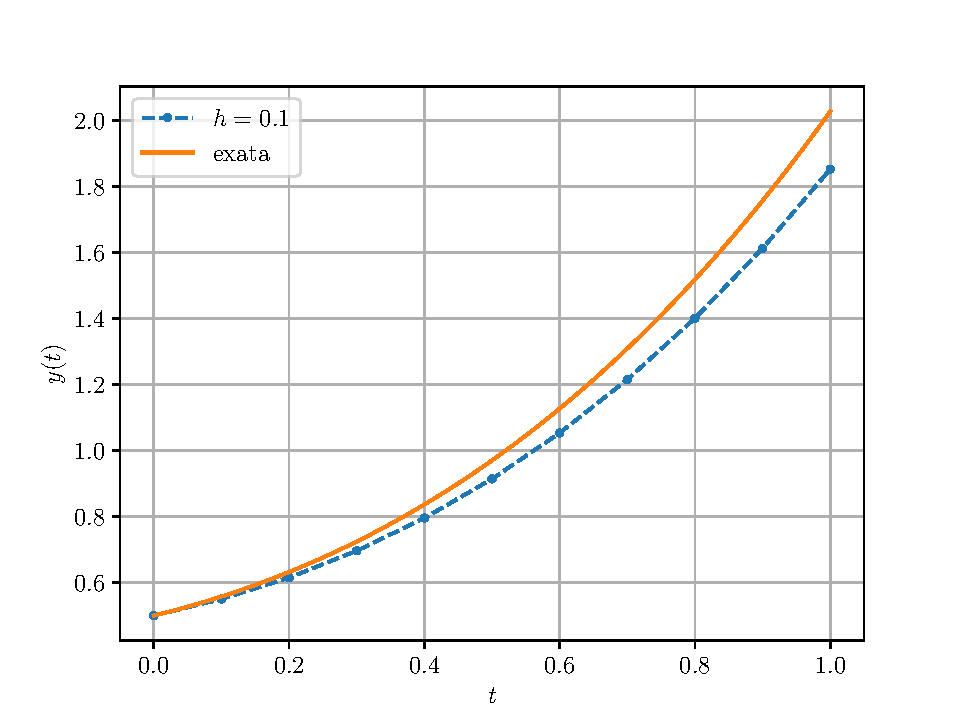
\includegraphics[width=\textwidth]{./cap_pvi/dados/fig_euler_ex0/fig}
  \caption{Esboço das soluções numérica (pontos) e analítica (linha) para o problema do Exemplo~\ref{cap_pvi_sec_euler:ex:euler_ex0}.}
  \label{fig:ex_Euler_1}
\end{figure}
\end{ex}

\begin{lstlisting}[caption=euler.py, label=cap_pvi_sec_euler:cod:euler]
def euler(f, t0, y0, h, n):
    t = np.empty(n+1)
    t[0] = t0
    y = np.empty(n+1)
    y[0] = y0
    for k in range(n):
        t[k+1] = t[k] + h
        y[k+1] = y[k] + h*f(t[k], y[k])
    return t, y
\end{lstlisting}

\subsection{Análise Numérica}

O Método de Euler com passo $h$ aplicado ao problema de valor inicial \eqref{cap_pvi_sec_euler:eq:pvi}, pode ser escrito da seguinte forma
\begin{subequations}\label{cap_pvi_sec_euler:eq:mps}\hleq
  \begin{align}
    \tilde{y}(t^{(0)}; h) &= y_0,\\
    \tilde{y}(t^{(k+1)}; h) &= \tilde{y}(t^{(k)}; h) + h\Phi(t^{(k)}, \tilde{y}(t^{(k)}); h),
  \end{align}
\end{subequations}
onde $\tilde{y}(t^{(k)})$ representa a aproximação da solução exata $y$ no tempo $t^{(k)}=t_0+ kh$, $k=0, 1, 2, \ldots$. Métodos que podem ser escritos dessa forma, são chamados de \hl{\emph{Métodos de Passo Simples}} (ou único). No caso específico do método de Euler, temos
\begin{equation}\hleq
  \Phi(t, y; h) := f(t, y(t)).
\end{equation}

Agora, considerando a solução exata $y$ de \eqref{cap_pvi_sec_euler:eq:pvi}, introduzimos
\begin{equation}\hleq
  \Delta(t, y; h) := \left\{
    \begin{array}{ll}
      \displaystyle\frac{y(t+h)-y(t)}{h} &, h\neq 0,\\
      f(t, y(t)) &, h=0,
    \end{array}\right.
\end{equation}

Com isso, vamos analisar o chamado \hl{\emph{erro de discretização local}}
\begin{equation}\hleq
  \tau(t, y; h) := \Delta(t, y; h) - \Phi(t, y; h),
\end{equation}
que \hl{estabelece uma medida quantitativa com que a solução exata $y(t)$ no tempo $t+h$ satisfaz a iteração de Euler}.

\subsubsection{Consistência}

\begin{defn}\normalfont{\hl{(Consistência.)}}\label{cap_pvi_sec_euler:defn:consistencia}
  Um \hl{método} de passo simples é dito ser \hl{consistente} quando
  \begin{equation}\hleq
    \lim_{h\to 0}\tau(t,y;h) = 0,
  \end{equation}
  ou, equivalentemente, quando
  \begin{equation}
    \lim_{h\to 0} \Phi(t, y; h) = f(t, y).
  \end{equation}
\end{defn}

\begin{obs}\normalfont{(Consistência do Método de Euler.)}
  Da Definição~\ref{cap_pvi_sec_euler:defn:consistencia}, temos que o \hl{Método de Euler é consistente}. De fato, temos
  \begin{align}
    \lim_{h\to 0} \tau(t, y; h) &= \lim_{h\to 0} \left(\Delta(t, y; h) - \Phi(t, y; h)\right)\\
                                &= \lim_{h\to 0} \left(\frac{y(t+h)-y(t)}{h} - f\left(t,y(t)\right)\right)\\
                                &= y'(t) - f\left(t, y(t)\right) = 0.
  \end{align}
\end{obs}

A \hl{\emph{ordem do erro de discretização local}} de um método de passo simples é dita ser $p$, quando
\begin{equation}\hleq
  \tau(t, y; h) = O(h^p),
\end{equation}
ou seja, quando
\begin{equation}
  \lim_{h\to 0} \frac{\tau(t, y; h)}{h^p} = C,
\end{equation}
para alguma constante $C$.

Para determinarmos a ordem do Método de Euler, tomamos a \hl{expansão em série de Taylor}{\taylor} da solução exata $y(t)$ em torno de $t$, i.e.
\begin{equation}\label{cap_pvi_sec_euler:eq:taylor}
  y(t+h) = y(t) + hy'(t) + \frac{h^2}{2}y''(t) + \frac{h^3}{6}y'''(t+\theta h),
\end{equation}
para algum $0<\theta<1$.
Como $y'(t)=f(t, y(t))$, temos
\begin{align}
  y''(t) &= \frac{d}{dt}f(t, y(t)) \\
         &= f_t(t, y) + f_y(t, y)y'\\
         &= f_t(t, y) + f_y(t, y)f(t, y).
\end{align}
Então, rearranjando os termos em \eqref{cap_pvi_sec_euler:eq:taylor}, obtemos
\begin{equation}\label{eq:pvi_delta_aux}
  \Delta(t, y; h) = f(t, y(t)) + \frac{h}{2}[f_t(t, y) + f_y(t, y)f(t, y)] + O(h^2).
\end{equation}
Portanto, para o método de Euler temos
\begin{align}
  \tau(t, y; h) &:= \Delta(t, y; h)-\Phi(t, y; h)\\
              &= \Delta(t, y; h) - f(t, y)\\
              &= \frac{h}{2}[f_t(t, y) + f_y(t, y)f(t, y)] + O(h^2)\\
              &= O(h).
\end{align}
Isto mostra que o \hl{Método de Euler é de ordem $1$}.

\subsubsection{Convergência}

A análise acima trata apenas da consistência do Método de Euler. Para analisarmos a \hl{convergência} de métodos de passo simples, definimos o \hl{\emph{erro de discretização global}}
\begin{equation}\hleq
  e(t; h_n) := \tilde{y}(t; h_n) - y(t),
\end{equation}
onde $\tilde{y}(t; h_n) \approx y(t)$ para $h_n := (t-t_0)/n$. Dizemos que o método é \hl{\emph{convergente}} quando
\begin{equation}\hleq
  \lim_{n\to \infty} e(t,h_n) = 0.
\end{equation}
Ainda, dizemos que o método tem \hl{erro de discretização global de ordem $p$} quando
\begin{equation}\hleq
  e(t,h_n) = O(h_n^p)
\end{equation}
para todo $t\in [t_0, t_f]$, $t_f > t_0$.

\begin{lema}\normalfont{(\cite[Cap. 7, Seção 7.2]{Stoer1993a})}\label{cap_pvi_sec_euler:lema:aux}
  Se a sequência $\left(\xi^{(k)}\right)_{k\in\mathbb{R}}$ satisfaz a estimativa
  \begin{equation}
    \left|\xi^{(k+1)}\right| \leq (1 + \delta)\left|\xi^{(k)}\right| + B,
  \end{equation}
  para dados $\delta > 0$ e $B\geq 0$, $k=0, 1, 2, \ldots$, então
  \begin{equation}
    \left|\xi^{(n)}\right| \leq e^{n\delta}\left|\xi^{(0)}\right| + \frac{e^{n\delta}-1}{\delta}B.
  \end{equation}
\end{lema}
\begin{dem}
  De forma iterativa, temos
  \begin{align}
    \left|\xi^{(1)}\right| &\leq (1 + \delta)\left|\xi^{(0)}\right| + B\\
    \left|\xi^{(2)}\right| &\leq (1 + \delta)\left|\xi^{(1)}\right| + B\\
                           &= (1+\delta)^2\left|\xi^{(0)}\right| + (1+\delta)B + B\\
                           &\vdots\\
    \left|\xi^{(k)}\right| &\leq (1 + \delta)^k\left|\xi^{(0)}\right| + B\sum_{k=0}^{k-1}(1+\delta)^k\\
                           &= (1 + \delta)^k\left|\xi^{(0)}\right| + B\frac{(1+\delta)^k-1}{\delta}.
  \end{align}
  Observando que $0<1+\delta\leq e^{\delta}$ para $\delta>-1$, concluímos que
  \begin{equation}
    \left|\xi^{(k)}\right| \leq e^{k\delta}\left|\xi^{(0)}\right| + \frac{e^{k\delta}-1}{\delta}B.
  \end{equation}
\end{dem}

\begin{teo}\normalfont{\hl{(Estimativa do Error Global.)}}\label{cap_pvi_sec_euler:teo:conv}
  Considere o PVI \eqref{cap_pvi_sec_euler:eq:pvi}, para $t_0 = a$, $y_0\in\mathbb{R}$. Suponha que $f$ é Lipschitz contínua em $y$
  \begin{equation}
    |f(t, y) - f(t, z)| \leq L|y - z|,
  \end{equation}
  para todo $(t,y)\in [a, b]\times\mathbb{R}$ e que exista $M>0$ tal que
  \begin{equation}
    |y''(t)| \leq M,
  \end{equation}
  para todo $t\in [a, b]$. Então, as iteradas do Método de Euler $y^{(k)} \approx y\left(t^{(k)}\right)$, $t^{(k)} = t_0 + kh$, $h > (b-a)/n$, $k=0, 1, 2, \dotsc, n+1$, satisfazem a seguinte \hl{\emph{estimativa do erro de discretização global}}
  \begin{equation}\label{cap_pvi_sec_euler:eq:est_errg}\hleq
    \left|y^{(k)} - y\left(t^{(k)}\right)\right| \leq \frac{hM}{2L}\left[e^{L\left(t^{(k)}-t_0\right)}-1\right].
  \end{equation}
\end{teo}
\begin{dem}
  Para $k=0$ o resultado é imediato. Agora, usamos o polinômio de Taylor
  \begin{equation}
    y\left(t^{(k+1)}\right) = y\left(t^{(k)}\right) + hf\left(t^{(k)}, y\left(t^{(k)}\right)\right) + \frac{h^2}{2}y''\left(\xi^{(k)}\right),
  \end{equation}
  onde $t^{(k)} \leq \xi^{(k)} \leq t^{(k+1)}$, $k=0, 1, 2, \ldots, n$. Já, as iteradas de Euler são
  \begin{equation}
    y^{(k+1)} = y^{(k)} + hf\left(t^{(k)}, y^{(k)}\right).
  \end{equation}
  Subtraindo esses equações, obtemos
  \begin{equation}
    \begin{aligned}
      y^{(k+1)} - y\left(t^{(k+1)}\right) &= y^{(k)} - y\left(t^{(k)}\right) \\
      &+ h\left[f\left(t^{(k)}, y^{(k)}\right) - f\left(t^{(k)}, y\left(t^{(k)}\right)\right)\right] - \frac{h^2}{2}y''\left(\xi^{(k)}\right)
    \end{aligned}
  \end{equation}
  Da hipótese de $f$ Lipschitz, temos
  \begin{equation}
    \begin{aligned}
      \left|y^{(k+1)} - y\left(t^{(k+1)}\right)\right| &\leq \left|y^{(k)} - y\left(t^{(k)}\right)\right| \\
      &+ hL\left|y^{(k)} - y\left(t^{(k)}\right)\right| + \frac{h^2}{2}\left|y''\left(\xi^{(k)}\right)\right|
    \end{aligned}
  \end{equation}
  Ou, ainda,
  \begin{equation}
    \left|y^{(k+1)} - y\left(t^{(k+1)}\right)\right| \leq (1 + hL)\left|y^{(k+1)} - y\left(t^{(k+1)}\right)\right| + \frac{h^2M}{2}.
  \end{equation}
  Do Lema \ref{cap_pvi_sec_euler:lema:aux}, temos
  \begin{equation}
    \left|y^{(k+1)} - y\left(t^{(k+1)}\right)\right| \leq \frac{h^2M}{2}\frac{e^{khL}-1}{hL},
  \end{equation}
  donde segue a estimativa do erro global \eqref{cap_pvi_sec_euler:eq:est_errg}.
\end{dem}

% \begin{teo}\normalfont{(\hl{Convergência}.)}\label{cap_pvi_sec_euler:teo:conv}
%   Considere o PVI \eqref{cap_pvi_sec_euler:eq:pvi}, para $t_0\in [a, b]$ e $y_0\in\mathbb{R}$. Seja $\Phi$ contínua em
%   \begin{equation}
%     G := \{(t, y, h): a\leq t\leq b, |y-y(t)|\leq\gamma, 0\leq|h|\leq h_0\},
%   \end{equation}
%   para $h_0>0$ e $\gamma>0$. Sejam também, $M, N$ constantes tais que
%   \begin{equation}
%     \left|\Phi(t, y; h) - \Phi(t, z; h)\right| \leq M|y - z|,
%   \end{equation}
%   para todas $(t, y; h), (t, z; h)\in G$. Se, ainda, para algum $p>0$ e para todo $t\in [a, b]$, $|h|\leq h_0$,
%   \begin{equation}\hleq
%     \left|\tau(t, y(t); h)\right| \leq N |h|^p,
%   \end{equation}
%   então existe $\overline{h}$, $0<\overline{h}<h_0$, tal que
%   \begin{equation}\hleq
%     |e(t; h_n)| \leq |h_n|^pN\frac{e^{M|t-t_0|}-1}{M},
%   \end{equation}
%   para todo $t\in [a, b]$ e para todo $h_n = (t-t_0)/n$, $n=1, 2, \ldots$, com $|h_n|\leq \overline{h}$.
% \end{teo}
% \begin{dem}
%   Seja
%   \begin{equation}
%     \tilde{\Phi}(t, y; h) := \left\{
%       \begin{array}{ll}
%         \Phi(t, y; h) &, (t, y, h)\in G,\\
%         \Phi(t, y(t)+\gamma; h) &, t\in [a, b], |h|\leq h_0, y\geq y(t)+\gamma,\\
%         \Phi(t, y(t)-\gamma; h) &, t\in [a, b], |h|\leq h_0, y\leq y(t)-\gamma,
%       \end{array}
%     \right.
%   \end{equation}
%   A função $\tilde{\Phi}$ é contínua em
%   \begin{equation}
%     \tilde{G} := \{(t, y; h): t\in [a, b], y\in\mathbb{R}, |h|\geq h_0\}
%   \end{equation}
%   e satisfaz
%   \begin{equation}\label{cap_pvi_sec_euler:eq:aux0}
%     \left|\tilde{\Phi}(t, y; h) - \tilde{\Phi}(t, z; h)\right| \leq M|y - z|,
%   \end{equation}
%   para todas $(t, y; h), (t, z; h)\in \tilde{G}$. Ainda, como $\tilde{\Phi}(t, y(t); h) = \Phi(t, y(t); h)$, também temos que
%   \begin{equation}\label{cap_pvi_sec_euler:eq:aux1}
%     |\Delta(t, y(t); h) - \tilde{\Phi}(t, y(t); h)| \leq N |h|^p,
%   \end{equation}
%   para $t\in [a, b]$ e $|h|\leq h_0$.

%   Sejam, $\tilde{y}^{(k)} := \tilde{y}\left(t^{(k)}; h\right)$, $t^{(k)} = t_0 + kh$, $\tilde{y}^{(0)} = y_0$:
%   \begin{align}
%     \tilde{y}^{(k+1)} = \tilde{y}^{(k)} + h\tilde{\Phi}\left(t^{(k)}, \tilde{y}^{(k)}; h\right),
%     y\left(t^{(k+1)}\right) = y\left(t^{(k)}\right) + h\Delta\left(t^{(k)}, y\left(t^{(k)}\right); h\right).
%   \end{align}
%   Definindo $\tilde{e}^{(k)} := \tilde{y}^{(k)} - y\left(t^{(k)}\right)$, obtemos a fórmula de recorrência
%   \begin{align}
%     \tilde{e}^{(k+1)} &= \tilde{e}^{(k)} + h\left[\tilde{\Phi}\left(t^{(k)}, \tilde{y}^{(k)}; h\right) - \Delta\left(t^{(k)}, y\left(t^{(k)}\right); h\right)\right]\\
%                       &= \tilde{e}^{(k)} + h\left[\tilde{\Phi}\left(t^{(k)}, \tilde{y}^{(k)}; h\right) - \tilde{\Phi}\left(t^{(k)}, y\left(t^{(k)}\right); h\right)\right]\\
%                       &+ h\left[\tilde{\Phi}\left(t^{(k)}, y\left(t^{(k)}\right); h\right) - \Delta\left(t^{(k)}, y\left(t^{(k)}\right); h\right)\right].\label{cap_pvi_sec_euler:eq:aux2}
%   \end{align}
%   Agora, de \eqref{cap_pvi_sec_euler:eq:aux0} e \eqref{cap_pvi_sec_euler:eq:aux1}, temos
%   \begin{align}
%     &\left|\tilde{\Phi}\left(t^{(k)}, \tilde{y}^{(k)}; h\right) - \tilde{\Phi}\left(t^{(k)}, y\left(t^{(k)}\right); h\right)\right| \leq M\left|\tilde{e}^{(k)}\right|\\
%     &\left|\Delta\left(t^{(k)}, y\left(t^{(k)}\right); h\right) - \tilde{\Phi}\left(t^{(k)}, y\left(t^{(k)}\right); h\right)\right| \leq N |h|^p
%   \end{align}
%   Portanto, de \eqref{cap_pvi_sec_euler:eq:aux2}, temos
%   \begin{equation}
%     \left|\tilde{e}^{(k+1)}\right| \leq \left(1 + |h|M\right)\left|\tilde{e}^{(k)}\right| + N |h|^{p+1}
%   \end{equation}
%   Então, do Lema \ref{cap_pvi_sec_euler:lema:aux}, temos
%   \begin{equation}\label{cap_pvi_sec_euler:eq:aux3}
%     \left|\tilde{e}^{(k)}\right| \leq N|h|^p\frac{e^{k|h|M}-1}{M}.
%   \end{equation}
%   Sejam, agora, $t\in [a, b]$, $t\neq t_0$ fixo e $h := h_n = (t-t_0)/n$, $n>0$. Então, $t^{(n)} = t_0 + nh = t$ e de \eqref{cap_pvi_sec_euler:eq:aux3} temos
%   \begin{equation}
%     \left|\tilde{e}\left(t, h_n\right)\right| \leq N|h_n|^p\frac{e^{M|t-t_0|}-1}{M},
%   \end{equation}
%   para todo $t\in [a, b]$, $|h_n|\leq h_0$. Uma vez que $|t-t_0|\leq |b-a|$ e $\gamma >0$, existe $\overline{h}$, $0<\overline{h}\leq h_0$, tal que $\left|\tilde{e}\left(t, h_n\right)\right| \leq \gamma$ para todo $t\in [a, b]$ e $|h_n|\leq \overline{h}$. Logo, para o método de passo simples \eqref{cap_pvi_sec_euler:eq:mps} gerado por $\Phi$, temos para $|h|\leq\overline{h}$ que
%   \begin{align}
%     &\tilde{y}^{(k)} = y^{(k)},\\
%     &\tilde{e}^{(k)} = e^{(k)},\\
%     &\tilde{\Phi}\left(t^{(k)}, \tilde{y}^{(k)}; h\right) = \Phi\left(t^{(k)}, \tilde{y}^{(k)}; h\right).
%   \end{align}
%   Concluímos que
%   \begin{equation}
%     \left|e\left(t, h_n\right)\right| \leq N|h_n|^p\frac{e^{M|t-t_0|}-1}{M},
%   \end{equation}
%   para todo $t\in [a, b]$ e $h_n = (t-t_0)/n$, $n=1, 2, \ldots$, com $|h_n|\leq \overline{h}$.
% \end{dem}

\begin{obs}\normalfont{\hl{(Convergência.)}}
  Do Teorema \ref{cap_pvi_sec_euler:teo:conv}, \hl{a ordem do erro de discretização global de um método de passo simples é igual a sua ordem do erro de discretização local}. Portanto, o \hl{Método de Euler é convergente e é de ordem $1$}.
\end{obs}

\begin{ex}\label{cap_pvi_sec_euler:ex:conv}
  Consideremos o seguinte problema de valor inicial
  \begin{subequations}
    \begin{align}
      &y' = y + 1, t>0\\
      &y(0) = 0.
    \end{align}
\end{subequations}
  Na Tabela~\ref{cap_pvi_sec_euler:tab:euler_conv}, temos as aproximações $\tilde{y}(1)$ de $y(1)$ computadas pelo Método de Euler com diferentes passos $h$. A solução analítica deste problema é $y(t) = e^{t}-1$.
 
  \begin{table}[h!]
    \centering
    \caption{Resultados referentes ao Exemplo~\ref{cap_pvi_sec_euler:ex:conv}.}
    \begin{tabular}{l|cc}
      $h$ & $\tilde{y}(1)$ & $|\tilde{y}(1)-y(1)|$\\\hline
      $10^{-1}$ & $1.59374$ & $1.2\E-1$ \\
      $10^{-2}$ & $1.70481$ & $1.3\E-2$ \\
      $10^{-3}$ & $1.71692$ & $1.4\E-3$ \\
      $10^{-5}$ & $1.71827$ & $1.4\E-5$ \\
      $10^{-7}$ & $1.71828$ & $1.4\E-7$ \\
      $10^{-9}$ & $1.71828$ & $1.4\E-9$ \\\hline
    \end{tabular}
    \label{cap_pvi_sec_euler:tab:euler_conv}
  \end{table}
\end{ex}

\subsubsection{Erros de Arredondamento}

O Teorema \ref{cap_pvi_sec_euler:teo:conv} não leva em consideração os erros de arredondamento. Levando em conta esses erros, a iteração do método de Euler tem a forma
\begin{subequations}\label{cap_pvi_sec_euler:eq:euler_errarr}
  \begin{align}
    &\tilde{y}^{(0)} = y_0 + \delta^{(k)},\\
    &\tilde{y}^{(k+1)} = \tilde{y}^{(k)} + hf\left(t^{(k)}, \tilde{y}^{(k)}\right) + \delta^{(k+1)},
  \end{align}
\end{subequations}
onde $\delta^{(k)}$ é o erro devido a arredondamentos na $k$-ésima iterada, $t^{(k)} = t_0 + hk$, $k=0, 1, 2, \dotsc, n$. Assumindo as hipóteses do Teorema \ref{cap_pvi_sec_euler:teo:conv}, podemos mostrar a seguinte estimativa de erro global
\begin{equation}\label{cap_pvi_sec_euler:eq:euler_errarr_est}\hleq
  \begin{aligned}
    \left|\tilde{y}^{(k+1)} - y\left(t^{(k+1)}\right)\right| &\leq \frac{1}{L}\left(\frac{hM}{2} + \frac{\delta}{h}\right)\left[e^{L\left(t^{(k)}-t_0\right)}-1\right]\\
    &+ |\delta_0|e^{L\left(t^{(k)}-t_0\right)},
\end{aligned}
\end{equation}
para $\delta^{(k)} < \delta$, $k=0, 1, 2, \dotsc, n$.

\subsection*{Exercícios}

\begin{exer}
  O problema de valor inicial
  \begin{subequations}
    \begin{align}
      &y' = \pi\left[\cos^2(\pi t) - \sen^2(\pi t)\right],\quad t>0\\
      &y(0) = 0.
    \end{align}
  \end{subequations}
  tem solução analítica $y(t) = \sen(\pi t)\cos(\pi t)$. Compute a aproximação $\tilde{y}(1) \approx y(1)$ pelo Método de Euler com passo $h=10^{-1}$ e forneça o erro $e(1, h) := \tilde{y}(1, h) - y(1)$.
\end{exer}
\begin{resp}
  $\tilde{y}(1.5) = 3.14159\E-1$, $e(1, h) = 3.1E-01$
\end{resp}

\begin{exer}
  Use o Método de Euler para computar a solução de
  \begin{subequations}
    \begin{align}
      &y' = e^{2t} - 2y,\quad 0 < t\leq 1,\\
      &y(0) = 0.
    \end{align}
  \end{subequations}
  Escolha um passo $h$ adequado de forma que $y(1)$ seja computado com precisão de $5$ dígitos significativos.
\end{exer}
\begin{resp}
  $h=10^{-6}$, $\tilde{y}(1) = 1.8134\E+0$
\end{resp}

\begin{exer}
  Considere o seguinte problema de valor inicial
  \begin{subequations}
    \begin{align}
      &y' + e^{-y^2+1} = 2,\quad t>1,\\
      &y(1) = -1.
    \end{align}
\end{subequations}
Use o método de Euler para computar o valor aproximado de $y(2)$ com precisão de $6$ dígitos significativos.
\end{exer}
\begin{resp}
  $-5.58858\E-1$
\end{resp}

\begin{exer}
  Use o Método de Euler para computar a solução de
  \begin{subequations}
    \begin{align}
      &y' = -30y,\quad 0 < t\leq 1,\\
      &y(0) = \frac{1}{3}
    \end{align}
  \end{subequations}
  A solução analítica é $y(t) = \frac{1}{3}e^{-30t}$. Compute a solução aproximação $\tilde{y}(1)$ e o erro $|\tilde{y}(1) - y(1)|$ usando o passo $h=10^{-1}$. O erro obtido está de acordo com a estimativa \eqref{cap_pvi_sec_euler:eq:est_errg}?
\end{exer}
\begin{resp}
  $|\tilde{y}(1) - y(1)| = 3.4\E+2$. Dica: verifique as hipóteses do Teorema \ref{cap_pvi_sec_euler:teo:conv}.
\end{resp}

\subsubsection{Análise Numérica}

\begin{exer}
  Mostre que se $\delta>-1$, então $0 < 1+\delta \leq e^{\delta}$.
\end{exer}
\begin{resp}
  Dica: use o polinômio de Taylor de grau 2 de $e^\delta$.
\end{resp}

\begin{exer}
  Seja dado um PVI \eqref{cap_pvi_sec_euler:eq:pvi}, $t_0\leq t \leq t_f$. Sejam $\tilde{y}^{(k)}$, $k=0, 1, 2, \dotsc, n$, as aproximações computadas conforme em \eqref{cap_pvi_sec_euler:eq:euler_errarr}, com $\delta^{(k)} < \delta$. Assumindo as mesmas hipóteses do Teorema \ref{cap_pvi_sec_euler:teo:conv}, mostre a estimativa de erro global \eqref{cap_pvi_sec_euler:eq:euler_errarr_est}.
\end{exer}
\begin{resp}
  Dica: estude a demonstração do Teorema \ref{cap_pvi_sec_euler:teo:conv}.
\end{resp}

\begin{exer}
  Assumindo um erro de arredondamento máximo de $\delta > 0$, use \eqref{cap_pvi_sec_euler:eq:euler_errarr_est} para obter uma estimativa para a melhor escolha de $h$.
\end{exer}
\begin{resp}
  $h = \sqrt{2\delta/M}$. Dica: Encontre o mínimo de $E(h) := M/2 + \delta/h^2$.
\end{resp}


\section{Métodos de Runge-Kutta}\label{cap_pvi_sec_RK}

\begin{flushleft}
  [[tag:revisar]]
\end{flushleft}

Os métodos de Runge-Kutta de $s$-estágios são métodos de passo simples da seguinte forma
\begin{equation}
  y^{(i+1)} = y^{(i)} + h(c_1k_1 + \cdots + c_sk_s)
\end{equation}
onde
\begin{align}
  k_1 &:= f(t^{(i)},y^{(i)}),\\
  k_2 &:= f(t^{(i)}+\alpha_2h,y^{(i)}+h\beta_{21}k_1),\\
  k_3 &:= f(t^{(i)}+\alpha_3h,y^{(i)}+h(\beta_{31}k_1+\beta_{32}k_2)),\\
      &~~\vdots\\
  k_s &:= f(t^{(i)}+\alpha_sh,y^{(i)}+h(\beta_{s1}k_1+\cdots+\beta_{s,s-1}k_{s-1})),
\end{align}
$t^{(i)}=t_0+(i-1)h$ e $y^{(1)}=y_0$.

Na sequência, discutimos alguns dos métodos de Runge-Kutta usualmente utilizados. Pode-se encontrar uma lista mais completa em~\cite[Cap. 8, Seç. 3.2]{Isaacson1994a}.

\subsection{Métodos de Runge-Kutta de ordem 2}

\begin{flushleft}
  [[tag:revisar]]
\end{flushleft}

Precisamos apenas de $2$ estágios para obtermos métodos de Runge-Kutta de ordem 2. Portanto, assumimos
\begin{align}
  y^{(i+1)} = y^{(i)} &+ h\left[c_1f(t^{(i)},y^{(i)}) \right.\nonumber\\
  &\left. + c_2f(t^{(i)}+\alpha_2h,y^{(i)}+h\beta_{21}f(t^{(i)},y^{(i)}))\right].\label{eq:rk_2_aux}
\end{align}
Neste caso, o erro de discretização local é dado por
\begin{equation}
  \tau(t,y;h) = \Delta(t,y;h) - \Phi(t,y;h),
\end{equation}
onde, da equação~\eqref{eq:pvi_delta_aux} temos
\begin{equation}\label{eq:pvi_delta_aux2}
  \Delta(t,y;h) = f(t,y(t)) + \frac{h}{2}[f_t(t,y) + f_y(t,y)f(t,y)] + O(h^2)
\end{equation}
e de~\eqref{eq:rk_2_aux}
\begin{equation}
  \Phi(t,y;h) = c_1f(t,y) + c_2f(t+\alpha_2h,y+h\beta_{21}f(t,y))
\end{equation}
Agora, tomando a expansão de série de Taylor em torno de $t$ de $\Phi(t,y;h)$, temos
\begin{align}\label{eq:pvi_phi_aux2}
  \Phi(t,y;h) = (c_1+c_2)f(t,y) &+ c_2h[\alpha_2f_t(t,y) \nonumber\\
  &+\beta_{21}f_y(t,y)f(t,y)) + O(h^2).
\end{align}
Então, por comparação de \eqref{eq:pvi_delta_aux2} e \eqref{eq:pvi_phi_aux2}, temos
\begin{align}
  c_1&+c_2 = 1\\
  c_2&\alpha_2 = \frac{1}{2}\\
  c_2&\beta_{21} = \frac{1}{2}.
\end{align}
Assim sendo, temos mais de uma solução possível.

\subsubsection{Método do ponto médio}

\begin{flushleft}
  [[tag:revisar]]
\end{flushleft}

O método do ponto médio é um método de Runge-Kutta de ordem $2$ proveniente da escolha de coeficientes
\begin{equation}
  c_1 = 0, \quad c_2 = 1, \quad \alpha_2 = \frac{1}{2},\quad \beta_{21}=\frac{1}{2}.
\end{equation}
Logo, a iteração do método do ponto médio é
\begin{align}
  y^{(1)} &= y_0\\
  y^{(i+1)} &= y^{(i)} + hf\left(t^{(i)}+\frac{h}{2},y^{(i)}+\frac{h}{2}f(t^{(i)},y^{(i)})\right).
\end{align}

\begin{ex}\label{ex:ponto_medio_1}
  Consideremos o seguinte problema de valor inicial
  \begin{align}
    y' - y &= \sen(t), t>0\\
    y(0) &= \frac{1}{2}.
  \end{align}
  Na Tabela~\ref{tab:ex_ponto_medio_1}, temos as aproximações $\tilde{y}(1)$ de $y(1)$ computadas pelo método do ponto médio com diferentes passos $h$.
 
  \begin{table}[h!]
    \centering
    \begin{tabular}{l|cc}
      $h$ & $\tilde{y}(1)$ & $|\tilde{y}(1)-y(1)|$\\\hline
      $10^{-1}$ & $2,02175$ & $5,6\E-03$ \\
      $10^{-2}$ & $2,02733$ & $6,0\E-05$ \\
      $10^{-3}$ & $2,02739$ & $6,1\E-07$ \\
      $10^{-4}$ & $2,02740$ & $6,1\E-09$ \\
      $10^{-5}$ & $2,02737$ & $2,9\E-05$ \\\hline
    \end{tabular}
    \caption{Resultados referentes ao Exemplo~\ref{ex:ponto_medio_1}.}
    \label{tab:ex_ponto_medio_1}
  \end{table}

% \ifisoctave
% Os resultados mostrados na Tabela~\ref{tab:ex_ponto_medio_1} podem ser computados no \verb+GNU Octave+ com o auxílio do seguinte código:
% \begin{verbatim}
% f = @(t,y) y+sin(t);

% h=1e-1;
% n=round(1/h+1);
% t=zeros(n,1);
% y=zeros(n,1);

% t(1)=0;
% y(1)=0.5;

% for i=1:n-1
%   t(i+1) = t(i)+h;
%   y(i+1)=y(i)+h*f(t(i)+h/2,y(i)+h/2*f(t(i),y(i)));
% endfor

% ya = @(t) exp(t)-sin(t)/2-cos(t)/2;
% printf("%1.5E %1.1E\n",y(n),abs(y(n)-ya(1)))
% \end{verbatim}
% \fi
\end{ex}

\subsubsection{Método de Euler modificado}

\begin{flushleft}
  [[tag:revisar]]
\end{flushleft}

O método de Euler modificado é um método de Runge-Kutta de ordem $2$ proveniente da escolha de coeficientes
\begin{equation}
  c_1 = \frac{1}{2}, \quad c_2 = \frac{1}{2}, \quad \alpha_2 = 1,\quad \beta_{21}=1.
\end{equation}
Logo, a iteração do método de Euler modificado é
\begin{align}
  y^{(1)} &= y_0\\
  y^{(i+1)} &= y^{(i)} + \frac{h}{2}\left[f(t^{(i)},y^{(i)}) + f(t^{(i)}+h,y^{(i)}+hf(t^{(i)},y^{(i)})\right].
\end{align}

\begin{ex}\label{ex:Euler_modificado_1}
  Consideremos o seguinte problema de valor inicial
  \begin{align}
    y' - y &= \sen(t), t>0\\
    y(0) &= \frac{1}{2}.
  \end{align}
  Na Tabela~\ref{tab:ex_Euler_modificado_1}, temos as aproximações $\tilde{y}(1)$ de $y(1)$ computadas pelo método de Euler modificado com diferentes passos $h$.
 
  \begin{table}[h!]
    \centering
    \begin{tabular}{l|cc}
      $h$ & $\tilde{y}(1)$ & $|\tilde{y}(1)-y(1)|$\\\hline
      $10^{-1}$ & $2,02096$ & $6,4\E-03$ \\
      $10^{-2}$ & $2,02733$ & $6,9\E-05$ \\
      $10^{-3}$ & $2,02739$ & $6,9\E-07$ \\
      $10^{-4}$ & $2,02740$ & $6,9\E-09$ \\
      $10^{-5}$ & $2.02737$ & $2,9\E-05$ \\\hline
    \end{tabular}
    \caption{Resultados referentes ao Exemplo~\ref{ex:Euler_modificado_1}}
    \label{tab:ex_Euler_modificado_1}
  \end{table}

% \ifisoctave
% Os resultados mostrados na Tabela~\ref{tab:ex_Euler_modificado_1} podem ser computados no \verb+GNU Octave+ com o auxílio do seguinte código:
% \begin{verbatim}
% f = @(t,y) y+sin(t);

% h=1e-1;
% n=round(1/h+1);
% t=zeros(n,1);
% y=zeros(n,1);

% t(1)=0;
% y(1)=0.5;

% for i=1:n-1
%   t(i+1) = t(i)+h;
%   y(i+1)=y(i)+h*f(t(i),y(i));
%   y(i+1)=y(i)+h/2*(f(t(i),y(i))+f(t(i+1),y(i+1)));
% endfor

% ya = @(t) exp(t)-sin(t)/2-cos(t)/2;
% printf("%1.5E %1.1E\n",y(n),abs(y(n)-ya(1)))
% \end{verbatim}
% \fi
\end{ex}

\subsection{Método de Runge-Kutta de ordem $4$}

\begin{flushleft}
  [[tag:revisar]]
\end{flushleft}

Um dos métodos de Runge-Kutta mais empregados é o seguinte método de ordem $4$:
\begin{equation}
  y^{(i+1)} = y^{(i)} + \frac{h}{6}(k_1 + 2k_2 + 2k_3 + k_4),
\end{equation}
onde
\begin{align}
  k_1 &:= f(t^{(i)},y^{(i)}),\\
  k_2 &:= f(t^{(i)}+h/2,y^{(i)}+hk_1/2),\\
  k_3 &:= f(t^{(i)}+h/2,y^{(i)}+hk_2/2),\\
  k_4 &:= f(t^{(i)}+h,y^{(i)}+hk_3),
\end{align}
$t^{(i)}=t_0+(i-1)h$ e $y^{(1)}=y_0$.

\begin{ex}\label{ex:RK4_1}
  Consideremos o seguinte problema de valor inicial
  \begin{align}
    y' - y &= \sen(t), t>0\\
    y(0) &= \frac{1}{2}.
  \end{align}
  Na Tabela~\ref{tab:ex_RK4_1}, temos as aproximações $\tilde{y}(1)$ de $y(1)$ computadas pelo método de Runge-Kutta de quarta ordem com diferentes passos $h$.
 
  \begin{table}[h!]
    \centering
    \begin{tabular}{l|cc}
      $h$ & $\tilde{y}(1)$ & $|\tilde{y}(1)-y(1)|$\\\hline
      $10^{-1}$ & $2,02739$ & $2,8\E-06$ \\
      $10^{-2}$ & $2,02740$ & $3,1\E-10$ \\
      $10^{-3}$ & $2,02740$ & $3,0\E-14$ \\
      $10^{-4}$ & $2,02740$ & $4,4\E-14$ \\\hline
    \end{tabular}
    \caption{Resultados referentes ao Exemplo~\ref{ex:RK4_1}}
    \label{tab:ex_RK4_1}
  \end{table}

% \ifisoctave
% Os resultados mostrados na Tabela~\ref{tab:ex_RK4_1} podem ser computados no \verb+GNU Octave+ com o auxílio do seguinte código:
% \begin{verbatim}
% f = @(t,y) y+sin(t);

% h=1e-4;
% n=round(1/h+1);
% t=zeros(n,1);
% y=zeros(n,1);

% t(1)=0;
% y(1)=0.5;

% for i=1:n-1
%   t(i+1) = t(i)+h;
%   k1 = h*f(t(i),y(i));
%   k2 = h*f(t(i)+h/2,y(i)+k1/2);
%   k3 = h*f(t(i)+h/2,y(i)+k2/2);
%   k4 = h*f(t(i)+h,y(i)+k3);
%   y(i+1)=y(i)+(k1+2*k2+2*k3+k4)/6;
% endfor

% ya = @(t) exp(t)-sin(t)/2-cos(t)/2;
% printf("%1.5E %1.1E\n",y(n),abs(y(n)-ya(1)))
% \end{verbatim}
% \fi
\end{ex}

\subsection*{Exercícios}

\begin{flushleft}
  [[tag:revisar]]
\end{flushleft}

\begin{exer}
  Considere o seguinte problema de valor inicial
  \begin{align}
    y' &+ e^{-y^2+1} = 2,\quad t>1,\\
    y(1) &= -1.
  \end{align}
Use os seguintes métodos de Runge-Kutta com passo $h=0,1$ para computar o valor aproximado de $y(2)$:
\begin{enumerate}[a)]
\item método do ponto médio.
\item método de Euler modificado.
\item método de Runge-Kutta de ordem $4$.
\end{enumerate}
\end{exer}
\begin{resp}
  % \ifisoctave 
  % \href{https://github.com/phkonzen/notas/blob/master/src/MatematicaNumerica/cap_pvi/dados/exer_RK_pvi1/exer_RK_pvi1.m}{Código.} 
  % \fi
  a)~$-6,00654\E-1$; b)~$-6,00703\E-1$; c)~$-5,99608\E-1$
\end{resp}

\section{Método adaptativo com controle de erro}\label{cap_pvi_met_adap}

\begin{flushleft}
  [[tag:revisar]]
\end{flushleft}

Consideremos um problema de valor inicia
\begin{align}
  y'(t) &= f(t,y(t)),\quad t>t_0,\\
  y(t_0) &= y_0.
\end{align}
e um método de passo simples
\begin{align}
  y^{(1)} &= y_0,\\
  y^{(i+1)}(h^{(i+1)}) &= y^{(i)} + h^{(i+1)}\Phi(t^{(i)},y^{(i)};h^{(i+1)}),
\end{align}
com $t^{(i)} = t_0 + (i-1)h^{(i)}$. Nesta seção, discutiremos uma estimava para o maior valor de $h^{(i+1)}$ tal que o erro de discretização global $e(t^{(i+1)};h^{(i+1)})$ seja controlado por uma dada tolerância $TOL$, i.e.
\begin{equation}\label{eq:pvi_erro_aux1}
  |e(t^{(i+1)};h^{(i+1)})| := |y^{(i+1)}(h^{(i+1)}) - y(t^{(i+1)})| \approx TOL.
\end{equation}

Para um método de ordem $h^p$, pode-se mostrar que (veja, \cite[Cap. 7, Seç. 7.2]{Isaacson1994a})
\begin{equation}\label{eq:pvi_erro_aux0}
  y^{(i+1)}(h^{(i+1)}) = y(t^{(i+1)}) + e_p(t^{(i+1)})(h^{(i+1)})^p,
\end{equation}
onde $e(t^{(i+1)})$ é uma função apropriada. Então, assumindo que $e(t^{(i)};h^{(i)})=0$, temos
\begin{equation}\label{eq:pvi_erro_aux2}
  e_p(t^{(i+1)}) = h^{(i+1)}e_p'(t^{(i)})
\end{equation}
e, portanto, para termos \eqref{eq:pvi_erro_aux1} impomos que
\begin{equation}\label{eq:pvi_erro_aux4}
  |(h^{(i+1)})^{p+1}e_p'(t^{(i)})| = TOL.
\end{equation}
Daí, se obtermos uma aproximação para $e_p'(t^{(i)})$ teremos uma aproximação para o passo $h^{(i+1)}$.

Para estimarmos $e_p(t^{(i+1)})$, observamos que de \eqref{eq:pvi_erro_aux0} temos
\begin{equation}
  y^{(i+1)}\left(\frac{h^{(i+1)}}{2}\right) = y(t^{(i+1)}) + e_p(t^{(i+1)})\frac{(h^{(i+1)})^p}{2^p}
\end{equation}
e, então, subtraindo esta de \eqref{eq:pvi_erro_aux0} temos
\begin{equation}
  y^{(i+1)}(h^{(i+1)}) - y^{(i+1)}\left(\frac{h^{(i+1)}}{2}\right) = e_p(t^{(i+1)})\left(\frac{h^{(i+1)}}{2}\right)^p(2^p-1),
\end{equation}
donde
\begin{equation}
  e_p(t^{(i+1)})\left(\frac{h^{(i+1)}}{2}\right)^p = \frac{y^{(i+1)}(h^{(i+1)}) - y^{(i+1)}\left(\frac{h^{(i+1)}}{2}\right)}{2^p-1}.
\end{equation}
Daí, de \eqref{eq:pvi_erro_aux2}, obtemos
\begin{equation}
  e_p'(t^{(i)})h^{(i+1)}\left(\frac{h^{(i+1)}}{2}\right)^p = \frac{y^{(i+1)}(h^{(i+1)}) - y^{(i+1)}\left(\frac{h^{(i+1)}}{2}\right)}{2^p-1},
\end{equation}
o que nos fornece a seguinte aproximação de $e_p'(t^{(i)})$
\begin{equation}
  e_p'(t^{(i)}) = \frac{1}{(h^{(i+1)})^{p+1}}\frac{2^p}{2^p-1}\left[y^{(i+1)}(h^{(i+1)}) - y^{(i+1)}\left(\frac{h^{(i+1)}}{2}\right)\right].
\end{equation}

Assim sendo, de \eqref{eq:pvi_erro_aux4} temos que o passo $h^{(i+1)}$ apropriado é tal que
\begin{equation}\label{eq:pvi_passo_est}
  \frac{2^p}{2^p-1}\left|y^{(i+1)}(h^{(i+1)}) - y^{(i+1)}\left(\frac{h^{(i+1)}}{2}\right)\right| \approx TOL.
\end{equation}

Com base nesta estimativa podemos propor o seguinte método de passo adaptativo. Partindo de uma escolha arbitrária de $h$, computamos $y^{(i+1)}(h)$ e $y^{(i+1)}(h/2)$ de  $y^{(i)}$. Então, enquanto
\begin{equation}
  \frac{2^p}{2^p-1}\left|y^{(i+1)}(h) - y^{(i+1)}\left(\frac{h}{2}\right)\right| > TOL,
\end{equation}
tomamos sucessivas divisões de $h$ por $2$, até satisfazermos \eqref{eq:pvi_passo_est}. Obtido o $h$ que satisfaz \eqref{eq:pvi_passo_est}, temos computado $y^{(i+1)}$ com $h^{(i+1)}=h$.

\begin{ex}\label{ex:Euler_adap}
  Consideremos o seguinte problema de valor inicial
  \begin{align}
    y' - y &= \sen(t), t>0\\
    y(0) &= \frac{1}{2}.
  \end{align}
  A Figura~\ref{fig:ex_Euler_adap} mostra a comparação entre $y(t)$ e a solução numérica obtida da aplicação do método de Euler com passo adaptativo. No método, utilizamos o passo inicial $h^{(1)}=0,1$ e tolerância $TOL=10^{-4}$. Ao compararmos esta figura com a Figura~\eqref{fig:ex_Euler_1} fica evidente o controle do erro.

  \begin{figure}[h!]
    \centering
    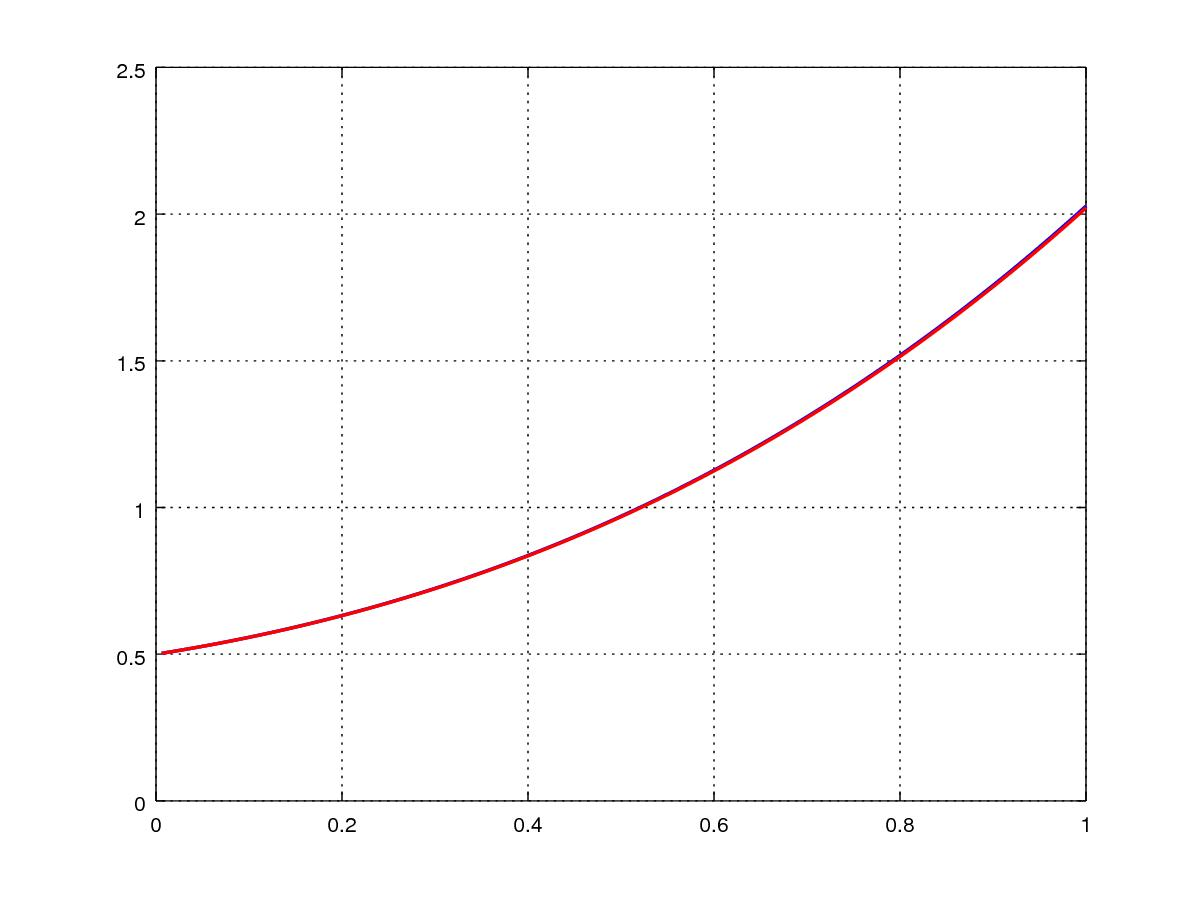
\includegraphics[width=0.8\textwidth]{./cap_pvi/dados/ex_Euler_adap/ex_Euler_adap}
    \caption{Resultados referentes ao Exemplo~\ref{ex:Euler_adap}.}
    \label{fig:ex_Euler_adap}
  \end{figure}

% \ifisoctave
% O algoritmo utilizado neste exemplo pode ser implementado no \verb+GNU Octave+ com o seguinte código:
% \begin{verbatim}
% f = @(t,y) y+sin(t);

% TOL=1e-4;
% h=1e-1;
% tf=1;

% t0=0;
% y0=0.5;

% t=[];
% y=[];

% c=1;
% do

%   h = min(h,tf-t0);
 
%   do
%     #passo h
%     y1=y0+h*f(t0,y0);
%     #passo h/2
%     y2=y0+h/2*f(t0,y0);
%     y2=y2+h/2*f(t0+h/2,y2);
%     #verifica TOL
%     est = 2*abs(y1-y2);
%     if (est > TOL)
%       h/=2;
%       if (h<1e-8)
%         error("h muito pequeno")
%       endif
%     else
%       t0+=h;
%       y0=y2;
      
%       t(c)=t0;
%       y(c)=y0;
%       c+=1;
%     endif
%   until ((est <= TOL))
  
% until (abs(t0-tf)<1e-14)

% ya = @(t) exp(t)-sin(t)/2-cos(t)/2;
% printf("%1.1E %1.5E %1.1E\n",t0,y0,abs(y0-ya(1)))

% plot(t,ya(t),'b-',t,y,'r-');grid
% \end{verbatim}
% \fi

\end{ex}

\subsection*{Exercícios}

\begin{flushleft}
  [[tag:revisar]]
\end{flushleft}

\begin{exer}
  Considere o seguinte problema de valor inicial
  \begin{align}
    y' &+ e^{-y^2+1} = 2,\quad t>1,\\
    y(1) &= -1.
  \end{align}
Use o método de Euler com passo adaptativo para computar o valor aproximado de $y(2)$. Para tanto, utilize o passo inicial $h=0,1$ e a tolerância de $TOL=10^{-4}$.
\end{exer}
\begin{resp}
  % \ifisoctave 
  % \href{https://github.com/phkonzen/notas/blob/master/src/MatematicaNumerica/cap_pvi/dados/exer_Euler_adap/exer_Euler_adap.m}{Código.} 
  % \fi
  $-5.99240\E-1$
\end{resp}


\section{Métodos de passo múltiplo}\label{cap_pvi_sec_passo_mult}

\begin{flushleft}
  [[tag:revisar]]
\end{flushleft}

Dado um problema de valor inicial
\begin{align}
  y'(t) &= f(t,y(t)),\quad t>t_0,\\
  y(t_0) &= y_0.
\end{align}
temos
\begin{equation}
  y(t) = y(t_0) + \int_{t_0}^t f(s,y(s))\,ds.
\end{equation}
De forma mais geral, consideramos uma partição uniforme no tempo $\{t_0=t^{(1)} < t^{(2)} < \cdots < t^{(i)} < \cdots < t^{(n)}=t_f\}$, onde $t_f$ é um determinado tempo para o qual queremos computar uma aproximação para $y(t_f)$. Também, denotamos o passo no tempo por $h=(t_f-t_0)/n$. Com isso, a solução $y(t)$ satisfaz
\begin{equation}
  y\left(t^{(i+k)}\right) = y\left(t^{(i-j)}\right) + \int_{t^{(i-j)}}^{t^{(i+k)}} f(s,y(s))\,ds.
\end{equation}
A ideia é, então, aproximar a integral acima por uma quadratura numérica.

Seguindo as regras de Newton-Cotes (veja, Cap.~\ref{cap_integr} Seç.~\ref{cap_integr_sec_NC}), escolhemos os nodos da quadratura como $x_l = t^{(i-l+1)}$, $l = 1, 2, \dotsc, m$, e, então
\begin{equation}
  \int_{t^{(i-j)}}^{t^{i+k}} f(x,y(x))\,dx \approx \sum_{l=1}^{m} f\left(x_l,y(x_l)\right)w_l,
\end{equation}
e
\begin{equation}
  w_l = \int_{t^{(i-j)}}^{t^{(i+k)}} \prod_{\overset{p=1}{p\neq l}}^m \frac{x-x_p}{x_l-x_p}\,dx.
\end{equation}
Agora, fazendo a mudança de variável $u=(x-t^{(i)})/h$, obtemos
\begin{equation}
  w_l = h\int_{-j}^{k} \prod_{\overset{p=1}{p\neq l}}^m \frac{u+p-1}{-l+p}\,du
\end{equation}
Assim sendo, temos o seguinte esquema numérico
\begin{equation}
  y^{(i+k)} = y^{(i-j)} + h\sum_{l=1}^m c_{l}f(t^{(i-l+1)},y^{(i-l+1)}),\label{eq:mult_passo_iter}
\end{equation}
onde
\begin{equation}
  c_l = \int_{-j}^{k} \prod_{\overset{p=1}{p\neq l}}^m \frac{s+p-1}{-l+p}\,ds.\label{eq:mult_passo_pesos}
\end{equation}

Diferentes escolhas de $j$, $k$ e $m$ não fornecem diferentes métodos. Observamos, ainda, que a ordem de um tal método de passo múltiplo é determinada pela ordem de truncamento da quadratura numérica usada (veja, por exemplo, \cite[Cap. 5, Seç. 5.6]{Burden2015a}).

\subsection{Métodos de Adams-Bashforth}\index{método de Adams-Bashforth}

\begin{flushleft}
  [[tag:revisar]]
\end{flushleft}

Métodos de Adams-Bashforth são métodos de passo múltiplo obtidos ao escolhermos $j=0$ e $k=1$ no esquema numérico~\eqref{eq:mult_passo_iter}. Com isso, ao escolhermos $m$ obtemos um método de ordem $O(h^{m})$~\cite[Cap. 5, Seç. 5.6]{Burden2015a}.

\subsubsection{Método de Adams-Bashforth de ordem 2}

\begin{flushleft}
  [[tag:revisar]]
\end{flushleft}

Tomando $m=2$ em \eqref{eq:mult_passo_pesos}, temos
\begin{equation}
  c_1 = \int_0^1 s+1\,ds = \frac{3}{2}
\end{equation}
e
\begin{equation}
  c_2 = \int_0^1 -s\,ds = -\frac{1}{2}.
\end{equation}
Então, de \eqref{eq:mult_passo_iter} temos a iteração do \emph{método de Adams-Bashforth de $2$ passos}:
\begin{align}
  y^{(1)} &= y_0,\\
  y^{(i+1)} &= y^{(i)} + \frac{h}{2}\left[3f(t^{(i)},y^{(i)}) - f(t^{(i-1)},y^{(i-1)})\right],
\end{align}
com $t^{(i)} = t_0 + (i-1)h$.

\begin{ex}\label{ex:AB2}
  Consideremos o seguinte problema de valor inicial
  \begin{align}
    y' - y &= \sen(t), t>0\\
    y(0) &= \frac{1}{2}.
  \end{align}
  Na Tabela~\ref{tab:ex_AB2}, temos as aproximações $\tilde{y}(1)$ de $y(1)$ computadas pelo método de Adams-Bashforth de $2$ passos. Como este método é de ordem $2$, escolhemos inicializá-lo pelo método do ponto médio, de forma a mantermos a consistência.
 
  \begin{table}[h!]
    \centering
    \begin{tabular}{l|cc}
      $h$ & $\tilde{y}(1)$ & $|\tilde{y}(1)-y(1)|$\\\hline
      $10^{-1}$ & $2,01582$ & $1,2\E-02$ \\
      $10^{-2}$ & $2,02727$ & $1,3\E-04$ \\
      $10^{-3}$ & $2,02739$ & $1,3\E-06$ \\
      $10^{-4}$ & $2,02740$ & $1,3\E-08$ \\
      $10^{-5}$ & $2,02740$ & $1,3\E-10$ \\\hline
    \end{tabular}
    \caption{Resultados referentes ao Exemplo~\ref{ex:AB2}}
    \label{tab:ex_AB2}
  \end{table}

% \ifisoctave
% Os resultados mostrados na Tabela~\ref{tab:ex_AB2} podem ser computados no \verb+GNU Octave+ com o auxílio do seguinte código:
% \begin{verbatim}
% f = @(t,y) y+sin(t);

% h=1e-1;
% n=round(1/h+1);
% t=zeros(n,1);
% y=zeros(n,1);

% #c.i.
% t(1)=0;
% y(1)=0.5;

% #inicializacao
% t(2)=t(1)+h;
% y(2)=y(1)+h*f(t(1)+h/2,y(1)+h/2*f(t(1),y(1)));

% #iteracoes
% for i=2:n-1
%   t(i+1) = t(i)+h;
%   y(i+1)=y(i) + ...
%         h/2*(3*f(t(i),y(i))-f(t(i-1),y(i-1)));
% endfor

% ya = @(t) exp(t)-sin(t)/2-cos(t)/2;
% printf("%f %1.5E %1.1E\n",t(n),y(n),abs(y(n)-ya(1)))
% \end{verbatim}
% \fi
\end{ex}

\subsubsection{Método de Adams-Bashforth de ordem 3}

\begin{flushleft}
  [[tag:revisar]]
\end{flushleft}

Tomando $m=3$ em \eqref{eq:mult_passo_pesos} obtemos, de \eqref{eq:mult_passo_iter}, a iteração do \emph{método de Adams-Bashforth de $3$ passos}:
\begin{align}
  y^{(1)} &= y_0,\\
  y^{(i+1)} &= y^{(i)} + \frac{h}{12}\left[23f(t^{(i)},y^{(i)}) \right.\nonumber\\
              &\left. - 16f(t^{(i-1)},y^{(i-1)}) + 5f(t^{(i-2)},y^{(i-2)})\right],
\end{align}
com $t^{(i)} = t_0 + (i-1)h$.

\begin{ex}\label{ex:AB3}
  Consideremos o seguinte problema de valor inicial
  \begin{align}
    y' - y &= \sen(t), t>0\\
    y(0) &= \frac{1}{2}.
  \end{align}
  Na Tabela~\ref{tab:ex_AB3}, temos as aproximações $\tilde{y}(1)$ de $y(1)$ computadas pelo método de Adams-Bashforth de $3$ passos. Como este método é de ordem $3$, escolhemos inicializá-lo pelo método de Runge-Kutta de ordem $4$, de forma a garantirmos a consistência.
 
  \begin{table}[h!]
    \centering
    \begin{tabular}{l|cc}
      $h$ & $\tilde{y}(1)$ & $|\tilde{y}(1)-y(1)|$\\\hline
      $10^{-1}$ & $2,02696$ & $4,3\E-04$ \\
      $10^{-2}$ & $2,02739$ & $5,9\E-07$ \\
      $10^{-3}$ & $2,02740$ & $6,1\E-10$ \\
      $10^{-4}$ & $2,02740$ & $6,6\E-13$ \\\hline
   \end{tabular}
    \caption{Resultados referentes ao Exemplo~\ref{ex:AB3}}
    \label{tab:ex_AB3}
  \end{table}

% \ifisoctave
% Os resultados mostrados na Tabela~\ref{tab:ex_AB3} podem ser computados no \verb+GNU Octave+ com o auxílio do seguinte código:
% \begin{verbatim}
% f = @(t,y) y+sin(t);

% h=1e-1;
% n=round(1/h+1);
% t=zeros(n,1);
% y=zeros(n,1);

% #c.i.
% t(1)=0;
% y(1)=0.5;

% #inicializacao
% for i=1:2
%   t(i+1)=t(i)+h;
%   k1=h*f(t(i),y(i));
%   k2=h*f(t(i)+h/2,y(i)+k1/2);
%   k3=h*f(t(i)+h/2,y(i)+k2/2);
%   k4=h*f(t(i)+h,y(i)+k3);
%   y(i+1)=y(i)+(k1+2*k2+2*k3+k4)/6;
% endfor

% #iteracoes
% for i=3:n-1
%   t(i+1) = t(i)+h;
%   y(i+1)=y(i) + ...
%         h/12*(23*f(t(i),y(i)) ...
%         -16*f(t(i-1),y(i-1)) ...
%         +5*f(t(i-2),y(i-2)));
% endfor

% ya = @(t) exp(t)-sin(t)/2-cos(t)/2;
% printf("%f %1.5E %1.1E\n",t(n),y(n),abs(y(n)-ya(1)))
% \end{verbatim}
% \fi
\end{ex}

\subsubsection{Método de Adams-Bashforth de ordem 4}

\begin{flushleft}
  [[tag:revisar]]
\end{flushleft}

Tomando $m=4$ em \eqref{eq:mult_passo_pesos} obtemos, de \eqref{eq:mult_passo_iter}, a iteração do \emph{método de Adams-Bashforth de $4$ passos}:
\begin{align}
  y^{(1)} &= y_0,\\
  y^{(i+1)} &= y^{(i)} + \frac{h}{24}\left[55f(t^{(i)},y^{(i)}) \right.\nonumber\\
              &\left. - 59f(t^{(i-1)},y^{(i-1)}) + 37f(t^{(i-2)},y^{(i-2)}) \right. \nonumber \\
          &\left. -9f(t^{(i-3)},y^{(i-3)})\right],
\end{align}
com $t^{(i)} = t_0 + (i-1)h$.

\begin{ex}\label{ex:AB4}
  Consideremos o seguinte problema de valor inicial
  \begin{align}
    y' - y &= \sen(t), t>0\\
    y(0) &= \frac{1}{2}.
  \end{align}
  Na Tabela~\ref{tab:ex_AB4}, temos as aproximações $\tilde{y}(1)$ de $y(1)$ computadas pelo método de Adams-Bashforth de $4$ passos. Como este método é de ordem $3$, escolhemos inicializá-lo pelo método de Runge-Kutta de ordem $4$, de forma a mantermos a consistência.
 
  \begin{table}[h!]
    \centering
    \begin{tabular}{l|cc}
      $h$ & $\tilde{y}(1)$ & $|\tilde{y}(1)-y(1)|$\\\hline
      $10^{-1}$ & $2,02735$ & $5,0\E-05$ \\
      $10^{-2}$ & $2,02740$ & $7,7\E-09$ \\
      $10^{-3}$ & $2,02740$ & $7,9\E-13$ \\\hline
   \end{tabular}
    \caption{Resultados referentes ao Exemplo~\ref{ex:AB4}}
    \label{tab:ex_AB4}
  \end{table}

% \ifisoctave
% Os resultados mostrados na Tabela~\ref{tab:ex_AB4} podem ser computados no \verb+GNU Octave+ com o auxílio do seguinte código:
% \begin{verbatim}
% f = @(t,y) y+sin(t);

% h=1e-1;
% n=round(1/h+1);
% t=zeros(n,1);
% y=zeros(n,1);

% #c.i.
% t(1)=0;
% y(1)=0.5;

% #inicializacao
% for i=1:3
%   t(i+1)=t(i)+h;
%   k1=h*f(t(i),y(i));
%   k2=h*f(t(i)+h/2,y(i)+k1/2);
%   k3=h*f(t(i)+h/2,y(i)+k2/2);
%   k4=h*f(t(i)+h,y(i)+k3);
%   y(i+1)=y(i)+(k1+2*k2+2*k3+k4)/6;
% endfor

% #iteracoes
% for i=4:n-1
%   t(i+1) = t(i)+h;
%   y(i+1)=y(i) + ...
%         h/24*(55*f(t(i),y(i)) ...
%         -59*f(t(i-1),y(i-1)) ...
%         +37*f(t(i-2),y(i-2)) ...
%         -9*f(t(i-3),y(i-3)));
% endfor

% ya = @(t) exp(t)-sin(t)/2-cos(t)/2;
% printf("%f %1.5E %1.1E\n",t(n),y(n),abs(y(n)-ya(1)))
% \end{verbatim}
% \fi
\end{ex}

\subsection*{Exercícios}

\begin{flushleft}
  [[tag:revisar]]
\end{flushleft}

\begin{exer}
  Considere o seguinte problema de valor inicial
  \begin{align}
    y' &+ e^{-y^2+1} = 2,\quad t>1,\\
    y(1) &= -1.
  \end{align}
Inicializando pelo método de Euler, use os seguintes métodos de passo múltiplo com $h=0,1$ para computar o valor aproximado de $y(2)$:
\begin{enumerate}[a)]
\item método de Adams-Bashforth de ordem $2$.
\item método de Adams-Bashforth de ordem $3$.
\item método de Adams-Bashforth de ordem $4$.
\end{enumerate}
\end{exer}
\begin{resp}
  % \ifisoctave 
  % \href{https://github.com/phkonzen/notas/blob/master/src/MatematicaNumerica/cap_pvi/dados/exer_AB_pvi1/exer_AB_pvi1.m}{Código.} 
  % \fi
  a)~$-6,00696\E-1$; b)~$-5,96694\E-1$; c)~$-5,96161\E-1$
\end{resp}

%Este trabalho está licenciado sob a Licença Atribuição-CompartilhaIgual 4.0 Internacional Creative Commons. Para visualizar uma cópia desta licença, visite http://creativecommons.org/licenses/by-sa/4.0/deed.pt_BR ou mande uma carta para Creative Commons, PO Box 1866, Mountain View, CA 94042, USA.

\chapter{Problema de Valor de Contorno}\label{cap_pvc}
\thispagestyle{fancy}

Neste capítulo, \hl{estudamos métodos numéricos para resolver \emph{Problemas de Valores de Contorno}} da forma
\begin{subequations}\hleq
  \begin{align}
    &u'' = f(x, u, u'), ~a < x < b,\\
    &\eta_1 u'(a) + \theta_1 u(b) = g_1\\
    &\eta_2 u'(b) + \theta_2 u(b) = g_2
\end{align}
\end{subequations}
onde a incógnita é $u = u(x)$ com dada $f = f(x, u, u')$ e dados parâmetros $\eta_1$, $\theta_1$ (não simultaneamente nulos), $\eta_2$, $\theta_2$ (não simultaneamente nulos), $g1$ e $g2$.

\section{Método de Diferenças Finitas}\label{cap_pvc_sec_mdf}

Consideramos o seguinte problema linear de valor de contorno (PVC)
\begin{subequations}\label{cap_pvc_sec_mdf:eq:pvc}\hleq
  \begin{align}
    &u'' + \alpha(x) u' + \beta(x) u = f(x), ~a < x < b, \label{cap_pvc_sec_mdf:eq:pvc_eq}\\
    &u(a) = g, \label{cap_pvc_sec_mdf:eq:pvc_bc1}\\
    &u(b) = h. \label{cap_pvc_sec_mdf:eq:pvc_bc2}
  \end{align}
\end{subequations}
onde a incógnita é $u = u(x)$ com dada fonte $f = f(x)$ e dados parâmetros $g$ e $h$.

\hl{A aproximação pelo \emph{Método de Diferenças Finitas} (MDF) de {\eqref{cap_pvc_sec_mdf:eq:pvc_eq}}-{\eqref{cap_pvc_sec_mdf:eq:pvc_bc2}} surge da substituição das derivadas por Fórmulas de Diferenças Finitas}. De forma geral, o método pode ser dividido em três etapas: 1. discretização do domínio, 2. discretização das equações, 3. resolução do problema discreto.

\begin{flushleft}
  \emph{1. Discretização do Domínio}
\end{flushleft}

\hl{A \emph{discretização do domínio} é seu particionamento em \emph{subintervalos} (\emph{células} computacionais) e \emph{pontos} (\emph{nodos} computacionais)}. Por simplicidade, vamos considerar apenas o caso de um particionamento uniforme. Particionamos o domínio $D = [a, b]$ em $n$ de subintervalos de \emph{tamanho de malha}
\begin{equation}\hleq
  h = \frac{b-a}{n},
\end{equation}
e os nodos da partição podem ser indexados da seguinte forma
\begin{equation}\hleq
  x_i = a + (i-1)h,
\end{equation}
com $i = 1, 2, 3, \dotsc, n+1$.

\begin{flushleft}
  {\bf 2. Discretização das Equações}
\end{flushleft}

Começando por \eqref{cap_pvc_sec_mdf:eq:pvc_eq}, em um nodo \hl{$x=x_i$, $i=2, 3, \dotsc, n$}, temos
\begin{equation}\label{cap_pvc_sec_mdf:eq:pvc_eq_no_ponto}
  u''(x_i) + \alpha(x_i) u'(x_i) + \beta(x_i) u(x_i) = f(x_i).
\end{equation}
Podemos substituir a segunda derivada de $u$ pela \emph{fórmula de diferenças finitas} central de ordem $h^2$
\begin{equation}
  u''(x_i) = \underbrace{\frac{u(x_i-h) - 2u(x_i) + u(x_i+h)}{h^2}}_{D^2_{0,h^2}u(x_i)} + O(h^2).
\end{equation}
A primeira derivada de $u$ também pode ser substituída pela fórmula de diferenças finitas central de ordem $h^2$
\begin{equation}
  u'(x_i) = \underbrace{\frac{u(x_i+h)-u(x_i-h)}{2h}}_{D_{0,h^2}u(x_i)} + O(h^2).
\end{equation}

Agora, denotando \hl{$u_i \approx u(x_i)$}, temos $u_{i-1}\approx u(x_i-h)$ e $u_{i+1}\approx u(x_i+h)$. Substituindo as derivadas pelas fórmulas de diferenças finitas, temos de \eqref{cap_pvc_sec_mdf:eq:pvc_eq_no_ponto} que
\begin{equation}
  \begin{aligned}
    &\left(\frac{u_{i-1}-2u_i+u_{i+1}}{h^2}\right) + \alpha(x_i)\left(\frac{u_{i+1}-u_{i-1}}{2h}\right) \\
    &\quad + \beta(x_i)u_i + O(h^2) = f(x_i),
  \end{aligned}
\end{equation}
Rearranjando os termos e desconsiderando o termo do erro de truncamento, obtemos o seguinte sistema de equações lineares
\begin{equation}\label{cap_pvc_sec_mdf:eq:pvc_mdf_sis1}
  \begin{aligned}
    &\left(\frac{1}{h^2}-\frac{\alpha_i}{2h}\right)u_{i-1} + \left(\beta_i - \frac{2}{h^2}\right)u_i\\
    &\quad + \left(\frac{1}{h^2}+\frac{\alpha_i}{2h}\right)u_{i+1} = f_i, 
  \end{aligned}
\end{equation}
onde, usamos a notação $\alpha_i = \alpha(x_i)$, $\beta_i = \beta(x_i)$ e $f_i = f(x_i)$.

Observamos que este sistema consiste em $n-1$ equações envolvendo as $n+1$ incógnitas $u_i$, $i=1, 2, \dotsc, n+1$. Para fechá-lo, usamos as condições de contorno. De \eqref{cap_pvc_sec_mdf:eq:pvc_bc1}, temos
\begin{equation}\label{cap_pvc_sec_mdf:eq:pvc_mdf_sis0}
  u_1 = g
\end{equation}
e de \eqref{cap_pvc_sec_mdf:eq:pvc_bc2} temos
\begin{equation}\label{cap_pvc_sec_mdf:eq:pvc_mdf_sis2}
  u_{n+1} = h,
\end{equation}
lembrando que $u_0\approx u(x_0)$ e $u_n\approx u(x_n)$.

Por fim, as equações \eqref{cap_pvc_sec_mdf:eq:pvc_mdf_sis1}-\eqref{cap_pvc_sec_mdf:eq:pvc_mdf_sis2} formam o seguinte \emph{problema discretizado}
\begin{subequations}\label{cap_pvc_sec_mdf:eq:pd}\hleq
  \begin{align}
    &u_1 = g,\\
    &~\nonumber\\
    &\left(\frac{1}{h^2}-\frac{\alpha_i}{2h}\right)u_{i-1} + \left(\beta_i - \frac{2}{h^2}\right)u_i \nonumber\\
    &\quad + \left(\frac{1}{h^2}+\frac{\alpha_i}{2h}\right)u_{i+1} = f_i,\\
    &~\nonumber\\
    &u_{n+1} = h,
  \end{align}
\end{subequations}
para $i = 2, 3, \dotsc, n$.

\begin{flushleft}
  {\bf 3. Resolução do problema discreto}
\end{flushleft}

\hl{O problema discreto {\eqref{cap_pvc_sec_mdf:eq:pd}} consiste em um sistema linear de $n+1$ equações com $n+1$ incógnitas}. Na forma matricial temos
\begin{equation}\eqref{cap_pvc_sec_mdf:eq:sis_mdf}
  A\pmb{u} = \pmb{b}
\end{equation}
onde $\pmb{u} = (u_1, u_2, \dotsc, u_{n+1})$ é o vetor das incógnitas, $\pmb{b} = (g, f_2, f_3, \dotsc, f_{n}, h)$. A matriz dos coeficientes é  $A = [a_{i,j}]_{i,j=1}^{n+1,n+1}$ e seus elementos não nulos são
\begin{align}
  &a_{1,1} = 1,
  & ~ \nonumber \\
  &a_{i,i-1} = \frac{1}{h^2}-\frac{\alpha_i}{2h},\\
  &a_{i,i} = \beta_i - \frac{2}{h^2}, \\
  &a_{i,i+1} = \frac{1}{h^2}+\frac{\alpha_i}{2h},\\
  & ~ \nonumber \\
  &a_{n+1,n+1} = 1,
\end{align}
para $i = 2, 3, \dotsc, n$.

\hl{A resolução do sistema discreto se resume, a resolver o sistema $A\pmb{u} = \pmb{b}$}, o que pode ser feito por qualquer método numérico apropriado.

\begin{ex}\label{cap_pvc_sec_mdf:ex:pvc_mdf_1}
  Consideramos o seguinte PVC
  \begin{align}
    &-u'' = \pi^2\sen(\pi x), ~0 < x < 1,\\
    &u(0) = 0,\\
    &u(1) = 0.
  \end{align}

\begin{figure}[h!]
  \centering
  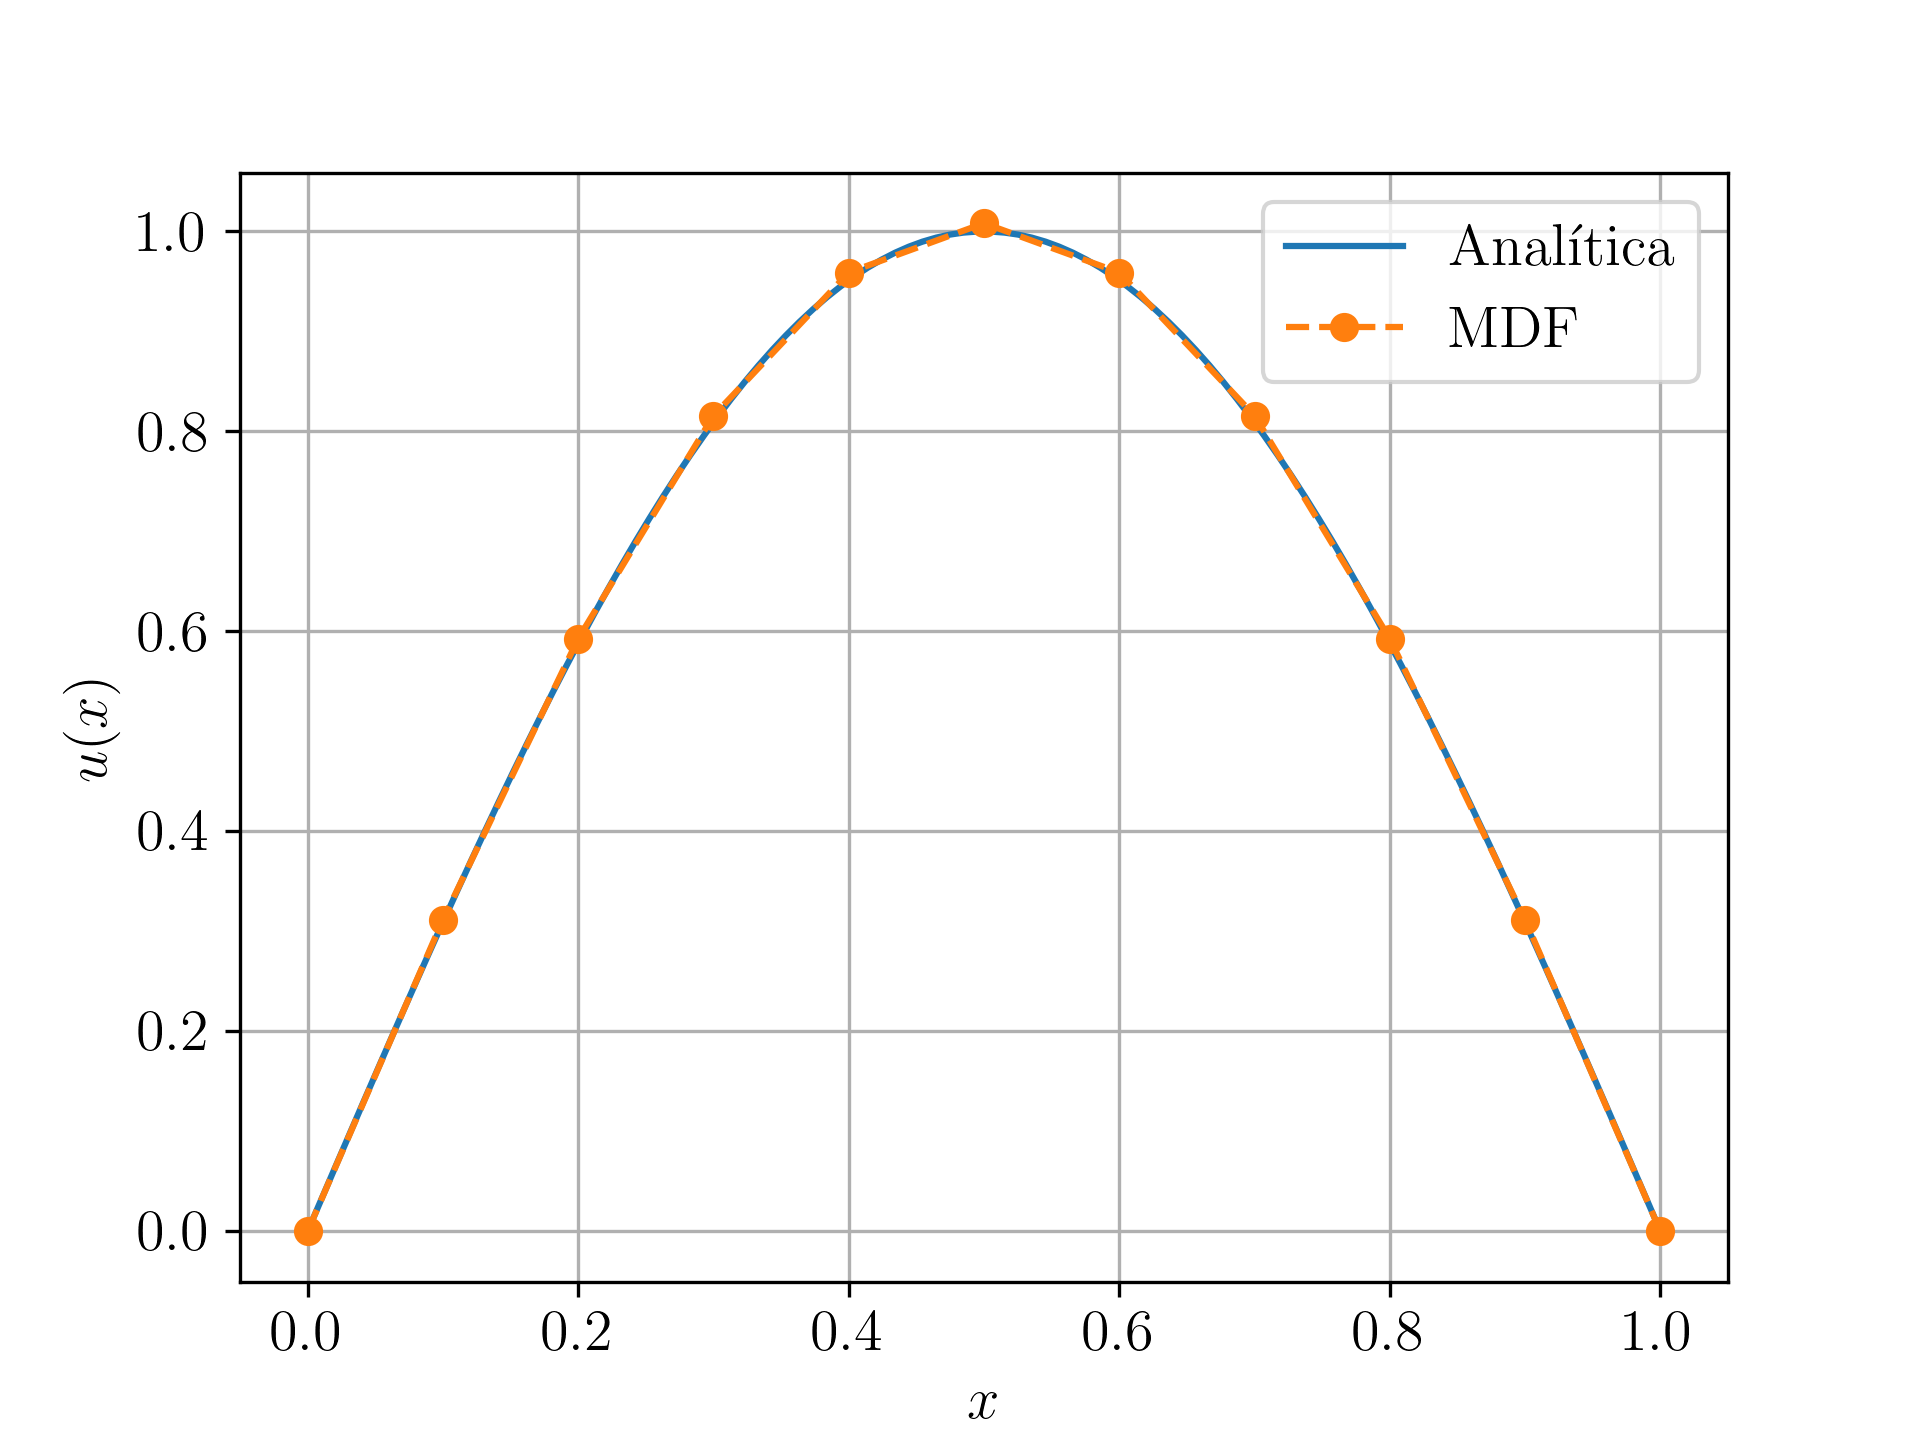
\includegraphics[width=0.8\textwidth]{./cap_pvc/dados/fig_mdf/fig}
  \caption{Resultado referente ao Exemplo~\ref{cap_pvc_sec_mdf:ex:pvc_mdf_1}.}
  \label{cap_pvc_sec_mdf:fig:ex_pvc_mdf_1}
\end{figure}

A solução analítica deste problema é $u(x) = \sen(\pi x)$. Usando o MDF como acima, encontramos o problema discreto
\begin{subequations}
  \begin{align}
    u_1 &= 0,\\
    -\frac{1}{h^2}u_{i-1} + \frac{2}{h^2}u_i - \frac{1}{h^2}u_{i+1} &= \pi^2\sen(\pi x_i),\\
    u_{n+1} &= 0,
  \end{align}
\end{subequations}
com tamanho de malha $h=1/n$ e nodos $x_i = (i-1)h$ indexados por $i = 1, 2, \dotsc, n+1$.

\begin{table}[h!]
  \centering
  \caption{Resultados referentes ao Exemplo~\ref{cap_pvc_sec_mdf:ex:pvc_mdf_1}.}
  \begin{tabular}{l|c}\toprule
    $h$ & $\|\tilde{u} - u\|_{L^2}$ \\\midrule
    $1.0\e-1$ & $1.8\e-2$\\
    $5.0\e-2$ & $6.5\e-3$\\
    $2.5\e-2$ & $2.3\e-3$\\
    $1.0\e-3$ & $5.8\e-4$\\\bottomrule
  \end{tabular}
  \label{cap_pvc_sec_mdf:tab:ex_pvc_mdf_1}
\end{table}

Resolvendo este sistema com $h=10^{-1}$ obtemos a solução numérica apresentada na Figura~\ref{cap_pvc_sec_mdf:fig:ex_pvc_mdf_1}. Ainda, na Tabela~\ref{cap_pvc_sec_mdf:tab:ex_pvc_mdf_1} temos a comparação na norma $L^2$ da solução numérica $\tilde{\pmb{u}}$ com a solução analítica $\pmb{u} = (u(x_i))_{i=1}^{n+1}$ para diferentes escolhas de $h$.

\begin{lstlisting}[caption=pvc\_mdf.py]
import numpy as np

# malha
n = 10
h = 1./n
xx = np.linspace(0., 1., n+1)

# fonte
def f(x):
    return np.pi**2*np.sin(np.pi*x)

# prob discreto
A = np.zeros((n+1, n+1))
b = np.empty(n+1)

# c.c. x = 0.
A[0,0] = 1.
b[0] = 0.

# pts internos
for i in range(1,n):
    A[i,i-1] = -1./h**2
    A[i,i] = 2./h**2
    A[i,i+1] = -1./h**2
    b[i] = f(xx[i])

# c.c. x = 1.
A[n,n] = 1.
b[n] = 0.

# resol
u = npla.solve(A, b)
\end{lstlisting}
\end{ex}

\subsection{Exercícios}

\begin{exer}
  Considere o PVC
  \begin{align}
    &-u'' = \pi^2\cos(\pi x), ~0 < x < 1,\\
    &u(0) = 1,\\
    &u(1) = -1.
  \end{align}
  A solução analítica deste problema é $u(x) = \cos(\pi x)$. Use o MDF para computar aproximações numéricas $\tilde{\pmb{u}}_h$ com tamanhos de malha $h=10^{-1}, 10^{-2}, 10^{-3}, 10^{-4}$ e verifique o erro absoluto $\varepsilon_{\text{abs}} := \|\tilde{\pmb{u}}_h - \pmb{u}\|$.
\end{exer}
\begin{resp}
  \begin{tabular}{l|c}\toprule
    $h$ & $\|\tilde{u} - u\|_{L^2}$ \\\midrule
    $10^{-1}$ & $3.9\e-3$\\
    $10^{-2}$ & $1.2\e-4$\\
    $10^{-3}$ & $3.9\e-6$\\
    $10^{-4}$ & $1.2\e-7$\\\bottomrule
  \end{tabular}  
\end{resp}

\begin{exer}
  Considere o PVC
  \begin{align}
    &-u'' = 1, ~-1 < x < 1,\\
    &u(-1) = 0,\\
    &u(1) = 0.
  \end{align}
  A solução analítica deste problema é $u(x) = 1-x^2$. Use o MDF com $n=20$ subintervalos na malha e verifique o erro absoluto $\varepsilon_{\text{abs}} := \|\tilde{\pmb{u}}_h - \pmb{u}\|$. Por que o erro está próximo precisão de máquina? Justifique sua resposta.
\end{exer}
\begin{resp}
  $\varepsilon_{\text{abs}} = 3.1\e-14$.
\end{resp}

\begin{exer}
Considere o seguinte PVC
\begin{subequations}
  \begin{align}
    &-u'' + u' = f(x), ~-1 < x < 1,\\
    &u(-1) = 0,\\
    &u'(1) =0,
  \end{align}
\end{subequations}
onde
\begin{equation}
  f(x) = \left\{
    \begin{array}{ll}
      1 &, x\leq 0\\
      0 &, x>0
    \end{array}
  \right.
\end{equation}
Use uma aproximação adequada pelo método de diferenças finitas para obter o valor aproximado de $u(0)$ com precisão de $2$ dígitos significativos.
\end{exer}
\begin{resp}
  $7,2\E-1$
\end{resp}

\begin{exer}
  Considere o PVC
  \begin{align}
    &-u'' = \pi^2\cos(\pi x), ~0 < x < 1,\\
    &u(0) = 1,\\
    &u'(1) = 0.
  \end{align}
  A solução analítica deste problema é $u(x) = \cos(\pi x)$. Aplique o MDF para computar aproximações numéricas usando a:
  \begin{enumerate}[a)]
  \item fórmula de diferenças finitas $D_{-,h}u(x)$ no contorno $x=1$.
  \item fórmula de diferenças finitas $D_{-,h^2}u(x)$ no contorno $x=1$.
  \end{enumerate}
  Quais das duas produz o resultado mais preciso? Justifique sua resposta.
\end{exer}
\begin{resp}
  b) resultado mais preciso.
\end{resp}

\section{Método de Elementos Finitos}\label{cap_pvc_sec_fem}

Consideramos o seguinte problema linear de valor de contorno (PVC)
\begin{subequations}\label{cap_pvc_sec_fem:eq:pvc}\hleq
  \begin{align}
    &-u'' = f(x), ~a < x < b, \label{cap_pvc_sec_fem:eq:pvc_eq}\\
    &u(a) = 0, \label{cap_pvc_sec_fem:eq:pvc_bc1}\\
    &u(b) = 0. \label{cap_pvc_sec_fem:eq:pvc_bc2}
  \end{align}
\end{subequations}
onde a incógnita é $u = u(x)$ com dada fonte $f = f(x)$.

\hl{A solução pelo \emph{Método de Elementos Finitos} (FEM) de {\eqref{cap_pvc_sec_mdf:eq:pvc_eq}}-{\eqref{cap_pvc_sec_mdf:eq:pvc_bc2}} surge da aproximação do problema em um espaço de dimensão finita de funções}. São três passos fundamentais: 1. escrever a formulação fraca do problema\footnote{Por convenção, {\eqref{cap_pvc_sec_mdf:eq:pvc_eq}}-{\eqref{cap_pvc_sec_mdf:eq:pvc_bc2}} é chamado de formulação forte do problema.}, 2. escrever a formulação de elementos finitos e 3. resolver o problema de elementos finitos.

\begin{flushleft}
  \textbf{1. Formulação Fraca}
\end{flushleft}

Para obter a \emph{formulação fraca} do PVC {\eqref{cap_pvc_sec_fem:eq:pvc_eq}}-{\eqref{cap_pvc_sec_fem:eq:pvc_bc2}}, multiplicamos \eqref{cap_pvc_sec_fem:eq:pvc_eq} por uma arbitrária função teste $v = v(x)$
\begin{equation}
  -u''v = fv
\end{equation}
e integramos no domínio $a \leq x \leq b$, i.e.
\begin{equation}
    -\int_a^bu''v\,dx = \int_a^bfv\,dx.
\end{equation}
Então, aplicando \emph{integração por partes} no primeiro termo do lado esquerdo, obtemos
\begin{equation}
    \int_a^bu'v'\,dx - \left[u'v\right]_{x=a}^b = \int_a^bfv\,dx.
\end{equation}

Vamos denotar o produto interno em $L^2([a,b])$\footnote{$u\in L^2([a,b]) \Leftrightarrow \int_a^b |u|^2\,dx < \infty$.} por
\begin{equation}
  (u, v)_2 := \int_a^b uv\,dx
\end{equation}
e nos contornos
\begin{equation}
  \langle u, v \rangle := u(b)v(b) - u(a)v(a).
\end{equation}
Com isso, definimos a \hlemph{formulação fraca} como o seguinte problema: \hl{encontrar $u\in V := H_0^1([a,b])$\footnote{$H_0^1([a,b]) := \{u=u(x);~u,u'\in L^2([a,b]), u(a)=u(b)=0\}$.} tal que}
\begin{equation}\hleq\label{cap_pvc_sec_fem:eq:prob_fraco}
  a(u, v) = l(v), ~\forall v\in V,
\end{equation}
onde a \emph{forma bilinear} é
\begin{equation}
  a(u, v) := (u', v')_2
\end{equation}
e a \emph{forma linear} é
\begin{equation}
  l(v) := (f, v)_2.
\end{equation}

\begin{flushleft}
  \textbf{2. Formulação de Elementos Finitos}
\end{flushleft}

\hl{A \emph{formulação de elementos finitos} do problema {\eqref{cap_pvc_sec_fem:eq:pvc_eq}}-{\eqref{cap_pvc_sec_fem:eq:pvc_bc2}} é obtida a partir de {\eqref{cap_pvc_sec_fem:eq:prob_fraco}} pela substituição do espaço de funções $V$ por um \emph{espaço de dimensão finita} $V_h$}. A ideia é que $V_h\to V$, bem como a solução de elementos finitos $u_h\to u\in V$ quando $h\to 0$.

Para construir o \emph{espaço de elementos finitos} $V_h$, vamos considerar elementos do tipo
\begin{equation}
  \begin{aligned}
    P_1(I) := &\left\{v=v(x); v(x)=c_0+c_1x,\right. \\
    &\qquad\qquad\qquad\left. x\in I, c_0,c_1\in\mathbb{R}\right\},
  \end{aligned}
\end{equation}
onde $I$ é um intervalo fechado.

Sobre o domínio, assumimos uma malha uniforme
\begin{equation}
  M([a,b]) := \{x_1, x_2, \dotsc, x_{n+1}\}
\end{equation}
com $h = (b-a)/n$, $x_i = a + (i-1)h$, $i=1, 2, \dotsc, n+1$. Nesta, definimos o espaço de funções
\begin{equation}
  \begin{aligned}
    V_{h,0} &:= \left\{v=v(x); v\in C^0[a,b], v(a)=v(b)=0, \right.\\
    &\left.\qquad\qquad\qquad v|_{[x_i,x_{i+1}]}\in P_1([x_i,x_{i+1}]), i=1, 2, \dotsc, n\right\}.
  \end{aligned}
\end{equation}
Pode-se mostrar que $V_h = \spn\{\phi_i\}_{i=1}^{n-1}$, com base nodal
\begin{equation}
  \phi_j(x_i) = \left\{
    \begin{array}{ll}
      1 &, i=j,\\
      0 &, i\neq j
    \end{array}
\right.
\end{equation}
para $i,j = 2, \dotsc, n$ e $\phi_1(a)=0=\phi_n(b)$. Podemos verificar que
\begin{equation}
  \phi_i(x) = \left\{
    \begin{array}{ll}
      (x-x_{i-1})/h &, x\in [x_{i-1}, x_i],\\
      (x_{i+1}-x)/h &, x\in [x_i, x_{i+1}],\\
      0 &, \text{noutros casos}
    \end{array}
\right.
\end{equation}

Com isso, definimos a \hlemph{formulação de elementos finitos} sendo o seguinte problema: \hl{encontrar $u_h\in V_{h,0}$ tal que}
\begin{equation}
  a(u_h, v_h) = l(v_h), ~\forall v_h\in V_h.
\end{equation}
Tendo em vista que $V_h = \spn\{\phi_i\}_{i=1}^{n+1}$, este é equivalente a
\begin{equation}\label{cap_pvc_sec_mef:eq:fef}\hleq
  a(u_h, \phi_j) = l(\phi_j), ~\forall 1\leq j \leq n-1.
\end{equation}

\begin{flushleft}
  \textbf{3. Resolução do Problema de Elementos Finitos}
\end{flushleft}

\hl{O problema de elementos finitos {\eqref{cap_pvc_sec_mef:eq:fef}} consiste em um sistema linear} $\hleq A\pmb{u} = \pmb{b}$. De fato, a solução $u_h\in V_{h,0}$ pode ser escrita como a seguinte combinação linear
\begin{equation}
  u_h = \sum_{j=1}^{n-1}u_j\phi_j.
\end{equation}
Logo, temos que
\begin{subequations}
  \begin{align}
    a(u_h, \phi_i) &= \left(\sum_{j=1}^{n-1}u_j\phi_j, \phi_i\right)_2,\\
                   &= \sum_{j=1}^{n-1}u_j(\phi_j,\phi_i)_2,\\
                   &= A\pmb{u},
  \end{align}
\end{subequations}
onde a \hlemph{matriz dos coeficientes} é $\hleq{A = \left[a_{i,j}:=(\phi_j, \phi_i)\right]_{i,j=1}^{n-1}}$ e o \hlemph{vetor das incógnitas} é $\hleq{\pmb{u} = (u_j)_{j=1}^{n-1}}$. Doutro lado, temos
\begin{equation}
  l(\phi_i) = (f, \phi_i)_2,
\end{equation}
o que nos fornece o \hlemph{vetor dos termos constantes} $\hleq \pmb{b} = \left(b_i:=(f, \phi_i)_2\right)_{i=1}^{n-1}$.

O cálculo dos elementos de $A$ fornece
\begin{subequations}
  \begin{align}
    a_{i,i} &= (\phi'_i, \phi'_i)_2\\
            &= \int_a^b \left(\phi'_i\right)^2\,dx\\
            &= \int_{x_{i-1}}^{x_{i+1}}(\phi'_i)^2\,dx\\
            &= \int_{x_{i-1}}^{x_{i}} \left[\left(\frac{x-x_{i-1}}{h}\right)'\right]^2\,dx\\
            &+ \int_{x_{i}}^{x_{i+1}} \left[\left(\frac{x_{i+1}-x}{h}\right)'\right]^2\,dx\\
            &= \frac{2}{h}, ~i=1, 2, \dotsc, n-1,
  \end{align}
\end{subequations}
\begin{subequations}
  \begin{align}
    a_{i,i+1} &= (\phi'_{i+1}, \phi'_i)_2\\
            &= \int_a^b \phi'_{i+1}\phi'_i\,dx\\
            &= \int_{x_i}^{x_{i+1}}\left(\frac{x_{i+1}-x}{h}\right)'\left(\frac{x - x_{i+1}}{h}\right)'\,dx\\
            &= -\frac{1}{h}, ~i=1, 2, \dotsc, n-2,
  \end{align}
\end{subequations}
\begin{subequations}
  \begin{align}
    a_{i-1,i} &= (\phi'_{i-1}, \phi'_i)_2\\
            &= \int_a^b \phi_{i-1}\phi_i\,dx\\
            &= \int_{x_{i-1}}^{x_{i}}\left(\frac{x_i-x}{h}\right)'\left(\frac{x - x_{i}}{h}\right)'\,dx\\
            &= -\frac{1}{h}, ~i=2, \dotsc, n-1,
  \end{align}
\end{subequations}
observando que, noutros casos, $a_{i,j} = 0$.

Um cálculo aproximado dos elementos de $\pmb{b}$ fornece\footnote{Por simplicidade, usando a regra do ponto médio para aproximar as integrais.}
\begin{subequations}
  \begin{align}
    b_i &= (f, \phi_i)_2\\
        &= \int_a^b f(x)\phi_i(x)\,dx\\
        &= \int_{x_{i-1}}^{x_{i}} f(x)\frac{(x-x_{i-1})}{h}\,dx\\
        &+ \int_{x_{i}}^{x_{i+1}} f(x)\frac{(x_{i+1}-x)}{h}\,dx\\
        &\approx \frac{h}{2}f(x_{i-1/2}) + \frac{h}{2}f(x_{i+1/2}).
  \end{align}
\end{subequations}

\begin{ex}\label{cap_pvc_sec_mef:ex:pvc_mef}
  Consideramos o seguinte PVC
  \begin{align}
    &-u'' = \pi^2\sen(\pi x), ~0 < x < 1,\\
    &u(0) = 0,\\
    &u(1) = 0.
  \end{align}
  A solução analítica deste problema é $u(x) = \sen(\pi x)$.
  
  \begin{figure}[h!]
    \centering
    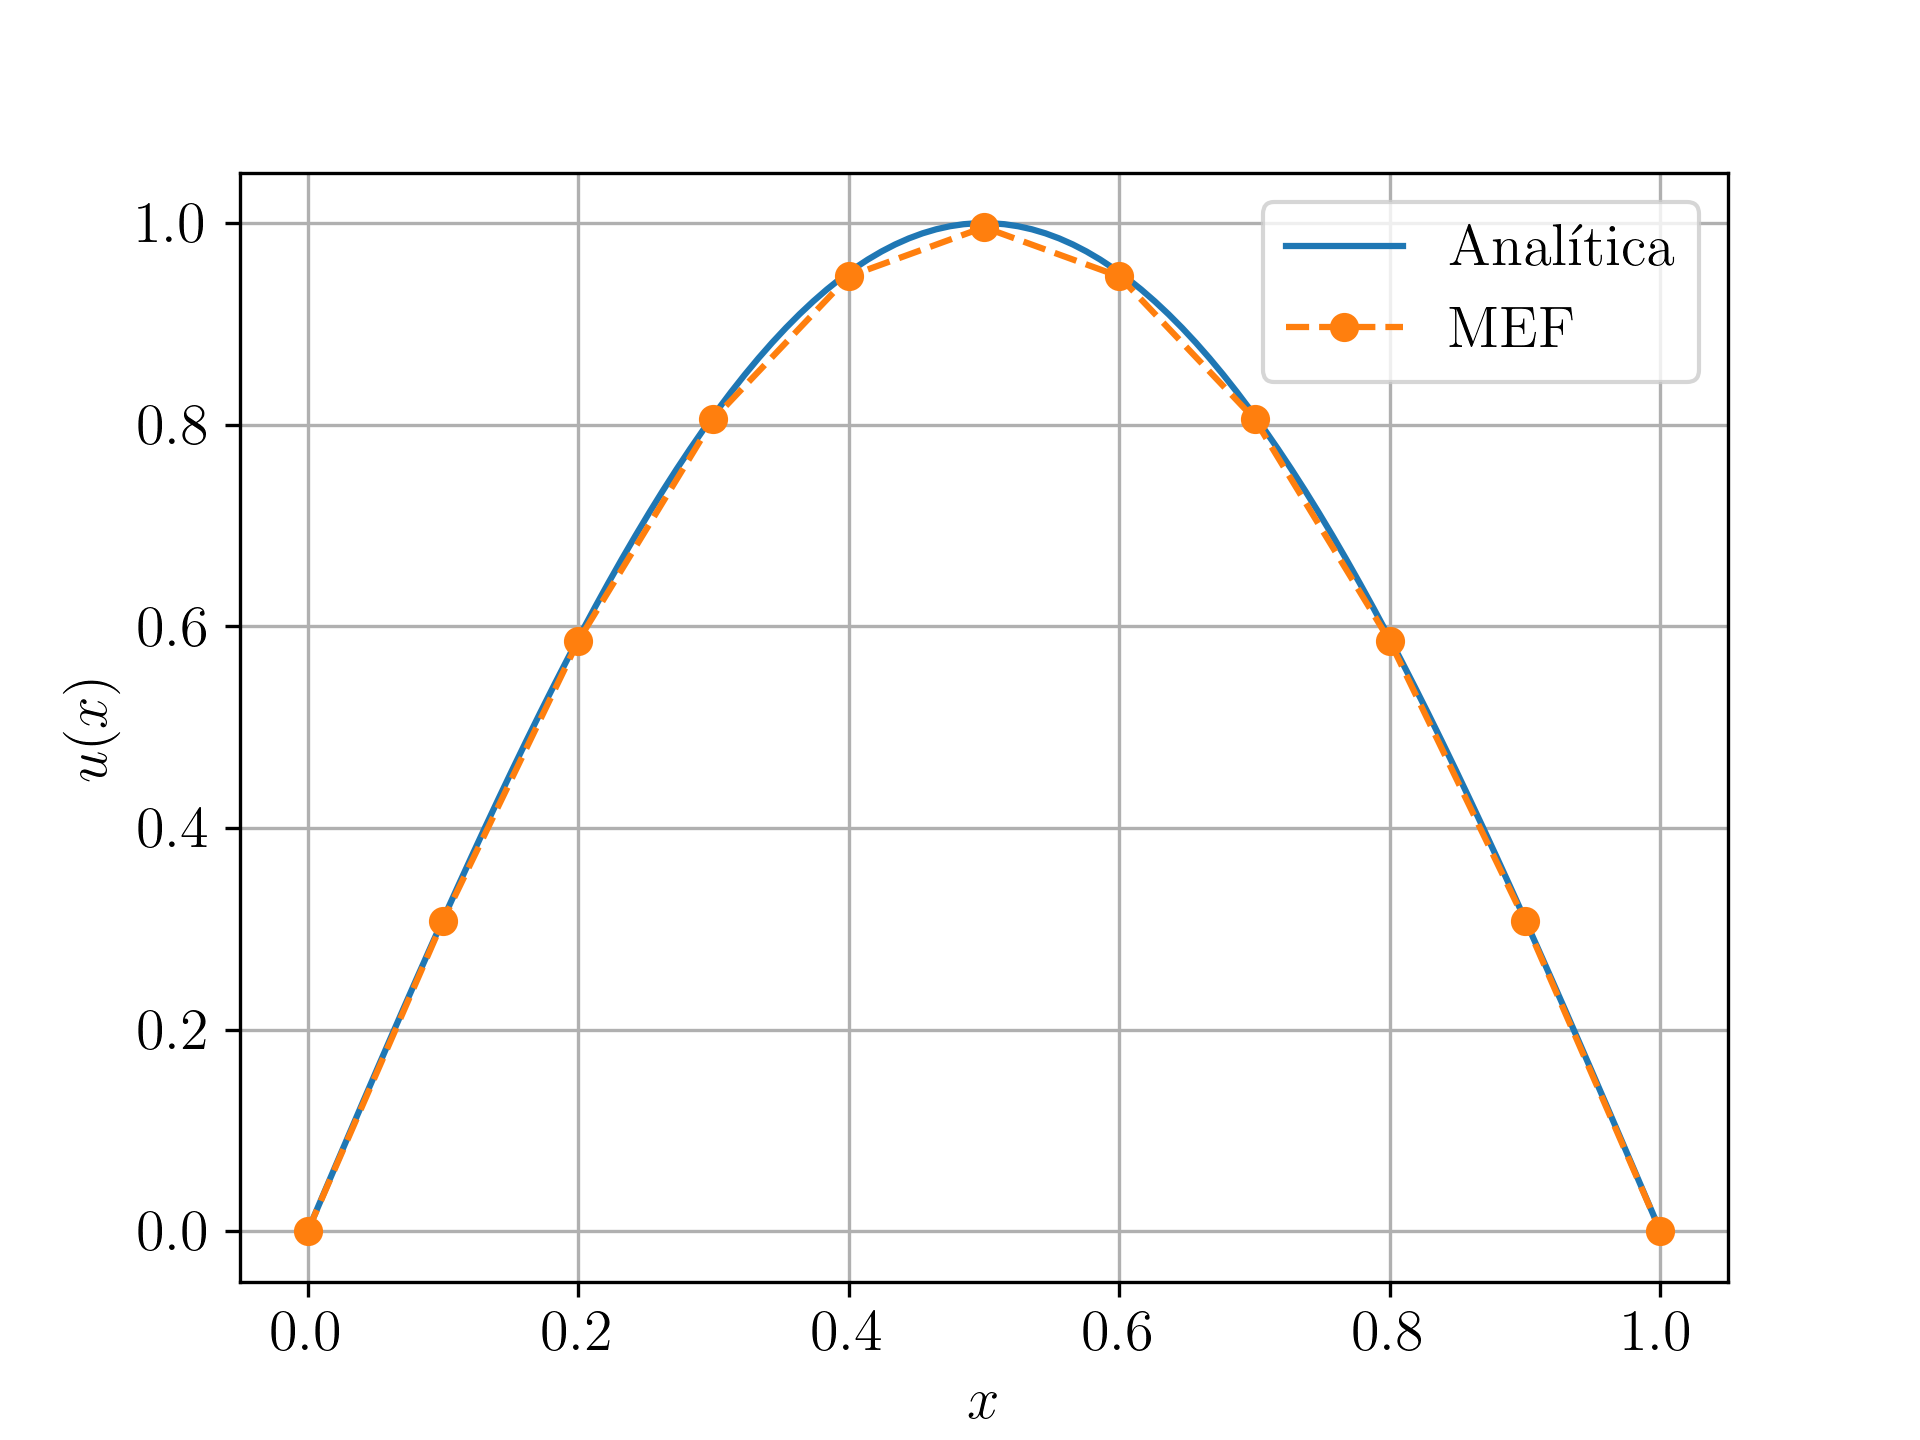
\includegraphics[width=0.8\textwidth]{./cap_pvc/dados/fig_mef/fig}
    \caption{Resultado referente ao Exemplo~\ref{cap_pvc_sec_mef:ex:pvc_mef}.}
    \label{cap_pvc_sec_mef:fig:ex_pvc_mef}
  \end{figure}

Resolvendo este sistema com $h=10^{-1}$ obtemos a solução numérica apresentada na Figura~\ref{cap_pvc_sec_mef:fig:ex_pvc_mef}.

\begin{lstlisting}[caption=pvc\_mef.py]
import numpy as np

# malha
n = 10
h = 1./n
xx = np.linspace(0., 1., n+1)

# fonte
def f(x):
    return np.pi**2*np.sin(np.pi*x)

# prob discreto
A = np.zeros((n-1, n-1))
b = np.empty(n-1)

# c.c. x = 0.
A[0,0] = 2./h
A[0,1] = -1./h
b[0] = h/2 * (f(xx[1]-0.5*h) + f(xx[1]+0.5*h))

# pts internos
for i in range(1,n-2):
    A[i,i-1] = -1./h
    A[i,i] = 2./h
    A[i,i+1] = -1./h
    b[i] = h/2 * (f(xx[i+1]-0.5*h) + f(xx[i+1]+0.5*h))

# c.c. x = 1.
A[n-2,n-3] = -1./h
A[n-2,n-2] = 2./h
b[n-2] = h/2 * (f(xx[n-1]-0.5*h) + f(xx[n-1]+0.5*h))

# resol
u = npla.solve(A, b)
## c.c. (dirichlet)
u = np.concatenate(([0.],u,[0.]))
\end{lstlisting}
\end{ex}

\subsection{Exercícios}

\begin{exer}
  Considere o PVC
  \begin{align}
    &-u'' = \pi^2\cos(\pi x), ~0 < x < 1,\\
    &u(0) = 1,\\
    &u(1) = -1.
  \end{align}
  A solução analítica deste problema é $u(x) = \cos(\pi x)$. Use o MEF para computar aproximações numéricas $\tilde{\pmb{u}}_h$ com tamanhos de malha $h=10^{-1}, 10^{-2}, 10^{-3}, 10^{-4}$ e verifique o erro absoluto $\varepsilon_{\text{abs}} := \|\tilde{\pmb{u}}_h - \pmb{u}\|$.
\end{exer}

\begin{exer}
  Considere o PVC
  \begin{align}
    &-u'' = 1, ~-1 < x < 1,\\
    &u(-1) = 0,\\
    &u(1) = 0.
  \end{align}
  A solução analítica deste problema é $u(x) = 1-x^2$. Use o MEF com $n=20$ subintervalos na malha e verifique o erro absoluto $\varepsilon_{\text{abs}} := \|\tilde{\pmb{u}}_h - \pmb{u}\|$. Por que o erro está próximo precisão de máquina? Justifique sua resposta.
\end{exer}

\begin{exer}
Considere o seguinte PVC
\begin{subequations}
  \begin{align}
    &-u'' + u' = f(x), ~-1 < x < 1,\\
    &u(-1) = 0,\\
    &u'(1) =0,
  \end{align}
\end{subequations}
onde
\begin{equation}
  f(x) = \left\{
    \begin{array}{ll}
      1 &, x\leq 0\\
      0 &, x>0
    \end{array}
  \right.
\end{equation}
Use uma aproximação adequada pelo MEF para obter o valor aproximado de $u(0)$ com precisão de $2$ dígitos significativos.
\end{exer}
\begin{resp}
  $7,2\E-1$
\end{resp}

\begin{exer}
  Considere o PVC
  \begin{align}
    &-u'' = \pi^2\cos(\pi x), ~0 < x < 1,\\
    &u(0) = 1,\\
    &u'(1) = 0.
  \end{align}
  A solução analítica deste problema é $u(x) = \cos(\pi x)$. Aplique o MEF para computar uma aproximação numérica com erro absoluto de no máximo $10^{-3}$ na norma $L^2$.
\end{exer}

\section{Método de Volumes Finitos}\label{cap_pvc_sec_mvf}

\hl{O \emph{Método de Volumes Finitos} (MVF) é um método de discretização apropriado para problemas conservativos}. Consideramos o seguinte problema linear de valor de contorno (PVC)
\begin{subequations}\label{cap_pvc_sec_mvf:eq:pvc}\hleq
  \begin{align}
    &-u_{xx} = f(x), ~a < x < b, \label{cap_pvc_sec_mvf:eq:pvc_eq}\\
    &u(a) = 0, \label{cap_pvc_sec_mvf:eq:pvc_bc1}\\
    &u(b) = 0. \label{cap_pvc_sec_mvf:eq:pvc_bc2}
  \end{align}
\end{subequations}
onde a incógnita é $u = u(x)$ com dada fonte $f = f(x)$. A Eq.~\eqref{cap_pvc_sec_mvf:eq:pvc} pode ser reescrita na forma conservativa
\begin{equation}
  \ddiv(\pmb{F}) = f,
\end{equation}
onde $\pmb{F} = -u_x$

\begin{flushleft}
  \hlemph{1. Discretização Espacial.}
\end{flushleft}

Assumimos uma malha do domínio $[a, b]$ da forma
\begin{equation}
  a = x_{\frac{1}{2}} < x_1 < x_{\frac{3}{2}} < \cdots < x_{i-\frac{1}{2}} < x_i < x_{i+\frac{1}{2}} < \cdots < x_{n} < x_{n+\frac{1}{2}} = b,
\end{equation}
onde $h = (b-a)/n$, $x_{i-\frac{1}{2}} = a + (i-1)h$, $h^{-} = h^{+} = h/2$, $i = 1, 2, \dotsc, n$. Também denotamos $K_i = \left(x_{i-\frac{1}{2}}, x_{i+\frac{1}{2}}\right)$ a $i$-ésima célula da malha.

\begin{flushleft}
  \hlemph{2. Discretização das Equações.}
\end{flushleft}

No MVF, as incógnitas $u_i$, $i = 1, 2, \dotsc, n$, são as aproximações para o valor médio de $u$ nas células $K_i$, i.e.
\begin{equation}
  u_i = \frac{1}{|K_i|}\int_{a}^{b}u(x)\,dx.
\end{equation}
O sistema discreto para $u_i$ é obtido tomando a média da Eq.~\label{cap_pvc_sec_fem:eq:pvc_eq} na célula $K_i$, donde temos
\begin{subequations}
  \begin{align}
    &-\frac{1}{h}\int_{x_{i-\frac{1}{2}}}^{x_{i+\frac{1}{2}}}u_{xx}\,dx = \frac{1}{h}\int_{K_i}f\,dx,\\
    &\hleq \frac{1}{h}\left[-u_x\left(x_{i+\frac{1}{2}}\right) + u_x\left(x_{i-\frac{1}{2}}\right)\right] = \frac{1}{h}\int_{K_i}f\,dx\label{cap_pvc_sec_mvf:eq:aux00}
  \end{align}
\end{subequations}
Por fórmula de diferenças finitas central, temos
\begin{equation}
  u_{x}\left(x_{i+\frac{1}{2}}\right) = \frac{u_i - u_{i-1}}{h} + O(h)
\end{equation}
e
\begin{equation}
  u_x\left(x_{i-\frac{1}{2}}\right) = \frac{u_{i+1} - u_i}{h} + O(h)
\end{equation}
Com isso, obtemos as equações
\begin{equation}\label{cap_pvc_sec_mvf:eq:aux0}
  \frac{1}{h}\left(-\frac{u_{i+1}-u_{i}}{h} + \frac{u_i - u_{i-1}}{h}\right) = \frac{1}{h}\int_{K_i}f\,dx,
\end{equation}
Rearranjando os termos e aproximando a integral de $f$ pela \href{https://notaspedrok.com.br/notas/MatematicaNumericaII/cap_integr_sec_nc.html}{\emph{regra do ponto médio}}, obtemos
\begin{equation}\label{cap_pvc_sec_mvf:eq:aux}
  -\frac{1}{h^2}u_{i-1} + \frac{2}{h^2}u_i - \frac{1}{h^2}u_{i+1} = f_i,
\end{equation}
onde $f_i := f(x_i)$ e $i = 2, 3, \dotsc, n-1$.

Na célula $K_1$, tomamos a aproximação
\begin{subequations}
  \begin{align}
    u_x\left(x_{\frac{1}{2}}\right) &= \frac{u_{1} - u_{\frac{1}{2}}}{h/2} + O\left(h\right),\\
                                    &= = \frac{u_{1}}{h/2} + O\left(h\right).
  \end{align}
\end{subequations}
Aplicando na Eq.~\eqref{cap_pvc_sec_mvf:eq:aux00}, obtemos
\begin{equation}\hleq
  \frac{1}{h}\left(-\frac{u_{2}-u_{1}}{h} + \frac{u_1}{h/2}\right) = \frac{1}{h}\int_{K_i}f\,dx,
\end{equation}
Analogamente, integrando na célula $K_n$ de fronteira, obtemos
\begin{equation}\hleq
  \frac{1}{h}\left(\frac{u_{n}}{h/2} + \frac{u_{n} - u_{n-1}}{h}\right) = \frac{1}{h}\int_{K_i}f\,dx.
\end{equation}

Por fim, obtemos o \hlemph{sistema discreto}
\begin{subequations}\hleq
  \begin{align}
    &\frac{3}{h^2}u_1 - \frac{1}{h^2}u_{2} = f_1,\\
    &-\frac{1}{h^2}u_{i-1} + \frac{2}{h^2}u_i - \frac{1}{h^2}u_{i+1} = f_i,\\
    &-\frac{1}{h^2}u_{n-1} + \frac{3}{h^2}u_{n+1} = f_n,
  \end{align}
\end{subequations}
para $i = 2, 3, \dotsc, n-1$.

\begin{ex}\label{cap_pvc_sec_mvf:ex:pvc_mvf}
  Consideramos o seguinte PVC
  \begin{align}
    &-u'' = \pi^2\sen(\pi x), ~0 < x < 1,\\
    &u(0) = 0,\\
    &u(1) = 0.
  \end{align}
  A solução analítica deste problema é $u(x) = \sen(\pi x)$.
  
  \begin{figure}[h!]
    \centering
    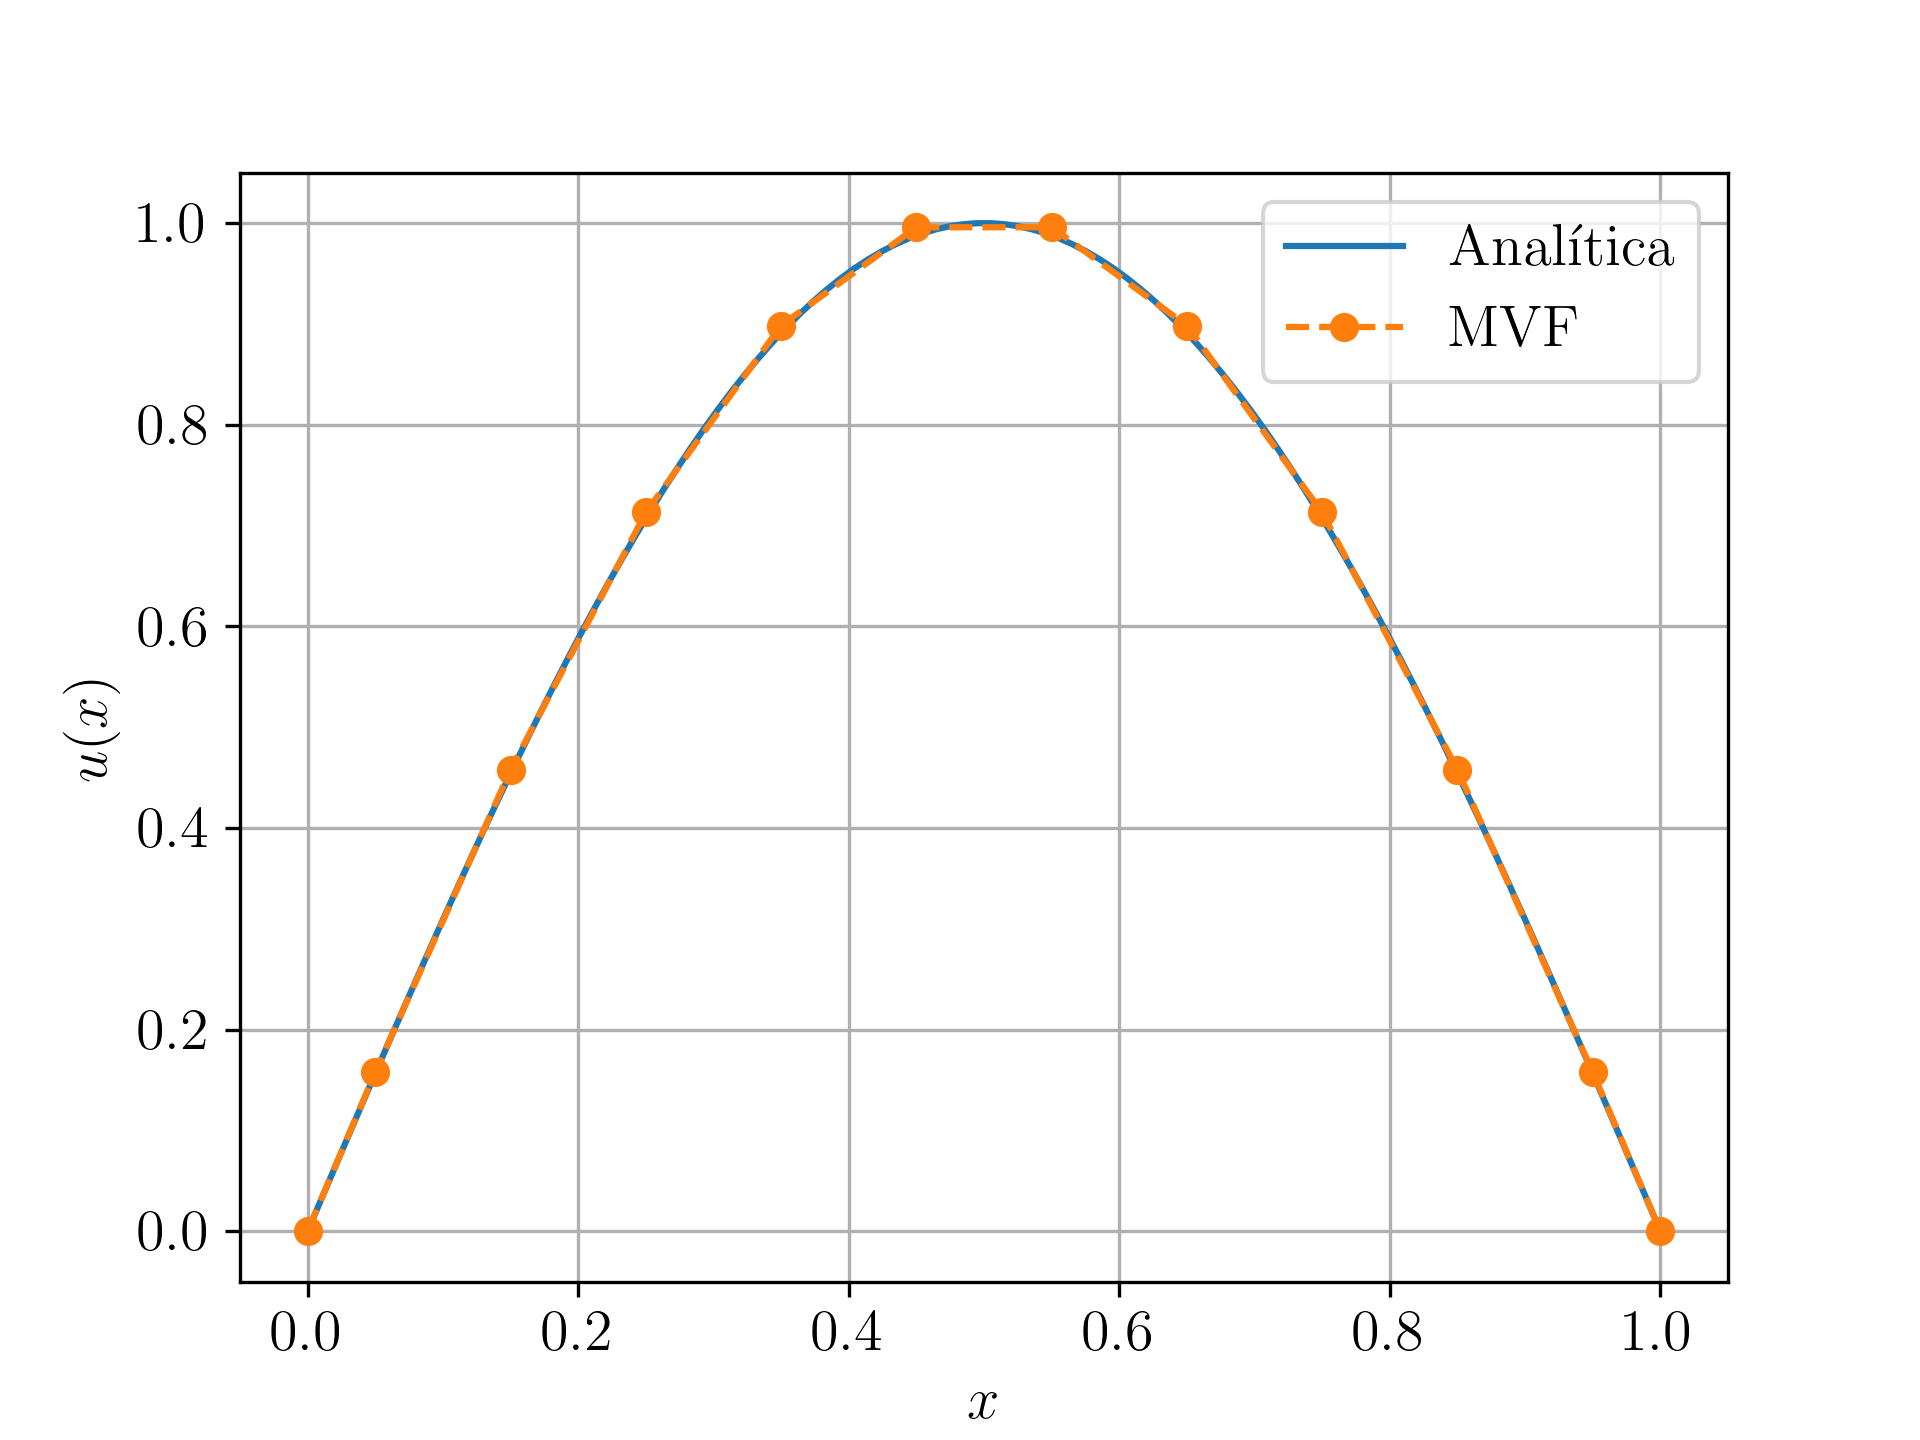
\includegraphics[width=0.8\textwidth]{./cap_pvc/dados/fig_mvf/fig}
    \caption{Resultado referente ao Exemplo~\ref{cap_pvc_sec_mvf:ex:pvc_mvf}.}
    \label{cap_pvc_sec_mvf:fig:ex_pvc_mvf}
  \end{figure}

  Resolvendo este sistema com $h=10^{-1}$ obtemos a solução numérica apresentada na Figura~\ref{cap_pvc_sec_mvf:fig:ex_pvc_mvf}.

\begin{lstlisting}[caption=pvc\_mvf.py]
import numpy as np

# fonte
def f(x):
  return np.pi**2*np.sin(np.pi*x)

# malha
n = 10
h = 1./n
xx = np.linspace(h/2, 1.-h/2, n)

# prob. discreto
A = np.zeros((n,n))
b = np.empty(n)

# c.c. x = 0
A[0,0] = 3./h**2
A[0,1] = -1./h**2
b[0] = f(xx[0])

# pts internos
for i in range(1,n-1):
  A[i,i-1] = -1./h**2
  A[i,i] = 2./h**2
  A[i,i+1] = -1./h**2
  b[i] = f(xx[i])

# c.c. x = 1
A[n-1,n-2] = -1./h**2
A[n-1,n-1] = 3./h**2
b[n-1] = f(xx[n-1])

# resol prob disc
u = npla.solve(A, b)

xx = np.concatenate(([0.],xx,[1.]))
u = np.concatenate(([0.],u,[0.]))
\end{lstlisting}
\end{ex}

\subsection{Exercícios}

\begin{exer}
  Considere o PVC
  \begin{align}
    &-u'' = \pi^2\cos(\pi x), ~0 < x < 1,\\
    &u(0) = 1,\\
    &u(1) = -1.
  \end{align}
  A solução analítica deste problema é $u(x) = \cos(\pi x)$. Use o MVF para computar aproximações numéricas $\tilde{\pmb{u}}_h$ com tamanhos de malha $h = 10^{-1}$, $10^{-2}$, $10^{-3}$, $10^{-4}$ e verifique o erro absoluto $\varepsilon_{h,\text{abs}} := \|\tilde{\pmb{u}}_h - \pmb{u}\|$.
\end{exer}

\begin{exer}
  Considere o PVC
  \begin{align}
    &-u'' = 1, ~-1 < x < 1,\\
    &u(-1) = 0,\\
    &u(1) = 0.
  \end{align}
  A solução analítica deste problema é $u(x) = 1-x^2$. Use o MVF com $n=20$ subintervalos na malha e verifique o erro absoluto $\varepsilon_{\text{abs}} := \|\tilde{\pmb{u}}_h - \pmb{u}\|$.
\end{exer}

\begin{exer}
Considere o seguinte PVC
\begin{subequations}
  \begin{align}
    &-u'' + u' = f(x), ~-1 < x < 1,\\
    &u(-1) = 0,\\
    &u'(1) =0,
  \end{align}
\end{subequations}
onde
\begin{equation}
  f(x) = \left\{
    \begin{array}{ll}
      1 &, x\leq 0\\
      0 &, x>0
    \end{array}
  \right.
\end{equation}
Use uma aproximação adequada pelo MVF para obter o valor aproximado de $u(0)$ com precisão de $2$ dígitos significativos.
\end{exer}
\begin{resp}
  $7,2\E-1$
\end{resp}

\begin{exer}
  Considere o PVC
  \begin{align}
    &-u'' = \pi^2\cos(\pi x), ~0 < x < 1,\\
    &u(0) = 1,\\
    &u'(1) = 0.
  \end{align}
  A solução analítica deste problema é $u(x) = \cos(\pi x)$. Aplique o MVF para computar uma aproximação numérica com erro absoluto de no máximo $10^{-3}$ na norma $L^2$.
\end{exer}

%Este trabalho está licenciado sob a Licença Atribuição-CompartilhaIgual 4.0 Internacional Creative Commons. Para visualizar uma cópia desta licença, visite http://creativecommons.org/licenses/by-sa/4.0/deed.pt_BR ou mande uma carta para Creative Commons, PO Box 1866, Mountain View, CA 94042, USA.

\chapter{Equações Diferenciais Parciais}\label{cap_edp}
\thispagestyle{fancy}

Neste capítulo, discutimos alguns tópicos fundamentais da aplicação do método de diferenças finitas para a simulação (aproximação da solução) de equações diferenciais parciais.

\section{Equação de Poisson}\label{cap_edp_sec_Poisson}\index{equação! de Poisson}

A equação de Poisson em um domínio retangular $D = (x_{\text{ini}}, x_{\text{fin}})\times (y_{\text{ini}}, y_{\text{fin}})$ com condições de contorno de Dirichlet homogêneas refere-se o seguinte problema
\begin{align}
  u_{xx} + u_{yy} &= f(x, y),~(x, y)\in D, \label{eq:edp_Poisson_eq}\\
  u(x_{\text{ini}}, y) &= 0,~y_{\text{ini}}\leq y \leq y_{\text{fin}},\label{eq:edp_Poisson_bcxini}\\
  u(x_{\text{fin}}, y) &= 0,~y_{\text{ini}}\leq y \leq y_{\text{fin}},\label{eq:edp_Poisson_bcxfin}\\
  u(x, y_{\text{ini}}) &= 0,~x_{\text{ini}}\leq x \leq x_{\text{fin}},\label{eq:edp_Poisson_bcyini}\\
  u(x, y_{\text{fin}}) &= 0,,~x_{\text{ini}}\leq x \leq x_{\text{fin}},\label{eq:edp_Poisson_bcyfin}
\end{align}
onde $u = u(x,y)$ é a incógnita.

A aplicação do método de diferenças finitas para resolver este problema consiste dos mesmos passos usados para resolver problemas de valores de contorno (veja Capítulo~\ref{cap_pvc}), a saber: 1. construção da malha, 2. discretização das equações, 3. resolução do problema discreto.

\begin{flushleft}
  {\bf 1. Construção da malha}
\end{flushleft}

Tratando-se do domínio retangular $\overline{D} = [x_{\text{ini}}, x_{\text{fin}}]\times [y_{\text{ini}}, y_{\text{fin}}]$, podemos construir uma malha do produto cartesiano de partições uniformes dos intervalos $[x_{\text{ini}}, x_{\text{fin}}]$ e $[y_{\text{ini}}, y_{\text{fin}}]$. Mais explicitamente, tomamos
\begin{align}
  x_{i} &:= x_{\text{ini}} + (i-1)h_x,\quad h_x = \frac{x_{\text{fin}}-x_{\text{ini}}}{n_x-1},\\
  y_{j} &:= y_{\text{ini}} + (j-1)h_y,\quad h_y = \frac{y_{\text{fin}}-y_{\text{ini}}}{n_y-1},  
\end{align}
onde $i = 1, 2, \dotsc, n_x$, $j = 1, 2, \dotsc, n_y$, sendo $n_x$ e $n_y$ o número de subintervalos escolhidos para as partições em $x$ e $y$, respectivamente.

O produto cartesiano das partições em $x$ e $y$ nos fornece uma partição do domínio $\overline{D}$ da forma
\begin{equation}
  P(\overline{D}) = \{(x_1, y_1), (x_1, y_2), \dotsc, (x_i, y_j), \dotsc, (x_{n_x}, y_{n_y})\},
\end{equation}
cujos nodos $(x_i, y_j)$ podem ser indexados (enumerados) por $k = j + (i-1)n_x$.  Por simplicidade, no decorrer do texto, assumiremos $n_x=n_y=:n$ e, por conseguinte, $h_x=h_y=h$.

\begin{flushleft}
  {\bf 2. Discretização das equações}
\end{flushleft}

Usando a fórmula de diferenças finitas central de ordem $h^2$ para a segunda derivada, temos
\begin{align}
  u_{xx}(x,y) &= \frac{u(x+h,y)-2u(x,y)+u(x-h,y)}{h^2} + O(h^2),\\
  u_{yy}(x,y) &= \frac{u(x,y+h)-2u(x,y)+u(x,y-h)}{h^2} + O(h^2).
\end{align}
Daí, denotando $u_{ij}\approx u(x_i, y_j)$ temos
\begin{align}
  u_{xx}(x_i,y_j) &= \frac{u_{i+1,j}-2u_{i,j}+u_{i-1,j}}{h^2} + O(h^2),\\
  u_{yy}(x_i,y_j) &= \frac{u_{i,j+1}-2u_{i,j}+u_{i,j-1}}{h^2} + O(h^2).  
\end{align}
Então, da equação~\ref{eq:edp_Poisson_eq} temos
\begin{equation}
  \frac{u_{i+1,j}-2u_{i,j}+u_{i-1,j}}{h^2} + \frac{u_{i,j+1}-2u_{i,j}+u_{i,j-1}}{h^2} + O(h^2) = f(x_i,y_j).
\end{equation}
Adora, denotando $u_k := u_{j+(i-1)n}$, desprezando o termo do erro de truncamento e rearranjando os termos nesta última equação temos
\begin{equation}\label{eq:edp_Poisson_mdf_sis0}
  \frac{1}{h^2}u_{k-n} + \frac{1}{h^2}u_{k-1} -\frac{4}{h^2}u_{k} + \frac{1}{h^2}u_{k+1} + \frac{1}{h^2}u_{k+n} = f(x_i,y_j),
\end{equation}
para $i,j=2, 3, \dotsc, n-1$. Isto é, esta última expressão nos fornece um sistema de $(n-2)^2$ equações para $n^2$ incógnitas $u_k$.

Para fechar o sistema, usamos as condições de contorno \eqref{eq:edp_Poisson_bcxini}-\eqref{eq:edp_Poisson_bcyfin}:
\begin{align}
  u_{1,j} &= 0,\quad u_{n,j}=0,\label{eq:edp_Poisson_mdf_sis1}\\
  u_{i,1} &= 0,\quad u_{i,n}=0\label{eq:edp_Poisson_mdf_sis2},
\end{align}
$i,j=1, 2, \dotsc, n$.

Com isso, o problema discreto obtido da aplicação do método de diferenças finitas consiste no sistema linear de $n^2$ equações \eqref{eq:edp_Poisson_mdf_sis0}-e\eqref{eq:edp_Poisson_mdf_sis2} para as $n^2$ incógnitas $u_k$, $k=1, 2, \dotsc, n^2$.


\begin{flushleft}
  {\bf 3. Resolução do problema discreto}
\end{flushleft}

O problema discreto \eqref{eq:edp_Poisson_mdf_sis0}-\eqref{eq:edp_Poisson_mdf_sis2} pode ser escrito na forma matricial
\begin{equation}
  A\tilde{u} = b,\label{eq:edp_Poisson_prob_disc}
\end{equation}
onde o vetor da incógnitas é $\tilde{u}=(u_1, u_2, \dotsc, u_{n^2})$ e o vetor dos termos contantes $b$ é tal que
\begin{align}
  i=1,n,~j=1, 2, \dotsc, n &:~b_k = 0,\\
  i=1, 2, \dotsc, n,~j=1,n &:~b_k = 0,\\
  i,j=2, 3, \dotsc, n-1 &:~b_k = f(x_i,y_j).
\end{align}
Além disso, a matriz dos coeficientes $A$ é tal que
\begin{align}
  i=1,n,~j=1, 2, \dotsc, n &:~a_{k,k} = 1,\\
  i=1, 2, \dotsc, n,~j=1,n &:~a_{k,k} = 1,\\
  i,j=2, 3, \dotsc, n-1 &:~a(k,k-n)=\frac{1}{h^2},\\
                        &~~a(k,k-1)=\frac{1}{h^2},\\
                        &~~a(k,k)=-\frac{4}{h^2},\\
                        &~~a(k,k+1)=\frac{1}{h^2},\\
                        &~~a(k,k+n)=\frac{1}{h^2}.
\end{align}
Assim sendo, basta empregarmos um método apropriado para resolver o sistema linear \eqref{eq:edp_Poisson_prob_disc} para obter a solução aproximada de $u$ nos nodos $(x_i, y_j)$.


\begin{ex}\label{ex:edp_Poisson}
  Consideremos o seguinte problema
  \begin{align}
    u_{xx} + u_{yy} &= -\sen(x)\sen(y),~(x, y)\in (0, \pi)\times (0, \pi),\\
    u(0, y) &= 0,~y\in [0, \pi],\\
    u(\pi, y) &= 0,~y\in [0, \pi],\\
    u(x, 0) &= 0,~x\in [0, \pi],\\
    u(x, \pi) &= 0,~x\in [0, \pi].
\end{align}


\begin{figure}[h!]
  \centering
  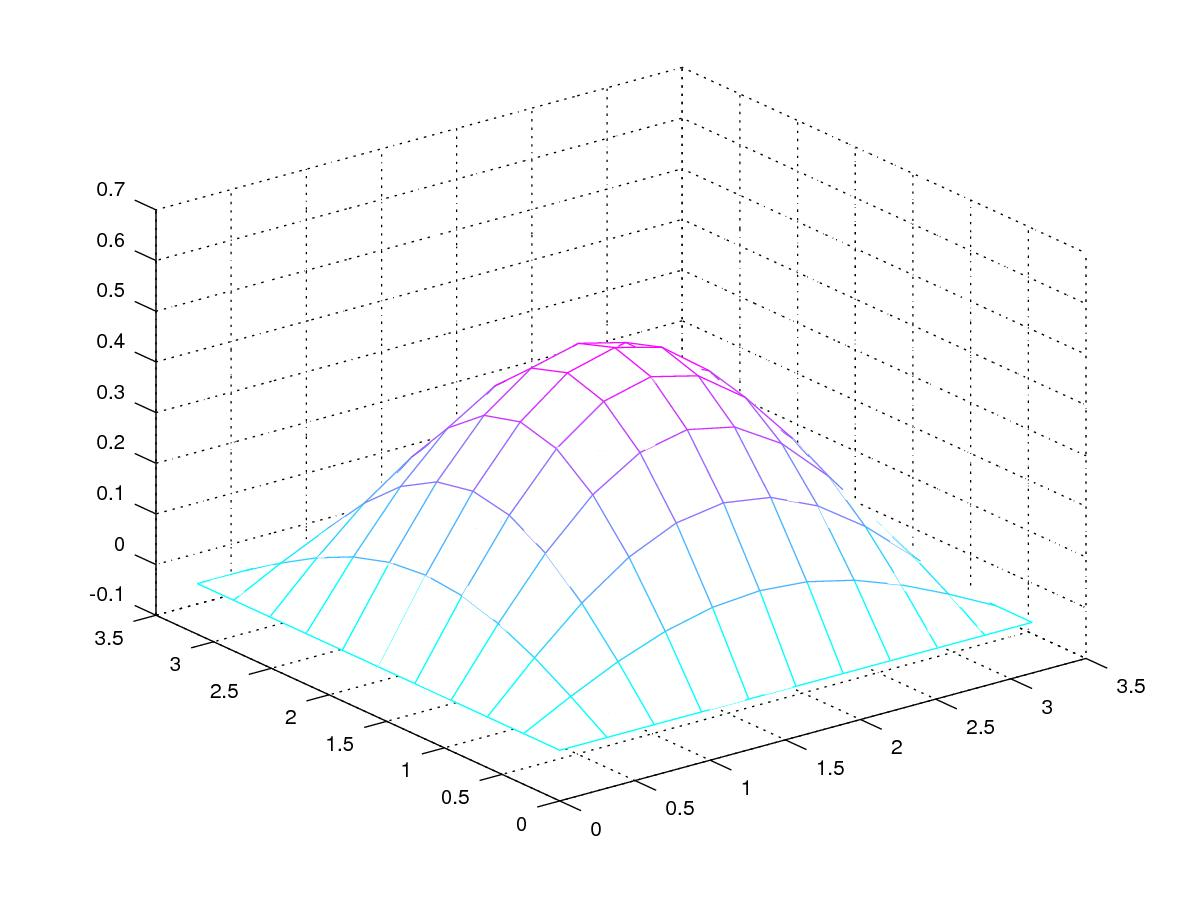
\includegraphics[width=0.8\textwidth]{./cap_edp/dados/ex_edp_Poisson/ex_edp_Poisson}
  \caption{Resultado referente ao Exemplo~\ref{ex:edp_Poisson}.}
  \label{fig:ex_edp_Poisson}
\end{figure}


A Figura~\ref{fig:ex_edp_Poisson} mostra um esboço do gráfico da solução aproximada obtida pelo método de diferenças finitas apresentado acima (equações \eqref{eq:edp_Poisson_mdf_sis0}-\eqref{eq:edp_Poisson_mdf_sis2}) com $n=11$, i.e. $h=\pi/10$.

\begin{table}[h!]
  \centering
  \begin{tabular}{l|c}
    $n$ & $\|\tilde{u}-u\|_{L^2}$\\\hline
    $6$ & $4,2\E-2$ \\
    $11$ & $2,1\E-2$ \\
    $21$ & $1,0\E-2$ \\
    $41$ & $5,1\E-3$ \\
    $81$ & $2,6\E-3$ \\\hline
  \end{tabular}
  \caption{Resultados referentes ao Exemplo~\ref{ex:edp_Poisson}.}
  \label{tab:ex_edp_Poisson}
\end{table}

Na Tabela~\ref{tab:ex_edp_Poisson} temos a norma $L^2$ da diferença entre a solução aproximada $\tilde{u}$ e a solução analítica $u(x,y) = 0,5\sen(x)\sen(y)$ nos pontos de malha computados com diferentes escolhas de $n$.

\ifisoctave
Os resultados obtidos neste exemplo podem ser obtidos no \verb+GNU Octave+ com o seguinte código:
\begin{verbatim}
#params
n=11;
h=pi/(n-1);

#fonte
f = @(x,y) -sin(x).*sin(y);

#malha
x = linspace(0,pi,n);
y = linspace(0,pi,n);

#sistema MDF
A = sparse(n*n,n*n);
b = zeros(n*n,1);

#cc x=0 e x=pi
for i=[1,n]
  for j=1:n
    k = i + (j-1)*n;
    A(k,k)=1;
    b(k) = 0;
  endfor
endfor

#cc y=0, y=pi
for j=[1,n]
  for i=1:n
    k = i + (j-1)*n;
    A(k,k)=1;
    b(k) = 0;
  endfor
endfor

#nodos internos
for i=2:n-1
  for j=2:n-1
    k = i + (j-1)*n;
    A(k,k-n) = 1/h^2;
    A(k,k-1) = 1/h^2;
    A(k,k) = -4/h^2;
    A(k,k+1) = 1/h^2;
    A(k,k+n) = 1/h^2;
    
    b(k) = f(x(i),y(j));
  endfor
endfor

u = A\b;

#visu
z = zeros(n,n);
for i=1:n
  for j=1:n
    k = i + (j-1)*n;
    z(i,j) = u(k);
  endfor
endfor
colormap("cool")
mesh(x,y,z)

ua = zeros(n*n,1);
for i=1:n
  for j=1:n
    k=i+(j-1)*n;
    ua(k) = 0.5*sin(x(i))*sin(y(j));
  endfor
endfor
printf("%d %1.5E %1.1E\n",n,h,norm(u-ua))
\end{verbatim}
\fi
\end{ex}

\subsection*{Exercícios}

\begin{exer}
  \begin{align}
    -(u_{xx} + u_{yy}) &= f(x),~(x, y)\in (0, 1)^2,\\
    u(0, y) &= 0,~y\in [0, 1],\\
    u(1, y) &= 0,~y\in [0, 1],\\
    \left.\frac{\p u}{\p y}\right|_{y=0} &= 0,~x\in [0, 1],\\
    u(x, 1) &= 0,~x\in [0, 1].
\end{align}
onde
\begin{equation}
  f(x) = \left\{
    \begin{array}{ll}
      1 &, x\leq 0,5\\
      0 &, x>0,5
    \end{array}
  \right.
\end{equation}
\end{exer}
Use uma aproximação adequada pelo método de diferenças finitas para obter o valor aproximado de $u(0,5,~0,5)$ com precisão de $2$ dígitos significativos.
\begin{resp}
  \ifisoctave  \href{https://github.com/phkonzen/notas/blob/master/src/MatematicaNumerica/cap_edp/dados/exer_edp_Poisson_1/exer_edp_Poisson_1.m}{Código.} 
  \fi
  $2,9\E-2$
\end{resp}

\section{Equação do calor}\label{cap_edp_sec_calor}\index{equação!do calor}

A equação do calor definida em  $D = (x_{\text{ini}}, x_{\text{fin}})$ com condição inicial dada e condições de contorno de Dirichlet homogêneas refere-se o seguinte problema
\begin{align}
  u_t - \alpha u_{xx} &= f(t,x),~t>t_0,~x\in D, \label{eq:edp_calor_eq}\\
  u(t_0,x) &= u_0(x),~x\in D,\label{eq:edp_calor_ci}\\
  u(t, x_{\text{ini}}) &= 0,~t>t_0,\label{eq:edp_calor_bcxini}\\
  u(t, x_{\text{fin}}) &= 0,~t>t_0\label{eq:edp_calor_bcxfin}
\end{align}
onde $u = u(t,x)$ é a incógnita.

O problema acima é um problema de valor inicial com condições de contorno. Uma das estratégias numéricas de solução é o chamado método de Rothe, o qual trata separadamente as discretizações espacial e temporal. Aqui, vamos começar pela discretização espacial e, então, trataremos a discretização temporal.

\begin{flushleft}
  {\bf Discretização espacial}
\end{flushleft}

Na discretização espacial, aplicaremos o método de diferenças finitas. Começamos considerando uma partição do domínio $P(\overline{D}) = \{x_1, x_2, \dotsc, x_n\}$ com pontos $x_i = x_{\text{ini}}+(i-1)h$ igualmente espaçados por $h=(x_{\text{fin}}-x_{\text{ini}})$.  Então, denotando $u_{i}=u_{i}(t)\approx u(t,x_i)$ e usando da fórmula de diferenças finitas central de ordem $h^2$ para as derivadas segundas na equação \eqref{eq:edp_calor_eq}, temos
\begin{equation}
  \frac{\dd}{\dd t}u_{i} - \alpha\frac{u_{i-1}-2u_{i}+u_{i+1}}{h^2} = f(t,x_i),
\end{equation}
para $i=2, 3, \dotsc, n-1$. Agora, das condições de contorno, temos $u_1=0$ e $u_n=0$, donde obtemos o seguinte sistema de equações diferenciais ordinárias
\begin{align}\label{eq:edp_calor_disc_x1}
  \frac{\dd}{\dd t}u_2 &= -\frac{2\alpha}{h^2}u_{2} +\frac{\alpha}{h^2}u_{3} + f(t,x_2),\\
  \frac{\dd}{\dd t}u_i &= \frac{\alpha}{h^2}u_{i-1} - \frac{2\alpha}{h^2}u_{i} +\frac{\alpha}{h^2}u_{i+1} + f(t,x_i),\\
  \frac{\dd}{\dd t}u_{n-1} &= \frac{\alpha}{h^2}u_{n-2} - \frac{2\alpha}{h^2}u_{n-1}  + f(t,x_{n-1}),\\
\end{align}
onde $i=3, 4, \dotsc, n-2$ e com condições iniciais dadas por \eqref{eq:edp_calor_ci}, i.e.
\begin{equation}\label{eq:edp_calor_disc_x2}
  u_j(t_0) = u_0(x),~j=2, 3, \dotsc, n-1.
\end{equation}
Ainda, observamos que o sistema \eqref{eq:edp_calor_disc_x1} pode ser escrito de forma mais compacta como
\begin{equation}
  \frac{\dd \tilde{u}}{\dd t} = A\tilde{u} + \tilde{f},
\end{equation}
onde $\tilde{u}(t) = (u_2(t), u_3(t), \dotsc, u_{n-1}(t))$, $\tilde{f}(t) = (f(t,x_2), f(t,x_3), \dotsc, f(t,x_{n-1}))$ e $A$ é uma matriz $(n-2)\times (n-2)$ da forma
\begin{equation}\label{eq:edp_calor_disc_x3}
  A =
  \begin{bmatrix}
    -\frac{2\alpha}{h^2} & \frac{\alpha}{h^2} & 0 & 0 & 0 & \cdots & 0 & 0\\
    \frac{\alpha}{h^2} & -\frac{2\alpha}{h^2} & \frac{\alpha}{h^2} & 0 & 0 & \cdots & 0 & 0\\
    0 & \frac{\alpha}{h^2} & -\frac{2\alpha}{h^2} & \frac{\alpha}{h^2} & 0 & \cdots & 0 & 0\\
    0 & 0 & \ddots & \ddots & \ddots & \cdots & 0 & 0\\
    0 & 0 & & 0 & 0 & \cdots & \frac{\alpha}{h^2} & -\frac{2\alpha}{h^2}
  \end{bmatrix}.
\end{equation}


\begin{flushleft}
  {\bf Discretização temporal}
\end{flushleft}

Aqui, vamos usar o método de Euler (veja, \ref{cap_pvi_sec_Euler}) para aproximar a solução de \eqref{eq:edp_calor_disc_x3}-\eqref{eq:edp_calor_disc_x2}. Para tando, escolhemos um passo de tempo $h_t>0$ e denotamos $t^{(k)} = t_0 + (k-1)h_t$, $\tilde{u}^{(k)}\approx \tilde{u}(t^{(k)})$ e $\tilde{f}^{(k)} = \tilde{f}(t^{(k)})$. Com isso, a iteração do método de Euler nos fornece
\begin{align}
  \tilde{u}^{(1)} &= \tilde{u}_0\\
  \tilde{u}^{(k+1)} &= \tilde{u}^{(k)} + h_t\left(A\tilde{u}^{(k)}+\tilde{f}^{(k)}\right),
\end{align}
com $k=1, 2, \ldots$. Equivalentemente, escrevemos
\begin{align}
  \tilde{u}^{(1)} &= \tilde{u}_0\\
  \tilde{u}^{(k+1)} &= \left(I - h_tA\right)\tilde{u}^{(k)} + h_t\tilde{f}^{(k)}.
\end{align}

\begin{obs}
  O esquema numérico acima é \emph{condicionalmente estável}. Pode-se mostrar a seguinte condição de estabilidade \cite[Cap. 12, Seç. 2]{Burden2015a}:
  \begin{equation}
    \alpha\frac{h_t}{h^2}\leq \frac{1}{2}.
  \end{equation}
\end{obs}

\begin{ex}\label{ex:edp_calor}
  Consideremos o seguinte problema
  \begin{align}
    u_t - u_{xx} &= \sen(x),~t>0,~0\leq x \leq \pi,\\
    u(0,x) &= 0,~0<x<\pi,\\
    u(t,0) &= 0,~t>0\\
    u(t,\pi) &= 0,~t>0.
  \end{align}

\begin{figure}[h!]
  \centering
  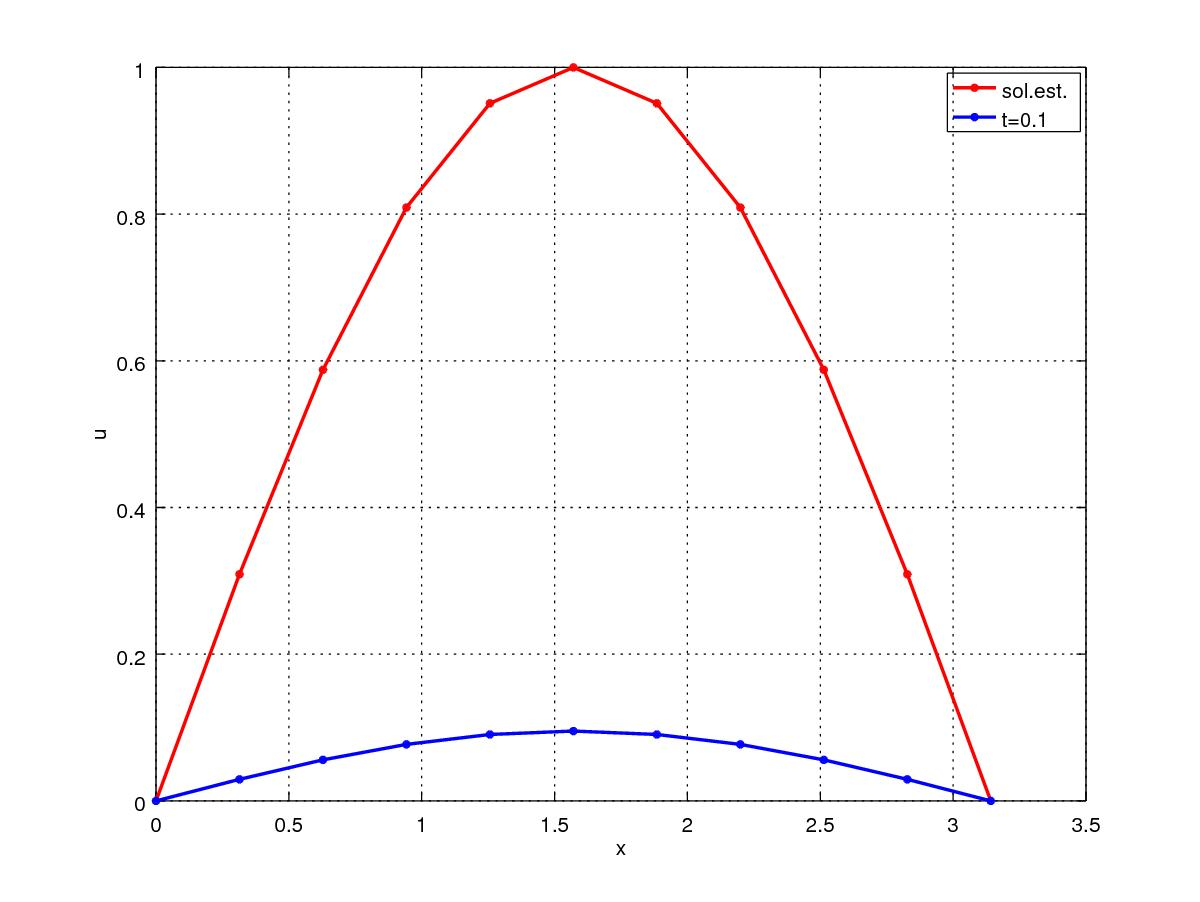
\includegraphics[width=0.45\textwidth]{./cap_edp/dados/ex_edp_calor/ex_edp_calor_t01} 
  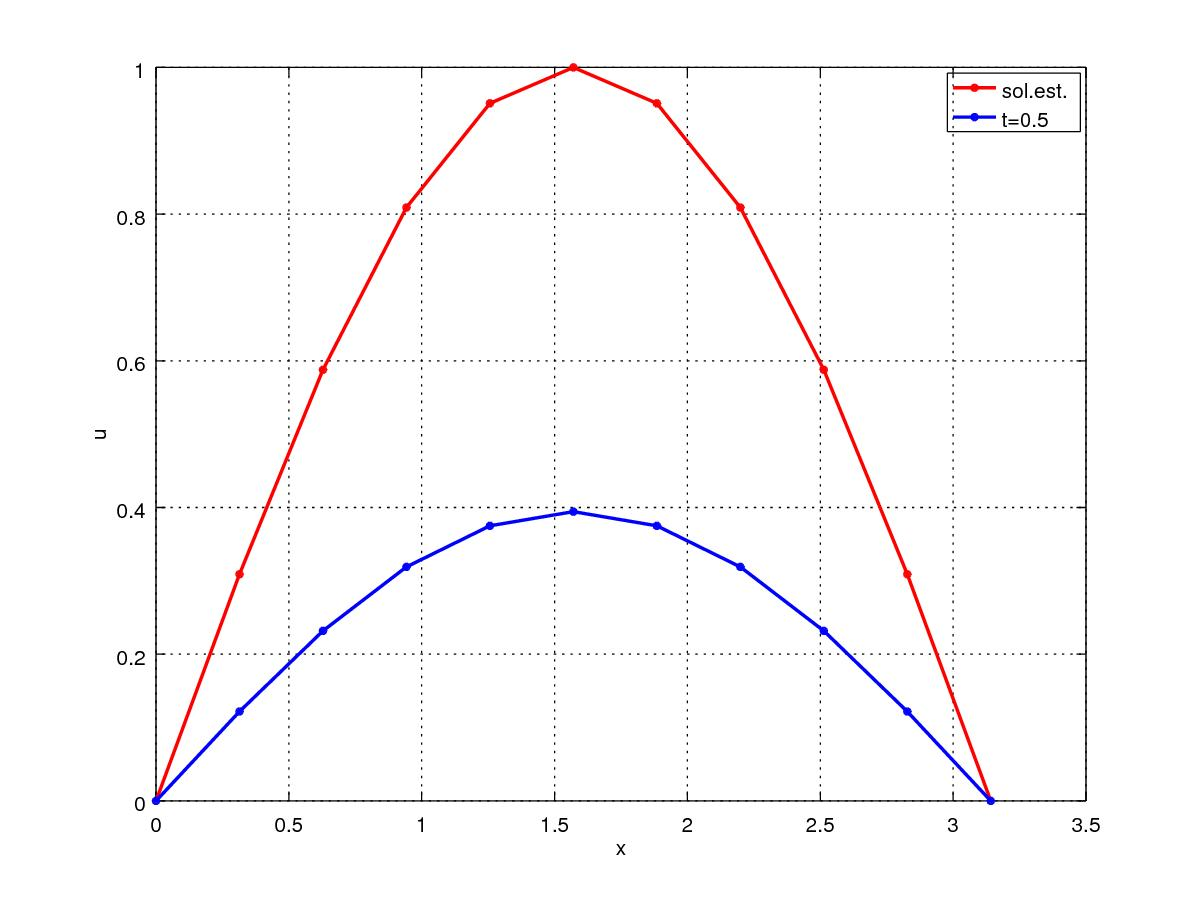
\includegraphics[width=0.45\textwidth]{./cap_edp/dados/ex_edp_calor/ex_edp_calor_t05}\\
  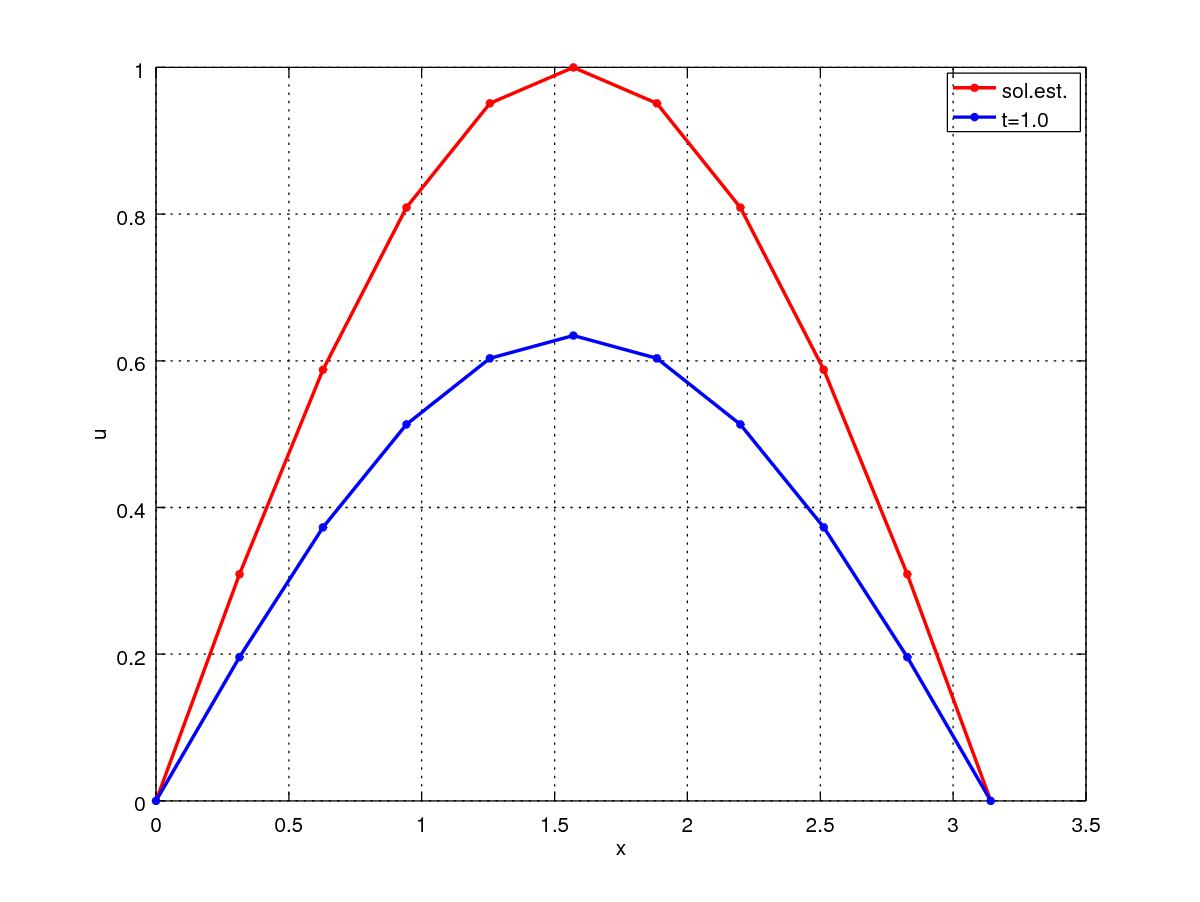
\includegraphics[width=0.45\textwidth]{./cap_edp/dados/ex_edp_calor/ex_edp_calor_t1} 
  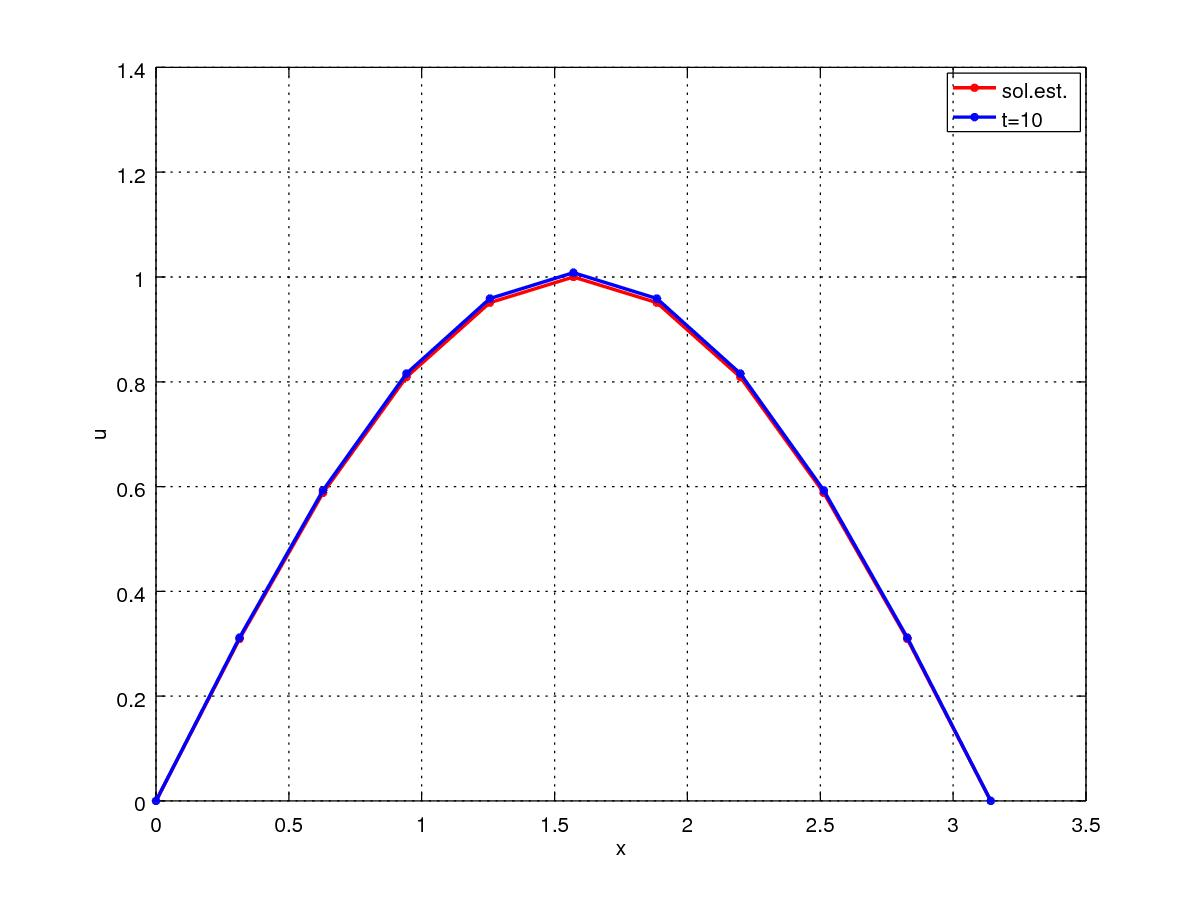
\includegraphics[width=0.45\textwidth]{./cap_edp/dados/ex_edp_calor/ex_edp_calor_t10}
  \caption{Resultados referentes ao Exemplo~\ref{ex:edp_calor}.}
  \label{fig:ex_edp_calor}
\end{figure}

Este problema tem solução estacionário $u(x) = \sen(x)$. Na Figura~\ref{fig:ex_edp_calor}, temos o esboço das soluções numéricas em diferentes tempos $t$ usando o esquema numérico acima com $h=10^{-1}$ e $h_t=10^{-3}$.

\ifisoctave
No \verb+GNU Octave+, podemos computar os resultados discutidos neste exemplo com o seguinte código:
\begin{verbatim}
#params
n=11;
h=pi/(n-1);

tf=1;
ht=10^-3;
nt=round(tf/ht)+1;

#fonte
f = @(x) sin(x);

#malha
t=[0:ht:(nt-1)*ht]'; 
x=[0:h:(n-1)*h]';

#matriz MDF
A = sparse(n-2,n-2);
A(1,1)=-2/h^2;
A(1,2)=1/h^2;
for i=2:n-3
  A(i,i-1)=1/h^2;
  A(i,i)=-2/h^2;
  A(i,i+1)=1/h^2;
endfor
A(n-2,n-3)=1/h^2;
A(n-2,n-2)=-2/h^2;

#c.i.
u=zeros(n,1);

#iter. de Euler
for k=1:nt-1
  u(2:n-1)=u(2:n-1)+ht*(A*u(2:n-1)+f(x(2:n-1)));
endfor

#visu
uest = @(x) sin(x);
plot(x,uest(x),'r.-',...
     x,u,'b.-');grid
xlabel('x');
ylabel('u');
legend('sol.est.','sol.num.');
\end{verbatim}
\fi
\end{ex}

\subsection*{Exercícios}

\begin{exer}
  Considere o seguinte problema
  \begin{align}
    u_t - u_{xx} &= f(x),~t>0,~0\leq x \leq 1,\\
    u(0,x) &= 0,~0<x<1,\\
    u(t,0) &= 1,~t>0\\
    u(t,1) &= 0,~t>0.
  \end{align}
com
\begin{equation}
  f(x) = \left\{
    \begin{array}{ll}
      1 &, x\leq 0,5,\\
      0 &, x>0,5
    \end{array}
\right.
\end{equation}
Use o método de diferenças finitas para obter uma aproximação de $u(1,0.5)$ com dois dígitos significativos de precisão.
\end{exer}
\begin{resp}
  \ifisoctave 
  \href{https://github.com/phkonzen/notas/blob/master/src/MatematicaNumerica/cap_edp/dados/exer_edp_calor_1/exer_edp_calor_1.m}{Código.} 
  \fi
  $5,6\E-1$
\end{resp}

\section{Equação da onda}\label{cap_edp_sec_onda}\index{equação!da onda}

A equação da onda definida em  $D := (x_{\text{ini}}, x_{\text{fin}})$ com condições iniciais dadas e condições de contorno de Dirichlet homogêneas refere-se o seguinte problema
\begin{align}
  u_{tt} - \alpha u_{xx} &= 0,~t>t_0,~x\in D, \label{eq:edp_onda_eq}\\
  u(x,t_0) &= f(x),~x\in D,\label{eq:edp_onda_ci1}\\
  \frac{\p u}{\p t}(x,t_0) &= g(x),~x\in D,\label{eq:edp_onda_ci2}\\
  u(x_{\text{ini}},t) &= 0,~t>t_0,\label{eq:edp_onda_bcxini}\\
  u(x_{\text{fin}},t) &= 0,~t>t_0\label{eq:edp_onda_bcxfin}
\end{align}
onde $u = u(x,t)$ é a incógnita.

Aqui, para aplicarmos o método de diferenças finitas, vamos escolher os tempos $t^{(j)} = t_0 + (j-1)h_t$, $j=1, 2, \dotsc, n_t$, com passo temporal $h_t>0$, e os pontos $x_i=x_{\text{ini}}+(i-1)h_x$, $i=1, 2, \dotsc, n_x$, com passo no espaço espacial $h_x = (x_{\text{fin}}-x_{\text{ini}})/(n_x-1)$.

Da escolha das discretizações temporal e espacial, podemos usar a fórmula de diferenças finitas de ordem $2$ para discretizarmos a equação \eqref{eq:edp_onda_eq}. Para tanto, denotamos $u_{i,j} \approx u(x_i,t_j)$ e de \eqref{eq:edp_onda_eq} temos
\begin{equation}
  \frac{u_{i,j-1}-2u_{i,j}+u_{i,j+1}}{h_t^2} - \alpha\frac{u_{i-1,j}-2u_{i,j}+u_{i+1,j}}{h_x^2} = 0,
\end{equation}
para $j=2, 3, \dotsc, n_t-1$ e $i=2, 3, \dotsc, n_x-1$. Rearranjando os termos, temos
\begin{equation}\label{eq:edp_onda_aux1}
  u_{i,j+1} = \alpha\frac{h_t^2}{h_x^2}u_{i-1,j} + 2\left(1-\alpha\frac{h_t^2}{h_x^2}\right)u_{i,j} + \alpha\frac{h_t^2}{h_x^2}u_{i+1,j} - u_{i,j-1},
\end{equation}
para $j=2, 3, \dotsc, n_t-1$ e $i=2, 3, \dotsc, n_x-1$.

Agora, das condições de contorno \eqref{eq:edp_onda_bcxini} e \eqref{eq:edp_onda_bcxfin}, temos $u_{1,j}=u_{n_x,j}=0$, $j=2, 3, \dotsc, n_t$. Com isso, o sistema \eqref{eq:edp_onda_aux1} torna-se
\begin{align}
  u_{2,j+1} &= 2\left(1-\alpha\frac{h_t^2}{h_x^2}\right)u_{2,j} + \alpha\frac{h_t^2}{h_x^2}u_{3,j} - u_{2,j-1},\\
  u_{i,j+1} &= \alpha\frac{h_t^2}{h_x^2}u_{i-1,j} + 2\left(1-\alpha\frac{h_t^2}{h_x^2}\right)u_{i,j} + \alpha\frac{h_t^2}{h_x^2}u_{i+1,j} - u_{i,j-1},\\
  u_{n_x-1,j+1} &= \alpha\frac{h_t^2}{h_x^2}u_{n_x-2,j} + 2\left(1-\alpha\frac{h_t^2}{h_x^2}\right)u_{n_x-1,j} - u_{i,j-1},\\
\end{align}
para $i=3, 4, \dotsc, n_x$ e $j=2, 3, \dotsc, n_t$. Este sistema de equações pode ser escrita na seguinte forma matricial
\begin{align}
  \begin{bmatrix}
    u_{2,j+1}\\
    u_{3,j+1}\\
    \vdots\\
    u_{n_x-1,j+1}
  \end{bmatrix}
  &=
  \begin{bmatrix}
    2(1-\lambda) & \lambda & 0 & \cdots & 0\\
    \lambda & 2(1-\lambda) & \lambda & \cdots & 0\\
    0  & \ddots & \ddots & \ddots & \cdots \\
    0  & 0 & \cdots & \lambda & 2(1-\lambda)
  \end{bmatrix}
  \begin{bmatrix}
    u_{2,j}\\
    u_{3,j}\\
    \vdots\\
    u_{n_x-1,j}
  \end{bmatrix}\nonumber\\
  &-
  \begin{bmatrix}
    u_{2,j-1}\\
    u_{3,j-1}\\
    \vdots\\
    u_{n_x-1,j-1}
  \end{bmatrix},\label{eq:edp_onda_iter3}
\end{align}
para $j=2, 3, \cdots, n_t-1$, onde $\lambda := \alpha h_t^2/h_x^2$.

Esta última equação~\eqref{eq:edp_onda_iter3} nos permite computar iterativamente a aproximação $u_{i,j+1}$ a partir das aproximações $u_{i,j}$ e $u_{i,j-1}$. Para inicializar as iterações, precisamos de $u_{i,1}$ e $u_{i,2}$, $i=2, 3, \dotsc, n_x$. A primeira é dada pela condição inicial \eqref{eq:edp_onda_ci1}, da qual temos
\begin{equation}\label{eq:edp_onda_iter1}
  u_{i,1} = f(x_i), ~i=2, 3, \dotsc, n_t.
\end{equation}
Agora, usando a fórmula de diferenças finitas progressiva de ordem $1$ na condições inicial \eqref{eq:edp_onda_ci2}, obtemos
\begin{equation}\label{eq:edp_onda_iter2}
  u_{i,2} = u_{i,1} + h_tg(x_i), ~i=2, 3, \dotsc, n_t.
\end{equation}

Com tudo isso, observamos que as equações \eqref{eq:edp_onda_iter1}, \eqref{eq:edp_onda_iter2} e \eqref{eq:edp_onda_iter3}, nesta ordem, nos fornece um algoritmo iterativo no tempo para computar as aproximações da solução $u$.

\begin{obs}
  Pode-se mostrar a seguinte condição de estabilidade
  \begin{equation}
    \alpha \frac{h_t^2}{h_x^2} \leq 1.
  \end{equation}
\end{obs}

\begin{ex}\label{ex:edp_onda}
  Consideremos o seguinte problema
  \begin{align}
    u_{tt} - u_{xx} &= 0,~t>0,~0< x < 1,\\
    u(0,x) &= x(1-x),~0<x<1,\\
    u_t(0,x) &= 0,~0<x<1,\\
    u(t,0) &= 0,~t>0\\
    u(t,\pi) &= 0,~t>0.
  \end{align}

\begin{figure}[h!]
  \centering
  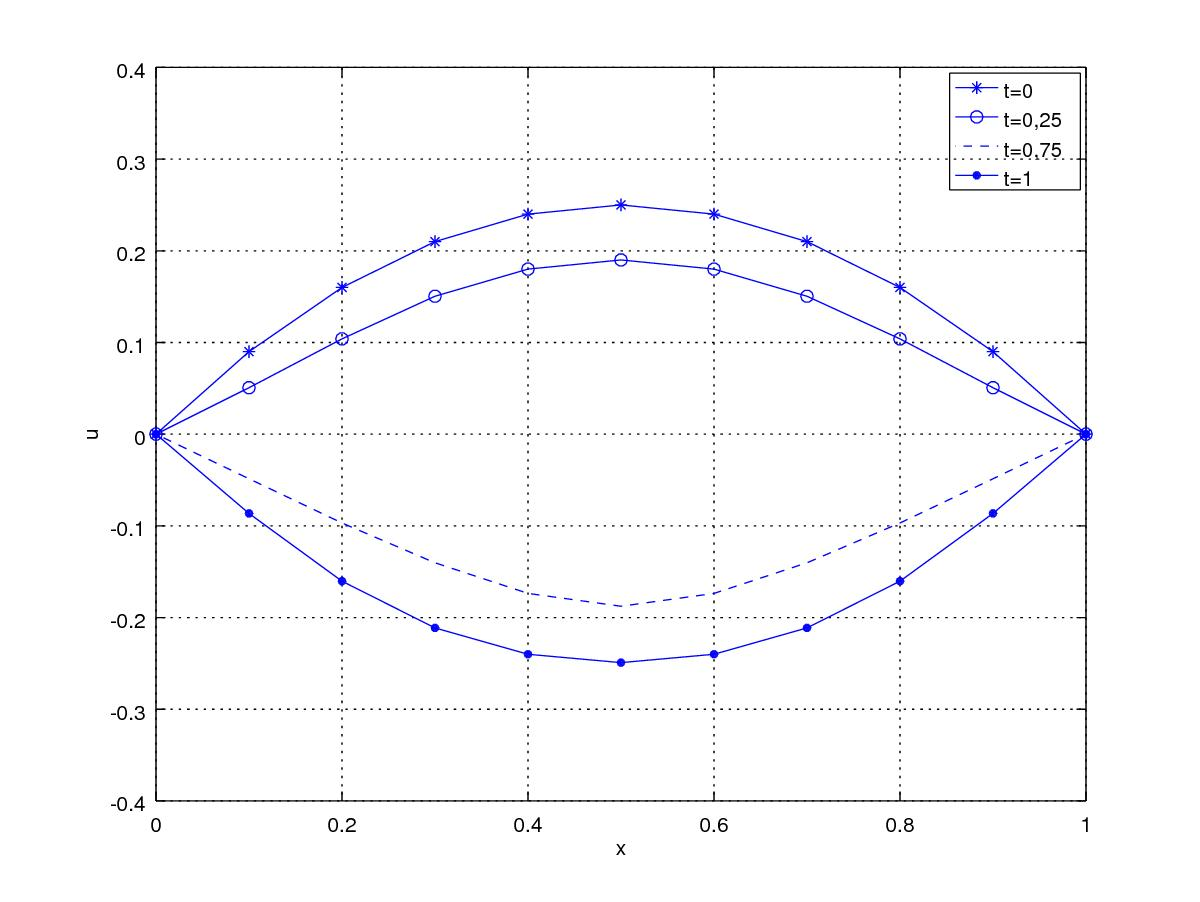
\includegraphics[width=0.8\textwidth]{./cap_edp/dados/ex_edp_onda/ex_edp_onda}
  \caption{Resultados referentes ao Exemplo~\ref{ex:edp_onda}.}
  \label{fig:ex_edp_onda}
\end{figure}

Na Figura~\ref{fig:ex_edp_onda}, temos o esboço das soluções numéricas em diferentes tempos $t$ usando o esquema numérico acima com $h_t=10^{-2}$ e $h_x=10^{-1}$.

\ifisoctave
No \verb+GNU Octave+, podemos computar os resultados discutidos neste exemplo com o seguinte código:
\begin{verbatim}
#params
nx=11;
hx=1/(nx-1);

tf=1;
ht=10^-2;
nt=round(tf/ht)+1;

lambda = ht^2/hx^2;

#malha
t=[0:ht:(nt-1)*ht]'; 
x=[0:hx:(nx-1)*hx]';

#u
u0=zeros(nx,1);
u1=zeros(nx,1);
u=zeros(nx,1);

#c.i. 1
for i=2:nx-1
  u0(i)=x(i)*(1-x(i));
endfor

#c.i. 2
u1=zeros(nx,1);
for i=2:nx-1
  u1(i)=u0(i)+ht*0;
endfor

#matriz MDF
A = sparse(nx-2,nx-2);
A(1,1)=2*(1-lambda);
A(1,2)=lambda;
for i=2:nx-3
  A(i,i-1)=lambda;
  A(i,i)=2*(1-lambda);
  A(i,i+1)=lambda;
endfor
A(nx-2,nx-3)=lambda;
A(nx-2,nx-2)=2*(1-lambda);

#iteracoes
for k=2:nt-1
  u(2:nx-1)=A*u1(2:nx-1) - u0(2:nx-1);
  u0=u1;
  u1=u;
endfor

#visu
plot(x,u1,'b-');grid
xlabel('x');
ylabel('u');
\end{verbatim}
\fi
\end{ex}

\subsection*{Exercício}

\begin{exer}
  Considere o seguinte problema
  \begin{align}
    u_{tt} - u_{xx} &= 0,~t>0,~0< x < 1,\\
    u(0,x) &= x(1-x),~0<x<1,\\
    u_t(0,x) &= 1,~0<x<1,\\
    u(t,0) &= 0,~t>0\\
    u(t,\pi) &= 0,~t>0.
  \end{align}
Use o método de diferenças finitas para obter uma aproximação de $u(0,75,~1)$ com dois dígitos significativos de precisão.
\end{exer}
\begin{resp}
  \ifisoctave 
  \href{https://github.com/phkonzen/notas/blob/master/src/MatematicaNumerica/cap_edp/dados/exer_edp_onda_1/exer_edp_onda_1.m}{Código.} 
  \fi
  $6,3\E-2$
\end{resp}

%resposta dos exercícios
\ifisbook
%Este trabalho está licenciado sob a Licença Atribuição-CompartilhaIgual 4.0 Internacional Creative Commons. Para visualizar uma cópia desta licença, visite http://creativecommons.org/licenses/by-sa/4.0/ ou mande uma carta para Creative Commons, PO Box 1866, Mountain View, CA 94042, USA.

\chapter*{Resposta dos Exercícios}\label{cap_respostas}
\addcontentsline{toc}{chapter}{Respostas dos Exercícios}

\shipoutAnswer
\fi

%references
\nocite{*}
\bibliography{main}
\addcontentsline{toc}{chapter}{Referências Bibliográficas}

\ifisbook
\clearpage
\addcontentsline{toc}{chapter}{Índice Remissivo}
\printindex
\fi

\end{document}
